\documentclass[a4paper,12pt,twoside]{ThesisStyle}

\usepackage{graphicx} 
\usepackage{array} 
\usepackage{amsmath}
\usepackage{pdfpages} 
\usepackage{natbib}
\DeclareMathOperator\erf{erf} 
\usepackage[utf8]{inputenc}
\usepackage[T1]{fontenc} 
\usepackage{ textcomp }
\usepackage{ amssymb }
\usepackage{lscape}
\usepackage{ gensymb }

\usepackage{amsmath,amssymb}             % AMS Math
% \usepackage[french]{babel}
\usepackage[latin1]{inputenc}
\usepackage[T1]{fontenc}
\usepackage[left=1.5in,right=1.3in,top=1.1in,bottom=1.1in,includefoot,includehead,headheight=13.6pt]{geometry}
\renewcommand{\baselinestretch}{1.05}

% Table of contents for each chapter

\usepackage[nottoc, notlof, notlot]{tocbibind}
\usepackage{minitoc}
\setcounter{minitocdepth}{2}
\mtcindent=15pt
% Use \minitoc where to put a table of contents

\usepackage{aecompl}

% Glossary / list of abbreviations

\usepackage[intoc]{nomencl}
\setlength{\nomitemsep}{-\parsep}
\renewcommand{\nomname}{List of notations}
\renewcommand{\nompreamble}{\markboth{List of notations}{List of notations}}
\newcommand{\nomunit}[1]{ \renewcommand{\nomentryend}{\hspace*{\fill}#1}}
\renewcommand{\nomgroup}[1]
{%
    \ifthenelse{\equal{#1}{A}}
    {\vspace{2em}\item[]\hspace*{-\leftmargin}%
    \hfill \textbf{Text abbreviations} \hfill \hbox{}}
{%
    \ifthenelse{\equal{#1}{B}}
    {\vspace{2em}\item[]\hspace*{-\leftmargin}%
    \hfill \textbf{Part I - Variables and parameters} \hfill \hbox{}}
{%
    \ifthenelse{\equal{#1}{C}}
    {\vspace{2em}\item[]\hspace*{-\leftmargin}%
    \hfill \textbf{Part II - Variables and parameters} \hfill \hbox{}}
}
}
}

\makenomenclature

% My pdf code

\usepackage{ifpdf}

\ifpdf
  \usepackage[pdftex]{graphicx}
  \DeclareGraphicsExtensions{.jpg}
  \usepackage[a4paper,pagebackref,hyperindex=true]{hyperref}
\else
  \usepackage{graphicx}
  \DeclareGraphicsExtensions{.ps,.eps}
  \usepackage[a4paper,dvipdfm,pagebackref,hyperindex=true]{hyperref}
\fi

\graphicspath{{.}{images/}}

% nicer backref links
\renewcommand*{\backref}[1]{}
\renewcommand*{\backrefalt}[4]{%
\ifcase #1 %
(Not cited.)%
\or
(Cited on page~#2.)%
\else
(Cited on pages~#2.)%
\fi}
\renewcommand*{\backrefsep}{, }
\renewcommand*{\backreftwosep}{ and~}
\renewcommand*{\backreflastsep}{ and~}

% Links in pdf
\usepackage{color}
\definecolor{linkcol}{rgb}{0,0,0.4} 
\definecolor{citecol}{rgb}{0.5,0,0} 

% Change this to change the informations included in the pdf file

% See hyperref documentation for information on those parameters

\hypersetup
{
bookmarksopen=true,
pdftitle="Design and Use of Anatomical Atlases for Radiotherapy",
pdfauthor="Olivier COMMOWICK", 
pdfsubject="Creation of atlases and atlas based segmentation", %subject of the document
%pdftoolbar=false, % toolbar hidden
pdfmenubar=true, %menubar shown
pdfhighlight=/O, %effect of clicking on a link
colorlinks=true, %couleurs sur les liens hypertextes
pdfpagemode=None, %aucun mode de page
pdfpagelayout=SinglePage, %ouverture en simple page
pdffitwindow=true, %pages ouvertes entierement dans toute la fenetre
linkcolor=linkcol, %couleur des liens hypertextes internes
citecolor=citecol, %couleur des liens pour les citations
urlcolor=linkcol %couleur des liens pour les url
}

% definitions.
% -------------------

\setcounter{secnumdepth}{3}
\setcounter{tocdepth}{2}

% Some useful commands and shortcut for maths:  partial derivative and stuff

\newcommand{\pd}[2]{\frac{\partial #1}{\partial #2}}
\def\abs{\operatorname{abs}}
\def\argmax{\operatornamewithlimits{arg\,max}}
\def\argmin{\operatornamewithlimits{arg\,min}}
\def\diag{\operatorname{Diag}}
\newcommand{\eqRef}[1]{(\ref{#1})}

\usepackage{rotating}                    % Sideways of figures & tables
%\usepackage{bibunits}
%\usepackage[sectionbib]{chapterbib}          % Cross-reference package (Natural BiB)
%\usepackage{natbib}                  % Put References at the end of each chapter
                                         % Do not put 'sectionbib' option here.
                                         % Sectionbib option in 'natbib' will do.
\usepackage{fancyhdr}                    % Fancy Header and Footer

% \usepackage{txfonts}                     % Public Times New Roman text & math font
  
%%% Fancy Header %%%%%%%%%%%%%%%%%%%%%%%%%%%%%%%%%%%%%%%%%%%%%%%%%%%%%%%%%%%%%%%%%%
% Fancy Header Style Options

\pagestyle{fancy}                       % Sets fancy header and footer
\fancyfoot{}                            % Delete current footer settings

%\renewcommand{\chaptermark}[1]{         % Lower Case Chapter marker style
%  \markboth{\chaptername\ \thechapter.\ #1}}{}} %

%\renewcommand{\sectionmark}[1]{         % Lower case Section marker style
%  \markright{\thesection.\ #1}}         %

\fancyhead[LE,RO]{\bfseries\thepage}    % Page number (boldface) in left on even
% pages and right on odd pages
\fancyhead[RE]{\bfseries\nouppercase{\leftmark}}      % Chapter in the right on even pages
\fancyhead[LO]{\bfseries\nouppercase{\rightmark}}     % Section in the left on odd pages

\let\headruleORIG\headrule
\renewcommand{\headrule}{\color{black} \headruleORIG}
\renewcommand{\headrulewidth}{1.0pt}
\usepackage{colortbl}
\arrayrulecolor{black}

\fancypagestyle{plain}{
  \fancyhead{}
  \fancyfoot{}
  \renewcommand{\headrulewidth}{0pt}
}

\usepackage{algorithm}
\usepackage[noend]{algorithmic}

%%% Clear Header %%%%%%%%%%%%%%%%%%%%%%%%%%%%%%%%%%%%%%%%%%%%%%%%%%%%%%%%%%%%%%%%%%
% Clear Header Style on the Last Empty Odd pages
\makeatletter

\def\cleardoublepage{\clearpage\if@twoside \ifodd\c@page\else%
  \hbox{}%
  \thispagestyle{empty}%              % Empty header styles
  \newpage%
  \if@twocolumn\hbox{}\newpage\fi\fi\fi}

\makeatother
 
%%%%%%%%%%%%%%%%%%%%%%%%%%%%%%%%%%%%%%%%%%%%%%%%%%%%%%%%%%%%%%%%%%%%%%%%%%%%%%% 
% Prints your review date and 'Draft Version' (From Josullvn, CS, CMU)
\newcommand{\reviewtimetoday}[2]{\special{!userdict begin
    /bop-hook{gsave 20 710 translate 45 rotate 0.8 setgray
      /Times-Roman findfont 12 scalefont setfont 0 0   moveto (#1) show
      0 -12 moveto (#2) show grestore}def end}}
% You can turn on or off this option.
% \reviewtimetoday{\today}{Draft Version}
%%%%%%%%%%%%%%%%%%%%%%%%%%%%%%%%%%%%%%%%%%%%%%%%%%%%%%%%%%%%%%%%%%%%%%%%%%%%%%% 

\newenvironment{maxime}[1]
{
\vspace*{0cm}
\hfill
\begin{minipage}{0.5\textwidth}%
%\rule[0.5ex]{\textwidth}{0.1mm}\\%
\hrulefill $\:$ {\bf #1}\\
%\vspace*{-0.25cm}
\it 
}%
{%

\hrulefill
\vspace*{0.5cm}%
\end{minipage}
}

\let\minitocORIG\minitoc
\renewcommand{\minitoc}{\minitocORIG \vspace{1.5em}}

\usepackage{multirow}
%\usepackage{slashbox}

\newenvironment{bulletList}%
{ \begin{list}%
	{$\bullet$}%
	{\setlength{\labelwidth}{25pt}%
	 \setlength{\leftmargin}{30pt}%
	 \setlength{\itemsep}{\parsep}}}%
{ \end{list} }

\newtheorem{definition}{D�finition}
\renewcommand{\epsilon}{\varepsilon}

% centered page environment

\newenvironment{vcenterpage}
{\newpage\vspace*{\fill}\thispagestyle{empty}\renewcommand{\headrulewidth}{0pt}}
{\vspace*{\fill}}



\usepackage{makeidx} 
\makeindex

\begin{document}

\begin{titlepage}
\begin{center}
\noindent {\large \textbf{Institut de Physique du Globe de Paris}} \\
\vspace*{0.3cm}
\noindent {\LARGE \textbf{Ecole doctorale des Sciences de la Terre}} \\
\vspace*{0.5cm}
\noindent \Huge \textbf{Thèse de Doctorat} \\
\vspace*{0.3cm}
\noindent \large {pour l'obtention du titre de} \\
\vspace*{0.3cm}
\noindent \LARGE \textbf{Docteur en Science} \\
\vspace*{0.3cm}
\noindent \Large de l'Institut de Physique du Globe de Paris \\
\noindent \Large \textbf{Specialité : \textsc{Geophysique}}\\
\vspace*{0.4cm}
\noindent \large {Soutenue par\\}
\noindent \LARGE Cl\'ement \textsc{Thorey} \\
\vspace*{0.8cm}
\noindent {\Huge \textbf{Magmatisme intrusif sur les planètes telluriques}} \\
\vspace*{0.8cm}
\noindent \Large \'Equipe \textsc{Plan\'etologie et Sciences Spatiales},\\
\vspace*{0.2cm}
\noindent \large Défendue le 5 Décembre, 2013. \\
\vspace*{0.5cm}
\end{center}
\noindent \large \textbf{Jury :} \\
\begin{center}
\noindent \large 
\begin{tabular}{llcl}
  \textit{Directeur:} & Chlo\'e \textsc{Michaut} & - & IPGP (Paris) \\
  \textit{Co-directeur:}  & Mark  \textsc{Wieczorek}  &  - &  IPGP (Paris) \\
  \textit{Rapporteur :} &Jerome \textsc{Neufeld} & -& DAMPT (Cambridge)\\
  \textit{Rapporteur :} & Virginie \textsc{Pinel} & - & IRD (Chambéry)\\
  \textit{Examinateur :} & Oded \textsc{Aharonson} & - & WIS (Rehovot)\\
  \textit{Examinateur :} & Edouard \textsc{Kaminksi}& - & IPGP (Paris)
\end{tabular} 

% \vfill
% \includegraphics[height=2.5cm]{images/logos/ED.png}
% \hspace{0.4cm}
% \includegraphics[height=2.5cm]{images/logos/ipgp.png}
% \hspace{0.4cm}
% \includegraphics[height=2.5cm]{images/logos/IDF.png}
% \hspace{0.4cm}
% \includegraphics[height=2.5cm]{images/logos/DLR.jpeg}
% \hspace{0.4cm}
% \includegraphics[height=2.5cm]{images/logos/pres.png}

\end{center}
\end{titlepage}
\sloppy


\titlepage

%%% Local Variables:
%%% mode: latex
%%% TeX-master: "main"
%%% End:


\dominitoc
\setcounter{tocdepth}{2}

\cleardoublepage

\thispagestyle{plain}
\begin{flushleft}
 \Large
 \vspace{.5cm}
 \textbf{Remerciements}
\end{flushleft}

Cette thèse prend sûrement racine quelques années avant son début, sur
les flancs chauds et humides du volcan ``El Fuego'' au Mexique. En
effet, c’est sans doute ce volcan qui a piqué en premier ma curiosité
pour les sciences de la Terre. Je commencerais donc par remercier Nick
Varley : sa passion sans limites ainsi qu’une légère touche
d’insouciance nous auront toutes deux permis d’effleurer au plus près
la beauté et la puissance de ce volcan capricieux. À Colima, je ne
puis aussi oublier Jannes, Irving, Pilar, Ana et toutes les personnes
que j’ai pu croiser sur mon chemin. À tous, merci pour cette
expérience inoubliable.

Durant cette période, je remercie aussi mes parents d’avoir supporté
ces longs mois sans nouvelles. Merci à vous pour le soutien
inconditionnel que vous m’avez apporté durant toutes mes années
d’études. Même si le fond vous restera sans doute un peu nébuleux,
sachez que cette thèse vous doit beaucoup.

Ces travaux n’auraient pas non plus vu le jour sans Chloé Michaut, ma
directrice de thèse. Je ne peux que la remercier pour sa patience et
son accompagnement tout au long de ces trois ans, pour tout ce qu’elle
m’a apporté scientifiquement et personnellement. Une liste de
remerciements non exhaustive contiendrait sûrement la faculté de suivre
l’évolution de ma pensée souvent embrumée, de décrypter mes notes
interminables, d’apprécier mes figures colorées, de relire mes
manuscrits pas finis et surtout, de m’avoir toujours encouragé et de
m’avoir laissé explorer à mon rythme sans me laisser pour autant
m’égarer.

Ce travail,  et notamment la  digression champ de gravité,  doit aussi
beaucoup  à  Mark Wieczorek.  Merci  de  m’avoir laissé  triturer  les
dernières données de  la mission GRAIL, de m’avoir guidé  tout au long
de cette  étude ainsi que de  m’avoir permis de présenter  mes travaux
dans le Colorado. Je remercie les  membres de mon jury d’avoir accepté
d’évaluer  ce  travail,  car  j’imagine  qu’il  existe  lectures  plus
agréables  pour la  rentrée  : Jerome  Neufeld,  Virginie Pinel,  Oded
Aharonson et Edouard Kaminksi.

Sous les auspices  de Lamarck, je remercie aussi  toutes les personnes
qui ont contribué de  près ou de loin au bon  déroulement de ces trois
années.   Tout  d’abord  Mathieu  pour ses  conseils,  les  bavardages
lunaires  et  les sessions  d’escalade  qui  ont accompagné  toute  ma
première année, Sebastiano  et Karine pour leur énergie  et leur bonne
humeur qui se  chargèrent de la deuxième et enfin,  Alicia, Shang Xia,
Claudine, Mélanie, Jean-François, Lucile, Sébastien, Yasuhiro, Foivos,
Virgile,   Joana  et   toutes  les   personnes  du   laboratoire  de
planétologie  et sciences  spatiales de  l’IPGP et  d'AIM que  j’ai pu
oublier devant  l’explosion démographique qui  a eu lieu  durant cette
dernière année.

Sous la  bienveillance de  Jussieu, je remercie  tout particulièrement
Adrien et Kenny, avec qui j’ai  passé beaucoup de temps à procrastiner
au Linnée.   Je remercie aussi  l'intégralité de  la TP team  avec qui
j'ai pris plaisir  à enseigner la physique.  Je ne  peux enfin oublier
Malbec,  le cluster  qui, heure  après heure,  jour après  jour, s’est
affairé aux  tâches que je  lui avais  donné sans rechigner.   Merci à
Alexandre de nous avoir présenté  et au service informatique de l’IPGP
qui le bichonne et l’entretient depuis sa création.

Enfin,   dans  cette   épopée  parisienne,   je  remercie   aussi  mes
indénombrables colocs de la rue  Tolbiac, avec une pensée particulière
pour M.   Nicolas, et les  gens du swing  et de l’escalade.   Un merci
tout particulier  à Valentin et CamCam  qui ont aussi participé  à mon
équilibre  parisien. Merci  aussi  à  mon voisin  du  dessus, rue  des
Gobelins, de m’avoir réveillé  ``délicatement'' tous les matins, c’est
peut-être grâce à  lui que j’ai pu  finir ce travail à  temps. Dans le
camp des  anonymes, je remercie l’homme  au marcel bleu avec  qui j’ai
partagé mes  séances de courses à  pied. Bien qu’elles ne  m’aient pas
apporté d’idées révolutionnaires, ces séances m’auront au moins permis
de me vider la tête.

Je remercie également Clémentine,  Fabian (Pura Vida), Amélie, Adrien,
Lucie, Simon, Mylène et compagnie qui m’accompagnent depuis nos écoles
lyonnaises, avec une  pensée toute particulière pour  Florian, qui m’a
guidé jusque là-bas.

Enfin, je remercie Marion, pour tout !











\vspace{2cm}

%%% Local Variables:
%%% mode: latex
%%% TeX-master: "main"
%%% End:


\cleardoublepage


\thispagestyle{fancy}
\begin{center}
    \Large
    \textbf{Abstract}
\end{center}

\textbf{Key words}: Magmatic intrusions, Elastic-plated gravity
current, Thermal processes, Rheology, Temperature-dependent viscosity,
Elastic  sheet,   Laccolith,  Sill,  Earth,  Moon,   Low-slope  domes,
Floor-fractured craters, Elastic-sheet thickness, Crater depression,
Gravitational anomalies.\\

Intrusive  magmatism  plays a  fundamental  role  in the  accretionary
processes of terrestrial  crust.  Indeed, when magma is  forced to the
surface, only a small amount of  it actually reaches that level.  Most
of the  magma is intruded  into the crust  where it solidifies  into a
wide range of  features, from the small scale sills  and laccoliths to
large  scale  batholiths (several  hundred  kilometers  in size).  The
topographic deformation that could be caused by shallow intrusions can
be constrained by observations of planetary surfaces; that is, volume,
shape and other dimensions of  intrusions can be quantified.  However,
such  observations  must be  linked  to  dynamic  models of  of  magma
emplacement at depth in order  to provide insights into magma physical
properties,  injection  rate,  emplacement  depth  and  the  intrusion
process itself.

In  this  thesis,  we  first  investigate  the  relation  between  the
morphology  of shallow  intermediate-scale magmatic  intrusions (sills
and  laccoliths)  and their  cooling.   We  propose  a model  for  the
spreading   of    an   elastic-plated    gravity   current    with   a
temperature-dependent viscosity  that accounts  for a  realistic magma
rheology, melt crystallization and  heating of the surrounding medium.
The  mechanisms that  drive cooling  of the  intrusions vary  from the
Earth to the Moon and the ability  of the model to reproduce the final
morphologies (aspect  ratio) of  terrestrial laccoliths  and low-slope
lunar domes is examined.

On the  Moon, emplacement  of magmatic intrusions  into the  crust has
also  been proposed  as  a  possible mechanism  for  the formation  of
floor-fractured  craters.  We  propose a  model for  an elastic-plated
gravity current  spreading beneath  an elastic overburden  of variable
thickness.  We  find that  several characteristics  of floor-fractured
craters are indeed  consistent with the emplacement of  a large volume
of magma  beneath their floor.   In addition, using  the unprecedented
resolution  of the  NASA's  Gravity Recovery  and Interior  Laboratory
(GRAIL) mission,  in combination  with topographic data  obtained from
the  Lunar Orbiter  Laser Altimeter  (LOLA) instrument,  we show  that
lunar   floor-fractured   craters  present   gravitational   anomalies
consistent with magmatic intrusions intruding a crust characterized by
a $12\%$  porosity. The implications  in terms of lunar  evolution are
examined.

%%% Local Variables:
%%% mode: latex
%%% TeX-master: "main"
%%% End:

\thispagestyle{fancy}
\begin{center}
 \Large
 \textbf{Résumé}
\end{center}

\textbf{Mots-clés} : Intrusion magmatique, Écoulement gravitaire sous
une plaque élastique, Refroidissement, Rhéologie, Viscosité dépendante
de la température, Fléchissement d'une plaque élastique, Laccolite,
Sill, Terre, Lune, Dômes à faible pente, Cratères d' impacte, Cratère
au sol fracturé, Anomalie gravitaire.\\

Le magmatisme intrusif est une source masquée, mais potentiellement
importante du magmatisme planétaire. En effet, les magmas, formaient au
sein du manteau, n'atteignent que rarement la surface. La grande
majorité se met en place et refroidit au sein de la croûte sous forme
d'intrusions magmatiques. Le volume ainsi que la morphologie de ces
intrusions peuvent être contraints par l’observation des surfaces
planétaires. Cependant, en l'absence d'un modèle capable de décrire la
mise en place de telles intrusions, il est difficile de se faire une
idée des propriétés physiques de l'écoulement et des magmas eux même.

Dans cette thèse, nous commençons par nous intéresser à la relation
qui existe entre la morphologie finale des intrusions de tailles
intermédiaires (sills et laccolites) et l'écoulement lui-même. Nous
proposons ainsi un modèle dynamique de la mise en place de l’intrusion
qui prend en compte une rhéologie réaliste pour le magma, l'énergie
libérée par sa cristallisation ainsi que le chauffage de l'encaissant.
Les conditions varient de la Terre à la Lune; nous examinons ainsi la
capacité du modèle à reproduire la morphologie de ces intrusions dans
ces deux différents contextes planétaires.

Sur la Lune,  la mise en place d'intrusions magmatiques  au sein de la
croûte a  aussi été proposée  pour expliquer les  déformations subites
par  certains  cratères  après  leurs formations.  Pour  tester  cette
hypothèse, nous proposons un modèle d'étalement d'intrusion magmatique
sous une dépression caractéristique de l'impact. Nous montrons que les
différentes déformations observées  au sein de ces  cratères sont bien
en accord  avec la mise  en place  d'importants volumes de  magma sous
leur sol. De plus, en utilisant la résolution sans précédente du champ
de gravité lunaire obtenue par la  mission GRAIL, nous montrons que la
plupart  de  ces cratères  montrent  bien  des anomalies  de  gravité;
anomalies impliquant notamment une  importante porosité dans la croûte
lunaire. Les implications en terme d'évolution lunaire sont finalement
évoquées.

%%% Local Variables:
%%% mode: latex
%%% TeX-master: "main"
%%% End:


\tableofcontents

\mainmatter
\part{Dynamique des magmas à faible profondeur}

\pagestyle{fancy}

\chapter{Magmatisme intrusif}
\label{chap1}
\minitoc

\section{Formation, transport et stockage des magmas}
\label{sec:magm-intr-un}

\subsection{Formation}
\label{sec:formation-1}


La majorité des magmas sont formées par fusion partielle des roches du
manteau  supérieurs.   Cependant,  dans  les  conditions  normales  de
pression,  la température  du manteau  supérieur n'est  pas suffisante
pour  provoquer la  fusion partielle  des roches  mantelliques (Figure
\ref{Geoterme}) et  d'autres mécanismes  sont nécessaires  pour amener
les roches  du manteau à croiser  leur liquidus.  Au niveau  des zones
d'extension, i.e. au niveau des  dorsales océaniques par exemple ou au
sein des  panaches mantelliques, la  fusion partielle est  ainsi causé
par décompression  des roches  mantelliques.  Au  niveau des  zones de
subduction, les mécanismes  mises en jeux sont plus  complexes et font
intervenir la  déshydratation par  chauffage des roches,  la migration
des fluides provoquant la fusion des roches alentours.

\begin{figure}
  \begin{center}
    \graphicspath{ {/Users/thorey/Documents/These/Manuscript/Figure/Chapter1/} }
    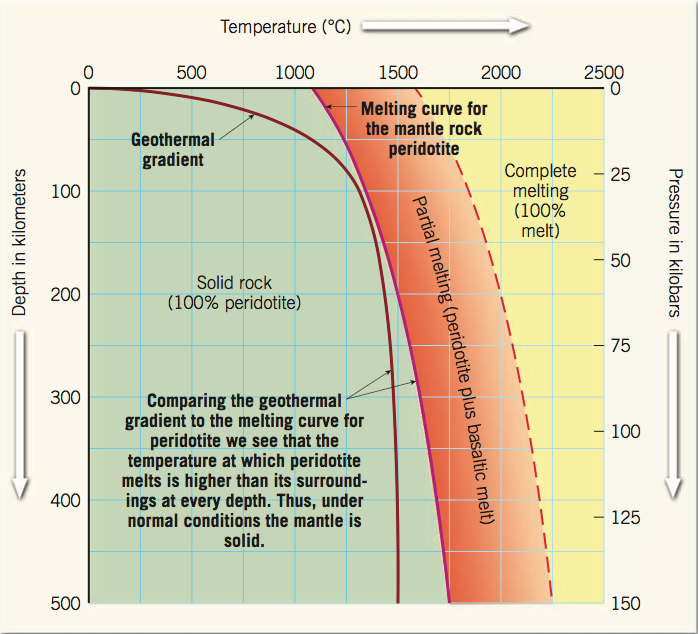
\includegraphics[scale=0.4]{geoterme.png}
    \caption{Temperature ($\°C$)  versus depth (km).   Reproduced from
      \citet{Tarbuck:1998ud}.}
    \label{Geoterme}
  \end{center}
\end{figure}

\subsection{Transport}
\label{sec:transport}

Les liquides de  fusions ainsi formés sont moins dense  que les roches
solides alentours et s'élèvent donc,  par compaction et percolation au
travers          de           la          matrice          mantellique
\citep{McKenzy:1984bo,McKenzie:1985jq}. Le magma,  liquide de fusion +
cristaux, s'accumule ensuite au sein de  chenaux, i.e.  de dykes ou le
long  de  faille  pré-existantes  pour remonter  rapidement  vers  les
couches          superficielles          de         la          croûte
\citep{Lister:1991ut,Clemens:1992kr,Petford:1993bk,Rubin:1995upa}.  En
effet, bien  que l'idée du magma  remontant lentement au sein  de gros
volume  diapirique est  encore  parfois  invoqué au  sein  de la  base
ductile  de  la   croûte  \citep{Weinberg:1994jg,Weinberg:1996vb},  le
transport rapide  du magma  au sein  des dykes  permet de  résoudre de
nombreux problèmes,  thermiques et  mécaniques, associés à  la remonté
diapirique  de gros  volume de  magma au  sein des  parties supérieurs
fragiles de la croûte invoquée historiquement \citep{Miller:1999km}.

\subsection{Stockage}
\label{sec:stockage}

Historiquement, les  travaux de  \citet{Walker:1989jq} ont  montré que
les  magmas  remontent jusqu'à  rencontrer  leur  zone de  flotabilité
neutre, une région ou la densité de la roche encaissante est proche de
celle du magma lui même. En effet, au dessus de cette couche, le magma
est plus dense  que la roche encaissante et  sa flotabilité l'entraîne
vers    le    bas.     De   nombreux    travaux,    tant    théoriques
\citep{Lister:1991ut,Petford:1993bk,Rubin:1995upa}  que  expérimentaux
\citep{Taisne:2009kj,Taisne:2011do}  ont en  effet  depuis montré  que
l'ascension  d'un dyke  était contrôlé  par la  différence de  densité
entre la  tête de celui  ci et la  roche encaissante. Lorsque  le dyke
entre dans  une région de  densité inférieure, la  surpression induite
peut, sous  certaines conditions, conduire  à l'étalement du  magma au
niveau   de   la  base   de   la   région   de  plus   forte   densité
\citep{Taisne:2011do}. Le magma s'étale donc  par gravité à la base de
cette  couche permettant  ainsi la  formation de  réservoir magmatique
sous forme d'intrusion magmatique au sein de la croûte. L’existence et
la  localisation de  cette zone  de  flottabilité neutre,  et donc  la
question de l'éruptabilité  d'un magma, dépend de  la densité relative
entre la  croûte et le  magma.  Elle dépend  donc non seulement  de la
nature  de la  croûte,  i.e.   de sa  composition,  mais  aussi de  sa
porosité,  de la  composition du  magma, de  sa température  et de  sa
teneur en volatils, qui varie, elle,  largement avec la pression et la
profondeur.

Plus  récemment, d'autres  études  ont montré  que  les contrastes  de
rigidité  entre les  différentes  couches  crustales pourraient  aussi
jouer un  rôle non  négligeable sur l'arrêt  de l'ascension  des dykes
\citep{Menand:2011ki}.   En  effet,   des  expériences  réalisées  par
\citet{Kavanagh:2006ig} ont  montré que la propagation  d'un dyke peut
être  arrêté quand  celui ci  rencontre  une interface  qui sépare  un
milieu  plus  rigide  surplombant   un  milieu  moins  rigide  (Figure
\ref{Neutral_Zone}). Le  dyke arrête ainsi son  ascension verticale et
s'étale horizontalement juste en dessous de la couche de rigidité plus
élevée. Ce  mécanisme est d'autant  plus efficace que le  contraste de
rigidité est important \citep{Kavanagh:2006ig}.

\begin{figure}
  \begin{center}
    \graphicspath{ {/Users/thorey/Documents/These/Manuscript/Figure/Chapter1/} }
    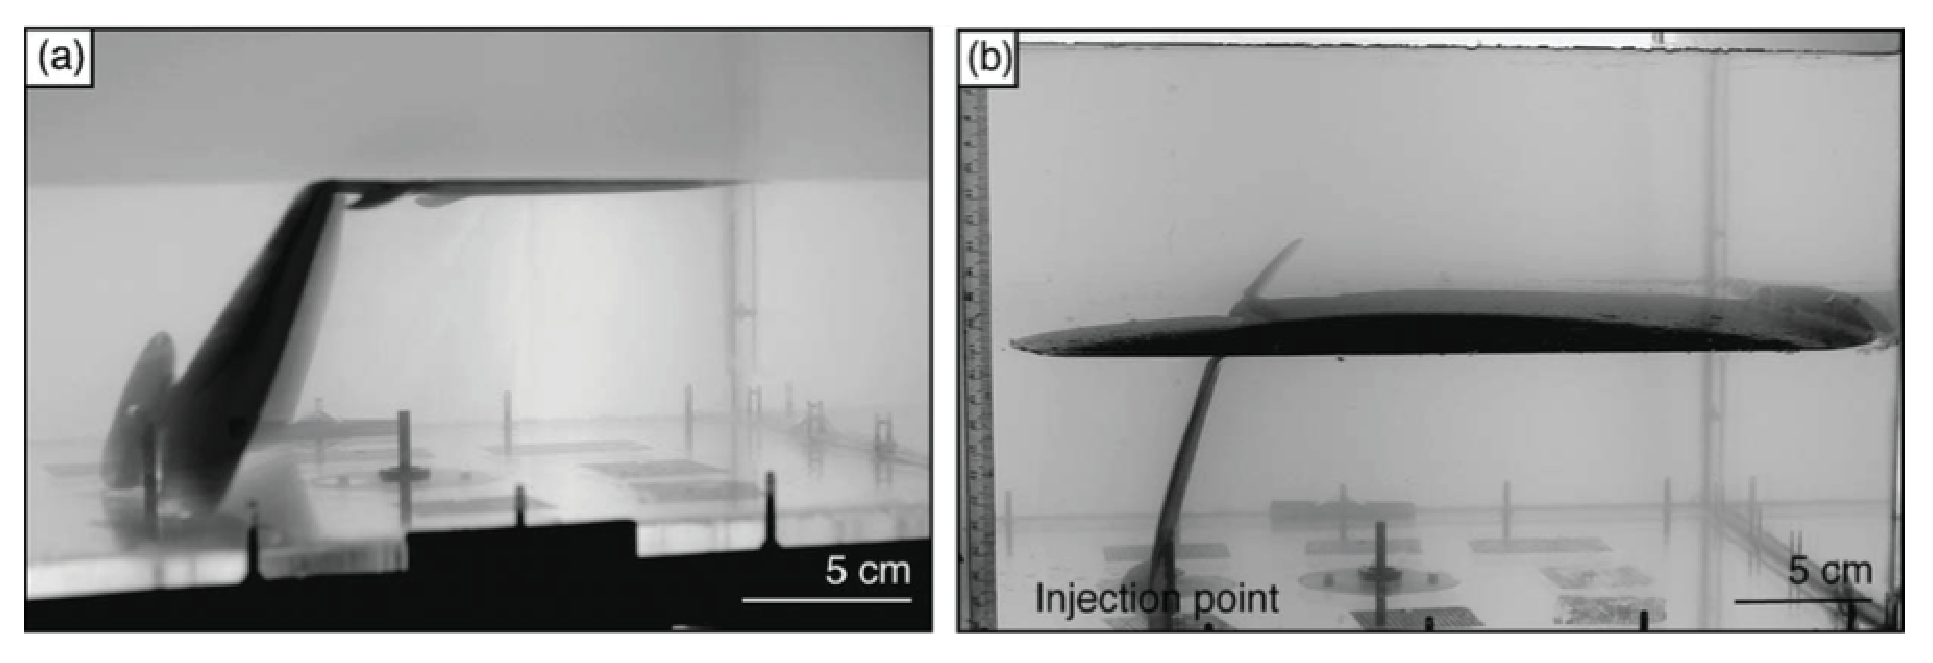
\includegraphics[scale=0.4]{Neutral_Zone.eps}
    \caption{a)  Photographie de  deux des  expériences réalisées  par
      \citet{Kavanagh:2006ig}   sur  le   comportement  d'un   dyke  à
      l'interface entre  deux milieux de rigidités  différentes. a) Le
      contraste de rigidité est très important et le dyke s'étale sous
      la couche de  rigidité importante.  b) Le  contraste de rigidité
      est plus faible et, tout en s'étalant en dessous de la couche de
      rigidité  supérieur, le  dyke  continue sa  progression dans  le
      milieu plus rigide.}
    \label{Neutral_Zone}
  \end{center}
\end{figure}


Finalement, les contraintes, locales ou globales, peuvent aussi dévier
la trajectoire d'un dyke et influencer  les trajets des magmas au sein
de la  croûte.  En  effet, des  études ont  montré que  les intrusions
magmatiques tendent  à se propager perpendiculairement  à la direction
des contraintes de  compressions \citep{Anderson:L5JA3dNN}.  Les dykes
ont donc tendance à exister dans  des situations ou les contraintes de
compressions sont horizontales  et donc à s'arrêter quand  le champ de
contrainte  évolue,  d'une  contrainte  de  compression  horizontal  à
vertical  comme  c'est le  cas  par  exemple  au niveau  des  édifices
volcaniques \citep{Pinel:2000wa,Pinel:2004ji,Roman:2014hw}.

Cependant, si  ces différents  facteurs jouent  sûrement tous  un rôle
dans  le transport  et le  stockage des  magmas au  sein de  la croûte
terrestre, la densité relative du magma et de la roche encaissante est
certainement le facteur déterminant dans  la mise en place d'intrusion
magmatiques et  la structure en  densité d'une croûte  planétaire joue
donc un rôle essentielle dans le stockage des magmas.

\section{Caractérisation du  magmatisme intrusif à  faible profondeur:
  apport des observations}
\label{sec:zool-des-intr}

\subsection{Intrusion magmatique sur Terre}
\label{sec:definition}

La croûte terrestre continentale, épaisse en moyenne de $35$ km, a une
densité  moyenne proche  de $2900$  kg m$^{-3}$.   De part  sa densité
relativement basse, elle constitue un filtre efficace à la remonté des
magmas en surface qui  sont par conséquence préférentiellement stockés
en profondeur.  \citet{Crisp:1984dm}  et \citet{White:2006gr} estiment
en effet à  $10$ fois supérieur au volume de  lave extrudé les volumes
de magma intrudés  au sein de la croûte  continentale.  Les mouvements
tectoniques  au sein  de  la  croûte ainsi  que  l’érosion ont  exposé
nombreuses  de ces  intrusions magmatiques  à la  surface. La  mise en
place  ces  magmas  en  profondeurs et  leur  solidification  semblent
résulter en une grande variété  de morphologie et de type d'intrusions
différentes dépendante des conditions, profondeurs et caractéristiques
mécaniques du milieu encaissant au moment de la formation.

Les batholiths  sont de  loin les plus  imposants représentant  de ces
familles  d'intrusions  magmatiques.   Ils peuvent  atteindre  jusqu'à
quelques  kilomètres d'épaisseur  et  s'étendre sur  des centaines  de
kilomètres.   Par  exemple, le  batholith  de  Sierra Nevada  est  une
intrusion granitique qui s'étend sur  presque la totalité de la Sierra
Nevada en Californie.  Il est maintenant clair que la mise en place de
ces gigantesques volumes de magmas  se forme par incréments successifs
de petits  volume de magma se  solidifiant lors de leur  mise en place
sur   de  longues   échelle   de  temps   $10^5$   to  $10^6$   années
\citep{Petford:2000cc,Glazner:2004gv}. Dans cette thèse, on va donc se
focaliser sur  les mécanismes de  formations et  de mise en  places de
plus  petit volume  de  magma  dans la  partie  fragile  de la  croûte
continental, des profondeurs inférieurs à $10$ km.

On  distingue généralement  deux types  d'intrusions magmatiques:  les
intrusions discordantes, qui se mettent en place perpendiculairement à
la   stratification  naturelle   de  la   croûte  et   les  intrusions
concordantes,  qui  se  mettent  en  place  parallèlement  aux  couche
géologiques. Des études géologiques de  terrain ont montré la présence
de   quatre  grandes   familles  d'intrusions   magmatique  à   faible
profondeur.

\begin{figure}
  \begin{center}
    \graphicspath{ {/Users/thorey/Documents/These/Manuscript/Figure/Chapter1/} }
    \includegraphics[scale=0.5]{Intrusive_Activity.eps}
    \caption{a) Différentes formes  du magmatisme intrusif: batholith,
      dyke,  sill   et  laccolith.    Dimensions  typiques   pour  des
      laccoliths,   dyke  et   sill  de   composition  et   d'origines
      différentes repris de \citet{Cruden:tg}. }
    \label{Dimension}
  \end{center}
\end{figure}

\begin{itemize}
\item  Les  dykes,  par  lesquels  remontent le  magma  à  travers  la
  lithosphère sont discordants et  caractérisé par de faibles rapports
  d'aspects (Figure \ref{Dimension}, \ref{picture} a).  Leur épaisseur
  peut  varier  de quelques  mètres  à  quelques centaines  de  mètres
  d'épaisseur      \citep{Walker:1989jq,Rubin:1995upa},     cependant,
  l'épaisseur moyenne est de quelques  dizaines de mètre. Les dykes de
  compositions felsiques  sont généralement  plus épais et  moins long
  que leurs équivalents mafiques \citep{Rubin:1995upa}.

\item Les sills,  à la différence des dykes,  sont concordants (Figure
  \ref{Dimension},  \ref{picture} b,f).   Ils se  mettent en  place le
  long de discontinuités  ou de failles pré-existantes,  à la jonction
  entre  deux  couches  sédimentaires  par  exemple.   Les  sills  aux
  dimensions les plus importantes répertoriés sont mafiques et peuvent
  attendre  jusqu'à $100$  km sur  des  épaisseurs de  presque $1$  km
  \citep{Cruden:tg}.   Leurs homologues  felsiques,  plus rares,  sont
  souvent de dimension plus raisonnable.

  \begin{figure}
    \begin{center}
      \graphicspath{ {/Users/thorey/Documents/These/Manuscript/Figure/Chapter1/} }
      \includegraphics[scale=0.95]{photo.eps}
      \caption{a) Dyke  traversant des  couches sédimentaires  dans le
        Makhtesh  Ramon,  Israel;  b)   Sill  basaltique  au  sein  de
        sédiments, vallée  de la  Yellowstone River, Parc  National du
        Yollowstone  (USA).   Photographie  de  Fabrice  Pinchon.   c)
        Laccolith   à  l'érosion   dans  le   Montana  d)   Schéma  de
        l'emplacement       d'un      laccolith       réalisé      par
        \citet{Gilbert:1877uk}. e) Schéma simplifié de la structure en
        arbre de noel d'un complexe  de laccolith sur l'île d'elbe, en
        Italie,  étudié par  \citet{Rocchi:2010dn}.   f) Intrusions  à
        l'érosion au alentour  de la montagne Hillers,  dans les Henry
        Mountains.   On peut  distinguer  le black  Mesa bysmalith  au
        centre et  le Maiden Creek  sill en dessous.   Photographie de
        Jack Share}
      \label{picture}
    \end{center}
  \end{figure}

\item    Les   laccoliths    ont   été    décrit   premièrement    par
  \citet{Gilbert:1877uk}  suite  à  son  étude  géologique  des  Henry
  Mountains, dans  l'Utah aux  Etats-Unis (Figure \ref{picture}  c, d,
  e).  Ils se mettent en  place principalement par flexion des couches
  sédimentaires sus-jascentes, ce  qui leur donnent une  forme plus ou
  moins en  cloche.  \citet{E:2015tl}  a répertorié  à peu  près $900$
  laccoliths,  principalement  dans  le nord  des  Etats-Unis.   Leurs
  épaisseurs  varient de  quelques  dizaines à  quelques centaines  de
  mètres et leurs  rayons peut atteindre quelques  kilomètres pour les
  plus  gros  (Figure  \ref{Dimension}  b).  Ces  laccoliths  se  sont
  parfois mis en place les uns sur les autres formant une structure en
  forme d'arbre  de noël \citep{E:2015tl}.  Cette  géométrie est aussi
  observé  sur  l'île  d'Elbe,  en  Italie, ou  un  complexe  de  neuf
  laccoliths, exceptionnellement bien conservé, a été étudié en détail
  par \citet{Rocchi:2002jy}. De nombreux  laccoliths sont aussi marqué
  par un toit  plat, la flexure de l'encaissant ne  concernant que les
  flans du laccolith \citep{Koch:1981if}.

\item   Les   bysmaliths   sont  d'imposants   volumes   cylindriques,
  préférentiellement composé  de roche granitique,  discordant (Figure
  \ref{picture}  f).   Ils  sont notamment  bordés  par  d'importantes
  failles quasiment verticales et peuvent atteindre quelques centaines
  de mètre d'épaisseur \citep{Johnson:1973ho}.
\end{itemize}

A  l'instar des  batholiths,  de nombreuses  observations de  terrains
proposent que  les intrusions de  taille moyenne se forment  aussi par
incrément     successif     de      petit     volume     de     magmas
\citep{Habert:2004wg,Horsman:2005ct}      (Figure     \ref{Horsmann}).
Cependant,  les  même études  montrent  aussi  que ces  intrusions  se
forment sur de petite échelle de  temps, une échelle assez petite pour
pouvoir  garder  un corps  chaud  et  liquide  des première  étape  du
processus d'intrusion à  sa solidification. Au niveau  du bysmalith de
Black Mesa par exemple (Figure \ref{picture} f), \citet{Habert:2004wg}
ont montré l'absence de structures entre les différentes couches ainsi
que l'absence  de métamorphisme important dans  l'encaissant supposant
un temps de mise en place de moins de $100$ ans.

\begin{figure}
  \begin{center}
    \graphicspath{ {/Users/thorey/Documents/These/Manuscript/Figure/Chapter1/} }
    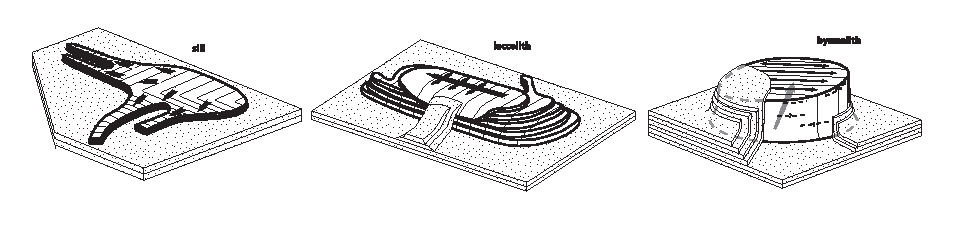
\includegraphics[scale=0.8]{Horsmann.eps}
    \caption{Ces  diagrammes,  réalisés  par  \citet{Horsman:2009gea},
      montrent la structure verticale en  couche de trois intrusions à
      l'érosion  dans les  Henry  mountains. De  gauche  a droite:  le
      Maiden  Creek sill  (Figure \ref{picture}  f), le  Trachyte Mesa
      laccolith et le black mesa bysmalith (Figure \ref{picture} f).}
    \label{Horsmann}
  \end{center}
\end{figure}

\subsection{Intrusion magmatique sur la Lune}
\label{sec:moon}

La densité de la croûte lunaire est particulièrement faible, $2550$ kg
m$^{-3}$ selon  les dernières  estimations faite  à l'aide  des donnés
gravitaires de  la mission GRAIL de  la NASA\citep{Wieczorek:2013ipa}.
La  porosité   résultante  de  4  milliard   d'année  de  bombardement
météoritique, qui  pourrait être  de l'ordre de  $12\%$, ainsi  que la
faible  densité   des  minéraux   la  composant,   principalement  des
plagioclases, tous les  deux contribuent à sa  faible densité. D'autre
part, l'épaisseur  de la croûte  n'est pas négligeable, entre  $34$ et
$43$ km en moyenne  avec une tendance à être plus  épaisse sur la face
cachée que sur la face visible.

La faible  densité de sa crôute  et son épaisseur non  négligeable ont
certainement joué  un rôle  important sur  le volcanisme  lunaire.  En
effet, les  laves extrudés au  sein des  mers lunaires sont  riches en
éléments lourd,  fer principalement  $FeO$ et  titan $TiO_2$,  et sont
caractérisés par  des densités  de l'ordre de  $3000$ kg  m$^{-3}$. La
faible densité de la croûte a donc sans doute jouait aussi sur le Lune
le  rôle d'un  filtre efficace  à l'extrusion  des magmas,  formés par
fusion partielle de son manteau,  en surface, leur flotabilité ne leur
permettant        pas        généralement        d'atteindre        la
surface. \citet{Head:1992bk} ont estimé ainsi à 50 fois plus important
aux volumes  extrudé en surface le  volume des magmas intrusif  sur la
lune.   Cependant, bien  que ce  rapport puisse  donner de  précieuses
indications sur l'évolution thermique de la  lune elle même, il est de
fait très  peu contraints.  La  détection des déformations  de surface
induites par  la mise en  place d'intrusion  magmatique au sein  de la
croûte  permet une  meilleur  caractérisation  du magmatisme  intrusif
lunaire.

Deux  manifestations principales  à  la  surface de  la  lune ont  été
proposé  comme   potentiellement  résultant   de  la  mise   en  place
d'intrusions magmatiques  au sein  de la croûte  lunaire: les  domes à
faible pente et les cratères au sol fracturé.

\begin{itemize}
\item Les  domes à faible pente  sont localisé en bordure  ou dans les
  mers   lunaires,  principalement   sur  la   face  visible   (Figure
  \ref{Moon-magma} a, b).  $13$ de  ces domes ont été recemment décrit
  par \citet{Wohler:2007it}.  Bien que  leur morphologie s'apparente à
  des laccoliths terrestres, ils sont de manière général beaucoup plus
  étalés que  ceux sur  Terre; pour  une même  épaisseur, l'équivalent
  lunaire  peut ainsi  être deux  fois plus  larges que  son homologue
  Terrestre.

  \begin{figure}
    \begin{center}
      \graphicspath{ {/Users/thorey/Documents/These/Manuscript/Figure/Chapter1/} }
      \includegraphics[scale=0.95]{Moon_Lacc.eps}
      \caption{a)  Dome lunaire,  photo  par Appolo  17  b) Apollo  15
        orbital image  AS15-91-12372, vue  oblique du  dôme Valentine.
        c) Cratère au sol fracture Atlas (Classe 1). d) Cratère au sol
        fracturé  Lavoisier (Classe  5).  e)  Cratère au  sol fracturé
        Gassendi  (Classe  3).  f)  Cratère  au  sol fracturé  Komarov
        (Classe   5).   Photo   extraite   de  \textit{Lunar   Orbiter
          Photographic Atlas of the Moon, NASA}}
      \label{Moon-magma}
    \end{center}
  \end{figure}

\item Les  cratères à sol  fracturé sont des cratères  d'impacts ayant
  subis des déformations suite à leur formation.  A peu près $ 200$ de
  ces   cratères  ont   été  répertorié   par  \citet{Schultz:1976kt},
  principalement autour des mers  lunaires (Figure \ref{Moon-magma} c,
  d, e,  f).  La principale  caractéristique de ces cratères  est leur
  faible profondeur  par rapport à  celles des cratères  non déformés.
  En effet, certain  cratère au sol fracturé peuvent  être jusqu'à $2$
  km moins profond que leurs homologues non déformées.  Leur sol, soit
  en  forme de  dôme, soit  plat séparé  des mures  du cratère  par un
  imposant  fossé  circulaire,  est systématiquement  caractérisé  par
  d'important réseaux  de fractures radiales, concentriques  ou encore
  pentagonales (Figure  \ref{Moon-magma} c, d,  e, f).  Basé  sur leur
  profondeur,     topographie     et    niveau     de     déformation,
  \citet{Schultz:1976kt} a postuler l'existence  de six grandes classe
  de  déformation.   La  proximité  des ces  cratères  avec  les  mers
  lunaire, ainsi  que la présence  de produits volcaniques au  sein de
  certain cratère, suggèrent qu'ils ont été déformé suite à la mise en
  place de magma en profondeur sous leur sol.
\end{itemize}

\subsection{Intrusions   magmatiques    sur   les    autres   planètes
  telluriques}
\label{}


\section{Caractérisation du  magmatisme intrusif à  faible profondeur:
  apport de la modélisation}
\label{sec:orign-theor-fram}

\subsection{Model statique de déformation d'une couche élastique}
\label{sec:model-statique-de}

Bien que la  tailles, la morphologie et les volumes  de magmas mise en
jeux peuvent  être récupérés,  à partir  d'observations directs  ou de
méthodes de prospection géophysique sur Terre, ou via les déformations
induites  à  la surface  des  autres  corps  du système  solaire,  ces
informations seuls ne donnent que  peu d'indication sur les mécanismes
de  mise  en  place  de  ces intrusion  magmatiques.   En  effet,  ces
observations  doivent  être interprété  sous  le  regards des  modèles
d'intrusion magmatiques pour pouvoir  extraire des informations sur le
processus d'intrusion lui même, i.e.   sur les paramètres physiques du
magma, les taux d'injection ou encore la profondeur de mise en place.

La propagation  d'un dyke dans un  milieu élastique a été  décrite par
\citep{Lister:1991ut,Rubin:1995upa}.           En         particulier,
\citet{Lister:1990hz} ont montré que, à  l'exeption de la tête du dyke
où  les contraintes  élastiques induites  par les  roches encaissantes
jouent un  rôle important, la dynamique  du magma au sein  du dyke est
contrôlée  par  un  équilibre  entre  la  flotabilité  et  les  pertes
associées à la viscosité du magma lui même. On a vu qu'un dyke peut se
transformer  en sill  si celui  ci  rencontre sa  zone de  flotabilité
neutre. La  dynamique des dykes  et des  sills est comparable  à forte
profondeur   \citep{Lister:1991ut,Cruden:tg},   cependant,  à   faible
profondeur,  la  forme  des  laccoliths supposent  que  les  intrusion
magmatiques se mettent en place principalement par flexion des couches
sédimentaires  sus-jacentes \citep{Johnson:1973ho}.   Les plupart  des
travaux  modélisant  ces  intrusions  magmatiques  utilisent  donc  la
théorie linéaire  de l'élasticité qui  prédit la flexure  d'une plaque
élastique en fonction de la  contrainte appliqué (le taux d'injection)
et     des     caractéristiques     mécaniques     de     l'encaissant
\citep{Pollard:1973ho,Koch:1981if}. Ces travaux  ont par exemple était
appliqué à certain laccolith dans  les Henry Mountains et pour déduire
les  profondeur  d'intrusion et  les  taux  d'injection nécessaire  au
niveau des dômes lunaires \citep{Wohler:2007it} et des cratères au sol
fracturés \citep{Jozwiak:2012dq}.

\subsection{Emplacement dynamics des sills  et laccoliths: que peut on
  apprendre de leur géométrie ?}
\label{sec:empl-dynam-des}

Ces  modèles  statiques  ne  fournissent  aucune  information  sur  la
dynamique du processus d'intrusion et sont donc incapables d'expliquer
la diversité des formes observées. De plus, ils négligent la viscosité
des  magmas ainsi  que  le  propre poids  de  l'intrusion qui  doivent
nécessairement jouer un rôle sur la  mise en place de l'intrusion.  En
l'absence  d'un   modèle  dynamique  d'intrusion,  la   géométrie  des
intrusions répertoriées a été utilisé  pour en déduire des indications
sur les processus de mise en place et de croissance de ces intrusions.
Ainsi,  en utilisant  les donnés  répertoriés sur  les laccoliths  par
\citet{E:2015tl},   \citet{McCaffrey:1997ea}   propose  une   loi   de
puissance empirique pour l'épaisseur  des intrusions $h_0$ en fonction
de leur longueur $R$, $h_0 = bR^a$  ou $a$ est l'exposant de la loi de
puissance et  $b$ une  constante. Ainsi, un  exposant supérieur  à $1$
indique que l'intrusion croit  préférentiellement en s'épaississant et
un  exposant  inférieur  à  $1$   indique  qu'elle  croit  plutôt  par
étalement.

\begin{figure}
  \begin{center}
    \graphicspath{ {/Users/thorey/Documents/These/Manuscript/Figure/Chapter1/} }
    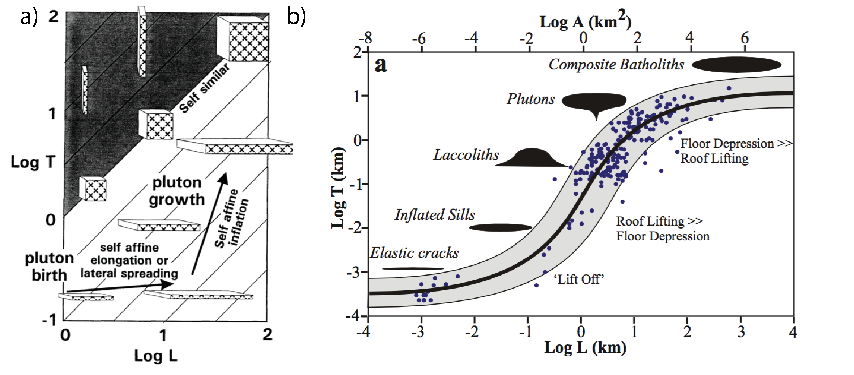
\includegraphics[scale=0.95]{Model.pdf}
    \caption{a)  Schéma de  la formation  des laccoliths  suivant deux
      étapes   par   \citet{McCaffrey:1997ea}.    Nouvelles   données:
      épaisseurs  en  fonction de  leur  longueur  de différent  types
      d'intrusions  magmatiques   à  différentes   locations.   Figure
      extraite de \citet{Cruden:tg}.}
    \label{Model}
  \end{center}
\end{figure}

Les laccoliths  répertoriés par \citep{E:2015tl} montrent  un exposant
$a<1$  ($0.88  \pm 0.1$)  interprété  comme  reflétant l'étalement  de
l'intrusion sur une  certaine distance sous forme d'un  sill avant son
épaississement (Figure  \ref{Model}).  Ce modèle est  cohérent avec le
modèle couramment accepté pour la mise  en place des laccolith en deux
étapes   \citep{Johnson:1973ho,McCaffrey:1997ea}.   Premièrement,   le
magma s'étale latéralement au niveau  de sa zone de flotabilité neutre
$a<1$  jusqu'à ce  qu'un  sill  soit formé  caractérisé  par un  large
rapport  d'aspect.   Ensuite,  lors  de la  deuxième  étape,  le  sill
s'épaissit  par  flexion  des  couches sus-jascentes  pour  former  un
laccolith  caractérisé  par $a>1$  \citep{Johnson:1973ho,Koch:1981if}.
Si la roche sus-jacente est soumise à des contraintes trop importante,
des  failles se  forment au  niveaux  des bords  du sill  et celui  ci
s'épaissit  uniformément sur  toute  sa surface  formant un  bysmalith
\citep{E:2015tl}.   L'étude détaillée  du complexe  intrusif de  l'île
d'Elbe en  Italie (Figure  \ref{Rocchie_Schema}) montre  des exposants
supérieur  à $1$,  jusqu'à $1.5$  interprété comme  étant le  résultat
d'une croissance dominé par l'épaississement de l'intrusion.

Des modèles plus récent conçoivent  plutôt la formation des laccoliths
par empilement successif de sill  de grand rapport d'aspect plutôt que
par  injection   d'un  volume   de  magma  fini   à  un   temps  donné
\citep{Menand:2011ki}.   En effet,  ces  modèles sont  en accord  avec
expérience de \citep{Kavanagh:2006ig}  (Section \ref{sec:stockage}) où
les  sills  se mettent  en  place  à  l'interface entre  deux  couches
rigidité différentes, la rigidité de la couche sus-jascente étant plus
importante que celle de la couche sous-jascente.  En effet, la mise en
place d'un sill en refroidissant  procure un environnement favorable à
la mise en place d'un nouveaux sill,  soit au dessus si la rigidité du
sill solidifié  est inférieur à celle  de la roche sus-jascente  ou en
dessous. Ce modèle  de croissance est supporté par  de récentes études
structurales et  stratigraphiques, notamment au niveau  des intrusions
de     taille    intermédiaires     dans    les     Henry    Mountains
\citep{Horsman:2005ct,Morgan:2008hj,Horsman:2009gea,Menand:2011ki}. Ce
modèle permet aussi de rendre compte de la structure plate du toit des
laccoliths.   Cependant, ce  mécanisme  de croissance  ne devrait  pas
impliquer  un   exposant  caractéristique  de  la   géométrie  de  ces
laccoliths.

\citet{Nachwuchskoechin:2002tv}  ont réunit  des donnés  sur une  plus
grande plage  de longueurs,  des petits  cracks élastique  de quelques
dizaines de mètres aux battholith  de quelques centaines de kilomètres
(Figure  \ref{Model}).  \citep{Nachwuchskoechin:2002tv}  proposent que
l'épaisseur en fonction de la longeur des intrusions magmatiques forme
une   distribution  en   forme  de   sigmoide  (   dans  une   échelle
logarithmique) avec  une pente  maximum de $1.5$  caractéristiques des
laccoliths.   Cependant, aucune  théorie sous-jascente  soutient cette
observation. De plus, les données  de \citep{Cruden:tg} sur les larges
sills   mafiques   contredise   cette  vision   des   choses   (Figure
\ref{Dimension}).

\section{Discussion}
\label{sec:discussion}

En conclusion, aucun des modèles  présentés plus haut n'est cohérent à
la  fois avec  la morphologie  des sills  et des  laccoliths et  leurs
rapport  d'aspect.  Dans  le  but  de comprendre  plus  en détails  la
dynamique de l'intrusion, \citet{Michaut:2011kg} a développé un modèle
théorique d'étalement  d'un magma  visqueux sous une  couche élastique
d'épaisseur contant continuellement nourrit par un conduit vertical en
son centre. Ce  modèle diffère de ces prédecesseurs par  sa capacité a
traité la  dynamique même de l'intrusion  ainsi que le poids  du magma
comme un moteur  de l'écoulement. Ce modèle a été  développé en 2D par
\citep{Thorey:2014cv}. Dans  la suite,  je présente  le modèle  et les
résultats que nous avons obtenus dans une géométrie axisymmétrique.


\bibliographystyle{agufull08}
\bibliography{/Users/thorey/Dropbox/Library}

%%% Local Variables:
%%% mode: latex
%%% TeX-master: "../main"
%%% End:

\chapter{Isoviscous elastic-plated  gravity current model  for shallow
  magmatic intrusion}

\label{chap2} 
\minitoc

\citet{Michaut:2011kg} proposed  a new  model for  the spreading  of a
shallow   depth   intermediate-size   intrusions,   where   magma   is
continuously injected at the center and is accommodated by the bending
of  the  overlying strata.   In  particular,  the model  differs  from
previous ones by  considering the dynamics of  the emplacement itself,
in a  sense that the  radius in self-consistently determined,  and the
driving  force  associated  with  the magma  weight  which  were  both
neglected   in   older   models.    In   the   original   paper   from
\citet{Michaut:2011kg}, the  model was  derived in both  cartesian and
axisymmetric geometry and the results  were presented in 2D. A similar
model in $2D$ with an additional  fracture criterion at the tip of the
intrusion    has   been    derived   by    \citet{Bunger:2011cb}   and
\citet{Anonymous:QWXp_4JV}  discussed precisely  the  dynamics at  the
contact  line  and  the  case of  an  elastic-plated  gravity  current
spreading over an inclined  plane \citep{Anonymous:QWXp_4JV}.  In this
chapter, we  present a summary  of the model  and the results  for the
spreading of an isoviscous elastic-plated gravity current over a rigid
horizontal  surface in  an axisymmetrical  geometry.  Results  in this
geometry  have been  thoroughly studied  by \citet{Lister:2013ia}  and
this model will constitute the  reference for more elaborate models in
the manuscript.

\section{Model}
\label{C2-sec:model}

The model considers an isoviscous elastic-plated gravity current, i.e.
an  isoviscous  fluid  of  viscosity  $\eta_h$  and  density  $\rho_m$
spreading beneath a thin elastic sheet  of thickness $d_c$ and above a
semi infinite rigid layer \citep{Michaut:2011kg,Bunger:2011cb} (Figure
\ref{C2-Sketch}).  The fluid is injected  continuously at the base and
center of the current at a rate $Q_0$ through a cylindrical conduit of
diameter $a$.

\begin{figure}[htbp]
  \begin{center}
    \graphicspath{ {/Users/thorey/Documents/These/Manuscript/Figure/Chapter2/} }
    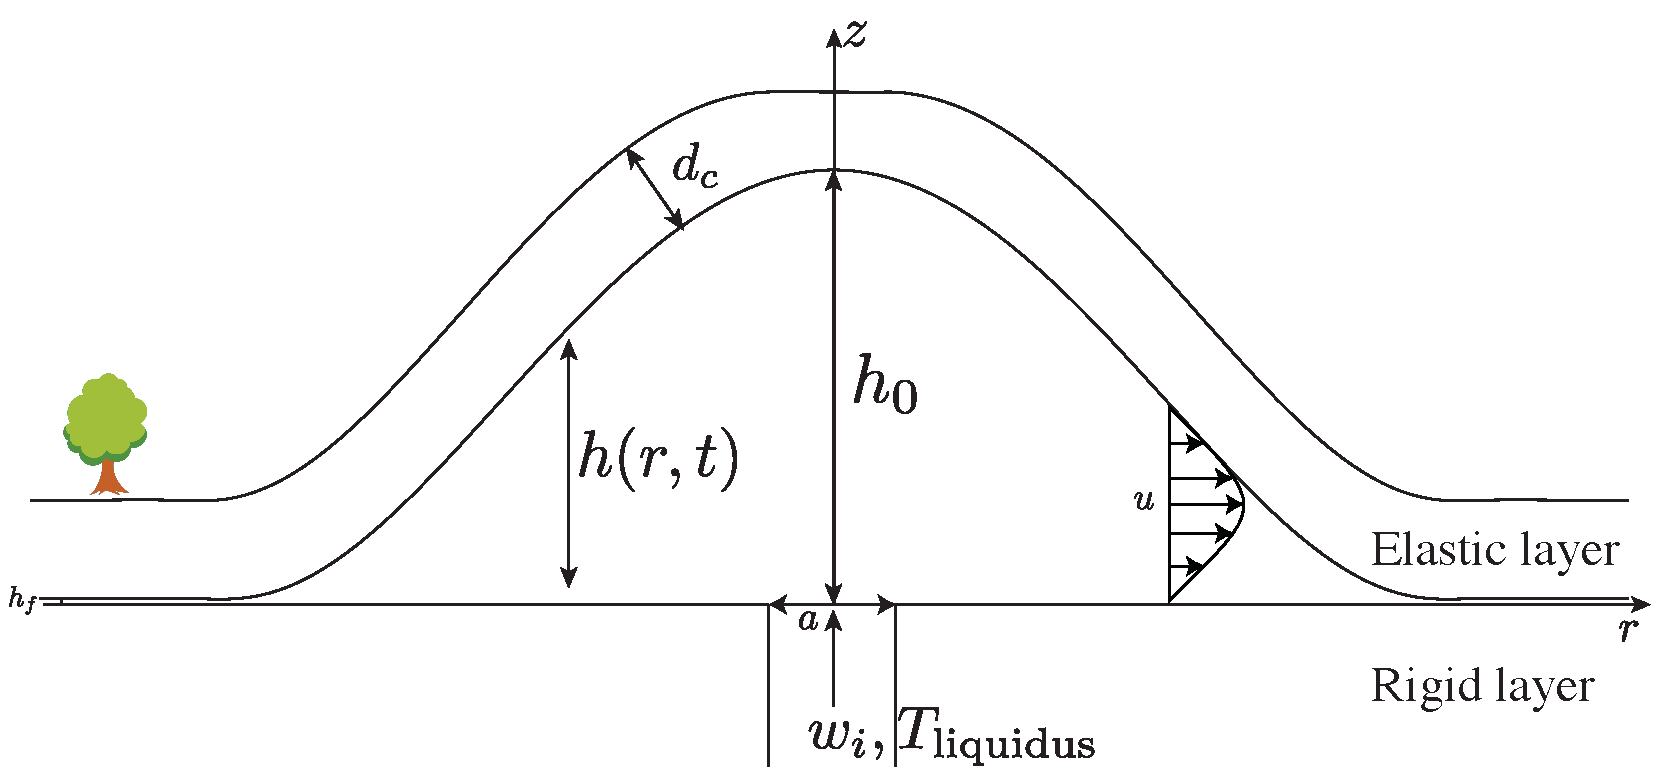
\includegraphics[scale=0.40]{C2_Sketch.pdf}
    \caption{Model geometry and parameters.}
    \label{C2-Sketch}
  \end{center}
\end{figure}

\subsection{Governing equation}
\label{C2-sec:Governing equation}

\textbf{Driving pressure}\\

The  intrusion develops  over a  length scale  $\Lambda$ that  is much
larger than its  thickness $H$ ($\epsilon = H/ \Lambda<<  1$).  In the
laminar  regime  and  in  axisymmetrical  coordinates  ($r$,$z$),  the
Navier-stokes equations within the lubrication assumption are
\begin{eqnarray}
  -\frac{\partial P}{\partial r}  +  \frac{\partial}{\partial z}\left(\eta \frac{\partial u}{\partial z}\right) &=&0\label{C2_V1} \\
  -\frac{\partial P}{\partial z}  - \rho_{m}g&  =&0\label{C2-Npressure}
\end{eqnarray}
where  $u(r,z,t)$  is  the  radial   velocity,  $g$  is  the  standard
acceleration due to gravity and  $P(r,z,t)$ is the pressure within the
fluid.   Integration  of  (\ref{C2-Npressure}) thus  gives  the  total
pressure  $P(r,z,t)$ within  the flow.   When the  vertical deflection
deflection $h(r,t)$  of the upper  elastic layer is small  compared to
its thickness  $d_c$, i.e $h<<d_c$,  we can neglect stretching  of the
upper layer and only consider  bending stresses.  Therefore, the total
pressure $P(r,z,t)$ at a level $z$ in the intrusion is the sum of four
contributions: the  weight of the  magma and  of the upper  layer, the
bending pressure $P_b$ and the atmospheric pressure $P_0$
\begin{equation}
  P = \rho_m g (h-z)+\rho_rgd_c+P_b+P_0
  \label{C2-pression}
\end{equation}
where $h(r,t)$ is the intrusion  thickness and $\rho_r$ the density of
the surrounding rocks. The bending pressure  is given by the force per
unit area  that is necessary  for a  vertical displacement $h$  of the
thin elastic plate \citep{Turcotte:1982ca}
\begin{equation}
  P_d = D\nabla^4h
\end{equation}
where $D$  is the flexural  rigidity of  the thin elastic  layer, that
depends on the Young's modulus $E$, Poisson's ratio $\nu^*$ and on the
elastic           layer          thickness           $d_c$          as
$D = Ed_c^3/\left(12(1-\nu^*)\right)$.

\vspace{.5cm} \textbf{Velocity field} \vspace{.5cm}

At the contact with the elastic sheet $z=h(r,t)$, the no-slip boundary
condition is present  and so, the tangential velocity is  zero and the
normal velocity  is the change  in height ($\partial h/  \partial t$).
With $\vec{n}$ the normal to the surface and $\vec{t}$ the tangent, we
have
\begin{eqnarray}
  \vec{n} \cdot (u,w) &=& \frac{\partial h }{\partial t}\\
  \vec{t} \cdot (u,w) &=& 0 \label{tangeant}.
\end{eqnarray}
The  tangent  vector is  $\vec{t}  =  (1,  \partial h/  \partial  r)$.
However, within the lubrication  assumption, the vertical component of
the  tangent  vector scales  as  $\epsilon$  and thus,  is  negligible
compared to  the radial  component. Therefore, the  boundary condition
($\ref{tangeant}$) reduces  to $u(r,z=h,t)  =0$.  At  the base  of the
flow, the same boundary condition hold and $u(r,z=0,t) =0$.

Equation (\ref{C2_V1}) is integrated twice  as a function of $z$ using
these boundary conditions and the horizontal velocity is
\begin{equation}
  u(r,z,t) =\frac{1}{2\eta} \frac{\partial P}{\partial r} \left(z^2-hz\right)
  \label{C2-vel}
\end{equation}

\vspace{.5cm} \textbf{Injection rate} \vspace{.5cm}

The effective overpressure $\Delta P^*$ driving the flow in the feeder
conduit decreases as the intrusion thickens and is given by
\begin{equation}
  \Delta P^* = \Delta P -\rho_m g h_0 \label{C2-Q0}
\end{equation}
where $h_0(t)$ is the maximum  intrusion thickness at the center $r=0$
and $\Delta P$ is the initial  driving pressure or the overpressure at
the base of the dyke ($z = -Z_c$).

In (\ref{C2-Q0}), the bending pressure  at then center, which scale as
D$h_0(t)/R(t)^4$  where  $R(t)$  is   the  blister  radius,  has  been
neglected.  Although  it tends  to infinity at  the initiation  of the
flow, it rapidly  vanishes as the blister spreads  and the hydrostatic
pressure $\rho_m g h_0$ becomes  the main contribution to the pressure
at the  center.  In addition, the  model assumes a large  aspect ratio
for the blister and does not consider the initiation of the flow.

Finally,  assuming a  Poiseuille flow  within the  cylindrical feeding
conduit, the vertical injection velocity $w_i(r,t)$ and injection rate
$Q(t)$ are given by
\begin{equation}
  w_i=
  \begin{cases}
    \frac{ \Delta P^*}{4 \mu Z_{c}} (\frac{a^{2}}{4}-r^{2})& r \le \frac{a}{2}\\
    0 & r > \frac{a}{2}
  \end{cases}
  \label{C2-eq12}
\end{equation}
\begin{equation}
  Q = Q_0(1-\frac{\rho_m g h_0}{\Delta P})
  \label{C2-eq11}
\end{equation}
where
$Q_0=\left(\pi \Delta P^* a^{4}\right)/\left(128 \eta Z_c\right)$.

\vspace{.5cm} \textbf{Mass conservation} \vspace{.5cm}

The fluid  is assumed  incompressible and a  global statement  of mass
conservation gives
\begin{eqnarray}
  \frac{\partial         h}{\partial        t} +\frac{1}{r}
  \frac{\partial}{\partial
  r} \left( r\int_0^hudz\right) = w_i
  \label{C2-Mass}
\end{eqnarray}
and using (\ref{C2-vel}), we find  that the equation for the evolution
of the thickness in time and space reads
\begin{equation}
  \frac{\partial h}{\partial t} =\frac{\rho_mg}{12 \eta r}
  \frac{\partial}{\partial r}  \left( rh^3  \frac{\partial h}{\partial
      r}\right)+\frac{D}{12\eta r} \left( rh^3 \frac{\partial}{\partial r}\nabla^4h\right)+
  w_i .\label{C2-Heq}
\end{equation}
It is  composed of three different  terms on the right  hand side. The
first term represents gravitational  spreading, i.e.  spreading of the
blister under its own weight. The second term represents the squeezing
of the  flow by the upper  elastic layer.  Both term  are negative and
induces spreading.   The last term  represents fluid injection  and is
positive.

\subsection{Dimensionless equations}
\label{C2-sec:dimens-equat}

Equations  (\ref{C2-eq12}) and  (\ref{C2-Heq}) are  nondimensionalized
using a  horizontal scale $\Lambda$, a  vertical scale $H$ and  a time
scale $\tau$ given by
\begin{eqnarray}
  \Lambda &=& \left(\frac{D}{\rho_m g}\right)^{1/4}\label{L1}\\
  H&=&\left       (\frac{12\eta      Q_{0}}{\rho_{m}g       \pi}\right      )
       ^{\frac{1}{4}} \label{H1}\\
  \tau&=&\frac{\pi \Lambda^{2} H}{Q_{0}}\label{T1}
\end{eqnarray}

where scales  are chosen  such that $Q_0  = \pi\Lambda^2  H/\tau$. The
length scale $\Lamba$ represents the  flexural wavelength of the upper
elastic layer,  i.e. the  length scale at  which bending  stresses and
gravity  contributes equally  to flow.   The height  scale $H$  is the
thickness of  a typical gravity current  and the time scale  $\tau$ is
the  characteristic time  to  fill  up a  cylindrical  flow of  radius
$\Lambda$ and thickness  $H$ at constant rate $Q_0$.   In addition, we
can       define        a       horizontal        velocity       scale
$U=\Lambda/\tau=\left(\rho_m           g           H^3\right)/\left(12
  \eta_h\Lambda\right)$.

The dimensionless equation is
\begin{eqnarray}
  \frac{\partial h}{\partial t}& =&\frac{1}{ r}
                                    \frac{\partial}{\partial r}  \left( rh^3  \frac{\partial h}{\partial
                                    r}\right)+\frac{1}{ r} \left( rh^3
                                    \frac{\partial}{\partial
                                    r}\nabla^4h\right)\nonumber\\
                               &+&
                                   \frac{32}{\gamma^{2}}\left(\frac{1}{4}-\frac{r^{2}}{\gamma^{2}}\right)\left(1-\frac{h_0}{\sigma}\right)
                                   \label{C2-mainEq}
\end{eqnarray}
where the last term is replaced by zero for $r>\gamma/2$. $\gamma$ and
$\sigma$ are  two dimensionless numbers  that control the  dynamics of
the flow
\begin{eqnarray}
  \gamma &=& \frac{a}{\Lambda}\\
  \sigma &=& \frac{\Delta P}{\rho_m g h}.
\end{eqnarray}
$\gamma$  is the  dimensionless radius  of  the conduit,  it does  not
significantly influence the flow and is set to $0.02$ in the following
\citep{Michaut:2009jx,Michaut:2011kg}.   $\sigma$  is  the  normalized
pressure  head,  i.e.,  the  ratio between  the  initial  overpressure
driving the flow and the weight of the magma at the center.
	 
\subsection{Need for regularization}
\label{C2-sec:need-regularization}

One  of   the  main   mathematical  difficulty  in   solving  equation
(\ref{C2-mainEq}) arises at the  contact line.  Indeed, the assumption
that the  thickness of  the fluid  tends to zero  at the  contact line
leads       to       divergent      viscous       stresses,       i.e.
$\eta  \partial   u/\partial  z\rightarrow  \infty$  and   hence,  the
theoretical         immobility          of         the         blister
\citep{Flitton:1999iv,Lister:2013ia,Anonymous:QWXp_4JV}. This problem,
known  a  the  contact-line  paradox,  is  a  well  know  problem  for
surface-tension driven flow  such as the spreading of  a water droplet
\citep{Bertozzi:1998wz,Snoeijer:2013cm}.

The formal proof  have been derived by  \citet{Flitton:1999iv} and can
be derived  as follow. Suppose  that (\ref{C2-mainEq}) has  a solution
and the solution has the  form $h \sim A(t)(R(t)-r)^{\alpha}$ near the
contact line.  As $r \rightarrow R(r)$, the bending term dominates the
gravitational term and (\ref{C2-mainEq}) reduces to
\begin{eqnarray}
  \frac{\partial       h}{\partial       t}&      =&\frac{1}{       r}
                                                     \frac{\partial}{\partial r}\left( rh^3 \frac{\partial}{\partial r}\nabla^4h\right).
                                                     \label{C2-mainEq2}
\end{eqnarray}
Injecting the  solution into  (\ref{C2-mainEq2}) and keeping  only the
leading powers of $R-r$ gives
\begin{eqnarray}
  \frac{\partial    R}{\partial    t}    A\alpha\left(R-r\right)^{\alpha-1}+
  \frac{\partial           A}{\partial           t}\left(R-r)^{\alpha}
  &=&A^4\alpha(\alpha-1)(\alpha-2)\nonumber\\
  &&(\alpha-3)(\alpha-4)(\alpha-5)(R-r)^{4\alpha-6}\nonumber
\end{eqnarray}
The time derivative is locally dominated by its convective part at the
tip, the second  term on the left  is small compared to  the first and
therefore,   by   equating   the   exponent  of   $R-r$,   we   obtain
$\alpha = 5/3$, and by equating the coefficients, we deduce
\begin{equation}
  \frac{\partial R}{\partial r} =-\frac{280}{243} A^3.
\end{equation}
It shows that (\ref{C2-mainEq}) can  only have retreating contact line
($dR/dt<0$)   but  not   with  advancing   contact  line   ($dR/dt>0$)
\citep{Lister:2013ia,Flitton:1999iv}.

To  mitigate this  problem,  one  common approach  is  to  add a  thin
prewetting film, with thickness $h_f$ such that $h\rightarrow h_f$ as
$r\rightarrow  \infty$.   While  the  solution will  depend  upon  the
prewetting  film thickness  $h_f$ and  will not  show any  convergence
properties when $h_f\rightarrow 0$, we will see that the dependence in
$h_f$ is  weak and the  difference between different values  for $h_f$
will  be  relatively  small  \citep{Lister:2013ia,Anonymous:QWXp_4JV}.
Unless otherwise specified, we will consider $h_f = 5\cdot 10^{-3}$ in
the manuscript.



\section{Results}
\label{C2-sec:regime-propagations}

For  a  small  prewetting   film  thickness,  i.e.   $h_f/H<<1$,  the
numerical  resolution of  the  equation  (\ref{EqFinal1}) shows  three
spreading regimes:  a bending  regime where  gravity is  negligible, a
viscous  gravity current  regime  where bending  is  negligible and  a
regime               of              lateral               propagation
\citep{Michaut:2011kg,Bunger:2011cb,Lister:2013ia}.

\begin{figure}[h!]
  \begin{center}
    \graphicspath{ {/Users/thorey/Documents/These/Manuscript/Figure/Chapter2/} }
    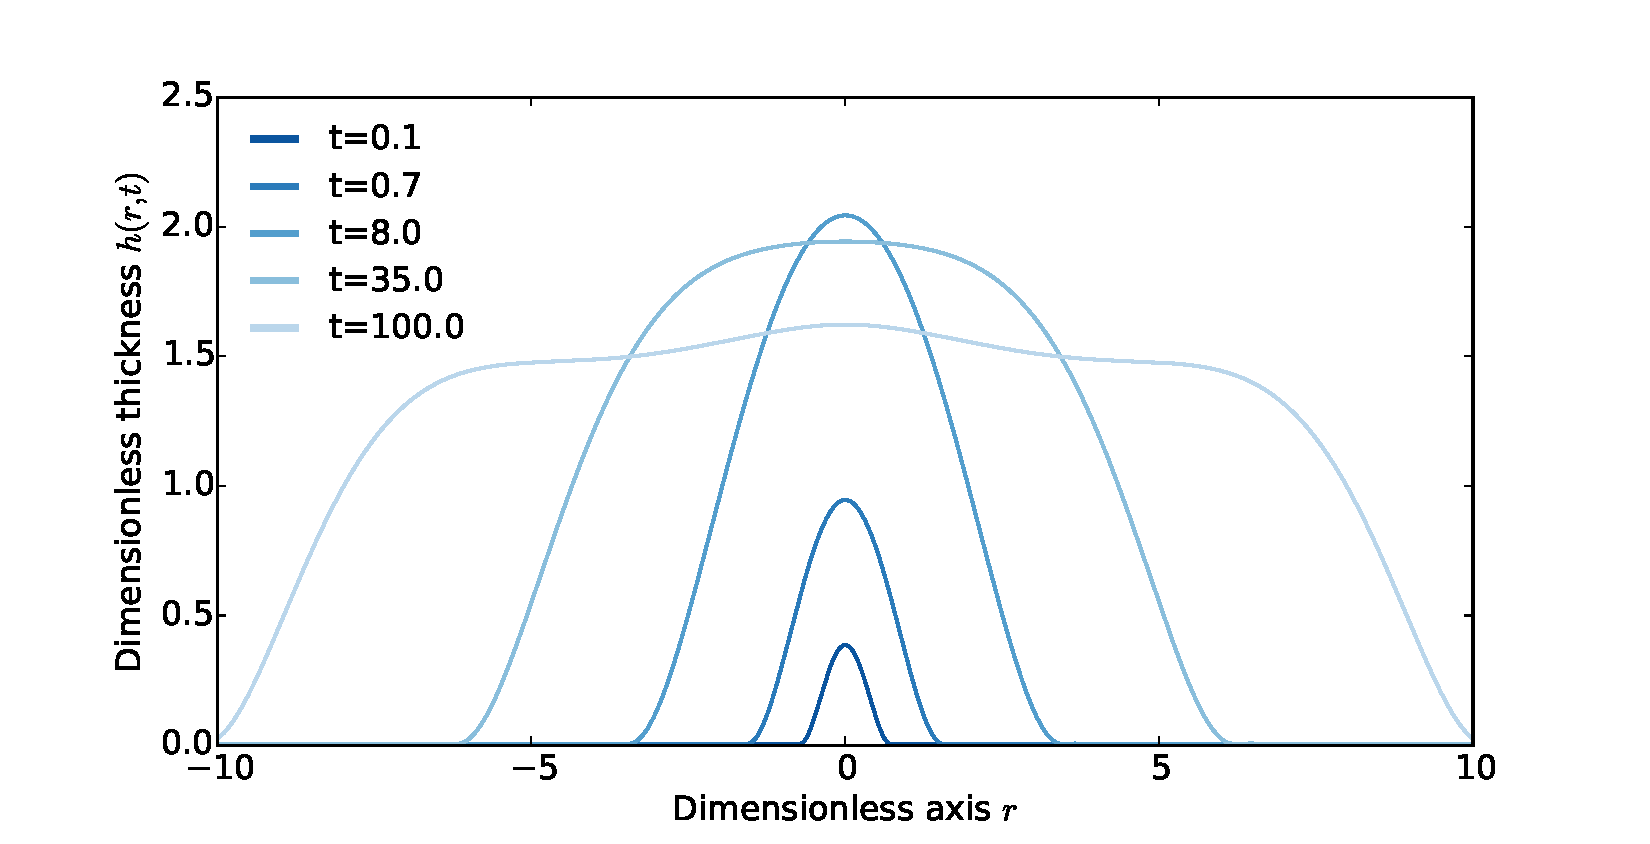
\includegraphics[scale=0.5]{C2_ELAS_GRAV_Profil.eps}
    \caption{Shape of the flow, i.e.  thickness $h(r,t)$ as a function
      of the radial axis $r$ at  five different times indicated on the
      plot. Variables are  dimensionless and one needs  to multiply by
      the characteristic  scales (thickness,  length or time  given by
      (\ref{H1}),  (\ref{L1})  or  (\ref{T1})) to  obtain  dimensional
      values.   For $t<10$,  the intrusion  is in  the bending  regime
      whereas  for $t>10$  the  intrusion is  in  the gravity  current
      regime.}
    \label{C2_ELAS_GRAV_Profil}
  \end{center}
\end{figure}

\subsection{Bending regime}
\label{C2-sec:bending-regime}

At  early times,  when  $R<<\Lambda$, gravity  is  negligible and  the
dynamics of  the spreading  is governed  by the  bending of  the upper
layer.   In addition,  if $h_0<<\sigma$,  the overpressure  $\Delta P$
driving the flow is much larger than  the weight of the blister at the
center and the injection rate can be considered constant.

In that case, the spreading is  very slow and the interior has uniform
pressure $P =\nabla^4h$.  The flow is bell-shaped and its thickness is
given by
\begin{equation}
  h(r,t) = h_0(t)\left(1-\frac{r^2}{R^2(t)}\right)^2
  \label{IntrusionShape}
\end{equation}
with  $h_0(t)$   the  thickness  of   the  intrusion  at   the  center
\citep{Michaut:2011kg,Lister:2013ia}.       In       this      regime,
\citet{Lister:2013ia} have  shown that the spreading  is controlled by
the propagation  of a peeling by  bending wave at the  intrusion front
with dimensionless velocity $c$
\begin{equation}
  c=    \frac{\partial             R}{\partial            t}             =h_f^{1/2}
  \left(\frac{\kappa}{1.35}\right)^{5/2}
  \label{WaveVelocity}
\end{equation}
where  $\kappa  =  \partial^2  h/\partial r^2$  is  the  dimensionless
curvature  of  the  interior  solution.   Using  the  propagation  law
(\ref{WaveVelocity})   and  the   form   of   the  interior   solution
(\ref{IntrusionShape}), they  find that the  radius and the  height of
the intrusion are given by similarity solutions
\begin{eqnarray}
  R(t) &=& 2.2h_f^{1/22}t^{7/22}\label{ScalingR}\\
  h_0(t)&=&0.7 h_f^{-1/11}t^{8/22}\label{ScalingH}.
\end{eqnarray}
where the numerical pre-factor have been matched to our simulations.

\begin{figure}
  \begin{center}
    \graphicspath{ {/Users/thorey/Documents/These/Manuscript/Figure/Chapter2/} }
    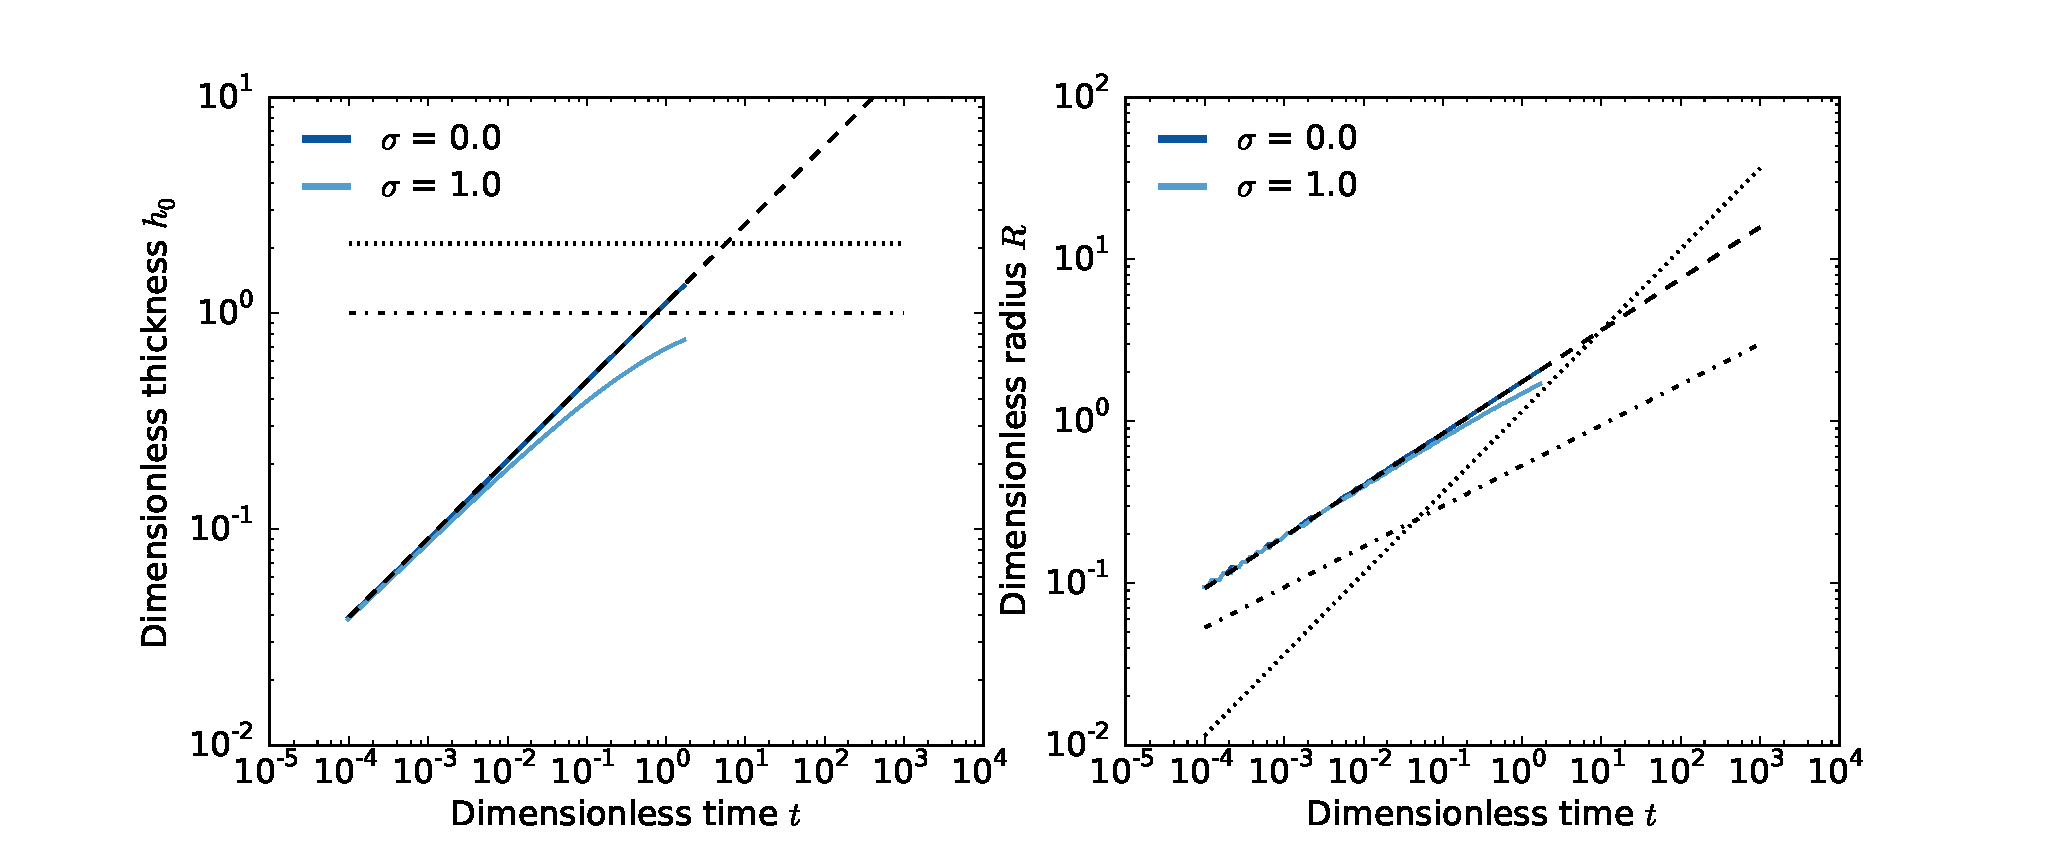
\includegraphics[scale=0.4]{C2_ELAS_GRAV_Sigma.eps}
    \caption{Left: Dimensionless thickness at  the center $h_0$ versus
      dimensionless  time  $t$   for  different  dimensionless  number
      $\sigma$  indicated on  the  plot.   Dashed-lines represent  the
      scaling  laws in  the different  regimes.  Right:  Dimensionless
      radius  $R$   versus  dimensionless   time  $t$  for   the  same
      dimensionless  number  $\sigma$.    Dashed-lines  represent  the
      scaling laws in the different regimes.}
    \label{C2_ELAS_GRAV_Sigma}
  \end{center}
\end{figure}

\subsection{Gravity current regime}
\label{C2-sec:grav-curr-regime}

In  contrast, when  the radius  R becomes  much larger  than $\Lambda$
($R>>\Lambda$), the weight of the  intrusion becomes dominant over the
bending  terms.  The  pressure is  given by  the hydrostatic  pressure
$P = h$  and the intrusion enters a classical  viscous gravity current
regime where bending terms only affect the solution near the intrusion
edge   \citep{Huppert:1982a,Michaut:2011kg,Lister:2013ia}.   In   this
second regime, the radius evolves as $t^{1/2}$ and the thickness tends
to a constant
\begin{eqnarray}
  R(t) &=& 0.715 t^{1/2}\label{Scaling-R-Gravi}\\
  h_0 &=& 1.86\label{Scaling-H-Gravi}
\end{eqnarray} 

\subsection{Lateral propagation}
\label{sec:lateral-propagation}

Once $h_0\rightarrow \sigma$,  the flow is thick  enough to compensate
for  the initial  overpressure. The  thickness at  the center  remains
constant and  the flow enters  a regime of lateral  propagation, where
only its radius $R(t)$ is  to increase \citep{Michaut:2011kg}. In this
regime, except at the center when it redistributes the pressure over a
length scale $\Lambda$, the bending term is negligible compared to the
gravitational  term. \citet{Michaut:2011kg}  has  shown  that in  this
regime, the thickness is constant and the radius evolves as $t^{1/4}$
\begin{eqnarray}
  R(t) &=& \left(\frac{\sigma^3 t}{4\pi}\right)^{1/4}\label{Scaling-R-Propa}\\
  h_0 &=& \sigma\label{Scaling-H-Propa}
\end{eqnarray} 

\section{Application to laccoliths}
\label{C2-sec:appl-earth-moon}

\subsection{Range of value for the parameters}
\label{sec:range-value-param}

In terrestrial settings,  lava density $\rho_m$ depends  mainly on its
composition and varies between $ 2300$ kg m$^{-3}$ for felsic lavas to
$3000$ kg m$^{-3}$ for mafic  lavas. Hence, for Young's modulus values
between $10$ and $100$ GPa and  intrusion depths between $0.1$ and $5$
km, the characteristic  length scale $\Lambda$ varies  between $1$ and
$10$  km.   The overpressure  in  magma  reservoirs driving  dykes  is
typically    between    a    few    to    several    tens    of    MPa
\citep{Tait:1988vn,Marti:2000fe} and  the conduit length  $Z_c$ varies
from a few  to several tens of kilometers. Lava  viscosity at eruption
temperature  $\eta_h$  depends mainly  on  its  composition and  water
content; close to its liquidus temperature,  it can varies from $1$ Pa
s  for   ultramafic  lavas   to  $10^{6}$  Pa   s  for   felsic  lavas
\citep{Anonymous:CZVBrBvv,Giordano:2008em,Whittington:2009fv,Chevrel:2013jn}.
Hence,  injection  rate  $Q_0$  are in  a  range  $10^{-3}-0.1$  m$^3$
s$^{-1}$ and  the height scale  $H$ varies  between $0.1$ m  for mafic
lavas to  $1$ m for  felsic lavas.   Therefore, the time  scale $\tau$
varies  from a  few months  for mafic  lavas to  few years  for felsic
lavas.

\begin{figure}
  \begin{center}
    \graphicspath{ {/Users/teihorey/Documents/These/Manuscript/Figure/Chapter2/} }
    \includegraphics[scale=0.35]{C2_Geological_Data.eps}
    \caption{}
    \label{C2_Geological_Data}
  \end{center}
\end{figure}

\subsection{Earth : Observation Vs Prediction}
\label{sec:observ-vs-pred}

\vspace{.5cm} \textbf{Dataset} \vspace{.5cm}

\citet{E:2015tl} have  made an  extensive catalog of  $900$ laccoliths
across  the  world.   In   particular,  \citet{E:2015tl}  provide  the
thickness and  the radius  of $168$ laccoliths  among which,  $40$ are
also  provided  with  an  estimation  of  the  intrusion  depth.   The
thickness  ranges from  $100$  meters  to $10$  km  and, although  the
largest one goes up to $100$ km, their radius mostly range form $1$ to
$10$  km.  While  most of  the data  are located  in the  United State
($\sim 90\%$), the different laccoliths are widely spread among on the
territory and variation in the parameters between different laccoliths
is most  likely to be  important. Therefore,  in addition to  the data
from  \citet{E:2015tl},  we  also  consider in  this  study  the  data
provided by \citet{Rocchi:2002jy} on $9$ laccoliths nested in the same
christmas tree structure. For this  dataset, each laccolith is part of
a  larger  intrusive  system,  and  hence  variability  of  the  model
parameters should be  limited, except for the  overlying elastic layer
thickness, taken  to be the  intrusion depth, whose  variation between
laccoliths is  given by \citet{Rocchi:2002jy}. Indeed,  the dispersion
is much smaller  for this dataset, the radius ranges  from $1$ to $10$
km and the thickness from $40$m to $1$ km. In order to account for the
intrinsic scale of different settings for each intrusion, the data are
first   nondimensionalized  using   characteristic   values  for   the
parameters and the intrusion depth, when known, for the data.

\begin{figure}
  \begin{center}
    \graphicspath{ {/Users/thorey/Documents/These/Projet/Refroidissement/Skin_Model/Figure/Figure_Data/} }
    \includegraphics[scale=0.42]{Corry_Rocchie.eps}
    \caption{Left: Thickness $h_0$  (m) versus the radius  $R$ (m) for
      laccoliths   reported   by    \citet{E:2015tl}   in   blue   and
      \citet{Rocchi:2002jy} in red.  Right: Dimensionless thickness as
      a  function of  dimensionless radius,  characteristic thickness,
      and  length  are  calculated  from  (\ref{H1})  and  (\ref{L1}).
      Dashed lines: predicted scaling law from the simulations (black)
      and  best fit  for the  power  law $h_0=aR^b$  for each  dataset
      obtained from a linear least-square regression in log-log space.
      I  use  for the  parameters,  $g=9.81$  m s$^{-2}$,  $Q_0=  0.1$
      m$^{3}$  s$^{-1}$, $\rho_m=2500$  kg  m$^{-3}$,  $E=10$ GPa  and
      $\eta_h=10^6$ Pa s.  Unless the intrusion depth is  given by the
      dataset, we use $d_c=1500$ m and $\nu^*=0.25$.}
    \label{Corry_Rocchie}
  \end{center}
\end{figure}



\vspace{.5cm} \textbf{Range of value for the parameters} \vspace{.5cm}

In terrestrial settings,  lava density $\rho_m$ depends  mainly on its
composition and varies between $ 2300$ kg m$^{-3}$ for felsic lavas to
$3000$ kg m$^{-3}$ for mafic  lavas. Hence, for Young's modulus values
between $10$ and $100$ GPa and  intrusion depths between $0.1$ and $5$
km, the characteristic  length scale $\Lambda$ varies  between $1$ and
$10$  km.   The overpressure  in  magma  reservoirs driving  dykes  is
typically    between    a    few    to    several    tens    of    MPa
\citep{Tait:1988vn,Marti:2000fe} and  the conduit length  $Z_c$ varies
from a few  to several tens of kilometers. Lava  viscosity at eruption
temperature  $\eta_h$  depends mainly  on  its  composition and  water
content; close to its liquidus temperature,  it can varies from $1$ Pa
s  for   ultramafic  lavas   to  $10^{5}$  Pa   s  for   felsic  lavas
\citep{Anonymous:CZVBrBvv,Giordano:2008em,Whittington:2009fv,Chevrel:2013jn}.
Hence,  injection  rate  $Q_0$  are in  a  range  $10^{-3}-0.1$  m$^3$
s$^{-1}$ and  the height scale  $H$ varies  between $0.1$ m  for mafic
lavas to  $1$ m for  felsic lavas.   Therefore, the time  scale $\tau$
varies  from a  few months  for mafic  lavas to  few years  for felsic
lavas.

The model  also considers  a thin pre-wetted  film of  thickness $h_f$
whose  meaning in  the application  to the  spreading of  laccolith is
unclear.  In  particular, the  model shows  no convergence  when $h_f$
tends to zero \citep{Lister:2013ia} and therefore, the thickness $h_f$
might be  linked to some structural  length scale at the  front of the
laccolith or  to the natural  imperfection of the flow  geometry.  For
the purpose of the application, we  choose a film thickness of $1$ mm,
i.e.  the  minimum length  scale with  physical signification  for the
spreading of laccoliths  which give a dimensionless  $h_f$ that varies
between $10^{-2}$ and $10^{-4}$.  The limited effect of changing $h_f$
is detailed in  Appendix \ref{FilmThickness} and in  the following, we
set $h_f$ to $10^{-3}$.

\vspace{.5cm} \textbf{Comparison with the model} \vspace{.5cm}

Using these depths and characteristic values for various properties of
the system, the length and thickness  scales can be estimated for each
laccolith  such   that  the   data  can  be   nondimensionalized.   To
characterize  the mean  trend in  each population,  we make  use of  a
linear least-square regression in log-log  space to obtain a power law
relationship  of the  form $h_0=aR^b$  as predicted  by the  model and
\citet{McCaffrey:1997ea}.  We found $h_0=170 R^{0.63\pm 0.08}$ for the
laccolith of Corry and $h_0=135 R^{1.21\pm 0.1}$ for the laccoliths at
Elba Island.

The model evolution of the radius $R$  of the current as a function of
its thickness can be easily derived from thickness $h_0$ as a function
of its radius $R$ for a current  that solidifies in the third phase of
the   bending  regime   can   be  derived   from   the  scaling   laws
(\ref{ScalingH}) and (\ref{ScalingR}) and should follow
\begin{equation}
  h_0 \sim 0.75 R^{8/7}\label{Hr}
\end{equation}

For the laccolith  system at Elbas Island, the  best fit dimensionless
thickness  for  $h_0$ is  proportional  to  $R^{1.21}$, a  little  bit
smaller than  the model  prediction. \citep{Michaut:2011kg}  founds in
$2D$ that  $R^{1.25}$, The  geometry of these  laccoliths is  not well
known  and probably  not  perfectly two‐dimensional  or circular,  the
value nicely insert between the  two. The dimensionless radius is also
smaller   than   $4$   supporting   their  arrest   in   the   bending
regime. However, the model prefactor is not explain b

\section{Discussion}
\label{C2-sec:discussion}

\begin{table}
  \caption{Range of values for the model parameters}
  \centering
  \begin{tabular}{c|c|c|c|c}
    Parameters& Symbol & Earth & Moon&Unit\\
    \hline
    &&&&\\
    Depth of intrusion & $d_c$ & $0.1-5$ &$0.1-5$ &km \\
    Young's Modulus & $E$ & $10-100$ &$10-100$ &GPa \\
    Poisson's ratio & $\nu^*$ & $0.25$ &$0.25$ &\\
    Gravity & $g$ & $9.81$ &1.62&m s$^{-2}$ \\
    Crust density & $\rho_{r}$ & $2500$ &$2500$&kg m$^{-3}$ \\
    Magma density & $\rho_{m}$ & $2500-3000$ &$3000$&kg m$^{-3}$ \\
    Magma viscosity & $\eta_h $ & $1-10^{4}$ &$1-10^{2}$&Pa s \\
    Feeder dyke width & $a$ & $1-100$ &$1-10$&m \\
    Depth of the melt source & $Z_{c}$ & $ 1-10$&$200-500$& km \\ 
    Initial overpressure & $\Delta P$ & $5-50$ &$1-5$ &MPa \\
    Injection rate & $Q_{0}$ &$0.01-1$ &$1-10$&m$^{3}$ s$^{-1}$ \\
              &&&&\\
    \hline
    Characteristic scales & Symbol & Range of values & Unit\\
    \hline
              &&&&\\
    Height scale & $H$& $0.1-10$ &$0.1-1$ &m \\
    Length scale & $\Lambda$ & $1-12$&$1-20$& km \\
    Time scale & $\tau$ & $10^{-1}-10$&$10^{-2}-1$& years \\
    \label{tab2}
  \end{tabular} 
\end{table}


\begin{table}
  \caption{Range of values for the model parameters}
  \centering
  \begin{tabular}{c|c|c|c}
    \hline
    Parameters& Symbol & Range of values &Unit\\
    \hline
              &&\\
    Depth of intrusion & $d_c$ & $0.1-5$ &km \\
    Young's Modulus & $E$ & $10-100$ &GPa \\
    Poisson's ratio & $\nu^*$ & $0.25$ &\\
    Gravity & $g$ & $9.81$ &m s$^{-2}$ \\
    Magma density & $\rho_{m}$ & $2800-3200$ &kg m$^{-3}$ \\
    Magma viscosity & $\eta $ & $1-10^{4}$ &Pa s \\
    Feeder dyke width & $a$ & $1-100$ &m \\
    Depth of the melt source & $Z_{c}$ & $ 5-500$& km \\ 
    Initial overpressure & $\Delta P$ & $5-50$ &MPa \\
    Injection rate & $Q_{0}$ &$10p{-3}-0.1$ &m$^{3}$ s$^{-1}$ \\
    Crust density & $\rho_{r}$ & $2500$ &kg m$^{-3}$ \\
              &&\\
    \hline
    Characteristic scales & Symbol & Range of values & Unit\\
    \hline
              &&\\
    Height scale & $H$& $0.1-10$ &m \\
    Length scale & $\Lambda$ & $1-12$& km \\
    Time scale & $\tau$ & $10^{-1}-10$ &years \\
    \label{tab2}
  \end{tabular} 
\end{table}


\bibliographystyle{agufull08}
\bibliography{/Users/thorey/Dropbox/Library}



%%% Local Variables:
%%% mode: latex
%%% TeX-master: "../main"
%%% End:


\part{Evolution   thermique  des   intrusions  magmatiques   à  faible
  profondeur}
\thispagestyle{plain}
\begin{flushleft}
 \Large \vspace{.5cm} \textbf{Résumé partie II}
\end{flushleft}

\citet{Michaut:2011kg} a développé un modèle d’écoulement gravitaire
sous une couche élastique et sur un plan rigide qui permet de relier
la morphologie finale des intrusions magmatiques aux propriétés de
l’écoulement. En particulier, l’écoulement, contraint par la réponse
élastique sus-jacente, montre deux différents régimes. Dans un premier
régime, la flexion de la couche élastique contrôle l’écoulement ;
l’intrusion est convexe, l’épaisseur évolue comme le rayon à la
puissance $8/7$. Quand l’intrusion devient grande par rapport à la
longueur d’onde de flexure naturelle de la couche élastique,
l’écoulement entre dans un régime gravitaire dans lequel le poids du
magma contrôle l’écoulement ; l’intrusion devient tabulaire, son rayon
augmente comme le temps à la puissance $1/2$ et son épaisseur tend
vers une constante.

L’application de ce modèle à la morphologie d’une dizaine de
laccolites sur l’île d’Elbe ainsi que certains dômes à faible pente
sur la Lune est très encourageante. En particulier, leurs morphologies
sont cohérentes avec leurs arrêts dans le régime élastique. Cependant,
ce modèle sous-estime les dimensions de ces laccolites et n’est pas
non plus capable d’expliquer l’augmentation de l’épaisseur des sills
avec leurs tailles. En outre, il n’offre pas un cadre théorique
suffisant permettant d’expliquer pourquoi ces laccolites se sont
arrêtés dans le régime élastique sans entrer dans le régime
gravitaire.

L’une des hypothèses du modèle de \citet{Michaut:2011kg} est que
l’écoulement est suffisamment rapide pour négliger le refroidissement
de l’intrusion. Cependant, les magmas sont des fluides dont les
propriétés dépendent considérablement de la température. Lorsqu’un
magma refroidit, sa composition ainsi que son taux de cristaux
évoluent, ce qui en retour, modifie la viscosité et la dynamique de
l’écoulement. De nombreuses études ont montré que dans le cas d’un
écoulement gravitaire, la prise en compte de la rhéologie du magma, et
donc du refroidissement de l’écoulement, exerce une influence
importante sur la dynamique de l’écoulement lui-même.

Ainsi, dans le chapitre \ref{C3-JFM}, nous complexifions le modèle de
\citet{Michaut:2011kg} pour prendre en compte le refroidissement de
l’intrusion. Nous proposons un modèle de refroidissement basé sur la
croissance de couches limites thermiques au sein du fluide et au
contact avec l'encaissant. Dans un premier temps, la température de la
roche est maintenue constante et égale au solidus. Ce modèle intègre
aussi une rhéologie simplifiée pour le magma, qui permet notamment de
coupler l’écoulement et le champ de température, ainsi que la chaleur
produite lors de la cristallisation. Nous étudions la dynamique qui
résulte de ce couplage dans chaque régime séparément pour ensuite
étudier l’évolution globale.

Dans le régime élastique, l’anomalie thermique croît en même temps que
l’intrusion elle-même, mais un peu moins vite. Ceci entraîne la
formation d’une région « froide » au niveau du front de
l’intrusion. Dans le régime gravitaire, l’épaisseur de l’écoulement
est constante, les pertes de chaleur par conduction compensent
rapidement l’injection de fluide chaud et l’anomalie thermique atteint
un régime stationnaire. Dans chaque cas, une étude quantitative du
transport de la chaleur au sein du fluide nous permet de prédire
l’évolution de l’anomalie thermique en fonction des paramètres de
l’écoulement.

Le couplage entre l'anomalie thermique et l'écoulement entraîne la
ramification de chaque régime en trois phases distinctes. Dans une
première phase, le refroidissement n'a pas encore d'effet sur
l'écoulement et la dynamique est celle d'un fluide isovisqueux chaud.
Dans une deuxième phase, la viscosité effective de l'écoulement
augmente, l’écoulement ralentit et s’épaissit. Finalement, la
dynamique redevient comparable à celle d'un fluide isovisqueux, mais
cette fois, d'un fluide entièrement froid. Bien que ces phases soient
communes aux deux régimes, nous montrons que la viscosité effective,
qui contrôle le passage d'une phase à l'autre, n’est pas la même dans
les deux régimes. Elle est la viscosité moyenne d’une petite région
au front dans le régime élastique et la viscosité moyenne de
l’écoulement dans le régime gravitaire. Dans le chapitre
\ref{Heating}, nous montrons que cette dynamique n’est que peu
affectée par (1) le chauffage de l’encaissant et (2) une rhéologie
plus réaliste pour le magma. Cependant, ceci nous permet de quantifier
au premier ordre sur quelle distance l'intrusion chauffe, et donc
potentiellement induit du métamorphisme, dans la roche encaissante.

Le  refroidissement  permet  d'expliquer  l'importante  épaisseur  des
laccolites. En effet, le modèle prédit que leur épaisseur augmente non
seulement avec leur  rayon, mais aussi avec le  contraste de viscosité
entre le magma « chaud » et  le magma « froid ». Ainsi, les dimensions
des laccolites  de l’île d’Elbe  sont en accord avec  leur composition
felsique   et  leur   arrêt  dans   la  troisième   phase  du   régime
élastique. Cependant, ni sur Terre ni sur la Lune, l'entrée dans cette
phase de l'écoulement,  qui correspond à la formation  d’une région de
viscosité    importante    au    front,   n’entraîne    l'arrêt    des
laccolites.  Ceux-ci se  solidifient  plus tard  dans  cette phase  de
l'écoulement. Les sills se sont  quant à eux probablement arrêtés dans
le second régime gravitaire.

En   conclusion,  le   refroidissement  n’a   donc  probablement   pas
directement provoqué l’arrêt de ces intrusions. Celui-ci est peut-être
simplement lié au tarissement de la  source de magma en profondeur. En
effet,  le  temps  pour  atteindre  la  transition  augmente  avec  le
contraste  de  viscosité.  Si  celui-ci  est  faible  est  l'injection
suffisante  pour  atteindre  le   régime  gravitaire,  l'intrusion  se
solidifie sous forme de sill. Dans le cas contraire, elle se solidifie
sous forme de  laccolite. Ceci pourrait expliquer  la prédominance des
laccolites felsiques dans la nature,  leur contraste de viscosité plus
important les  rendant moins à  même d'atteindre le  régime gravitaire
avant un éventuel tarissement de la source.

%%% Local Variables:
%%% mode: latex
%%% TeX-master: "main"
%%% End:

\chapter{Elastic-plated gravity current with temperature-dependent viscosity} 
\label{C3-JFM} 
\minitoc

\begin{abstract}
  Temperature-dependent  elastic-plated gravity  current has  numerous
  applications in the  nature science, from the intrusion  of magma is
  the shallow  layer of the crust  to the flowing of  melt-water below
  ice sheet.  We develop the  general equations for the elastic-plated
  gravity  current with  temperature-dependent viscosity  for constant
  influx conditions.  Crystallization is also  taken into account as a
  source/sink  of  heat  when   the  fluid  crystallizes/melts  during
  emplacement. We show that the coupling between the thermal structure
  and  the  flow  itself  results in  important  deviations  from  the
  isoviscous case.  In particular,  both regimes, taken individually,
  split in three  phases. In the first phase, the  thermal anomaly has
  the size of  the current itself, the effective  viscosity is minimal
  and the current spreads as in the isoviscous case. The second phase
  is triggered by  the detachment of the thermal  anomaly and followed
  by an important increase in the effective viscosity of the flow. The
  current  slows down  and  thickens.  Finally,  when  the cold  front
  region  becomes  about $10\%$  of  the  flow itself,  the  effective
  viscosity stabilizes to its maximum  value and the current return in
  an isoviscous  dynamics, but with cold  viscosity. Further analyses
  show  that the  effective viscosity  is the  average viscosity  of a
  small region  a the front of  the current in the  bending regime and
  the  average  viscosity  of  the  current  in  the  gravity  regime.
  Therefore,  the  evolution  of  an  elastic-plated  gravity  current
  depends on the relative phase changes  within the two regime and the
  transition   between  the   two  regime   itself.   Application   to
  terrestrial  laccolith,  which  is  a major  process  in  the  crust
  formation,  show that  they  should preferentially  solidify in  the
  third phase of the bending regime.

\end{abstract}

\newpage

\section{Introduction}

Elastic-plated  gravity  currents  involve the  spreading  of  viscous
material beneath  an elastic  sheet. The  applications range  from the
emplacement      of      lava      in      the      shallow      crust
\citep{Michaut:2011kg,Bunger:2011cb} and melt-water drainage below ice
sheet \citep{Das:2008in,Tsai:2010ev} in geological  setting to the the
manufacture of flexible electronics and microelectromechanical systems
(MEMS) in engineering \citep{Hosoi:2004dn}.

When  the thickness  of  the flow  is small  compared  to its  extent,
lubrication  approximation applies  and  the  study of  elastic-plated
gravity currents  resumes to  the study of  a sixth  order, non-linear
partial                      differential                     equation
\citep{Michaut:2011kg,Lister:2013ia,Anonymous:QWXp_4JV}   .   However,
the assumption  that the thickness of  the fluid tends to  zero at the
contact line leads to divergent  viscous stresses, and hence, the need
of      a     regularization      condition      at     the      front
\citep{Flitton:1999iv,Lister:2013ia,Anonymous:QWXp_4JV}.   One  common
approach is to add a thin  pre-wetted film of fluid, thus avoiding the
requirement  for any  boundary conditions  at a  genuine contact  line
\citep{Lister:2013ia,Anonymous:QWXp_4JV}.

The dynamics  of the spreading  has been described in  an axisymmetric
geometry   for    a   Newtonian   fluid   with    constant   viscosity
\citep{Michaut:2011kg,Lister:2013ia,Thorey:2014cv}.    In  particular,
they show the  presence of two distinct regimes  of evolution.  First,
gravity  is negligible  and  the peeling  of the  front  is driven  by
bending; the interior is bell-shaped, the radius evolves as $t^{8/22}$
and  the thickness  evolves as  $t^{7/22}$.  When  the radius  becomes
larger $4\Lambda$, where  $\Lambda$ is the flexural  wavelength of the
upper  layer, the  weight of  the  current becomes  dominant over  the
bending  terms  and the  evolution  enters  a gravity  current  regime
\citep{Huppert:1982a}. In  this second  regime, the  thickness profile
shows a flat top with bent  edges, the radius evolves as $t^{1/2}$ and
the thickness tends to a  constant.  Different analogue experiments of
isoviscous     flows     confirm      these     theoretical     results
\citep{Dixon:1987js,Lister:2013ia}.

However, in  many real geological settings,  the isothermal/isoviscous
assumption  are not  valid.   Indeed,  many geological  elastic-plated
gravity currents  are comprised of  fluid whose viscosity can  vary by
several orders of magnitude depending on its temperature.  This is the
case for  magmas produced by partial  melting of the upper  mantle and
intruding      the      shallow      layers     of      the      crust
\citep{Anonymous:CZVBrBvv,Lejeune:1995fc}.  Therefore, as the fluid is
cooling, its composition  and crystal content changes  which, in turn,
modifies the  viscosity and  the dynamics  of the  flow.  Several
studies have shown that this coupling between the cooling and the flow
itself in a  gravity current results in important  deviations from the
isoviscous                                                        case
\citep{Bercovici:2007vc,BALMFORTH:1999ey,Garel:2014era}.

In  this paper,  we examine  how  the spreading  of an  elastic-plated
gravity current is affected by  the cooling itself.  In particular, we
consider  the  problem  of  an elastic-plated  gravity  current  whose
viscosity depends  on temperature  according to a  prescribed rheology
$\eta(T)$.   This  gives rise  to  a  set  of two  coupled  non-linear
equations  that  we solve  numerically.   We  study the  flow  thermal
structure and its effect on the  dynamics through the rheology in each
regime separately.  In both regimes, we identify different ``thermal''
phases  of  propagation  that  we characterize  by  different  scaling
laws.  We   then  discuss  our  result   implications  concerning  the
emplacement of terrestrial laccoliths.


\section{Theory}
\label{C3-sec:theory}

\subsection{Formulation}
\label{sec:formulation}

We model  the axisymmetric  flow of  fluid below  an elastic  layer of
constant  thickness  $d_c$  and  above a  semi  infinite  rigid  layer
\citep{Michaut:2011kg} (Figure \ref{Figure2-1}).   The assumption that
the thickness of the fluid $h(r,t)$  tends to zero at the contact line
leads to divergent viscous stresses  and to the theoretical immobility
of the current \citep{Flitton:1999iv}. To avoid problem at the contact
line,  we  consider  a  thin   pre-wetting  film  of  thickness  $h_f$
\citep{Lister:2013ia} (Figure \ref{Figure2-1}).

The  fluid is  injected continuously  at the  base and  center of  the
current  at  a constant  rate  $Q_0$  through  a conduit  of  diameter
$a$. The hot fluid is intruded  at temperature $T_i$ and cools through
the  top and  bottom by  conduction in  the surrounding  medium, whose
temperature is  considered constant  and equal to  $T_0$.  In  using a
fixed  temperature at  the flow  boundary, we  essentially assume  the
fluid is bounded by a medium with infinite thermal conductivity.

%% FIGURE 2-1
\begin{figure}
  \begin{center}
    \graphicspath{ {/Users/thorey/Documents/These/Projet/Refroidissement/Skin_Model/Figure/JFM_V13/} }
    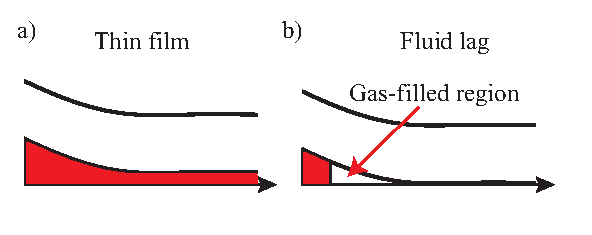
\includegraphics[scale=0.40]{Sketch.eps}
    \caption{Model geometry and parameters. The vertical scale is exaggerated.}
    \label{Figure2-1}
  \end{center}
\end{figure}

As  it  cools,  the  viscosity  of the  fluid  increases  following  a
prescribed rheology $\eta(T)$ given by
\begin{equation}
  \eta(T)=\frac{\eta_h
    \eta_c(T_i-T_0)}{\eta_h(T_i-T_0)+(\eta_c-\eta_h)(T-T_0)}
  \label{rheology}
\end{equation}
where $\eta_h$  and $\eta_c$  are the viscosities  of the  hottest and
coldest  fluid  at  the   temperature  $T_i$  and  $T_0$  respectively
\citep{Bercovici:2007vc}.    Although   this   rheology   is   largely
simplified,  the  inverse  dependence   of  viscosity  on  temperature
captures  the  essential  behavior  of  a  viscous  fluid,  i.e.   the
viscosity  variations are  the largest  where the  temperature is  the
coldest
\citep{Anonymous:CZVBrBvv,Marsh:1981dc,Lejeune:1995fc,Giordano:2008em}.

\subsection{Pressure}
\label{sec:Pressure}

The  intrusion develops  over a  length scale  $\Lambda$ that  is much
larger than its thickness $H$ ($\Lambda >> H$).  In the laminar regime
and  in   axisymmetrical  coordinates  ($r$,$z$),   the  Navier-Stokes
equations under the lubrication assumption are
\begin{eqnarray}
  -\frac{\partial P}{\partial r}  +  \frac{\partial}{\partial z}\left(\eta(T) \frac{\partial u}{\partial z}\right) &=&0\label{V1} \\
  -\frac{\partial P}{\partial z}  - \rho_{m}g&  =&0\label{Npressure}
\end{eqnarray}
where $u(r,z,t)$ is the radial velocity, $\rho_m$ the fluid density, $g$
the standard acceleration  due to gravity and  $P(r,z,t)$ the pressure
within  the fluid.   Integration of  (\ref{Npressure}) gives the
total  pressure  $P(r,z,t)$  within   the  flow.   When  the  vertical
deflection $h(r,t)$  of the upper  elastic layer is small  compared to
its thickness  $d_c$, i.e $h<<d_c$,  we can neglect stretching  of the
upper layer and only consider  bending stresses.  Therefore, the total
pressure $P(r,z,t)$ at a level $z$ in  the current is the sum of three
contributions: the weight of the magma  and of the upper layer and the
bending pressure
\begin{equation}
  P = \rho_m g (h-z)+\rho_rgd_c+D\nabla_r^4h
\end{equation}
where  $h(r,t)$ is  the flow  thickness, $\rho_r$  the density  of the
surrounding rocks and $D$ is the flexural rigidity of the thin elastic
layer, that  depends on Young's  modulus $E$, Poisson's  ratio $\nu^*$
and     on     the     elastic    layer     thickness     $d_c$     as
$D  = Ed_c^3/\left(12(1-\nu^*)\right)$.

\subsection{Injection rate}

Assuming a Poiseuille flow within the cylindrical feeding conduit, the
vertical  injection velocity  $w_i(r,t)$  and injection  rate $Q_0$  are
given by
\begin{equation}
  w_i(r,t)=
  \begin{cases}
    \frac{ \Delta P}{4 \eta_h Z_{c}} (\frac{a^{2}}{4}-r^{2})& r \le \frac{a}{2}\\
    0 & r > \frac{a}{2}
  \end{cases}
  \label{eq12}
\end{equation}
\begin{equation}
  Q_{0}=\frac{\pi \Delta P a^{4}}{128 \eta_h Z_c}
  \label{eq11}
\end{equation}
where  $\Delta P$  is  the  initial overpressure  within  the melt  at
$z=Z_{c}$. 

\subsection{Heat transport equation}
\subsubsection{Local energy conservation}

In the laminar regime and in axisymmetrical coordinates ($r$,$z$), the
local energy  conservation equation within the  lubrication assumption
is written as
\begin{eqnarray}
  \frac{D}{D t}\left(\rho_m C_{p,m} T+\rho_mL(1-\phi)\right)&=& k_m  \frac{\partial^2
                                                                T}{\partial               z^2}\label{EnergyCons}
\end{eqnarray}
where  $T(r,z,t)$ is  the fluid  temperature and  $\rho_m$, $k_m$  and
$C_{p,m}$ are the  density, thermal conductivity and  specific heat of
the fluid.  Here, we also account for energy release by crystallization of
the  fluid, which  is  a non  negligible source  of  heat for  magmas;
$\phi(r,z,t)$ is  the crystal fraction in  the melt and $L$  the latent
heat. In this model, the crystals are considered only as a source/sink
of energy as  they melt/form during flow  emplacement.  In particular,
the physical properties of the fluid  are not modified by the presence
of crystals.

Following a common approximation, we  assume that the crystal fraction
is a linear function of temperature over the melting interval
\begin{equation}
  \phi = \frac{T_L-T}{T_L-T_s}
  \label{meltfraction}
\end{equation}
where $T_S$ and $T_L$ are the solidus and liquidus temperatures of the
magma \citep{Hort:1997hk,Michaut:2006di}. In addition, we assume that
the fluid is  injected as its liquidus temperature ,  i.e. $T_L = T_i$
and, for simplicity, that the solidus  temperature  is  equal  to  the
surrounding rock  temperature $T_S  =T_0$. With  these approximations,
the local energy equation (\ref{EnergyCons}) resumes to
\begin{eqnarray}
  \frac{\partial T}{\partial t}+ u\frac{\partial T}{\partial r}
  + w\frac{\partial T}{\partial z}  &=& \frac{ St}{St+1}\kappa_m  \frac{\partial^2
                                        T}{\partial               z^2}
                                        \label{EnergyCons2}
\end{eqnarray}
where  $u(r,z,t)$ and  $w(r,z,t)$ are  the radial  and vertical  fluid
velocities,  $St  =\left(C_{p,m}(T_i-T_0)\right)/L$   is  the  Stephan
number   and    $\kappa_m$   is   the   fluid    thermal   diffusivity
$\kappa_m = k_m/(\rho_m C_{p,m})$.  We  use an integral balance method
to solve the heat transport equation (\ref{EnergyCons2}).  This theory
is based  on the  integral-balance method  of heat-transfer  theory of
\citet{Goodman:1958ue},  in  which  the   vertical  structure  of  the
temperature field  is represented  by a known  function of  depth that
approximates the expected solution.

\subsubsection{Integral   balance   solution   for   the   temperature
  $T(r,z,t)$}

Following \citet{BALMFORTH:1999ey},  we model the cooling  of the flow
through  the  growth  of  two thermal  boundary  layers:  one  growing
downward from the  top and a second growing upward  from the base.  As
we consider homogeneous thermal  properties for the surrounding rocks,
we assume that the two  thermal boundary layers grow symmetrically and
have  the   same  thickness  $\delta(r,t)$.   We   use  the  following
approximation for the vertical temperature profile $T(r,z,t)$
\begin{equation}
  T=
  \begin{cases}
    T_b - (T_b-T_0)(1-\frac{z}{\delta})^2 & 0 \le z\le \delta \\
    T_b & \delta \le z\le h-\delta \\
    T_b - (T_b-T_0)(1-\frac{h-z}{\delta})^2 & h-\delta \le z\le h\\
  \end{cases}
  \label{Temperature}
\end{equation}
where $T_b(r,t)$  is the temperature at  the center of the  flow.  The
integral balance  solution in  (\ref{Temperature}) assumes  a symmetry
around $z=h/2$  and a decrease of  the temperature in the  two thermal
boundary  layers  down  to  the  surrounding  rock  temperature  $T_0$
\citep{BALMFORTH:1999ey}.    In  addition,   it   assumes  a   uniform
temperature $T_b$  in between the  thermal boundary layers.   As
the fluid is injected at  temperature $T_i$, we have $T_b(r,t) =T_i$
as long as $\delta<h/2$.  However, if the two thermal boundary layers
connect,  then   $\delta  =  h/2$   and  $T_b$  becomes   such  that
$T_b\le T_i$.  This profile assures  the continuity of  the temperature
and heat flux within the flow.


\subsubsection{Integral balance equation}
\label{sec:integr-balance-equat}

We begin by integrating the local energy conservation equation
(\ref{EnergyCons2}) separately  over the two thermal  boundary layers.
The integration  over the  bottom thermal layer,  i.e. from  the base,
$z=0$ to a level $z = \delta$ gives
\begin{eqnarray}
  &&\frac{\partial}{\partial t}\left( \delta( \bar{T}-T_b)\right)+\frac{1}{r}\frac{\partial}{\partial r} \left( r\delta(\overline{uT}-\bar{u}T_b)\right) + \delta\left( \frac{\partial T_b}{\partial t}+ \overline{u}\frac{\partial T_b}{\partial r}\right)\nonumber\\
  &=&-\frac{\kappa_m}{1+St}\left. \frac{\partial T}{\partial z}\right|_{z=0}+w_{i}(T_{i}-T_b)
      \label{Local1}
\end{eqnarray}
where the  bars indicate the  vertical average over the  bottom thermal
boundary layer
\begin{equation}
  \overline{f} = \frac{1}{\delta}\int_0^{\delta}f dz\nonumber,
\end{equation}
$T_b(r,t)$  is  the temperature  at  $z=\delta$,  $w_{i}(r)$ is  the
vertical  injection velocity  and  we  have used  the  nullity of  the
thermal gradient at $z=\delta$ and the local mass conservation
\begin{equation}
  \frac{1}{r}\frac{\partial ru}{\partial r} +\frac{\partial w}{\partial z}=0.
  \label{MassConservation}
\end{equation}
The  integration over  the top  thermal layer,  i.e., from  the level,
$z=h-\delta$ to the top $z=h$ gives
\begin{eqnarray}
  &&\frac{\partial}{\partial t}\left( \delta( \bar{T}-T_b)\right)+\frac{1}{r}\frac{\partial}{\partial r} \left( r\delta(\overline{uT}-\bar{u}T_b)\right) + \delta\left(\frac{\partial T_b}{\partial t}+ \overline{u}\frac{\partial T_b}{\partial r}\right)\nonumber\\
  &=&\frac{\kappa_m}{1+St^{-1}}\left. \frac{\partial T}{\partial z}\right|_{z=h}.
      \label{Local2}
\end{eqnarray}
where,    in    addition    to    the    local    mass    conservation
(\ref{MassConservation})  and the  fact that  the thermal  gradient at
$z=h-\delta$ is  equal to  zero, we have  used the  kinematic boundary
condition in $z=h(r,t)$
\begin{equation}
  \frac{\partial h}{\partial t} +u\frac{\partial h}{\partial
    r} = w
\end{equation}

Therefore,  the  heat  balance   equation,  i.e.   the  heat  equation
(\ref{EnergyCons2})  integrated  over  the  flow  thickness,  is
obtained  by adding  (\ref{Local1})  and (\ref{Local2}).   Introducing
(\ref{Temperature}) to derive the conductive fluxes, we finally obtain
\begin{eqnarray}
  &&\frac{\partial}{\partial t}\left( \delta( \bar{T}-T_b)\right)+\frac{1}{r}\frac{\partial}{\partial r} \left( r\delta(\overline{uT}-\bar{u}T_b)\right) + \delta\left( \frac{\partial T_b}{\partial t}+ \overline{u}\frac{\partial T_b}{\partial r}\right)\nonumber\\
  &=&-\frac{2\kappa_m}{(1+St^{-1})}\frac{\left( T_b - T_0\right)}{\delta}+\frac{w_{i}}{2}(T_{i}-T_b)
      \label{LocalHeat3}
\end{eqnarray}

\subsection{Equation of motion}
\label{sec:equation-motion}

A global statement of mass conservation gives
\begin{eqnarray}
  \frac{\partial h}{\partial t}+ \frac{1}{r}
  \frac{\partial}{\partial
  r} \left( r\int_0^hudz\right)= w_i.
  \label{C3}
\end{eqnarray}
To obtain an  equation for the flow thickness, we  first note that the
chosen vertical structure of the temperature field (\ref{Temperature})
is symmetric  around $h/2$, and  thus, the viscosity and  velocity $u$
possess  the same  symmetry.   Taking advantage  of  this symmetry,  we
integrate              once              (\ref{V1})              using
$\left.\frac{\partial u}{\partial z}\right|_{z=h/2}=0$ to get
\begin{equation}
  \frac{\partial   u}{\partial   z}   =   \frac{1}{\eta}\frac{\partial
    P}{\partial r}\left(z-\frac{h}{2}\right).
  \label{C3-deriv}
\end{equation}
Using no-slip  boundary conditions at  the top  and the bottom  of the
flow,  i.e.  $u(r,z=0,t)=u(r,z=h,t)=0$  equation  (\ref{C3})  can  be
rewritten as
\begin{eqnarray}
  \frac{\partial h}{\partial t} = \frac{1}{r}
  \frac{\partial}{\partial
  r} \left( r\int_0^h\frac{\partial u}{\partial z}zdz\right) + w_i
  \label{C3-Mass}
\end{eqnarray}
and injecting (\ref{C3-deriv}) into  (\ref{C3-Mass}) finally gives the
equation for the flow thickness evolution in axisymmetric coordinates
\begin{eqnarray}
  \frac{\partial h}{\partial t} = \frac{1}{r}
  \frac{\partial}{\partial r} \left( r\left(\rho_m g \frac{\partial h}{\partial      r}+D\frac{\partial}{\partial      r}\left(\nabla_r^4h\right)\right)\left(\int_0^h\frac{1}{\eta(y)}\left(y-\frac{h}{2}\right)ydy\right)\right)
  + w_i.
  \label{C3-Mass-2}
\end{eqnarray}
In  addition,  integration  of   (\ref{C3-deriv})  using  the  no-slip
boundary condition at the base of the flow gives
\begin{equation}
  u(r,z,t) = \frac{\partial P}{\partial r} \int_0^z\frac{1}{\eta(y)}\left(y-\frac{h}{2}\right)dy.
\end{equation}

\subsection{Dimensionless equations}
\label{sec:dimens-equat}

We use the characteristic temperature interval $\Delta T = T_i-T_0$ to
nondimensionalize temperatures.  The dimensionless integral balance
approximation (\ref{Temperature}) becomes
\begin{equation}
  \theta(z)=
  \begin{cases}
    \Theta_b\left(1 -(1-\frac{z}{\delta})^2\right)& 0 \le z\le \delta \\
    \Theta_b & \delta \le z\le h-\delta \\
    \Theta_b\left(1-(1-\frac{h-z}{\delta})^2\right)  &   h-\delta  \le
    z\le h
  \end{cases}
  \label{Temperature2}
\end{equation}
where   $\theta(r,z,t)$   is   the   dimensionless   temperature   and
$\Theta_b=\frac{T_b-T_0}{T_{i}-T_0}$.        Finally,        equations
(\ref{LocalHeat3}) and (\ref{C3-Mass-2})  are nondimensionalized using
a horizontal  scale $\Lambda$, a vertical  scale $H$ and a  time scale
$\tau$ given by
\begin{eqnarray}
  \Lambda &=& \left(\frac{D}{\rho_m g}\right)^{1/4}\label{L1}\\
  H&=&\left       (\frac{12\eta_h      Q_{0}}{\rho_{m}g       \pi}\right      )
       ^{1/4} \label{H1}\\
  \tau&=&\frac{\pi \Lambda^{2} H}{Q_{0}}\label{T1}
\end{eqnarray}
where  $\Lambda$  represents  the  flexural wavelength  of  the  upper
elastic layer \citep{Michaut:2011kg}, $H$ the characteristic thickness
of an isoviscous constant flux gravity current with viscosity $\eta_h$
\citep{Huppert:1982wr} and $\tau$ the characteristic time to fill up a
cylindrical flow of  radius $\Lambda$ and thickness $H$  at a constant
rate $Q_0$.   In addition, we  can define a horizontal  velocity scale
$U=\Lambda/\tau=\left(\rho_m           g           H^3\right)/\left(12
  \eta_h\Lambda\right)$.

The dimensionless equations are
\begin{eqnarray}
  \frac{\partial h}{\partial t}& =& \frac{12}{r}
                                    \frac{\partial}{\partial r} \left( r\left( \frac{\partial h}{\partial      r}+\frac{\partial}{\partial      r}\left(\nabla_r^4h\right)\right)I_1(h)\right)
                                    + w_i\label{EqFinal1}\\
  \frac{\partial}{\partial
  t}\left( \delta( \bar{\theta}-\Theta_b)\right)&=&-\frac{1}{r}\frac{\partial}{\partial
                                                    r}  \left(   r\delta(\overline{u\theta}-\bar{u}\Theta_b)\right)  -
                                                    \delta\left(      \frac{\partial       \Theta_b}{\partial      t}+
                                                    \overline{u}\frac{\partial     \Theta_b}{\partial    r}\right)\nonumber\\
                               &-&
                                   2Pe^{-1}St_m\frac{\Theta_b}{\delta}+\frac{w_{i}}{2}(1-\Theta_b)\label{HeatDimensionLess}\\
  w_{i}&=&
           \frac{32}{\gamma^{2}}\left(\frac{1}{4}-\frac{r^{2}}{\gamma^{2}}\right)\hspace{.2cm}
           \text{if} \hspace{.2cm} r < \gamma/2,\hspace{.2cm} w_i=0 \hspace{.2cm}
           \text{if} \hspace{.2cm} r \ge \gamma/2\\
  u(r,z,t)&   =&   12\left(   \frac{\partial   h}{\partial
                 r}+\frac{\partial}{\partial
                 r}\left(\nabla_r^4h\right)\right)I_0(z)\label{C3-Veloc}
\end{eqnarray}
with
\begin{eqnarray}
  I_0(z)&=&\int_0^z \left(\nu+(1-\nu)\theta(y)\right)\left(y-\frac{h}{2}\right)
            dy \label{I_1}\\
  I_1(z) &=& \int_0^z \left(\nu+(1-\nu)\theta(y)\right)\left(y-\frac{h}{2}\right)y dy\label{I_2}
\end{eqnarray}
and where $\gamma$, $Pe$, $St_m$  and $\nu$ are the four dimensionless
numbers that control the dynamics of the flow
\begin{eqnarray}
  \gamma&=&\frac{a}{\Lambda} \label{gamma}\\
  Pe&=&            \frac{H^2}{\kappa_m            \tau}\label{Pe}\\
  St_m &=& \frac{C_{p,m}\left(T_i-T_0\right)}{C_{p,m}\left(T_i-T_0\right)+L} \label{St}\\
  \nu&=& \frac{\eta_h}{\eta_c}\label{nu}.
\end{eqnarray}
$\gamma$  is the  dimensionless radius  of  the conduit,  it does  not
significantly influence  the flow and is  set to $0.02$ in  this study
\citep{Michaut:2009jx,Michaut:2011kg}; $Pe$ is the Peclet number which
compares the vertical diffusion of heat to the horizontal advection in
the interior; $St_m$ is a modified Stephan number which represents the ratio of
sensible heat between solidus and liquidus  to the total energy of the
fluid  at liquidus  temperature  and $\nu$  is  the maximum  viscosity
contrast, i.e.  the ratio between the hottest and coldest viscosity.

  \subsection{Further simplifications}
  \label{sec:furth-simpl}

  \subsubsection{Heat equation}
  \label{sec:heat-equation}

  The heat balance equations (\ref{HeatDimensionLess}) can reduce to
  \begin{eqnarray}
    \frac{\partial}{\partial
    t}\left( \delta( \bar{\theta}-1)\right)+\frac{1}{r}\frac{\partial}{\partial
    r}
    \left( r\delta(\overline{u\theta}-\bar{u})\right)&=&- 2Pe^{-1}St_m\frac{\Theta_b}{\delta} 
                                                         \label{HeatD_a}
  \end{eqnarray}
  Indeed, if the thermal boundary layers exist, $\Theta_b=1$, $\delta$
  is the  variable and  (\ref{HeatDimensionLess}) directly  reduces to
  (\ref{HeatD_a}).  In contrast, if the thermal boundary layers merge,
  $\delta=h/2$ and the variable is  $\Theta_b$. In this case, the heat
  balance equation (\ref{HeatDimensionLess}) reduces to
  \begin{eqnarray}
    \frac{\partial h\bar{\theta}}{\partial t}+\frac{1}{r}\frac{\partial}{\partial
    r} \left( rh\overline{u\theta}\right)-\Theta_b\left(\frac{\partial h}{\partial t}+\frac{1}{r}\frac{\partial}{\partial
    r} \left( rh\bar{u}\right)\right)&=& - 8St_mPe^{-1}\frac{\Theta_b}{h}+w_{i}(1-\Theta_b)
  \end{eqnarray}
  which, by using (\ref{C3}), rewrites
  \begin{equation}
    \frac{\partial h\bar{\theta}}{\partial t}+\frac{1}{r}\frac{\partial}{\partial
      r} \left( rh\overline{u\theta}\right) &=& w_i
    - 8St_mPe^{-1}\frac{\Theta_b}{h}.
\label{eqHS2}
  \end{equation}
  Equation (\ref{eqHS2}) also corresponds to (\ref{HeatD_a}) when
  $\delta=h/2$.

  Following \citet{BALMFORTH:1999ey}, we rewrite (\ref{HeatD_a}) using
  a new variable $\xi = \delta(1-\overline{\theta})$
  \begin{equation}
    \frac{\partial \xi}{\partial t}+\frac{1}{r}\frac{\partial}{\partial r} \left( r\bar{u}\xi\right)-\frac{1}{r}\frac{\partial}{\partial r} \left( r\delta(\overline{u\theta}-\bar{u}\bar{\theta})\right)&=&2Pe^{-1}St_m\frac{\Theta_b}{\delta}.
    \label{EqFinal2}
  \end{equation}
  where $\Theta_b$  and $\delta$ can  be calculated directly  from the
  expression of $\xi$ such that

\begin{tabular}{p{6cm}p{6cm}}
{
\begin{equation}
    \Theta_b(r)=
    \begin{cases}
      1 &\text{if } \hspace{.5cm} \xi\leq \xi_t \nonumber\\
      \frac{3}{2}-\frac{3\xi}{h} & \text{if} \hspace{.5cm} \xi > \xi_t\nonumber
    \end{cases}
  \end{equation}
                                   }
&
{
  \begin{equation}
    \delta(r)=
    \begin{cases}
      3\xi &\text{if } \hspace{.5cm} \xi\leq \xi_t \nonumber\\
      h(r,t)/2 & \text{if} \hspace{.5cm} \xi > \xi_t\nonumber\\
    \end{cases}
  \end{equation}
  }
\end{tabular}

with $\xi_t = h/6$.

The second term on the left hand side of (\ref{EqFinal2}) contains advection by
the  vertically  integrated  radial  velocity  while  the  third  term
contains a  correction accounting  for the  vertical structure  of the
temperature  field. The  term on  the  right is  the loss  of heat  by
conduction in the surrounding medium.

  \subsubsection{Average quantities}
  The average  velocity over  a thermal boundary  layer $\overline{u}$
  reads
  \begin{eqnarray}
    \overline{u}        =\frac{1}{\delta}\int_0^{\delta}udz        &=&
                                                                       u(r,\delta,t) - \frac{1}{\delta}\int_0^{\delta}\frac{\partial
                                                                       u}{\partial
                                                                       z}
                                                                       zdz\label{eqHello}\\
                                                                   &=&\frac{12}{\delta}
                                                                       \frac{\partial
                                                                       P}{\partial
                                                                       r}\left(\delta
                                                                       I_0(\delta)-I_1(\delta)\right)
  \end{eqnarray}
  where $P(r,z,t) = h+\nabla_r^4h$ is  the dimensionless pressure and we
  have used (\ref{C3-deriv}) in  (\ref{eqHello}).  The average rate of
  heat advected 
  $\overline{u\theta}$ over a thermal boundary layer reads
  \begin{eqnarray}
    \overline{u\theta}=\frac{1}{\delta}\int_0^{\delta}u\theta dz &=& \frac{1}{\delta}\left( [ uG(z) ]_{0}^{\delta} -\int_0^\delta
                                                                     G(z)\frac{\partial
                                                                     u}{\partial
                                                                     z}
                                                                     dz\right)\nonumber\\
                                                                 &=&\frac{12}{\delta} \frac{\partial P}{\partial r}\left(G(\delta)I_0(\delta)-I_2(\delta)\right)
  \end{eqnarray}
  where
  \begin{equation}
    G(z)                  =                 \Theta_b\left(                  z
      +\frac{\delta}{3}\left(1-\frac{z}{\delta}\right)^3\right)
  \end{equation}
  denotes a primitive of $\theta$ when $z<\delta$ and
  \begin{equation}
    I_2(z)=\int_0^y\left(\nu+(1-\nu)\theta(y)\right)G(y)
    \left(y-\frac{h}{2}\right)dy.
    \label{I_3}
  \end{equation}
  Therefore, we have
  \begin{equation}
    \overline{u\theta}-\overline{u}\overline{\theta}= \frac{12}{\delta} \frac{\partial P}{\partial r}\left(I_0(\delta)\left(G(\delta)-\delta\overline{\theta}\right)+\overline{\theta}I_1(\delta)-I_2(\delta)\right)
  \end{equation} 
  where  the average  temperature  over a  thermal  boundary layer  is
  $ \overline{\theta} = 2\Theta_{b}/3$

  \subsection{Summary of the equations}
  \label{sec:summary-equations}

  The  coupled equations  governing the  cooling of  an elastic-plated
  gravity current are summarized in term of the integrals (\ref{I_1}),
  (\ref{I_2}) and (\ref{I_3}) as follow
  \begin{eqnarray}
    \frac{\partial h}{\partial t}-\frac{12}{r}
    \frac{\partial}{\partial      r}
    \left( r I_1(h) \frac{\partial P}{\partial
    r}\right)
    \label{C3-HF}
    & =& \mathcal{H}(\frac{\gamma}{2}-r)\frac{32}{\gamma^{2}}\left(\frac{1}{4}-\frac{r^{2}}{\gamma^{2}}\right)\\
    \frac{\partial                                       \xi}{\partial
    t}+\frac{1}{r}\frac{\partial}{\partial                          r}
    \left( r\left(\bar{u}\xi-\Sigma\right)\right)&=&2Pe^{-1}St_m\frac{\Theta_b}{\delta}\label{C3-TF}
  \end{eqnarray}
  with

\begin{tabular}{p{6cm}p{6cm}}
{
\begin{equation}
    \Theta_b(r)=
    \begin{cases}
      1 &\text{if } \hspace{.5cm} \xi\leq \xi_t \nonumber\\
      \frac{3}{2}-\frac{3\xi}{h} & \text{if} \hspace{.5cm} \xi > \xi_t\nonumber
    \end{cases}
  \end{equation}
                                   }
&
{
  \begin{equation}
    \delta(r)=
    \begin{cases}
      3\xi &\text{if } \hspace{.5cm} \xi\leq \xi_t\\
      h(r,t)/2 & \text{if} \hspace{.5cm} \xi > \xi_t\nonumber\\
    \end{cases}
  \end{equation}
  }
\end{tabular}
\begin{eqnarray}
  \overline{u}&=& \frac{12}{\delta}\frac{\partial P}{\partial r}\left(\delta
                  I_0(\delta)-I_1(\delta)\right) \label{ubarF}\\
  \Sigma     &=& \frac{\partial     P}{\partial
                 r}\left(8I_1(\delta)\Theta_b-12I_2(\delta)\right)\label{SigmaF}
\end{eqnarray}
$P =  h+\nabla_r^4h$ is  the dimensionless pressure  and $\mathcal{H}$
the Heaviside function. The expression of
$I_0(\delta)$, $I_1(h)$,  $I_1(\delta)$ and  $I_2(\delta)$ as  well as
the numerical scheme are given in appendix \ref{Numeric}.

\subsection{Preliminary results for an isothermal flow}
\label{sec:prel-results-isoth}

For a  constant injection  rate, a  small pre-wetting  film thickness,
i.e.   $h_f<<1$ and  a viscosity  contrast $\nu$  set to  1, numerical
resolution  of (\ref{C3-HF})  shows two  asymptotic spreading  regimes
\citep{Michaut:2011kg,Lister:2013ia}.
\begin{figure}
  \begin{center}
    \graphicspath{ {/Users/thorey/Documents/These/Projet/Refroidissement/Skin_Model/Figure/JFM_V13/} }
    \includegraphics[scale=0.45]{Scaling_HR_ELASGRAV_Simple.eps}
    \caption{Left: Dimensionless thickness at  the center $h_0$ versus
      dimensionless  time  $t$.   Dotted-lines: scaling  laws  in  the
      bending  regime $h_0=  0.7h_f^{-1/11}t^{8/22}$  and the  gravity
      regime $h_0$  tends to a constant.   Right: Dimensionless radius
      $R$ versus  dimensionless time $t$.  Dotted-lines:  scaling laws
      in  the bending  regime  $R= 2.2h_f^{1/22}t^{7/22}$  and in  the
      gravity current regime $R\propto t^{1/2}$.}
    \label{Scaling_HR_ELASGRAV_Simple}
  \end{center}
\end{figure}

At  early times,  when  $R<<\Lambda$, gravity  is  negligible and  the
spreading dynamics is governed by the bending of the upper layer.  The
spreading  is  very  slow  and   the  interior  has  uniform  pressure
$P =\nabla_r^4h$.  The flow is  bell-shaped and its thickness is given
by
\begin{equation}
  h(r,t) = h_0(t)\left(1-\frac{r^2}{R^2(t)}\right)^2
  \label{IntrusionShape}
\end{equation}
with   $h_0(t)$  the   thickness  of   the  current   at  the   center
\citep{Michaut:2011kg,Lister:2013ia}.       In       this      regime,
\citet{Lister:2013ia} have  shown that the spreading  is controlled by
the propagation  of a peeling by  bending wave at the  flow front with
dimensionless velocity $c$
\begin{equation}
  c=    \frac{\partial             R}{\partial            t}             =h_f^{1/2}
  \left(\frac{\kappa}{1.35}\right)^{5/2}
  \label{WaveVelocity}
\end{equation}
where  $\kappa  =  \partial^2  h/\partial r^2$  is  the  dimensionless
curvature  of  the  interior  solution.   Using  the  propagation  law
(\ref{WaveVelocity})   and  the   form   of   the  interior   solution
(\ref{IntrusionShape}), they find that the  flow radius and height are
given by the following solutions
\begin{eqnarray}
  h_0(t)&=& 0.7 h_f^{-1/11}t^{8/22}\label{ScalingH}\\
  R(t) &=& 2.2h_f^{1/22}t^{7/22}\label{ScalingR}.
\end{eqnarray}
where the numerical pre-factor obtained in our simulations match those
of \citet{Lister:2013ia} (Figure \ref{Scaling_HR_ELASGRAV_Simple}).

In  contrast,  when  the  radius  R  becomes  larger  than  $4\Lambda$
($R>>\Lambda$), the  weight of the  current becomes dominant  over the
bending  terms.  The  pressure is  given by  the hydrostatic  pressure
$P =  h$ and  the current  enters a  classical gravity  current regime
where bending  terms only  affect the  solution near  the edge  of the
current  \citep{Huppert:1982a,Michaut:2011kg,Lister:2013ia}.  In  this
second regime, the radius evolves as $t^{1/2}$ and the thickness tends
to a constant (Figure \ref{Scaling_HR_ELASGRAV_Simple}).

In  the following,  we study  the effect  of the  cooling on  the flow
dynamics in both regimes separately. We first describe the thermal
structure  for an  isoviscous flow,  i.e. $\nu=1$  and then  study the
effect  of the  temperature-dependent viscosity  on the  flow dynamics
without crystallization, i.e $St_m =1$. Finally, we look at the effect
of crystallization  by setting  $St_m<1$.  For simplicity,  we present
the results for a  given film thickness ($h_f=5\cdot10^{-3}$). Results
for different film thicknesses are shown in Appendix \ref{FilmThickness}.

\section{Numerical approach}
\label{C3-sec:numerical-approach}

\subsection{General procedure}
\label{sec:general-procedure}

The coupled nonlinear partial differential equations (\ref{C3-HF}) and
(\ref{C3-TF}) are solved on a grid of size $M$ defined by the relation
$r_i = (i-0.5)\Delta r$ for $i=1,..,M$. The grid is shifted at the center to avoid
problem arising  from the axisymmetrical  geometry. We index  the grid
point by the indice $i$ and denote the solution on this grid $h_i$ and
$\xi_i$ and the secondary variables $\Theta_{b,i}$, $\Theta_{s,i}$ and
$\delta_i$. Both equations can be expressed on the convenient form
\begin{equation}
  \frac{\partial u}{\partial t} - f = 0
\end{equation}
where $u$  is the function we  want to integrate and  $f$ a non-linear
function  that depends  on $u$.   We  solve these  equations by  first
discretizing all the spatial  derivatives using Finite Difference. The
accuracy of the  scheme is determined by the  higher order derivatives
since  their numerical  approximation requires  the largest  number of
sample points. We then get  two systems of $M$ ordinary differential
equations with the form
\begin{equation}
  \frac{\partial u_i}{\partial t} - f_i = 0 \hspace{1cm} i = 1,...,M
\end{equation}
The time derivatives are first  order and, since explicit schemes tend
to be  very sensitive and unstable,  we use a fully  implicit backward
Euler scheme to get
\begin{equation}
  \frac{u_i^{n+1}-u_i^n}{\Delta t} - f_i(u_i^{n+1}) = 0 \hspace{1cm} i
  = 1,...,M
\label{C3-Num-1}
\end{equation}
Since  $f_i(u_i^{n+1})$ is  not a  linear function,  the system  above
cannot be re-arranged to solve $u_i^{n+1}$ in term of $u_i^{n}$ and an
iterative method  has to  be employed  instead. Fixed  point iteration
method have shown  poor results in converging toward  the solution and
we finally apply  second order Newton's method to  obtain the solution
at each time step.  In particular, we first linearize $u^{n+1}$ around
a guess  of the solution  by assuming $u^{n+1}=u^*+\delta  u^n$, where
$u^*$ is a guess and $\delta u^n$ is the error and we drop the $i$ for
clarity.   Then, we  expressed the  non-linear part  using a  Taylor's
expansion
\begin{equation}
  f^{n+1}=f(u^{n+1})=f(u^*+\delta
  u^n)=f(u^*)+J^h_{f}(u^*)\delta u^n\nonumber
\end{equation}
where  $J^u_{f}(u^*)$ is  the  jacobian matrix  for  the function  $f$
evaluated  in $h^*$.   Injecting the  expansion into  (\ref{C3-Num-1})
finally gives a  system of M linear equations for  the correction term
$\delta_h^n$ which can be expressed as
\begin{equation}
  (I-\Delta tJ^u_{f}(u^*))\delta u^n=u^n-u^*+\Delta t f(u^*)
\end{equation}
where $I$ is the identity matrix. Therefore,  each iteration solves  for $\delta u^n$  and we
use $u_n+\delta u^n$  as a new guess $u^*$ in  each iteration. This is
repeated  until $\delta  u^n$  becomes  sufficiently small.   Finally,
since the equations are coupled, we use a fixed-point iteration method
to  converge  toward  the  solution   $(h,\xi)$  at  each  time  step.
Therefore, the algorithm is the following at each time step
\begin{itemize}
\item Start with a guess for the values of all variables.
\item Solve the thickness equation (\ref{C3-HF}) for $h^{n+1}$ using Newton-Rhapsod method.
\item Solve the heat equation (\ref{C3-TF}) for $\xi^{n+1}$ using $h^{n+1}$ as a new guess for $h^*$
  and Newton-Rhapsod method.
\item Repeat  step one until  further iterations cease to  produce any
  significant changes in the values of both $h^{n+1}$ and $\xi^{n+1}$.
\end{itemize}
The computational scheme is summarized in the following.

\subsection{Thickness equation}

The thickness equation (\ref{C3-HF}) is written as
\begin{eqnarray}
  \frac{\partial h}{\partial t}-f(h,\xi)&=&0
\end{eqnarray}
with
\begin{eqnarray}
  f& =& \frac{1}{r}
        \frac{\partial}{\partial      r}
        \left(      r  \phi\left(     \frac{\partial      }{\partial
        r}\left(h+P\right)\right)\right)+w_i\\
  \phi &=& 12I_1(h)
\end{eqnarray}
and where $P$ is the dimensionless bending pressure $P = \nabla^4h$.

\vspace{.5cm} \textbf{Spatial discretization of f} \vspace{.5cm}

The  spatial discretization  is  obtained using  a central  difference
scheme  over  a  sub-grid  shifted  by $0.5\Delta  r$  from  the  main
grid. Therefore, we have
\begin{eqnarray}
  f_i&=&\frac{1}{r_i \Delta_r}\left(r_{i+1/2}\phi_{i+1/2}\left.\left(\frac{\partial h}{\partial r}+\frac{\partial P}{\partial r}\right)\right|_{i+1/2}-r_{i-1/2}\phi_{i-1/2}\left.\left(\frac{\partial h}{\partial r}+\frac{\partial P}{\partial r}\right)\right|_{i-1/2}\right)\nonumber\\
     &=&A_i\phi_{i+1/2}\left(h_{i+1}-h_i\right)-B_i\phi_{i-1/2}\left(h_{i}-h_{i-1}\right)\nonumber\\
     &+&A_i\phi_{i+1/2}\left(P_{i+1}-P_i\right)-B_i\phi_{i-1/2}\left(P_{i}-P_{i-1}\right)\nonumber\\
     &+&w_i\label{C3-Num-3}
\end{eqnarray}
where                $A_i=r_{i+1/2}/(r_i\Delta_r^2)$               and
$B_i=r_{i-1/2}/(r_i\Delta_r^2)$.   The bending  pressure  term $P$  is
very stiff and  needs a careful treatment.  In  particular, the fourth
order derivative requires a fourth order central difference scheme and
therefore, $P_i$ is  expressed over a seven point stencil  on the main
grid such that
\begin{equation}
  P_{i}=   \alpha_{i}h_{i-3}  +   \beta_{i}h_{i-2}+\gamma_{i}  h_{i-1}
  +\lambda_{i}h_{i}+\kappa_{i}h_{i+1}+\delta_ih_{i+2}+\epsilon_ih_{i+3}
  \label{C3-Num-4}
\end{equation}
with
\begin{eqnarray}
  &\alpha_{i}&=\frac{1}{24\Delta r^{4}}\left(-4+3p_3\Delta_r \right)\nonumber \\
  &\beta_{i}&=\frac{1}{24\Delta r^{4}}\left(48-24p_3\Delta_r-2p_2\Delta_r^2+2p_1\Delta_r^3\right) \nonumber\\
  &\gamma_{i}&=\frac{1}{24\Delta r^{4}}\left(-156+39p_3\Delta_r+32p_2\Delta_r^2-16p_1\Delta_r^3\right)\nonumber\\
  &\lambda_{i}&=\frac{1}{24\Delta r^{4}}\left(224-60p_2\Delta r^{2}\right) \nonumber\\
  &\kappa_{i}&=\frac{1}{24\Delta r^{4}}\left( -156-39p_3\Delta_r+32p_2\Delta_r^2+16p_1\Delta_r^3\right)\nonumber\\
  &\delta_{i}&=\frac{1}{24\Delta r^{4}}\left( 48+24p_3\Delta_r-2p_2\Delta_r^2-2p_1\Delta_r^3\right) \nonumber\\
  &\epsilon_{i}&=\frac{1}{24\Delta r^{4}}\left(-4-3p_3\Delta_r \right)\nonumber
\end{eqnarray}
and where $p_1=1/r_i^3$, $p_2=1/r_i^2$ and $p_3 = 2/r_i$. Finally, the
term $\phi_{i-1/2}$  and $\phi_{i-1/2}$, which depend  on the variable
$\Theta_b$, $\delta$ as well as  different power of $h$, are evaluated
in $i-1/2$ and  $i+1/2$ respectively. Different choices  for the value
of the variable at the mid-cell grid point do not show any significant
difference  and a  simple  average  is taken  such  that the  variable
$u_{i+1/2}$ is taken as $0.5(u_i+u_{i+1})$.

\vspace{.5cm}    \textbf{Expression   of    the   jacobian    $J_f^h$}
\vspace{.5cm}

The discretized  function $f_i$ can be  break down in three  part, the
gravitational part $f_i^{g}$  which is expressed in term  of the value
of $h$ on three  grid points $\left\{{i-1,i,i+1}\right\}$, the bending
part $f_i^{b}$ which is expressed in term  of the value of $h$ on nine
grid points  $\left\{{i-4,i-3,...,i+3,i+4}\right\}$ and  the injection
term which depends only on the grid point $i$ such that
\begin{equation}
  f_i = f_i^g+f_i^b+w_i
\end{equation}
Therefore, the jacobian is  nona-diagonal and its coefficient $J_{il}$
are
\begin{equation}
  J_{il}=
  \begin{cases}
    \frac{\partial f^{b}_i}{\partial h_{l}} &
    l = \left\{{i-4,i-3,i-2,i+2,i+3,i+4}\right\}\\
    \frac{\partial       f^{g}_i}{\partial       h_{l}}+\frac{\partial
      f^{b}_i}{\partial h_{l}} & l =
    \left\{{i-1,i,i+1}\right\}\\
    0 & \text{otherwise}
  \end{cases}
  \label{C2-eq12}
\end{equation}
The different  terms can be  easily derived from  (\ref{C3-Num-3}) and
(\ref{C3-Num-4}) with just slight  adjustment coming from the boundary
conditions.

\vspace{.5cm} \textbf{Boundary condition} \vspace{.5cm}

 We begin with
$h_i=h_f$ for  $i=1,..,M$.  Since the  flow is symmetric in  $r=0$, we
require that
\begin{equation}
  \left.\frac{\partial h}{\partial r}\right|_{r=0} =\left.\frac{\partial P}{\partial r}\right|_{r=0} =0
\end{equation}
and therefore for $i=1$, we have
\begin{eqnarray}
  f_i     &=&A_1\phi_{i+1/2}\left(h_{i+1}-h_i\right)\nonumber\\
          &+&A_i\phi_{i+1/2}\left(P_{i+1}-P_i\right)\nonumber\\
          &+&w_i\label{C3-Num-5}
\end{eqnarray}
The expression  of the  bending pressure, evaluated  over a  $7$ point
stencils, is problematic close to the boundary and reflection formulae
will  be  used  in  order   to  accommodate  the  boundary  conditions
\citet{Patankar:1980vu}.   In   particular,  we  have  $h_0   =  h_1$,
$h_{-1}=h_2$ and  $h_{-2}=h_3$.  Similarly, boundary condition  at the
end of the mesh is accounted by using a grid much larger than the flow
itself and requiring
\begin{equation}
  \left.\frac{\partial h}{\partial r}\right|_{r=r_M} =\left.\frac{\partial P}{\partial r}\right|_{r=r_M} =0
\end{equation}
which gives for $i=M$
\begin{eqnarray}
  f_i     &=&B_i\phi_{i-1/2}\left(h_{i}-h_{i-1}\right)\nonumber\\
          &+&B_i\phi_{i-1/2}\left(P_{i}-P_{i-1}\right)\nonumber\\
          &+&w_i\label{C3-Num-5}
\end{eqnarray}
with $h_{i>=M}=h_f$.


\vspace{.5cm} \textbf{Newton-Rhapsod method} \vspace{.5cm}

The Newton-Rhapsod method reads
\begin{equation}
  (I-\Delta tJ^h_{f}(h_k^*))\delta h_k^n=h^n-h_k^*+\Delta t f(h_k^*)
\end{equation}
where the  $k$ refers  to the $k$  iterations, $I$ is  a $M  \times M$
diagonal  matrix and  $J_f^h(h^*)$  is a  $M  \times M$  nona-diagonal
matrix.  This  system  of  linear  equations can  be  solved  using  a
nona-diagonal algorithm. At the first  iteration, we use $h^*_1 = h^n$
as     a    first     guess    and     then    we     iterate    using
$h^*_k  = h^n+\delta  h_{k-1}^n$ as  a new  guess for  each iterations
until $\delta h^n_{k}$ becomes  sufficiently small.  In particular, we
require that
\begin{equation}
  \delta h^n_k/h^*_{k}<\epsilon
\end{equation}
with $\epsilon = 10^{-4}$. 

\subsection{Heat equation}

The heat equation (\ref{C3-TF}) is written as
\begin{eqnarray}
  \frac{\partial \xi}{\partial t}-g(h,\xi)&=&0
\end{eqnarray}
with
\begin{eqnarray}
  g& =& \frac{1}{r}\frac{\partial}{\partial                          r}
        \left( r\Gamma\xi\right) +\frac{1}{r}\frac{\partial}{\partial                          r}
        \left(r\Sigma\right)+2Pe^{-1}St_m\frac{\left(\Theta_b-\Theta_s\right)}{\delta}\\
  \Gamma&=& -\overline{u}
\end{eqnarray}

\vspace{.5cm} \textbf{Spatial discretization of g} \vspace{.5cm}

As for the thickness equation,  the spatial discretization is obtained
using  a  central  difference  scheme   over  a  sub-grid  shifted  by
$0.5\Delta r$ from the main grid. Therefore, we have
\begin{eqnarray}
  g_i &=& \left(C_i\Gamma_{i+1/2}\xi_{i+1/2}-D_i\Gamma_{i-1/2}\xi_{i-1/2}\right)\\
      &+&\left(C_i\Sigma_{i+1/2}-D_i\Sigma_{i-1/2}\right)\\
      &+&2Pe^{-1}St_m\frac{\Theta_{b,i}-\Theta_{s,i}}{\delta_i}
\end{eqnarray}
with         $C_i         =r_{i+1/2}/(r_i\Delta        r)$         and
$D_i =r_{i-1/2}/(r_i\Delta r)$.   We use the average  between the grid
point $i$ and $i-1$ (resp. $i+1$) to evaluate the quantity in $\Gamma$
and  $\Sigma$ at  $i-1/2$ (resp.   $i+1/2$).   In addition,  we use  a
classical upwind  scheme to handle $\xi$  at the mid grid  point which
requires
\begin{eqnarray}
  \xi_{i+1/2} &=& \xi_i\\
  \xi_{i-1/2} &=& \xi_{i-1}
\end{eqnarray}

\vspace{.5cm}  \textbf{Expression   of  the   Jacobian  $J_{g}^{\xi}$}
\vspace{.5cm}

The expression  of the Jacobian  is much straightforward in  that case
and its coefficient $J_{il}$ are
\begin{equation}
  J_{il}=
  \begin{cases}
    -D_i\Gamma_{i-1/2}&
    l = i-1\\
    C_i\Gamma_{i+1/2} & l = i \\
    0 & \text{otherwise}
  \end{cases}
  \label{C2-eq12}
\end{equation}
with only slight adjustment coming from the boundary conditions.

\vspace{.5cm} \textbf{Boundary conditions} \vspace{.5cm}

We  consider $\Theta_b  =1$  and $\delta  = 10^{-4}$  in  the film  at
$t=0$. In this way, we ensure  that the average temperature across the
film at $t=0$ is close to $1$. By construction, $D_1=0$ and therefore,
for $i=1$ we have
\begin{eqnarray}
  g_i &=& C_i\Gamma_{i+1/2}\xi_{i}+ C_i\Sigma_{i+1/2} +2Pe^{-1}St_m\frac{\Theta_{b,i}-\Theta_{s,i}}{\delta_i}
\end{eqnarray}
For   $i=M$,   we    consider   that   $\Gamma_{i+1/2}=\Gamma_i$   and
$\Sigma_{i=1/2}=\Sigma_i$.   However,  the  choice  for  the  boundary
condition at the border of the grid $i=M$ is not important as we solve
the problem over a grid much larger than the flow itself.

\vspace{.5cm} \textbf{Newton-Rhapsod method} \vspace{.5cm}

The Newton-Rhapsod method reads
\begin{equation}
  (I-\Delta tJ^{\xi}_{g}(\xi_k^*))\delta \xi_k^n=\xi^n-\xi_k^*+\Delta t f(\xi_k^*)
\end{equation}
where the  $k$ refers  to the $k$  iterations, $I$ is  a $M  \times M$
diagonal  matrix and  $J_f^h(\xi^*)$ is  a $M  \times M$  tri-diagonal
matrix.   This  system of  linear  equations  can  be solved  using  a
tri-diagonal algorithm.  As for the  thickness equation, at  the first
iteration,  we use  $\xi^*_1 =  \xi^n$ as  a first  guess and  then we
iterate using $\xi^*_k = \xi^n+\delta  \xi_{k-1}^n$ as a new guess for
each iterations  until $\delta \xi^n_{k}$ becomes  sufficiently small.
In particular, we require that
\begin{equation}
  \delta \xi^n_k/\xi^*_{k}<\epsilon
\end{equation}
with $\epsilon = 10^{-4}$. In addition, at each iteration the quantity
$\Theta^*_{s,k}$, $\Theta^*_{b,k}$ and $\delta^*_k$, that are needed to evaluate $\Gamma$ and
$\Sigma$,  are  derived from  the value of  $\xi^*_{k}$  using
(\ref{C3-TS}), (\ref{C3-TB}) and (\ref{C3-DELTA}) respectively.

\section{Evolution in the bending regime}
\label{sec:evol-bend-regime}

We first concentrate on the case  in which only bending contributes to
the dynamics pressure.  The governing equations are thus (\ref{C3-HF}) and
(\ref{C3-TF}) where  $P=\nabla_r^4h$.  

\subsection{Thermal structure for an isoviscous flow, effect of $Pe$}
\label{sec:thermal-structure-an}

The current  cools by conduction  and thermal boundary layers  form at
the contact with the surrounding  medium.  These boundary layers first
connect at the  tip of the flow, where the  small thickness induces an
important  cooling (Figure  \ref{Grid_Time_ELAS}).  A  region of  cold
fluid forms at the front.

As the  current thickens  with time, a  balance between  advection and
diffusion of heat is never reached in the interior of the current. The
hot thermal  anomaly grows in extent  with time but it  extends slower
than the  current itself and  the cold fluid  region at the  tip grows
even faster.   For instance, for $Pe  =100$, while the region  of cold
fluid extends over about $10\%$ of  the current at $t=0.5$, it extends
over  about  $20\%$ at  $t  =10$  (Figure \ref{Grid_Time_ELAS}).   The
smaller $Pe$,  the more  important the  conductive
cooling   and  the   larger   the  cold   fluid   region  is   (Figure
\ref{Thickness_Temperature_Profile_ELAS}   and  \ref{Grid_PeNu_ELAS}).
For  instance, at  $t=10$, while  the cold  fluid region  extends over
about $20\%$  of the current for  $Pe=100$, it extends over  more than
$70\%$ for $Pe=1$ (Figure \ref{Grid_PeNu_ELAS}).

\begin{figure}
  \begin{center}
    \graphicspath{ {/Users/thorey/Documents/These/Projet/Refroidissement/Skin_Model/Figure/JFM_V13/} }
    \includegraphics[scale=0.35]{Grid_Time_ELAS_Pe1_Nu1.eps}
    \caption{Snapshots of  the flow thermal  structure $\theta(r,z,t)$
      at  different  times  indicated   on  the  plot.   Dashed  lines
      represent  the thermal  boundary  layers. Solid  grey lines  are
      isotherms for  $\theta =  0.2$, $0.4$,  $0.6$ and  $0.8$.  Here,
      $\nu=1$, $Pe =100$, $St_m = 1$.}
    \label{Grid_Time_ELAS}
  \end{center}
\end{figure}

\begin{figure}
  \begin{center}
    \graphicspath{ {/Users/thorey/Documents/These/Projet/Refroidissement/Skin_Model/Figure/JFM_V13/} }
    \includegraphics[scale=0.4]{Thickness_Temperature_Profile_ELAS.eps}
    \caption{Left: thickness normalized by the thickness at the center
      $h(r,t)/h_0(t)$  versus radial  axis normalized  by the  current
      radius $r/R(t)$  at different  times indicated  on the  plot for
      $Pe=1$   and  $\nu=1.0$.    Solid-lines  represent   the
      thickness profiles.   Dashed-lines represent the thermal
      boundary layers.  Right: Same plot but for $\nu=10^{-3}$.}
    \label{Thickness_Temperature_Profile_ELAS}
  \end{center}
\end{figure}

\begin{figure}
  \begin{center}
    \graphicspath{ {/Users/thorey/Documents/These/Projet/Refroidissement/Skin_Model/Figure/JFM_V13/} }
    \includegraphics[scale=0.48]{Grid_PeNu_ELAS_Final_2.eps}
    \caption{Snapshots of  the flow thermal  structure $\theta(r,z,t)$
      for different set ($\nu$,$Pe$) with  $\nu= 1$, $0.1$, $0.01$ and
      $0.001$  and $Pe=1$,  $10$, $100$  and $1000$  at $t=10$.  While
      $Pe$ controls the  thermal structure of the flow, it  has only a
      small influence on the flow aspect ratio which is controlled by $\nu$.}
    \label{Grid_PeNu_ELAS}
  \end{center}
\end{figure}

\subsection{Thickness and temperature profile, effect of $\nu$}
\label{sec:thickn-temp-prof-1-e}

When accounting for  the temperature dependence of  the viscosity, the
region of cold  fluid at the tip  is marked by a  higher viscosity and
enhances flow thickening at the  expense of spreading.  The larger the
viscosity  contrast,  the  larger  the aspect  ratio  $h_0/R$  (Figure
\ref{Grid_PeNu_ELAS}).  For  instance, for  the same value  of $Pe=1$,
while the aspect ratio is $0.7$ for $\nu=1$ at $t=10$, it is $4.2$ for
the  same   time  and  $\nu=10^{-3}$   (Figure  \ref{Grid_PeNu_ELAS}).
Nevertheless, the  shape of the flow  remains essentially self-similar
(\ref{IntrusionShape}) and cannot be  differentiated from the shape of
an isoviscous current  if the thickness and the  radial coordinates are
rescaled by  the thickness  at the center  $h_0(t)$ and  radius $R(t)$
(Figure \ref{Thickness_Temperature_Profile_ELAS}).

The flow thermal  structure is similar to the  isoviscous case (Figure
\ref{Grid_PeNu_ELAS}), the  thermal anomaly rapidly detaches  from the
tip of the  current and a region  of cold fluid develops  at the front
where  the heat  loss is  largest. However,  the important  thickening
induced by the viscosity increase limits heat loss to the surrounding.
The  larger  the viscosity  contrast  $\nu$,  the more  important  the
thickening and  the larger the thermal  anomaly at a given  time.  For
instance, for  $Pe=1$, while  the thermal  anomaly extends  over about
$30\%$ of  the flow for $\nu=1$  at $t=10$, it extends  over more than
$50\%$ for $\nu=10^{-3}$ (Figure \ref{Grid_PeNu_ELAS}).

As expected, a larger Peclet number  leads to a larger thermal anomaly
(Figure  \ref{Grid_PeNu_ELAS}).   However, although  different  Peclet
numbers cause very  different thermal structures, the  influence of the
Peclet number on  the flow morphology is small, much  smaller than the
effect of the viscosity contrast $\nu$ (Figure \ref{Grid_PeNu_ELAS}).  For instance, for
$\nu=10^{-3}$ at $t=10$, the thermal  anomaly is still attached to the
tip of the current for $Pe = 1000$ whereas it makes about $50\%$ of the
current for $Pe=1$; but, the thickness $h_0$ and the
radius $R$ in both cases differ only by a few percents (Figure
\ref{Grid_PeNu_ELAS}). This suggests that the
spreading of  the flow is  not controlled  by the mean  temperature or
average viscosity of the flow. 
  
\subsection{Evolution of the thickness and the radius}
\label{sec:evol-thickn-radi-e}

The dynamics show three different  spreading phases.  The thickness as
well as the radius first follow  the isoviscous scaling laws for a hot
viscosity   current   $h_0\propto   t^{8/22}$   (\ref{ScalingH})   and
$R\propto  t^{7/22}$ (\ref{ScalingR})  (Figure \ref{Scaling_HR_ELAS}).
In the  second phase,  thickening occurs at  the expense  of spreading
because the thermal  anomaly has detached from the  current radius and
the viscous cold fluid region at the front slows down the spreading.
Finally, the  dynamics enters  a third phase  where the  thickness and
radius  follow the  scaling laws  for the  spreading of  an isoviscous
current characterized by a dimensionless cold viscosity $1/\nu$. These
scaling laws  are obtained from (\ref{ScalingH})  and (\ref{ScalingR})
by rescaling the characteristic thickness and time by $\nu^{1/4}$ and
read
\begin{eqnarray}
  h_{0} & = &0.7 \nu^{-2/11} h_f^{-2/22}t^{8/22}\label{ScalingH-Visco}\\
  R& = & 2.2 \nu^{1/11}h_f^{1/22} t^{7/22}\label{ScalingR-Visco}.
\end{eqnarray}
\begin{figure}
  \begin{center}
    \graphicspath{ {/Users/thorey/Documents/These/Projet/Refroidissement/Skin_Model/Figure/JFM_V13/} }
    \includegraphics[scale=0.45]{Scaling_HR_ELAS.eps}
    \caption{Left: Dimensionless thickness at  the center $h_0$ versus
      dimensionless time  $t$ for different sets  $(\nu,Pe)$ indicated
      on      the      plot.      Dotted-lines:      scaling      laws
      $h_0=  0.7h_f^{-1/11}\nu^{-2/11}t^{8/22}$ for  $\nu  = 1.0$  and
      $0.001$.  Right:  Dimensionless radius $R$  versus dimensionless
      time  $t$  for  the  same sets  $(\nu,Pe)$.   Dotted-lines:  the
      scaling    laws    $R=   2.2h_f^{1/22}\nu^{1/11}t^{7/22}$    for
      $\nu = 1.0$ and $0.001$.}
    \label{Scaling_HR_ELAS}
  \end{center}
\end{figure}
The dependence on  the viscosity contrast $\nu$ indeed  fits very well
the  third phase  of the  flow observed  in the  numerical simulations
(Figure  \ref{Scaling_HR_ELAS}).   These   results  suggest  that  the
effective viscosity $\eta_e$  that governs the flow  dynamics is first
close to the  viscosity of the hot fluid; it  rapidly increases in the
second phase  to asymptotically tend to  the one of the  cold fluid in
the third phase.

The time  the flow spends in  each phase depends on  the Peclet number
$Pe$.  For instance,  for $\nu=10^{-3}$, while the  current leaves the
first phase at $t \sim 10^{-6}$ for $Pe =1.0$, this transition happens
only   after   $t   \sim   10^{-2}$    for   $Pe   =   10^3$   (Figure
\ref{Scaling_HR_ELAS}).  The  larger  the   Peclet  number,  the  less
efficient the  cooling, and thus  the longer  the flow remains  in the
first  phase  and the  later  it  reaches  the  third phase.

\subsection{Characterization of the thermal anomaly}
\label{sec:char-therm-anom-e}

Following \citet{Garel:2012bh},  we quantify  the size of  the thermal
anomaly  through   a  critical  thermal  radius   $R_c(t)$  where  the
temperature  at the  center of  the flow  $\Theta_b$ is  $1\%$ of  the
injection temperature, i.e. $\Theta_b(r=0)-\Theta_b(r=R_c) = 0.99$.

The thermal  anomaly is first advected  at the same velocity as the
current itself,  i.e.  $R(t) = R_c(t)$  (Figure \ref{R_Rc_ELAS} left).
After  a time  that depends  on $Pe$  and $\nu$,  the thermal  anomaly
detaches from  the tip and  $R(t)-R_c(t)$ increases with  time (Figure
\ref{R_Rc_ELAS}) .

In  the bending  regime, the  interior  pressure is  constant and  the
thickness profile  $h(r)$ is  given by  (\ref{IntrusionShape}) (Figure
\ref{Thickness_Temperature_Profile_ELAS}).   The size  of the  thermal
anomaly $R_c(t)$  is given by  the radius  where advection of  heat is
equal to heat loss
\begin{equation}
  \frac{d}{d    t}\left(\theta(r=   R_c,t)\right)    \propto   Pe^{-1}
  \frac{\partial^2}{\partial z^2}\left(\theta(r=R_c,t)\right).
  \label{HeatequationThermal}
\end{equation}
Assuming  that,  at the  edge  of  the  thermal anomaly,  $\theta$  is
constant and  close to  $\Theta_b$, i.e. $\theta\approx  \Theta_b$, we
obtain by  integrating (\ref{HeatequationThermal}) over $h$  and using
(\ref{Temperature2})
\begin{eqnarray}
  \frac{d}{dt}\left(\int_0^h\theta dz\right)&\propto& Pe^{-1} \frac{\Theta_b}{h}\nonumber\\
  \Theta_b\frac{d  h}{d   t}&\propto& Pe^{-1}
                                      \frac{\Theta_b}{h}\nonumber\\
  \frac{d h}{d t}&\propto& \frac{Pe^{-1}}{h}\label{Calcul1}.
\end{eqnarray}
Using  the thickness  profile (\ref{IntrusionShape}),  (\ref{Calcul1})
becomes
\begin{eqnarray}
  \alpha^2\left(1+\frac{R_c}{R}\right)^2\frac{\partial h_0}{\partial
  t}+\frac{4h_0R_c^2}{R^3}\frac{\partial
  R}{\partial
  t}\alpha\left(1+\frac{R_c}{R}\right) =\frac{Pe^{-1}}{\alpha^2\left(1+\frac{R_c}{R}\right)^2h_0}\nonumber
\end{eqnarray}
where we  introduce $\alpha (t)=  \left(R(t)-R_c(t)\right)/R(t)$, i.e.
the normalized  region beyond  $r=R_c(t)$.  In the  limit $\alpha<<1$,
i.e. $R_c/R\sim 1$ and discarding higher-order terms, we finally get
\begin{equation}
  \alpha^3\propto \frac{Pe^{-1}} {h_0^2(t)}\frac{R}{\frac{\partial R}{\partial t}}.
\end{equation}
Substituting  the  thickness  $h_0(t)$  and the  radius
$R(t)$ by  their respective scaling laws  (\ref{ScalingH-Visco}) and
(\ref{ScalingR-Visco}), the relative size of the normalized cold front
region $\alpha$ reads
\begin{equation}
  \alpha(t)&\propto& Pe^{-1/3}\nu^{4/33} h_f^{2/33}t^{1/11}.
  \label{ScalingXi}
\end{equation}
which is equivalent to
\begin{equation}
  R(t)-R_c(t) = 2.1 Pe^{-1/3}\nu^{7/33} h_f^{7/66}t^{9/22}
  \label{ScalingRRc}
\end{equation}
where the  numerically prefactor, which  depends on the  definition of
the thermal anomaly, has been chosen to fit the simulations.
\begin{figure}
  \begin{center}
    \graphicspath{ {/Users/thorey/Documents/These/Projet/Refroidissement/Skin_Model/Figure/JFM_V13/} }
    \includegraphics[scale=0.45]{R_Rc_ELAS.eps}
    \caption{Left:  Extent  of  the cold  fluid  region  $R(t)-R_c(t)$
      versus   dimensionless    time   for    different   combinations
      ($\nu$,$Pe$) indicated on the plot.   Right: Same plot but where
      we   rescale  the   extent   of  the   cold   fluid  region   by
      $Pe^{-1/3}\nu^{7/33}$.       Dotted-line:       scaling      law
      $(R(t)-R_c(t))Pe^{1/3}\nu^{-7/33}= 2.1 h_f^{7/66}t^{9/22}$.}
    \label{R_Rc_ELAS}
  \end{center}
\end{figure}

The predicted  scaling law  for the  extent of  the cold  fluid region
(\ref{ScalingRRc}) indeed  closely fits the numerical  simulations for
$\nu<1$ and the different Peclet numbers (Figure \ref{R_Rc_ELAS}). For
$\nu=1$ and $Pe=1$, the condition  $R-R_c<<R$ is no more respected for
$t>0.1$, the thermal anomaly is much  smaller than the flow itself and
the scaling law (\ref{ScalingRRc}) is no more applicable as expected.

\subsection{Effective viscosity of the current}
\label{sec:effect-visc-blist-e}

We  use  the   predicted  scaling  law  for   the  thickness  $h_0(t)$
(\ref{ScalingH-Visco}) to  infer the  time evolution of  the effective
viscosity    $\eta_e(t)$.      Indeed,    substituting     $\nu$    by
$\eta_h/\eta_e(t)$   in  (\ref{ScalingH-Visco})   and  inverting   for
$\eta_e(t)/\eta_h$, we get
\begin{eqnarray}
  \eta_e(t)/\eta_h&=& \left(\frac{h_0(t)t^{-8/22}}{0.7 h_f^{-2/22}}\right)^{11/2}\label{eff-visco}
\end{eqnarray}
where $h_0(t)$ is given by the simulation.
\begin{figure}
  \begin{center}
    \graphicspath{ {/Users/thorey/Documents/These/Projet/Refroidissement/Skin_Model/Figure/JFM_V13/} }
    \includegraphics[scale=0.45]{Visco_ELAS_Version_2.eps}
    \caption{Top:  Dimensionless   viscosity  $\eta(t)/\eta_h$  versus
      dimensionless time  t for  different combinations  ($\nu$, $Pe$)
      indicated  on  the  plot.    Solid  lines:  effective  viscosity
      $\eta_e/\eta_h$  defined  by  (\ref{eff-visco}).   Dashed-lines:
      average         flow         viscosity        defined         by
      $\overline{\eta_a(t)}/\eta_h                                   =
      \frac{1}{V(t)}\int_0^{R(t)}\int_0^{h(r,t)} r \eta(\theta) dr dz$
      where $V(t)$ is the current volume.  Dotted-lines: average front
      viscosity   $\eta_f/\eta_h$   defined  by   (\ref{front-visco}).
      Bottom left:  dimensionless effective viscosity  $\eta_e$ versus
      time where the  time has been rescaled by the  time for the flow
      to enter the second phase  $t_{b2}$.  Bottom right: Same as left
      but where the time has been rescaled by the time for the flow to
      enter the third phase $t_{b3}$.  }
    \label{Visco_ELAS_Version_2}
  \end{center}
\end{figure}

As suggested  by the results of  section \ref{sec:evol-thickn-radi-e},
the effective viscosity is first  close to the hot viscosity $\eta_h$,
i.e.   $\eta_e/\eta_h \sim  1$.  It  rapidly increases  in the  second
phase of propagation and finally  tends to the cold viscosity $\eta_c$
in  the   third  phase,  i.e.   $\eta_e/\eta_h   \sim  1/\nu$  (Figure
\ref{Visco_ELAS_Version_2} top).  The spreading in the isoviscous case
is controlled by  the propagation of a peeling by  bending wave at the
tip of the current  \citep{Lister:2013ia}.  In agreement, the behavior
of the effective viscosity has to  be linked with the rapid cooling of
the  front.   To  test  this  hypothesis,  we  calculate  the  average
viscosity $\eta_f(t)$ over a fixed front region of size $L$ in between
$R(t)-L$ and $R(t)$ such that
\begin{eqnarray}
  \eta_f/\eta_h =
  \frac{1}{V_f}\int_{R-L}^{R}\int_0^{h}  r  \eta(\theta)
  dr dz \label{front-visco}
\end{eqnarray}
where $V_f(t)$ is the volume of this region.  The numerical evaluation
of $\eta_f(t)$ for a constant size $L \sim 0.1$ gives a good agreement
with the evolution of the  effective viscosity $\eta_e$ for the second
phase of propagation  (Figure \ref{Visco_ELAS_Version_2}).  Therefore,
the effective viscosity, and thus the different phases of propagation,
are controlled by the average viscosity of a small region at the front
of the current.

At the  initiation of  the flow,  the pre-wetted  film is  composed by
fluid at the injection temperature, the thermal anomaly is attached to
the front  and the current spreads  with a hot viscosity  $\eta_h$. As
soon as the film has cooled, the thermal anomaly detaches from the tip
of  the  current and  the  effective  viscosity increases.   The  time
$t_{b2}$ the current enters this second  phase of the flow thus scales
as the time to cool the  pre-wetted film thickness by conduction, i.e.
$t_{b2}=0.1Peh_f^2$ where the numerical  prefactor has been matched to
the simulations.  Indeed, when rescaling the time of the simulations by
$t_{b2}$, the different combinations $(\nu,Pe)$ enter the second phase
simultaneously   (Figure  \ref{Visco_ELAS_Version_2},   bottom  left).
Then, the  size of the cold  fluid region at the  front increases, the
effective viscosity  increases, and when $R(t)-R_c(t)$  becomes larger
than $\sim  0.1$, the  current behaves as  an isoviscous  current with
cold viscosity $\eta_c$.  Therefore, the time $t_{b3}$ for the flow to
enter this third  phase scales as the time for  the cold fluid region,
whose  size  is  given  by   (\ref{ScalingRRc}),  to  be  larger  than
$\sim 0.1$. In  particular, we define the time $t_{b3}$  as the time for
the  effective  to  reach  $90\%$   of  its  maximum  value  $\eta_c$.
Inverting (\ref{ScalingRRc})  and matching the numerical  prefactor to
the                simulation                thus                gives
$t_{b3}\sim  0.01  Pe^{22/27}\nu^{-14/27}h_f^{-7/27}$.   Indeed,  when
rescaling  the time  of  the simulations  by  $t_{b3}$, the  different
combinations $(\nu,Pe)$  enter the third phase  simultaneously (Figure
\ref{Visco_ELAS_Version_2}, bottom right).

\subsection{Note on the effect of crystallization}
\label{sec:note-effect-cryst-1}

Here, we  examine the effect  of crystallization on the  flow dynamics
and use  values of $St_m <  1$.  Crystallization induces a  release of
latent heat in the fluid, increasing the amount of available energy at
a given time.
\begin{figure}
  \begin{center}
    \graphicspath{ {/Users/thorey/Documents/These/Projet/Refroidissement/Skin_Model/Figure/JFM_V13/} }
    \includegraphics[scale=0.45]{Scaling_HR_ELAS_Stm.eps}
    \caption{Left: Dimensionless thickness at  the center $h_0$ versus
      dimensionless time $t$ for  different values of $St_m$ indicated
      on the  plot, $\nu=0.001$ and $Pe  =10.0$.  Dotted-line: scaling
      law $h_0= 0.7h_f^{-1/11}\nu^{-2/11}t^{8/22}$  for $\nu = 0.001$.
      Right: Dimensionless  radius $R$  versus dimensionless  time $t$
      for  the same  combinations  of  dimensionless numbers.   Dotted
      lines:  scaling  law $R=  2.2h_f^{1/22}\nu^{1/11}t^{7/22}$  for
      $\nu = 0.001$.}
    \label{Scaling_HR_ELAS_Stm}
  \end{center}
\end{figure}
When $St_m<1$,  the tip of the  current remains hot for  a longer time
and the  flow transitions to the  second phase later than  in the case
where   $St_m=1$    (Figure   \ref{Scaling_HR_ELAS_Stm}).     As   the
crystallization  acts only  to reduce  the  cooling term  by a  factor
$St_m$ in (\ref{C3-TF}), one  can easily rewrite (\ref{ScalingRRc}) to
acount for the effect of crystallization on the size of the cold fluid
region
\begin{equation}
  R(t)-R_c(t) =2.1Pe^{-1/3}St_m^{1/3}\nu^{7/33}
  h_f^{7/66}t^{9/22}.\label{ScalingRRcFinal}\\
\end{equation}
Indeed, the  dependence with the  dimensionless number $St_m$  is well
described   by  the   scaling   law  (\ref{ScalingRRcFinal})   (Figure
\ref{R_Rc_ELAS_Stm}).  Accordingly, the time $t_{b2}$ and $t_{b3}$ for
the  current  to  enter  the  second  and  third  phase  of  the  flow
respectively are delayed and when accounting for crystallization read
\begin{eqnarray}
  t_{b2}&\sim&0.1Pe St_m^{-1} h_f^2\label{tb2}\\
  t_{b3}&\sim&   10^{-2}  St_m^{-22/27}Pe^{22/27}\nu^{-14/27}h_f^{-7/27}\label{tb3}
\end{eqnarray}
\begin{figure}
  \begin{center}
    \graphicspath{ {/Users/thorey/Documents/These/Projet/Refroidissement/Skin_Model/Figure/JFM_V13/} }
    \includegraphics[scale=0.45]{R_Rc_ELAS_Stm.eps}
    \caption{Left:  Extent  of  the cold  fluid  region  $R(t)-R_c(t)$
      versus   dimensionless    time   for    different   combinations
      ($\nu$,$St_m$) indicated  on the  plot and $Pe=1$.   Right: Same
      plot but  where we have  rescaled the  extent of the  cold fluid
      region  by  $St_m^{1/3}\nu^{7/33}$.   Dotted-line:  scaling  law
      $(R(t)-R_c(t))St_m^{-1/3}\nu^{-7/33}=                  2.1
      h_f^{7/66}t^{9/22}$.}
    \label{R_Rc_ELAS_Stm}
  \end{center}
\end{figure}


\section{Evolution in the gravity current regime}
\label{sec:evol-grav-curr-1}

To study the late time behavior, we concentrate on the case where only
the weight  of the fluid  contributes to the pressure.   The governing
equation  are thus  (\ref{C3-HF}) and  (\ref{C3-TF}) where  $P=h$.  We
follow      the     same      development  as      in     Section
\ref{sec:evol-bend-regime}.   In  particular,  we first  describe  the
thermal structure for an isoviscous flow, i.e. $\nu=1$, then we study
the effect of the temperature-dependent viscosity on the current
dynamics without crystallization, i.e.  $\nu<1$ and $St_m=1$. Finally,
we look at the effect of crystallization by setting $St_m<1$.

\subsection{Thermal structure for an isoviscous flow, effect of $Pe$}
\label{sec:thermal-structure-an-1}
  
As in the bending  regime, the bulk of the fluid  first expands at the
injection temperature and $R_c \sim R$.  As the bottom and the top cool
by conduction,  thermal boundary layers  form at the contact  with the
surrounding medium and connect at the  tip of the current. However, in
the gravity  current regime, the thickness  of the current tends  to a
constant.   Therefore, conduction  in the  surrounding medium  rapidly
balances the input of heat at  the center and when the thermal anomaly
detaches from the tip of the current, its extent reaches a steady state
profile (Figure \ref{Grid_Time_GRAV}).

\begin{figure}
  \begin{center}
    \graphicspath{ {/Users/thorey/Documents/These/Projet/Refroidissement/Skin_Model/Figure/JFM_V13/} }
    \includegraphics[scale=0.35]{Grid_Time_GRAV_Pe1_Nu1.eps}
    \caption{Snapshots of  the flow thermal  structure $\theta(r,z,t)$
      at different times indicated on the plot.  Dashed lines: thermal
      boundary layers.  Here, $\nu=1$, $Pe =100$ and $St_m = 1$.}
    \label{Grid_Time_GRAV}
  \end{center}
\end{figure}

The radius of the steady state  thermal anomaly $R_c$ depends on $Pe$.
In  particular, the  larger the  number  $Pe$, the  larger the  radius
$R_c$ is. For instance, for $\nu=1$, while the thermal anomaly $R_c$ is less than $1$
in the  steady state  regime for  $Pe=1$, it  is about
$12$ for $Pe=10^3$ (Figure \ref{Grid_PeNu_GRAV}).

\begin{figure}
  \begin{center}
    \graphicspath{ {/Users/thorey/Documents/These/Projet/Refroidissement/Skin_Model/Figure/JFM_V13/} }
    \includegraphics[scale=0.45]{Grid_PeNu_GRAV_Final_2.eps}
    \caption{Snapshots of  the flow thermal  structure $\theta(r,z,t)$
      for different sets ($\nu$,$Pe$) with $\nu= 1$ ,$0.1$ ,$0.01$ and
      $0.001$ and  $Pe=1$, $10$,  $100$ and  $1000$ at  $t=200$.}
    \label{Grid_PeNu_GRAV}
  \end{center}
\end{figure}

\subsection{Thickness and temperature profile, effect of $\nu$}
\label{sec:thickn-temp-prof}

For a current with a viscosity that depends on temperature, as soon as
the thermal anomaly  detaches from the current radius,  the cold fluid
at  the  front tends  to  slow  down  the  spreading and  enhance  the
thickening of  the flow (Figure \ref{Grid_PeNu_GRAV}).   For instance,
for $Pe=1$, while the aspect ratio $h_0/R$ is about $0.12$ for $\nu=1$
at   $t=200$,    it   is   $\sim   1$    for   $\nu=10^{-3}$   (Figure
\ref{Grid_PeNu_GRAV}).  The  shape of the current  is not self-similar
and the front  steepens when the viscosity increases  in comparison to
the isoviscous case as  in \citet{Bercovici:2007vc}. However, when the
current becomes much larger than the thermal anomaly, the current side
slumps to become less steep (Figure \ref{Grid_PeNu_GRAV}) and recovers
a shape similar to the isoviscous flow with cold viscosity.

The  thermal  structure  is  similar   to  the  isoviscous  case.   In
particular, after  a time  that depends on  $Pe$, the  thermal anomaly
reaches a  steady-state profile (Figure \ref{Grid_PeNu_GRAV}).   As in
the bending regime,  the thickening at the center limits  heat loss to
the  surrounding for  large values  of the  viscosity contrast  $\nu$.
Therefore, the  extent of the  thermal anomaly in the  steady-state is
slightly larger  for a larger  viscosity contrast.  For  instance, for
$Pe=10$ at $t=200$,  while the thermal anomaly extends  over less than
$2$ for $\nu=1$, it reaches $Rc\sim3$ for $\nu=10^{-3}$.

The  flow morphology  is  more sensitive  to the  $Pe$  number in  the
gravity current regime  than in the bending regime  and different $Pe$
lead  to different  current  morphologies for  a  given $\nu$  (Figure
\ref{Grid_PeNu_GRAV}).   For instance,  for $\nu=10^{-3}$  at $t=200$,
the thermal  anomaly is still attached  to the tip of  the current for
$Pe =  10^3$ and  the aspect  ratio of  the flow  $h_0/R$ is  close to
$0.15$.  In contrast, for $Pe=1$,  the thermal anomaly radius $R_c$ is
less than  $30\%$ of the  current radius and  the aspect ratio  of the
flow is much larger $h_0/R = 1.15$ (Figure \ref{Grid_PeNu_GRAV}).

\subsection{Evolution of the thickness and the radius}
\label{sec:evol-thickn-radi-g}
  
As in the bending regime,  the dynamics show three different spreading
phases.   The  thickness  as  well  as the  radius  first  follow  the
isoviscous  scaling laws  for  a given  hot  viscosity $\eta_h$,  i.e.
$h_0$   tends   to  a   constant   and   $R\propto  t^{1/2}$   (Figure
\ref{Scaling_HR_GRAV}).   In a  second  phase,  the thickness  rapidly
increases and  the spreading slows  down.  Finally, the  thickness and
radius follow  the isoviscous  scaling laws but  for a  cold viscosity
flow.

These dimensionless scaling laws read, as a function of $\nu$
\begin{figure}
  \begin{center}
    \graphicspath{ {/Users/thorey/Documents/These/Projet/Refroidissement/Skin_Model/Figure/JFM_V13/} }
    \includegraphics[scale=0.45]{Scaling_HR_GRAV.eps}
    \caption{Left: Dimensionless thickness at  the center $h_0$ versus
      dimensionless time  $t$ for different sets  $(\nu,Pe)$ indicated
      on   the  plot.    Dotted-lines  represent   the  scaling   laws
      $h_0=  2.1\nu^{-1/4}$ for  $\nu  = 1.0$  and $10^{-2}$.   Right:
      Dimensionless radius  $R$ versus dimensionless time  $t$ for the
      same sets  $(\nu,Pe)$.  Dotted-lines represent the  scaling laws
      $R= 1.1\nu^{1/8}t^{1/2}$ for $\nu = 1.0$ and $10^{-2}$.}
    \label{Scaling_HR_GRAV}
  \end{center}
\end{figure}
\begin{eqnarray}
  h_0 &=& 2.1\nu^{-1/4}\label{scaling-H-gravi-2}\\
  R(t) &=& 1.1\nu^{1/8} t^{1/2}\label{scaling-R-gravi-2}
\end{eqnarray}
They   perfectly    matched   our   numerical    simulations   (Figure
\ref{Scaling_HR_GRAV}).  Therefore,  the effective  viscosity $\eta_e$
that controls the flow dynamics is first close to the viscosity of the
hot fluid $\eta_h$;  it then rapidly increases  to asymptotically tend
to the viscosity of the cold fluid $\eta_c$ in the third phase.

As in  the bending regime, the  time the current spends  in each phase
depends on $Pe$ (Figure \ref{Scaling_HR_GRAV}).  For
instance, for $\nu=10^{-2}$, while the  current leaves the first phase
at  $t\sim10^{-1}$   for  $Pe=  1.0$,  the   transition  occurs  after
$t \sim 10^1$ for $Pe=10^2$.  In  general, the larger $Pe$, the longer
the current  remains in the first  phase and the later  is reached the
third phase.

\subsection{Characterization of the thermal anomaly}
\label{sec:char-therm-anom-g}

The thermal  anomaly is first advected  at the same velocity as the
current  itself, i.e.   $R_c(t)/R(t) \sim  1$ (Figure  \ref{R_Rc_GRAV}
left).   After a  time that  depends on  $Pe$ and  $\nu$, the  thermal
anomaly detaches  from the  front and  reaches a  steady-state profile
(Figure \ref{Grid_PeNu_GRAV} and \ref{R_Rc_GRAV}).
\begin{figure}
  \begin{center}
    \graphicspath{ {/Users/thorey/Documents/These/Projet/Refroidissement/Skin_Model/Figure/JFM_V13/} }
    \includegraphics[scale=0.45]{R_Rc_GRAV.eps}
    \caption{Left:  Normalized  thermal anomaly  radius  $R_c(t)/R(t)$
      versus   dimensionless    time   for    different   combinations
      ($\nu$,$Pe$) indicated on the plot.   Right: Same plot but where
      we rescale  the normalized thermal anomaly  radius $R_c(t)/R(t)$
      by $Pe^{1/2}\nu^{-1/4}$.}
    \label{R_Rc_GRAV}
  \end{center}
\end{figure}

We  propose a  simple  thermal budget  to predict  the  extent of  the
thermal  anomaly in  the steady-state  regime.  When the  size of  the
thermal  anomaly  reaches  a  steady state,  a  balance  between  heat
advection and  diffusion in  the surrounding  medium in  a dimensional
form gives
\begin{equation}
  \rho C_p U_0 \frac{\Delta T}{R_c} = \frac{8 k \Delta T}{h_0^2}
\end{equation}
where  $\Delta T$  hold for  a mean  temperature contrast  between the
fluid and  the surroundings  advected at  a mean  velocity $U_0$.  For a
gravity  current,  and  by  opposition  to  the  bending  regime,  the
thickness  $h_0$  reaches  a  constant. Taking  $U_0$  as  a  horizontal
redistribution of the injection rate, we write
\begin{equation}
  U_0=Q_0/(2\pi R_c h_0)
\end{equation}
which gives
\begin{equation}
  R_c=\frac{1}{4}\sqrt{\frac{h_0 Q_0}{\pi \kappa}}
  \label{RcDimensionn}
\end{equation}
By  non-dimensionalizing  (\ref{RcDimensionn}),  we  finally  get  the
expression for  the thermal anomaly  radius $R_c$ in the  steady state
regime. In  particular, we  have $R_c \propto  Pe^{1/2}\nu^{-1/8}$ and
then
\begin{equation}
  \frac{R_c}{R(t)} = 0.7Pe^{1/2}\nu^{-1/4}t^{-1/2}
  \label{Scaling-Rc-Gravy}
\end{equation}
where  we  have  used (\ref{scaling-R-gravi-2})  and  the  numerical
prefactor, which depends on the definition of the thermal anomaly, has
been chosen to fit the simulations.

The  analytical solution  for  the normalized  thermal anomaly  radius
$R_c/R(t)$   (\ref{Scaling-Rc-Gravy})  closely   fits  the   numerical
simulations  (Figure  \ref{R_Rc_GRAV}).    Indeed,  when  the  thermal
anomaly enters  the steady state,  the thermal anomaly  radius remains
constant  and  the  normalized thermal  anomaly  radius  $R_c(t)/R(t)$
evolves  as the  inverse of  the current  radius, i.e.   as $t^{-1/2}$
(Figure \ref{R_Rc_GRAV}).  Furthermore, both  the dependence with $Pe$
and $\nu$  vanish when rescaling $R_c/R(t)$  by $Pe^{1/2}\nu^{-1/4}$
in the steady state regime (Figure \ref{R_Rc_GRAV}, right).

\subsection{Effective viscosity of the current}
\label{sec:effect-visc-blist-g}

Repeating      the     same      exercise   as      in     section
(\ref{sec:effect-visc-blist-e}), we use the  predicted scaling law for
the  radius $R(t)$  (\ref{scaling-R-gravi-2}) to  infer the  effective
viscosity $\eta_e(t)$ of the current
\begin{eqnarray}
  \eta_e(t)/\eta_h&=& \left(\frac{R(t)t^{-1/2}}{1.1}\right)^{-8}\label{eff-visco-grav}.
\end{eqnarray}


\begin{figure}
  \begin{center}
    \graphicspath{ {/Users/thorey/Documents/These/Projet/Refroidissement/Skin_Model/Figure/JFM_V13/} }
    \includegraphics[scale=0.45]{Visco_GRAV_2.eps}
    \caption{Top:  Dimensionless   viscosity  $\eta(t)/\eta_h$  versus
      dimensionless time  t for  different combinations  ($\nu$, $Pe$)
      indicated  on  the  plot.    Solid  lines:  effective  viscosity
      $\eta_e/\eta_h$  defined  by  (\ref{eff-visco}).   Dashed-lines:
      average         flow         viscosity        defined         by
      $\overline{\eta_a(t)}/\eta_h                                   =
      \frac{1}{V(t)}\int_0^{R(t)}\int_0^{h(r,t)} r \eta(\theta) dr dz$
      where $V(t)$ is the  current volume.  Bottom left: dimensionless
      effective viscosity $\eta_e$ versus time where the time has been
      rescaled by  the time $t_{g2}$ (\ref{tg2}).   Bottom right: Same
      as  left  but where  the  time  has  been rescaled  by  $t_{g3}$
      (\ref{tg3}). }
    \label{Visco_GRAV_2}
  \end{center}
\end{figure}

As expected,  the effective  viscosity in  the gravity  current regime
represents  the average  viscosity of  the current  and the  different
phases of propagation reflect changes  in the average viscosity of the
flow (Figure \ref{Visco_GRAV_2}).

At  flow initiation,  the  thermal  anomaly is  advected  at the  same
velocity as the  current itself  and the  current spreads  with hot
viscosity $\eta_h$. When the thermal anomaly detaches from the tip and
enters a steady state, $\eta_e$ increases.  The time $t_{g2}$ to enter
this  second  phase scales  with  the  time  to  cool the  current  by
conduction,  i.e.  $t_{g2}=10^{-2}Pe$  where the  numerical pre-factor
has been matched to the  simulations.  Indeed, when rescaling the time
by $t_{g2}$,  the different  combinations $(\nu,Pe)$ enter  the second
phase simultaneously (Figure  \ref{Visco_GRAV_2}, bottom left).  Then,
the  size  of the  cold  fluid  region  at  the front  increases,  the
effective viscosity increases and, when  the current is large compared
to  the steady-state  thermal  anomaly radius,  i.e.  $R_c/R<0.6$  the
current behaves as an isoviscous current with cold viscosity $\eta_c$.
Therefore, the  time $t_{g3}$ for the  flow to enter this  third phase
scales as  the time for  the normalized  thermal anomaly radius  to be
smaller than $\sim0.6$.  As in the  bending regime, we define the time
$t_{g3}$ as the time for the  effective to reach $90\%$ of its maximum
value  $\eta_c$.    Inverting  (\ref{ScalingRRc})  and   matching  the
numerical     prefactor    to     the     simulation    thus     gives
$t_{g3}=5 Pe\nu^{-1/2}$. In agreement, when  rescaling the time of the
simulations by  $t_{g3}$, the different combinations  $(\nu,Pe)$ enter
the  third  phase simultaneously  (Figure  \ref{Visco_GRAV_2},
bottom right).

\subsection{Note on the effect of crystallization}
\label{sec:note-effect-cryst-2}

As in the bending regime,  crystallization induces a release of latent
heat to  the fluid,  increasing the  amount of  available energy  at a
given time.
\begin{figure}
  \begin{center}
    \graphicspath{ {/Users/thorey/Documents/These/Projet/Refroidissement/Skin_Model/Figure/JFM_V13/} }
    \includegraphics[scale=0.45]{Scaling_HR_GRAV_Stm.eps}
    \caption{Left: Dimensionless thickness at  the center $h_0$ versus
      dimensionless time $t$ for different sets $(\nu,St_m)$ indicated
      on the plot  and $Pe=1$. Right: Dimensionless  radius $R$ versus
      dimensionless  time  $t$  for  the same  sets  $(\nu,St_m)$  and
      $Pe=1$.}
    \label{Scaling_HR_GRAV_Stm}
  \end{center}
\end{figure}
As a  result, when $St_m<1$, the  current is hotter on  average and it
transitions to the second phase later  than in the case where $St_m=1$
(Figure      \ref{Scaling_HR_GRAV_Stm}).       As      in      section
(\ref{sec:note-effect-cryst-1}),     one     can    easily     rewrite
(\ref{Scaling-Rc-Gravy}) to account for  the effect of crystallization
on the thermal anomaly evolution
\begin{equation}
  \frac{R_c}{R(t)} = 0.7 St_m^{-1/2}Pe^{1/2}\nu^{-1/4}t^{-1/2}
  \label{Scaling-Rc-Gravy_Stm}
\end{equation}
Indeed, the  dependence with the  dimensionless number $St_m$  is well
described  by  the  scaling law  (\ref{Scaling-Rc-Gravy_Stm})  (Figure
\ref{R_Rc_GRAV_Stm}).  Accordingly, the time $t_{g2}$ and $t_{g3}$ for
the  current to  enter the  second  and third  phase of  the flow  are
both delayed and finally read
\begin{eqnarray}
  t_{g2}&\sim&10^{-2}PeSt_m^{-1}\label{tg2}\\
  t_{g3}&\sim& 5Pe St_m^{-1}\nu^{-1/2}\label{tg3}
\end{eqnarray}

\begin{figure}
  \begin{center}
    \graphicspath{ {/Users/thorey/Documents/These/Projet/Refroidissement/Skin_Model/Figure/JFM_V13/} }
    \includegraphics[scale=0.45]{R_Rc_GRAV_Stm.eps}
    \caption{Left:  Normalized  thermal anomaly  radius  $R_c(t)/R(t)$
      versus    dimensionless   time    for   different    combinations
      ($\nu$,$St_m$) indicated  on the  plot and $Pe=1$.   Right: Same
      plot but where  we have rescaled the  normalized thermal anomaly
      radius $R_c(t)/R(t)$ by $St_m^{-1/2}Pe^{1/2}\nu^{-1/4}$.}
    \label{R_Rc_GRAV_Stm}
  \end{center}
\end{figure}

\section{Different evolutions with bending and gravity}
\label{sec:diff-evol-with-1}

For an isoviscous  flow with $h_f<< h<< d_c$, the  flow passes through
three             asymptotic             dynamical             regimes
\citep{Michaut:2011kg,Lister:2013ia}.   When the  radius  $R$ is  much
smaller than a  critical radius $R_c\sim 4$, the  interior solution is
bell-shaped and peeling by bending controls propagation.  In contrast,
when $R>>R_c$, bending stresses can be neglected almost everywhere and
the   flow   enters   a   gravity   current   regime.    In   between,
\citet{Lister:2013ia} also describe a  short intermediate regime where
the peeling by bending continues  to control the propagation but where
the flow  shows an interior  flat-topped region due to  the increasing
effect of gravity. For simplicity, we only consider the two asymptotic
regimes. At the transition, the isoviscous current is characterized by
$R\sim4$, $h_0 \sim 2$ and $t  \sim 10$. In the following, we consider
a modified  Peclet number $Pe_m  = Pe St_m^{-1}$ which  integrates the
effect of crystallization for clarity.

For a current  with a temperature dependent  viscosity, the transition
between the bending regime and the gravity regime also occurs when the
radius   of   the   current   is    close   to   $R\sim   4$   (Figure
\ref{Scaling_HR_ELASGRAV_h}). However,  the time and thickness  of the
current at  the transition depends on  the thermal state of  the flow,
i.e.   on   the  combination  of  ($\nu$,$Pe_m$)   considered  (Figure
\ref{Scaling_HR_ELASGRAV_h}).   For  instance,  for $\nu=0.01$  and  a
small value of  $Pe$, i.e.  $Pe = 1.0$ the  current transitions to the
gravity regime  when it is in  the third thermal phase  of the bending
regime,  i.e. at  $t \sim  50$  with $h_0  \sim 8$,  as an  isoviscous
current with  given cold viscosity  $\eta_c=100$.  In contrast,  for a
larger value of  $Pe$, i.e. $Pe= 10^5$, the current  remains longer in
the  first  phase of  the  bending  regime  and  it spreads  with  hot
viscosity $\eta_h$ for a longer period  of time.  As a consequence, it
reaches  the  transition sooner  at  $t\sim  30$  and with  a  smaller
thickness $h_0\sim 5$ when it is  still in the second thermal phase of
the  bending regime.   For  an  even larger  Peclet  number $Pe$,  the
current  will transition  in the  first thermal  phase of  the bending
regime at $t \sim 10$ and with $h_0 \sim 2$, as in the isoviscous case
with viscosity $\eta_h$.

\begin{figure}
  \begin{center}
    \graphicspath{ {/Users/thorey/Documents/These/Projet/Refroidissement/Skin_Model/Figure/JFM_V13/} }
    \includegraphics[scale=0.45]{Scaling_HR_ELASGRAV_h.eps}
    \caption{Left: Dimensionless thickness at  the center $h_0$ versus
      dimensionless time  for different  sets $(\nu,Pe)$  indicated on
      the plot.  The grey line represents the isoviscous case $\nu=1$.
      Right:  Same   plot  but  for  the   dimensionless  radius  $R$.
      Horizontal  black dotted-line  represents the  transition radius
      between the bending and the gravity regime.}
    \label{Scaling_HR_ELASGRAV_h}
  \end{center}
\end{figure}

Overall, the time for the current to reach the transition $t_t$ is the
time for its radius to be larger than $4$. It can be obtained from the
scaling  law followed  by  the  radius $R(t)$  in  the bending  regime
(\ref{ScalingR-Visco})         and         is         equal         to
$6.5(\eta_e/\eta_h)^{2/7}h_f^{-1/7}$  where  $\eta_e$ is  the  effective
viscosity of the  current (see Section \ref{sec:effect-visc-blist-e}).
In  particular,  it  is  bound  by two  values  corresponding  to  two
end-member  cases:  the case  where  the  current transitions  to  the
gravity regime  while it  is in  the first  bending phase,  i.e.  when
$\eta_e= \eta_h$  and $t_h  \sim 6.5h_f^{-1/7}$ and  the case  where the
current transitions  to the gravity  regime while  it is in  the third
bending       phase,       i.e.       $\eta_e=       \eta_c$       and
$t_c \sim 6.5\nu^{-2/7}h_f^{-1/7}$.  Indeed,  when rescaling the time of
the simulation  by $t_c$,  the different  combinations ($\nu$,$Pe_m$),
for  which the  third thermal  phase of  the bending  regime has  been
reached before the  transition to the gravity regime,  collapse on the
same curve (Figure \ref{Scaling_HR_ELASGRAV_h2}, right).

\begin{table}
  \begin{center}
    \begin{tabular}{ccccc}
      Name&From&To&Expression\\
      $t_t$&Bending&Gravity&$6.5(\eta_e/\eta_h)^{2/7}h_f^{-1/7}$\\
      $t_h$&Bending&Gravity&$6.5h_f^{-1/7}$\\
      $t_c$&Bending&Gravity&$6.5\nu^{-2/7}h_f^{-1/7}$\\
      Bending regime&\multicolumn{3}{c}{} \\
      $t_{b2}$&Phase 1& Phase 2&$0.1Pe St_m^{-1} h_f^2$\\
      $t_{b3}$&Phase 2& Phase 3 &$10^{-2} St_m^{-22/27}Pe^{22/27}\nu^{-14/27}h_f^{-7/27}$\\
      Gravity regime&\multicolumn{3}{c}{} \\
      $t_{g2}$ &Phase 1& Phase 2 &$10^{-2}PeSt_m^{-1}$\\
      $t_{g3}$ &Phase 2& Phase 3 &$ 5Pe St_m^{-1}\nu^{-1/2}$\\
    \end{tabular}
    \caption{Summary of the different  transition times.  $t_t$ is the
      transition time  between bending and  gravity which is  bound by
      $t_h$, when the current transitions in the first bending thermal
      phase,  and $t_c$,  when the  current transitions  in the  third
      bending thermal phase.  $t_{b2}$ (resp. $t_{b3}$) represents the
      time to transition  from phase 1 to phase 2  (resp. from phase 2
      to phase  3) in  the bending  regime. $t_{g2}$  (resp. $t_{g3}$)
      represents  the time  to  transition  from phase  1  to phase  2
      (resp. from phase 2 to phase 3) in the gravity regime. }
    \label{tab:TimeTransition}
  \end{center}
\end{table}
The subsequent  evolution in  the gravity regime  also depends  on the
combinations ($\nu$,$Pe_m$)  considered.  Indeed,  in contrast  to the
bending regime where the effective viscosity is that of a small region
at the tip,  the effective viscosity is the average  flow viscosity in
the gravity  regime.  Therefore, the  effective viscosity of  the flow
can drastically decrease  when entering the gravity regime  and a flow
in the $i$th thermal phase of the bending regime can transition in the
$j$th thermal phase of the gravity  regime with $i\ge j$ which results
in  $6$  possible  scenarios  (see  Appendix  \ref{PhaseDi}  for  more
details).  For instance, a current in  the second thermal phase of the
bending regime can  transition into the first or  second thermal phase
of the  gravity current regime. However,  the case where a  current in
the third thermal phase of the bending regime transitions to the first
thermal  phase of  the  gravity  regime is  not  possible  and in  the
following, we  details the five  remaining scenarios as a  function of
the combination ($\nu$, $Pe_m$) considered.


\begin{figure}
  \begin{center}
    \graphicspath{ {/Users/thorey/Documents/These/Projet/Refroidissement/Skin_Model/Figure/JFM_V13/} }
    \includegraphics[scale=0.45]{Scaling_HR_ELASGRAV_h2.eps}
    \caption{Left: Dimensionless thickness at  the center $h_0$ versus
      time where  the time  has been  rescaled by  the time  $t_c$ the
      current transitions  to the  gravity regime while  it is  in the
      third bending phase (Table \ref{tab:TimeTransition}).  The grey line represents the isoviscous
      case with  given viscosity $\eta_h$.   Right: Same plot  but for
      the  dimensionless  radius  $R$.  Horizontal  black  dotted-line
      represents  the transition  radius between  the bending  and the
      gravity regime.}
    \label{Scaling_HR_ELASGRAV_h2}
  \end{center}
\end{figure}

We  first consider  the  case  where the  current  transitions to  the
gravity regime  in the first thermal  phase of the bending  regime. In
that case, the time  for the transition is $t_h$ and  is less than the
time for the  second bending thermal phase  change $t_{b2}$; comparing
$t_h$    and    $t_{b2}$    gives    $Pe>65    h_f^{-15/7}$    (Figure
\ref{Phase_Diagram_ELASGRAV},  Table   \ref{tab:TimeTransition}).   As
$t_h<t_{g2}$ for $Pe>65 h_f^{-15/7}$,  the current then transitions to
the first  thermal phase  of the gravity  current regime  ($B_1G_1$ in
Figure  \ref{Phase_Diagram_ELASGRAV} and  Figure \ref{PD_ALLpossible},
Table \ref{tab:ParameterAnalysis} in Appendix \ref{PhaseDi}).

At the opposite, if the current  has reached the third thermal bending
phase, the transition  occurs at $t_c$ and is  necessarily larger than
$t_{b3}$;      comparing      $t_c$       and      $t_{b3}$      gives
$\nu   >   8.3   \cdot   10^{-13}   Pe_m^{7/2}   h_f^{-1/2}$   (Figure
\ref{Phase_Diagram_ELASGRAV},  Table   \ref{tab:TimeTransition}).   As
$t_c>t_{g2}$ for $\nu >  8.3\cdot 10^{-13} Pe_m^{7/2} h_f^{-1/2}$, the
current can either transition to the  second or third thermal phase of
the    bending    regime     (Figure    \ref{PD_ALLpossible},    Table
\ref{tab:ParameterAnalysis}   in  Appendix   \ref{PhaseDi}).   If   it
transitions to the second phase  of the gravity regime, then comparing
$t_c$ and  $t_{g3}$ gives $\nu  < 0.3Pe_m^{14/3} h_f^{2/3}$  ($B_3G_2$ on
Figure  \ref{Phase_Diagram_ELASGRAV}) and  if  it  transitions to  the
third phase of the gravity current, then $\nu > 0.3Pe_m^{14/3} h_f^{2/3}$
($B_3G_3$ on Figure \ref{Phase_Diagram_ELASGRAV}).

In  the case  where the  transition occurs  when it  is in  the second
bending  phase, the  time for  the  transition is  not exactly  known.
However, it is bounded by $t_h$ and $t_c$ and we can therefore predict
some evolution scenarios.  Indeed,  the transition time is necessarily
smaller    than    $t_c$.     Therefore,   if    $t_c<t_{g2}$,    i.e.
$\nu>7.0\cdot 10^9Pe_m^{-7/2} h_f^{-1/2}$, the transition time is also
smaller than $t_{g2}$ and the current transitions to the first gravity
thermal  phase  ($B_2G_1$   on  Figure  \ref{Phase_Diagram_ELASGRAV}).
Similarly,  if  $t_h>t_{g2}$,  i.e.   $Pe_m<650h_f^{-1/7}$,  then  the
transition time is larger than $t_{g2}$ and the current transitions to
the    second   gravity    current   phase    ($B_2G_2$   on    Figure
\ref{Phase_Diagram_ELASGRAV}).

\begin{figure}
  \begin{center}
    \graphicspath{ {/Users/thorey/Documents/These/Projet/Refroidissement/Skin_Model/Figure/JFM_V13/} }
    \includegraphics[scale=0.45]{PhaseDiagramJFM.eps}
    \caption{Left: Phase  diagram for  the evolution with  bending and
      gravity for  different combinations  ($\nu$,$Pe_m$) and  a given
      value of $h_f  = 0.005$.  $B_iG_j$ refers to the  case where the
      current transitions from the $i$th  bending thermal phase to the
      $j$th gravity  thermal phase  where $i$  and $j  \in \{1,2,3\}$.
      Right: Application to the spreading of laccoliths on a subset of
      the  parameter  space  relevant  for the  study  of  terrestrial
      laccoliths  described  in  Section  \ref{sec:range-valu-dimens}.
      Rectangle:  subset   of  the  parameter  space   containing  the
      laccoliths from \citet{Rocchi:2002jy}}
    \label{Phase_Diagram_ELASGRAV}
  \end{center}
\end{figure}

\section{Application to the arrest of terrestrial laccoliths}
\label{sec:appl-arrest-terr}

At shallow  depth in  the upper  crust, roof  lifting is  the dominant
process  by which  magma makes  room for  itself, which  leads to  the
formation   of  laccoliths   by  bending   of  the   overlying  strata
\citep{Johnson:1973ho,Pollard:1973ho}.  The  isoviscous elastic-plated
gravity current model has been used  to study their formation and show
that their bell-shaped  morphology is consistent with  their arrest in
the  bending  regime  \citep{Michaut:2011kg,Bunger:2011cb}.   However,
their radius is too small to  be fractured controlled and their arrest
might be better explained by their cooling \citep{Michaut:2011kg}.

\subsection{Range of values for the dimensionless numbers}
\label{sec:range-valu-dimens}
 
For a  lava density  $\rho_m$ of $2500$  kg m$^{-3}$,  Young's modulus
values between $10$  and $100$ GPa and intrusion  depths between $0.5$
and $5$ km,  the characteristic length scale  $\Lambda$ varies between
$1$ and $10$  km.  The overpressure in magma  reservoirs driving dykes
is   typically    between   a   few    to   several   tens    of   MPa
\citep{Tait:1988vn,Marti:2000fe} and  the conduit length  $Z_c$ varies
from a few  to several tens of kilometers. Lava  viscosity at eruption
temperature  $\eta_h$  depends mainly  on  its  composition and  water
content; close to its liquidus  temperature, it can varies from $10^3$
to       $10^{6}$       Pa        s       for       felsic       lavas
\citep{Anonymous:CZVBrBvv,Giordano:2008em,Whittington:2009fv,Chevrel:2013jn}.
Hence, injection  rate $Q_0$ are  in a range $0.01-1$  m$^3$ s$^{-1}$,
the height  scale $H$ varies  between $0.1$ m and  $2$ m and  the time
scale $\tau$ varies from several months to a few years.

For a  latent heat of crystallization  $L = 4.18~10^5$ J  kg$^{-1}$, a
difference between solidus temperature  $T_S$ and liquidus temperature
$T_L$ between $100$ K and $300$ K, the number $St_m$ varies from $0.1$
to  $0.5$.   For  a  thermal   diffusivity  for  the  magma  equal  to
$\kappa_m=  10^{-6}$ m  s$^{-2}$, the  Peclet number  can varies  from
$10^{-4}$ to $10$ and therefore,  $Pe_m$ varies from $0.001$ to $100$.
Finally, the increase in viscosity upon cooling can varies from $4$ to
$10$                orders                 of                magnitude
\citep{Anonymous:CZVBrBvv,Lejeune:1995fc,Giordano:2008em,Diniega:2013eh}.
We  thus consider  values of  $\nu$  that vary  between $10^{-4}$  and
$10^{-10}$.

The model  also considers  a thin pre-wetted  film of  thickness $h_f$
whose  meaning in  the application  to the  spreading of  laccolith is
unclear.  In  particular, the  model shows  no convergence  when $h_f$
tends to zero \citep{Lister:2013ia} and therefore, the thickness $h_f$
might be  linked to some structural  length scale at the  front of the
laccolith or to the natural imperfection of the flow geometry.  For the
purpose  of  the  application,  we  choose a  film  thickness  of  $1$
mm, i.e. the minimum length scale with physical signification for the
spreading of laccoliths  which give a dimensionless  $h_f$ that varies
between $10^{-2}$ and $10^{-4}$.  The limited effect of changing $h_f$
is detailed in  Appendix \ref{FilmThickness} and in  the following, we
set $h_f$ to $10^{-3}$.

It is  generally assume  that magma stops  spreading when  its crystal
content becomes close  to its maximum packing, i.e.   $\phi \sim 60\%$
\citep{Pinkerton:1992fw}.   Beyond  this   point,  crystal  collisions
dominate   and   the   viscosity   jumps   to   much   higher   values
\citep{Lejeune:1995fc,Giordano:2008em}.   We   assume  that   this  is
equivalent to  $\eta_e$ tending to  $\eta_c$ in our model.   With this
assumption, the  model thus predicts  that a magmatic  intrusion would
solidify as a  laccolith upon reaching the third thermal  phase of the
bending   regime.     The   phase   diagram   proposed    in   Section
\ref{sec:diff-evol-with-1}  simplifies and  predicts that  most felsic
magmatic  intrusions should  indeed  solidify as  a laccolith  (Figure
\ref{Phase_Diagram_ELASGRAV}, right).

\subsection{Comparison with observations}
\label{sec:range-valu-dimens}

\citet{Rocchi:2002jy} provide data for the intrusion size and depth of
nine  laccoliths at  Elba  Island, Italy.   The  length and  thickness
scales can be  estimated for each laccolith such that  the data can be
nondimensionalized  and  compare to  the  model.   In particular,  the
thickness $h_0$  as a function  of its radius  $R$ for a  current that
solidifies in  the third phase  of the  bending regime can  be derived
from     the      scaling     laws      (\ref{ScalingH-Visco})     and
(\ref{ScalingR-Visco}) and should follow
\begin{equation}
  h_0 \sim 0.75\nu^{-2/7}R^{8/7}\label{Hr}
\end{equation}

For this example, each laccolith is part of a larger intrusive system,
and  hence variability  of  the model  parameters  should be  limited,
except  for the  overlying elastic  layer thickness,  taken to  be the
intrusion depth,  whose variation between laccoliths  is accounted for
in  the  nondimensionalization.  The  observations  show  a very  good
agreement with the model for a  viscosity contrast close to $8$ orders
of magnitude, which is consistent with the felsic composition of these
laccoliths            (Figure             \ref{Data},            left)
\citep{Marsh:1981dc,Diniega:2013eh}.

\begin{figure}
  \begin{center}
    \graphicspath{ {/Users/thorey/Documents/These/Projet/Refroidissement/Skin_Model/Figure/JFM_V13/} }
    \includegraphics[scale=0.45]{Dimensionlessdata.eps}
    \caption{Left: Dimensionless maximum thickness $h_0$ versus radius
      $R$ for  laccoliths from Elba Island,  Italy.  Thickness, radius
      and    depth    for    each    laccolith    are    taken    from
      \citet{Rocchi:2002jy}.   Parameters  for  calculating  $\Lambda$
      (\ref{L1}) and  $H$ (\ref{H1})  are $E=10^9$  GPa, $\nu^*=0.25$,
      $\rho_m = 2500$ kg m$^{-3}$, $g=9.81$ m s$^{-2}$, $\eta_h =10^6$
      Pa s  and $Q_0 =  0.1$ m$^3$  s$^{-1}$. For depth  of intrusions
      between  $1.9$  and $3.7$  km,  the  length scale  $\Lambda$  is
      between $2490$  m and $3680$  m.  $H$  is constant and  equal to
      $1.98$   m.   Dotted   lines:  scaling   laws  (\ref{Hr})   with
      $h_f =  0.001$ and two  values for the viscosity  contrast $\nu$
      indicated on the  plot. $\nu = 8.2\cdot  10^{-9}$ represents the
      least  square  best  fit  for the  data.   Right:  Dimensionless
      thickness  $\hat{h_0}$ versus  $\hat{R}$  where $\hat{h_0}$  and
      $\hat{R}$   are   given   by   (\ref{Scaling2}).    Substituting
      (\ref{T1})        into        (\ref{Pe}),       we        obtain
      $Pe  =  Q_0  H  /(\pi \kappa  \Lambda^2)$;  the  parameters  for
      calculating $Pe$ for each laccolith are the same than those used
      for the  nondimensionalization, $\kappa=10^{-6}$ m  s$^{-2}$ and
      $St_m$ is  considered constant  and set  to $1$.   The viscosity
      contrast is set  to $\nu =8.2\cdot 10^{-9}$  for all laccoliths.
      Dotted line: scaling law $ \hat{h_0} \sim 0.75\hat{R}^{8/7}$.}
    \label{Data}
  \end{center}
\end{figure}

If the laccoliths  have stopped spreading as soon as  they reached the
third  phase of  the bending  regime,  the variance  in thickness  and
radius between  the different intrusions  should be explained  only by
variations  in the  Peclet number,  most likely  due to  variations in
intrusion   depths    in   this    example.    Indeed,    in   Section
(\ref{sec:effect-visc-blist-g}), we  show that  the time  $t_{b3}$ the
current reaches the  third phase of the bending regime,  and hence its
thickness  and its  radius at  this time,  depends on  the combination
($\nu$,$Pe_m$)  considered.  To  test this  hypothesis, we  estimate for
each laccolith its Peclet number $Pe$ using its corresponding depth of
intrusion and use for the  viscosity contrast $\nu = 8.2\cdot 10^{-9}$
determined   previously   (Figure   \ref{Phase_Diagram_ELASGRAV}   and
\ref{Data}  right). Then,  we  rescale the  variables  using the  time
$t_{b3}$ (\ref{tb3}) as follow
\begin{equation}
  \hat{t}=     Pe_m^{-22/27}\nu^{14/27}t      \hspace{.5cm}     \hat{R}=
  Pe_m^{-7/27}\nu^{2/27}R\hspace{.5cm}                        \hat{h_0}=
  Pe_m^{-8/27}\nu^{-10/27}h_0.
  \label{Scaling2}
\end{equation}
In  term of  $\hat{h_0}$  and $\hat{R}$,  the  scaling law  (\ref{Hr})
rewrites $  \hat{h_0} \sim 0.75\hat{R}^{8/7}$  and does not  depend on
the dimensionless  numbers anymore. However, the  different laccoliths
do not  collapse on the same  dot after rescaling. In  particular, the
dependence of $Pe$  of our scaling, resulting  from different intrusion
depths,  is not  enough  to  explain the  variability  in  the size  of
terrestrial laccoliths. An additional  cooling mechanism, depending on
$Pe$,  is thus  required to  explain the  exact extent  of laccoliths,
which could be  extraction of heat by circulation of  fluid or heating
of the wall rocks during the intrusion.

\section{Summary and conclusion}
\label{sec:conclusion}

Isothermal  elastic-plated   gravity  current  shows   two  asymptotic
regimes.  At early times, the gravity is negligible and the peeling of
the  front is  driven  by  the bending  of  the  overlying layer.   In
contrast,  at late  times, the  own  flow weight  becomes the  driving
pressure  and the  current  evolves  in a  so  called gravity  current
regime.  In this  study, we have developed a theory  for the evolution
of  an elastic-plated  gravity  current with  a temperature  dependent
viscosity. In  particular, we study  the response  of the flow  to its
cooling in each regime separately.

Scaling  analyses  of  the  heat  transport  equation  show  that  the
evolution   of   the  thermal   structure   depends   on  the   regime
considered. In the bending regime, since the flow constantly thickens,
the thermal  anomaly grows with time  but slower than the  flow itself
and a region  of cold fluid rapidly  forms at the front.   The size of
the cold fluid  region depends on the dimensionless  parameters of the
system,  i.e.   the  Peclet  number,  the  viscosity  contrast  and  a
dimensionless number that accounts  for crystallization.  In contrast,
in the  gravity current  regime, since  the flow  tends to  a constant
thickness, the  temperature profile  diffuses to an  almost stationary
profile and the thermal anomaly  reaches a steady-state.  The time for
reaching this steady-state also  scales with the dimensionless numbers
of the system.

Numerical analyses  of the equations  show that the combine  effect of
cooling  and  temperature-dependent   viscosity  result  in  important
deviations from  the isoviscous case.   In particular, each  regime is
split in three different phases. A  first phase where the flow behaves
as an  isoviscous flow with hot  viscosity.  A second phase  where the
flow slows down and drastically thickens.  A last phase where the flow
returns in  an isoviscous flow  but with cold viscosity.   These three
phases are linked to the coupling  between the thermal anomaly and the
flow  itself and  in  particular,  the second  phase  of  the flow  is
triggered by the detachment of  the thermal anomaly.  However, we show
that the effective  viscosity of the flow is  drastically different in
the two regimes.  While the dynamics  is governed by the local thermal
condition  at the  front  in the  bending regime,  it  is the  average
thermal structure of the current that controls the flow in the gravity
regime.

The  final evolution  of an  elastic-plated gravity  current therefore
depends  on the  relative  phase  change within  each  regime and  the
transition  between the  bending and  the gravity  regime itself.   We
provide a general phase diagram  that predicts the different evolution
scenarios as a  function of the dimensionless  parameters.  We finally
apply the  results to  the spreading of  magmatic intrusions  and show
that, if  cooling is indeed an  efficient mechanism for the  arrest of
laccolith  in the  bending regime,  as confirmed  by observations,  an
additional cooling  mechanism is needed  to explain the exact  size of
laccoliths.


\section*{Appendix A: Numerical scheme}\label{Numeric}

The coupled nonlinear partial differential equations (\ref{C3-HF}) and
(\ref{C3-TF}) are  solved on a grid much  larger than the
flow itself and  shifted at the center to avoid  problems arising from
the  axisymmetrical  geometry.   The  procedure  used  to  solve  both
equations,   (\ref{C3-HF})   and   (\ref{C3-TF}),    is   to   use   a
finite-difference scheme  for spatial  discretization coupled  with an
implicit  backward Euler  scheme  in time.   In  addition, since  each
equation is non-linear, we use Newton-Raphson method to iterate towards
the  solution at  each time  step for  both equations.   We begin  the
computation with  $h=h_f$, $\Theta_b =1$  and $\delta =  10^{-4}$ over
the whole domain. In addition, we impose
\begin{equation}
  \left.\frac{\partial h}{\partial r}\right|_{r=0} =\left.\frac{\partial P}{\partial r}\right|_{r=0} =0
\end{equation}
and $h=h_f$ at the end of the grid.

The   expressions  of   $I_0(\delta)$,   $I_1(h)$,  $I_1(\delta)$   and
$I_2(\delta)$ are the following
\begin{eqnarray}
  I_0(\delta)  &=&-  \frac{\delta}{12}  \left(-  6 \delta  \nu  +  (1-\nu)
                   \left(- 5 \Theta_{b} \delta  + 4 \Theta_{b} h\right) +
                   6 h \nu\right)\\
  I_1(h) &=&\frac{1}{60} \left((1-\nu) \left(- 4 \Theta_{b} \delta^{3} +
             10 \Theta_{b} \delta^{2} h - 10 \Theta_{b} \delta h^{2} +
             5 \Theta_{b} h^{3}\right) + 5 h^{3} \nu\right)\\
  I_1(\delta)  &=&- \frac{\delta^{2}}{120}  \left(-  40  \delta \nu  +
                  (1-\nu) \left(-  36 \Theta_{b} \delta +  25 \Theta_{b}
                   h\right) + 30 h \nu\right)\\
I_2(\delta)&=&- \frac{\Theta_{b} \delta^{2}}{2520}  \left(- 882 \delta
               \nu  +  (1-\nu)  \left(-  778  \Theta_{b}  \delta  +  560
               \Theta_{b} h\right) + 735 h \nu\right)
\end{eqnarray}
and therefore, (\ref{ubarF}) and (\ref{SigmaF}) reduce to 
\begin{eqnarray}
\overline{u}&=&-  \frac{\delta}{10}  \left(-  20  \delta   \nu  +  (1-\nu)  \left(-  14
  \Theta_{b} \delta + 15 \Theta_{b} h\right) + 30 h \nu\right)\\
\Sigma &=&- \frac{\Theta_{b} \delta^{2}}{630} \left(- 2058 \delta \nu + (1-\nu) \left(- 1784 \Theta_{b} \delta + 1330 \Theta_{b} h\right) + 1785 h \nu\right)
\end{eqnarray}

\section*{Appendix B: Phase transitions}\label{PhaseDi}

A current in the $ith$ thermal phase can transition in the $j$th phase
of the  gravity regime. In  the following,  we show that  a transition
from $i$  to $j$ where  $i<j$ is  not possible. Indeed,  the effective
viscosity is that of  a small region at the tip  in the bending regime
whereas it is the average viscosity of the flow in the gravity regime.
Therefore,  it  cannot  increase  during the  transition  and  indeed,
$B_1G_2$,    $B_1G_3$    and    $B_2G_3$   are    unfeasible    (Table
\ref{tab:ParameterAnalysis}  and   Figure  \ref{PD_ALLpossible}).   In
addition, the transition  from the third thermal phase  of the bending
regime to the  first thermal phase of the gravity  regime implies that
$t_c<t_{b2}$   and  $t_c>t_{g3}$,   which  is   not  possible   (Table
\ref{tab:ParameterAnalysis}    and    Figure    \ref{PD_ALLpossible}).
Therefore,  the  five possible  sequences  that  remain are  $B_1G_1$,
$B_2G_1$,     $B_2G_2$,      $B_3G_2$     and      $B_3G_3$     (Table
\ref{tab:ParameterAnalysis} and Figure \ref{PD_ALLpossible}).

\begin{figure}
  \begin{center}
    \graphicspath{ {/Users/thorey/Documents/These/Projet/Refroidissement/Skin_Model/Figure/JFM_V13/} }
    \includegraphics[scale=0.7]{PhaseDiagramJFM_Appendix2.eps}
    \caption{Phase       transitions      reported       in      Table
      \ref{tab:ParameterAnalysis}}
    \label{PD_ALLpossible}
  \end{center}
\end{figure}

\begin{table}
  \begin{center}
    \begin{tabular}{cccccc}
      Transition &Condition 1& Condition 2& Condition 3&Output\\
      \multicolumn{5}{c}{Transition  in  the   first  bending  thermal
      phase $B1$} \\
      $t_t=t_h$ & $t_h<t_{b2}$ & $t_h<t_{g2}$ &- &$B_1G_1$\\
                 &$Pe_m>65h_f^{15/7}$&$Pe_m>650 h_f^{-1/7}$&- & Feasible\\
      $t_t=t_h$ & $t_h<t_{b2}$ & $t_h>t_{g2}$ &$t_h<t_{g3}$&$B_1G_2$ \\
                 &$Pe_m>65h_f^{15/7}$&$Pe_m<650 h_f^{-1/7}$&$\nu<0.6Pe_m^2h_f^{2/7}$& Unfeasible\\
      $t_t=t_h$ & $t_h<t_{b2}$ & $t_h>t_{g3}$ &-&$B_1G_3$ \\
                 &$Pe_m>65h_f^{15/7}$&$\nu>0.6Pe_m^2h_f^{2/7}$&-&
                                                               Unfeasible\\
      \multicolumn{5}{c}{Transition  in  the   second  bending  thermal
      phase $B2$} \\
      $t_h<t_t<t_c$ & $t_h>t_{b2}$ & $t_c<t_{b3}$ &$t_c<t_{g2}$& $B_2G_1$\\
                 &$Pe_m<65h_f^{-15/7}$&$\nu<\alpha
                                        Pe_m^{7/2}h_f^{-1/2}$&$\nu>\beta
                                                               Pe_m^{-7/2}h_f^{-1/2}$&Feasible\\
      $t_h<t_t<t_c$ & $t_h>t_{b2}$ &$t_c<t_{b3}$& $t_c<t_{g3}$&$B_2G_2$ or $B_2G_1$\\
                 &$Pe_m<65h_f^{-15/7}$&$\nu<\alpha                    Pe_m^{7/2}h_f^{-1/2}$
                                          &$\nu<0.3Pe_m^{14/3}h_f^{2/3}$&
                                                                       Feasible\\
      $t_h<t_t<t_c$ & $t_h>t_{b2}$ &$t_c<t_{b3}$& $t_h>t_{g2}$&$B_2G_2$\\
                 &$Pe_m<65h_f^{-15/7}$&$\nu<\alpha      Pe_m^{7/2}h_f^{-1/2}$      &$Pe_m<650
                                                                                     h_f^{-1/7}$&
                                                                                                  Feasible\\
      $t_h<t_t<t_c$ & $t_h>t_{b2}$ &$t_c<t_{b3}$& $t_h>t_{g3}$&$B_2G_3$\\
                 &$Pe_m<65h_f^{-15/7}$&$\nu<\alpha
                                        Pe_m^{7/2}h_f^{-1/2}$
                                          &$\nu>0.6Pe_m^2h_f^{2/7}$&
                                                                  Unfeasible\\
      \multicolumn{5}{c}{Transition  in  the   third  bending  thermal
      phase $B3$} \\
      $t_t=t_c$ & $t_c>t_{b3}$ & $t_c<t_{g2}$ &-&$B_3G_1$\\
                 &$\nu> \alpha Pe_m^{7/2}h_f^{-1/2}$&$\nu>\beta Pe_m^{-7/2}h_f^{-1/2}$&-&Unfeasible\\
      $t_t=t_c$ & $t_c<t_{b2}$ & $t_c>t_{g2}$ &$t_c<t_{g3}$& $B_3G_2$\\
                 &$\nu> \alpha Pe_m^{7/2}h_f^{-1/2}$&$\nu<\beta Pe_m^{-7/2}h_f^{-1/2}$&$\nu<0.3Pe_m^{14/3}h_f^{2/3}$& Feasible\\
      $t_t=t_c$ & $t_c<t_{b2}$ & $t_c>t_{g3}$ &-&$B_3G_3$ \\
                 &$\nu>\alpha Pe_m^{7/2}h_f^{-1/2}$&$\nu>0.3Pe_m^{14/3}h_f^{2/3}$&-& Feasible
    \end{tabular}
    \caption{Parameter space  analysis. The coefficients  $\alpha$ and
      $\beta$         are        $\alpha=8.3\cdot10^{-13}$         and
      $\beta=7.0 \cdot 10^{9}$}
    \label{tab:ParameterAnalysis}
  \end{center}
\end{table}

\section*{Appendix C: Effect of the pre-wetted film thickness}\label{FilmThickness}

The divergence of the viscous stresses at the contact line imposes the
need    for    a    regularization     condition    at    the    front
\citep{Lister:2013ia,Flitton:1999iv,Anonymous:QWXp_4JV}.     In   this
study, we show  the results of the simulations for  a thin pre-wettted
film of constant dimensionless thickness $h_f = 5 ~ 10^{-3}$.

\begin{figure}
  \begin{center}
    \graphicspath{ {/Users/thorey/Documents/These/Projet/Refroidissement/Skin_Model/Figure/JFM_V13/} }
    \includegraphics[scale=0.4]{Scaling_HR_ELAS_APPENDIX.eps}
    \caption{Left:    Dimensionless    thickness   at    the    center
      $h_0h_f^{2/22}$ versus dimensionless time $t$ for different sets
      $(\nu,h_f)$ indicated  on the plot.  Dashed-lines  represent the
      scaling   laws   $h_0h_f^{2/22}=   0.7\nu^{-2/11}t^{8/22}$   for
      $\nu = 1.0$ and $0.001$.  Right: Dimensionless radius $R$ versus
      dimensionless   time  $t$   for  the   same  sets   $(\nu,h_f)$.
      Dashed-lines       represent        the       scaling       laws
      $Rh_f^{-1/22}=  2.2\nu^{1/11}t^{7/22}$  for   $\nu  =  1.0$  and
      $0.001$.}
    \label{Scaling_HR_ELAS_APPENDIX}
  \end{center}
\end{figure}
\begin{figure}
  \begin{center}
    \graphicspath{ {/Users/thorey/Documents/These/Projet/Refroidissement/Skin_Model/Figure/JFM_V13/} }
    \includegraphics[scale=0.4]{R_Rc_ELAS_APPENDIX.eps}
    \caption{Left:  Extent  of  the cold  fluid  region  $R(t)-R_c(t)$
      versus    dimensionless   time    for   different    combinations
      ($\nu$,$h_f$) indicated on the plot.  Right: Same plot but where
      we  have  rescaled  the  extent  of the  cold  fluid  region  by
      $h_f^{7/66}$.          Dashed-line:          scaling         law
      $(R(t)-R_c(t))h_f^{-7/66}= 2.1 Pe^{-1/3}\nu^{7/33}t^{9/22}$.}
    \label{R_Rc_ELAS_APPENDIX}
  \end{center}
\end{figure}

However,   the    different   scaling   laws   derived    in   Section
\ref{sec:evol-bend-regime}  depends on  the film  thickness $h_f$,  as
confirmed   numerically  (Figure   \ref{Scaling_HR_ELAS_APPENDIX}  and
\ref{R_Rc_ELAS_APPENDIX})  and   in  particular,  the   phase  diagram
presented in section \ref{sec:diff-evol-with-1} and its application to
the spreading of laccolith thus depends on the chosen value for $h_f$.
The meaning of the pre-wetted film thickness in the application to the
spreading  of laccolith  is  unclear, however,  reasonable values  for
$h_f$  should range  from  a few  centimeters to  no  less than  $0.1$
milimeter $\sim 10^{-4}$. Indeed the height  scale has to be linked to
some  structural  length   scale  at  the  front   of  the  laccolith.
Therefore, as  the dependence with $h_f$  is weak, a variation  of $2$
orders of magnitude does not  change significantly the results (Figure
\ref{PhaseDiagramJFM_Appendix}).

The  same  result hold  when  we  look  at  the relation  between  the
thickness and the radius of the laccolith (\ref{Hr}). Indeed, the best
fit for  the value of  the viscosity contrast scales  as $h_f^{-1/2}$,
i.e.    $\nu_{\text{best}}=h_f^{-1/2}2.59~10^{-10}$   and   therefore,
varying  $h_f$  by  two  orders of  magnitudes  change  the  viscosity
contrast  by  one order  of  magnitude  which  is acceptable  for  our
application.

\begin{figure}
  \begin{center}
    \graphicspath{ {/Users/thorey/Documents/These/Projet/Refroidissement/Skin_Model/Figure/JFM_V13/} }
    \includegraphics[scale=0.36]{PhaseDiagramJFM_Appendix.eps}
    \caption{Phase diagrams for the evolution with bending and gravity
      for different  combinations ($\nu$,$Pe_m$) and  different values
      for  the   film  thickness   $h_f  =  10^{-2}$,   $10^{-3}$  and
      $10^{-4}$.}
    \label{PhaseDiagramJFM_Appendix}
  \end{center}
\end{figure}



\bibliographystyle{agufull08}
\bibliography{/Users/thorey/Dropbox/Library}

%%% Local Variables:
%%% mode: latex
%%% TeX-master: "../main"
%%% End:


\chapter{Toward  a more  realistic model  and its  application to  the
  spreading of shallow magmatic intrusions}
\label{Heating}

\minitoc

The previous chapter was a first step toward the understanding of the
coupling between  the cooling and  the spreading of  an elastic-plated
gravity current. Hereafter, we first investigate the changes triggered
by both  the heating  of the  surrounding layer  and a  more realistic
rheology for magmatic intrusions. We then compare the model predictions with the observations
presented in chapter \ref{chap2}.

\section{Theory}
\label{C4-sec:theory-1}

We  consider   the  model  of  elastic-plated   gravity  current  with
temperature-dependent      viscosity     described      in     Section
\ref{C3-sec:theory}  in   which  we  relax  the   isothermal  boundary
condition. In the following, we specify only the changes in the theory
that come  with the new  thermal boundary  condition and we  refer the
reader  to  Section \ref{C3-sec:theory}  for  more  details about  the
derivation.

\subsection{Thermal boundary condition}
\label{C4-sec:formulation-1}

We now  consider the heating of  the surrounding medium by  the magma.
The  continuity of  the temperature  imposes to  rewrite the  vertical
temperature profile as
\begin{equation}
  T=
  \begin{cases}
    T_b - (T_b-T_s)(1-\frac{z}{\delta})^2 & 0 \le z\le \delta \\
    T_b & \delta \le z\le h-\delta \\
    T_b - (T_b-T_s)(1-\frac{h-z}{\delta})^2 & h-\delta \le z\le h\\
  \end{cases}
  \label{C4-Temperature}
\end{equation}
where  $\delta(r,t)$   is  the   thermal  boundary   layer  thickness,
$T(r,z,t)$  is  the  temperature  of  the  fluid,  $T_b(r,t)$  is  the
temperature  at  the center  of  the  profile  and $T_s(r,t)$  is  the
temperature  of the  surface, i.e.   $T(r,z=0,t)=T(r,z=h,t)=T_s(r,t)$.
As in Section \ref{C3-sec:theory}, this profile assures the continuity
of  the temperature  and  heat  flux within  the  flow.  In  addition,
continuity of the heat flux across the flow boundaries reads
\begin{eqnarray}
  k_m\left.\frac{\partial                                    T}{\partial
  z}\right|_{z=0}&=&k_r\left.\frac{\partial              T_r}{\partial
                     z}\right|_{z=0}  \label{C4-Flux1}\\
  k_m\left.\frac{\partial                                  T}{\partial
  z}\right|_{z=h}&=&k_r\left.\frac{\partial            T_r}{\partial
                     z}\right|_{z=h}
                     \label{C4-Flux2}
\end{eqnarray}
where  $T_r(r,z)$ is  the temperature  in the  surrounding medium  and
$k_r$ its  thermal conductivity.  Assuming  a semi infinite  layer for
the rigid layer below  the intrusion, \citet{Carslaw:1959wf} show that
the temperature $T_r$ in the  surrounding rocks can be approximated to
a first order by
\begin{equation}
  T_r(r,z,t)-T_0=(T_{s}-T_0)\operatorname{erfc}{\left(\frac{-z}{2\sqrt{\kappa_r t}}\right)}.
  \label{C4-eq22}
\end{equation}
The  thickness of  the upper  layer is  equal to  the intrusion  depth
$d_c$. However,  we assume that the  depth $d_c$ is large  compared to
the characteristic  length scale for  conduction $L_c$ and we  use the
same approximation to derive $T_r$ above the intrusion
\begin{equation}
  T_r(r,z,t)-T_0=(T_{s}-T_0)\operatorname{erfc}{\left(\frac{z-h}{2\sqrt{\kappa_r t}}\right)}.
  \label{C4-eq11}
\end{equation}
Therefore, the  two thermal  boundary conditions  (\ref{C4-Flux1}) and
(\ref{C4-Flux2}) become
\begin{eqnarray}
  k_m\left.\frac{\partial                                    T}{\partial
  z}\right|_{z=0}&=& k_r
                     \frac{T_{s}-T_{0}}{\sqrt{\pi \kappa_r t}}  \label{C4-2Flux_1}\\
  k_m\left.\frac{\partial                                    T}{\partial
  z}\right|_{z=h}&=& -k_r
                     \frac{T_{s}-T_{0}}{\sqrt{\pi \kappa_r t}}.
                     \label{C4-2Flux_2}
\end{eqnarray}


\subsection{Dimensionless equations}
\label{C4-sec:dimens-equat-1}

Except  for   the  conduction  term,   which  now  accounts   for  the
dimensionless  surface temperature  $\Theta_s$, the  coupled equations
governing the  cooling the current  are very similar  to (\ref{C3-HF})
and (\ref{C3-TF}) and read
\begin{eqnarray}
  \frac{\partial h}{\partial t}-\frac{12}{r}
  \frac{\partial}{\partial      r}
  \left( r I_1(h) \frac{\partial P}{\partial
  r}\right)
  \label{C4-HF}
  & =& \mathcal{H}(\frac{\gamma}{2}-r)\frac{32}{\gamma^{2}}\left(\frac{1}{4}-\frac{r^{2}}{\gamma^{2}}\right)\\
  \frac{\partial                                       \xi}{\partial
  t}+\frac{1}{r}\frac{\partial}{\partial                          r}
  \left( r\left(\bar{u}\xi-\Sigma\right)\right)&=&2Pe^{-1}St_m\frac{\Theta_b-\Theta_s}{\delta}\label{C4-TF}
\end{eqnarray}
with
\begin{eqnarray}
  \overline{\theta}&=&\frac{1}{3}\left(2\Theta_b+\Theta_s\right)\label{C4-tbar}\\
  \overline{u}&=&\frac{12}{\delta}
                  \frac{\partial
                  P}{\partial
                  r}\left(\delta
                  I_0(\delta)-I_1(\delta)\right)\\
  \Sigma &=& \frac{12}{\delta} \frac{\partial P}{\partial r}\left(I_0(\delta)\left(G(\delta)-\delta\overline{\theta}\right)+\overline{\theta}I_1(\delta)-I_2(\delta)\right).
\end{eqnarray}
where $G(z)$ denotes  a primitive of $\theta(z)$  when $z<\delta$. The
rheology, which couples equations  (\ref{C4-HF}) and (\ref{C4-TF}), is
contained in the  three integrals $I_0(z)$, $I_1(z)$  and $I_2(z)$ and
is discussed  in the  next section.   The thermal  boundary conditions
(\ref{C4-2Flux_1})  and (\ref{C4-2Flux_2})  reduce in  a dimensionless
form to
\begin{equation}
  2\frac{\Theta_b-\Theta_s}{\delta}               =               \Omega
  Pe^{1/2}\frac{\Theta_s}{\sqrt{\pi t}}.
  \label{C4-Boundary-Condi}
\end{equation}
where $\Omega$ is a new dimensionless number; it is equal to
\begin{equation}
  \Omega=\frac{k_r}{k_m}\left(\frac{\kappa_m}{\kappa_r}\right)^{1/2}\label{C4-omega}
\end{equation}
and represents the  ratio between heat conduction at  the contact with
the encasing rocks and heat diffusion within the fluid.

The variable $\xi$ is the sufficient variable to solve for in the heat
transport equation (\ref{C4-TF}). Indeed,
\begin{equation}
  \xi&=&\frac{\delta}{3} \left(- 2 \Theta_{b} - \Theta_{s} + 3\right)\label{C4-xi}
\end{equation}
where   we    have   used   (\ref{C4-tbar}).    In    addition,   from
(\ref{C4-Boundary-Condi}), we can rewrite
\begin{eqnarray}
  \Theta_s &=& \frac{2 \Theta_{b}}{\beta \delta + 2}\label{C4-Ts},\\
  \delta  &=&   \frac{1}{\Theta_{s}  \beta}   \left(2  \Theta_{b}   -  2
              \Theta_{s}\right)\label{C4-D},\\
  \Theta_b &=& \frac{\Theta_{s}}{2} \left(\beta \delta + 2\right)\label{C4-Tb}.
\end{eqnarray}
When the thermal boundary layers  have just merged, then $\Theta_b=1$,
$\delta = h/2$ and injecting (\ref{C4-Ts}) into (\ref{C4-xi}) gives
\begin{equation}
  \xi_t(t)=\frac{\beta(t) h^{2}{\left (r,t \right )}}{6 \beta(t) h{\left (r,t \right )}
    + 24}.\label{C4-xit}
\end{equation}
Therefore,  when  $\xi<\xi_t$,  the  thermal boundary  layer  are  not
merged, $\Theta_b=1$ and injecting (\ref{C4-D}) into (\ref{C4-xi}) and
solving for $\Theta_s$ gives
\begin{equation}
  \Theta_s = \frac{3 \beta}{4} \xi - \frac{\sqrt{3}}{4} \sqrt{\beta \xi \left(3 \beta \xi + 8\right)} + 1.
\end{equation}
In contrast, when $\xi>\xi_t$, the thermal boundary layer have merged,
$\delta=h/2$  and  injecting   (\ref{C4-Tb})  into  (\ref{C4-xi})  and
solving for $\Theta_s$ gives
\begin{equation}
  \Theta_s = \frac{- 12 \xi + 6 h}{\left(\beta h + 6\right) h}.
\end{equation}

At the end, we then have
\begin{equation}
  \Theta_s(r,t)=
  \begin{cases}
    \frac{3 \beta}{4} \xi - \frac{\sqrt{3}}{4} \sqrt{\beta \xi \left(3 \beta \xi + 8\right)} + 1 & \text{if} \hspace{1cm} \xi\leq \xi_t \\
    \frac{- 12  \xi +  6 h{\left  (r,t \right  )}}{\left(\beta h{\left
            (r,t  \right  )} +  6\right)  h{\left  (r,t \right  )}}  &
    \text{if} \hspace{1cm} \xi > \xi_t
  \end{cases}
  \label{C4-TS}
\end{equation}
and
\begin{equation}
  \Theta_b(r)=
  \begin{cases}
    1 &\text{if } \hspace{1cm} \xi\leq \xi_t \\
    \frac{\Theta_{s}}{4}  \left(\beta(t)  h{\left  (r,t  \right  )}  +
      4\right) & \text{if} \hspace{1cm} \xi > \xi_t
  \end{cases}
  \label{C4-TB}
\end{equation}
\begin{equation}
  \delta(r)=
  \begin{cases}
    \frac{1}{\Theta_{s} \beta(t)} \left(- 2 \Theta_{s} + 2\right) &\text{if } \hspace{1cm} \xi\leq \xi_t \\
    h(r,t)/2 & \text{if} \hspace{1cm} \xi > \xi_t
  \end{cases}
  \label{C4-DELTA}
\end{equation}
with
\begin{eqnarray}
  \xi_t(t)&=&\frac{\beta(t) h^{2}{\left (r,t \right )}}{6 \beta(t) h{\left (r,t \right )}
              + 24}\\
  \beta(t) &=& \Omega Pe^{1/2}\frac{1}{\sqrt{\pi t}}
\end{eqnarray}

\subsection{Rheology}
\label{C4-sec:rheology}

The model derived in  Section \ref{C4-sec:dimens-equat-1} does not yet
assume a specific  relation between viscosity and  temperature and the
choice of the rheology $\eta(T)$,  which is contained in the integrals
$I_0(z)$, $I_1(z)$  and $I_2(z)$, remains  to be defined.   In Section
\ref{C3-sec:theory}, we assume a  viscosity inversely dependent on the
temperature which reads in a dimensional form
\begin{equation}
  \eta(T)=\frac{\eta_h
    \eta_c(T_i-T_0)}{\eta_h(T_i-T_0)+(\eta_c-\eta_h)(T-T_0)}.
\end{equation}
where $\eta_h$  and $\eta_c$  are the viscosities  of the  hottest and
coldest  fluid  at  the   temperature  $T_i$  and  $T_0$  respectively
\citep{Bercovici:2007vc}.   While  this   model  possesses  some  nice
simplification properties, it  restricts the change in  viscosity to a
very narrow  range of  temperature close  to $T=T_0$,  i.e. $\theta=0$
(Figure   \ref{C4-Rheology}).   In   contrast,  the   Arrhenius  model
($\eta \sim  \exp(-k/T)$), which is  a more realistic model  to relate
temperature and viscosity of lavas \citep{Blatt:2ViMWPc0}, describes a
viscosity  that increases  over  a much  larger  range of  temperature
(Figure \ref{C4-Rheology}).  To get some insights into the effect of a
more  realistic temperature-dependent  viscosity, we  thus also  use a
first-order approximation of the Arrhenius  model as a second rheology
$\eta_2(T)$ \citep{Diniega:2013eh}
\begin{eqnarray}
  \eta_2(T)                          =                          \eta_h
  \exp\left(-\log\left(\frac{\eta_h}{\eta_c}\right)\left(1-\frac{T-T_0}{T_i-T_0}\right)\right)
\end{eqnarray}
\begin{figure}[htbp]
  \begin{center}
    \graphicspath{ {/Users/thorey/Documents/These/Projet/Refroidissement/Skin_Model/Figure/Figure_Heating/} }
    \includegraphics[scale=0.8]{Rheology.eps}
    \caption{Dimensionless viscosity  versus dimensionless temperature
      for  both  rheology   $\eta_1$  (\ref{C4-rheo-1})  and  $\eta_2$
      (\ref{C4-rheo-2}) and $\nu=0.001$.}
    \label{C4-Rheology}
  \end{center}
\end{figure}
In a dimensionless form, they read
\begin{eqnarray}
  \eta_1(\theta)/\eta_h&=&\frac{1}{\nu+(1-\nu)\theta} \label{C4-rheo-1}\\
  \eta_2(\theta)/\eta_h&=&\exp\left(-\log(\nu)\left(1-\theta\right)\right)  \label{C4-rheo-2}
\end{eqnarray}
where   $\nu$  is   the  viscosity   contrast  described   in  Section
\ref{C3-sec:theory} and represents the ratio between the hot viscosity
$\eta_h$  and   the  cold  viscosity  $\eta_c$.    The  expression  of
$I_0(\delta)$, $I_1(\delta)$, $I_1(h)$ and $I_2(\delta)$, necessary to
close  the model,  are given  in Appendix  \ref{chap:A1} for
both rheologies.

\subsection{Comparison with the isothermal model}
\label{C4-sec:some-limits}

We showed that relaxing the isothermal boundary condition introduces a
new dimensionless number $\Omega$ which  controls how much heat can be
transferred    to   the    surrounding    rocks.     In   the    limit
$\Omega \rightarrow \infty$, the model should thus reduce to the model
described    in    Section    \ref{C3-sec:theory}.     Indeed,    when
$\Omega\rightarrow \infty$, the  coefficient $\beta\rightarrow \infty$
and then  $\xi_t\rightarrow h/6$ (Section  \ref{C3-sec:theory}).  When
$\xi<\xi_t$,  injecting  the  corresponding expression  of  $\Theta_s$
(\ref{C4-TS})   in   the    corresponding   expression   of   $\delta$
(\ref{C4-DELTA}) gives
\begin{equation}
  \delta =\frac{3 \beta \xi +\sqrt{3} \sqrt{\beta \xi (3 \beta \xi +8)}+8}{2 \beta }
\end{equation}
which  tends   to  $3\xi$  when  $\beta   \rightarrow  \infty$.   When
$\xi>\xi_t$,  injecting  the  corresponding expression  of  $\Theta_s$
(\ref{C4-TS})   in   the   corresponding  expression   of   $\Theta_b$
(\ref{C4-TB}) gives
\begin{equation}
  \Theta_b = \frac{3 (\beta  h+4) (h-2 \xi )}{2 h (\beta  h+6)}
\end{equation}
which tends  to $3/2-3\xi/h$ when $\beta  \rightarrow \infty$ (Section
\ref{C3-sec:theory}). Finally, taking the limit of $\Theta_s$ for both
$\xi>\xi_t$ and $\xi<\xi_t$ show that  $\Theta_s$ indeed tends to zero
when $\Omega\rightarrow \infty$.

For magmatic intrusions,  the thermal parameters of the  magma and the
encasing rocks are  close and the dimensionless  number $\Omega$ would
be close to $1$. In the following, we study the effect of relaxing the
isothermal   boundary  condition   on   the   dynamics  by   comparing
$\Omega=10^5$ and  $\Omega = 1$  in both regimes separately.   We also
investigate  the effect  of  a  more realistic  rheology  on the  flow
dynamics.

\section{Evolution in the bending regime}
\label{C4-sec:evol-bend-regime-1}

We  follow the  same approach  as in  the previous  Chapter and  first
concentrate  on the  case in  which  only bending  contributes to  the
pressure.   The   governing  equations  are  thus   (\ref{C4-HF})  and
(\ref{C4-TF})  where  $P  =  \nabla_r^4h$.   For  isothermal  boundary
condition, we show that the dynamics  in the bending regime depends on
the average  viscosity of a small  region at the front  of the current
and can be divided into three phases. Hereafter, we first describe how
the thermal  boundary condition  influences the  timing for  the phase
transition  by looking  at  two values  for  the dimensionless  number
$\Omega$,     i.e.       $\Omega=1$     and      $\Omega=10^5$     and
$\eta(\theta)=\eta_1(\theta)$.   We  thus  investigate the  effect  of
changing the rheology.

\begin{figure}[h!]
  \begin{center}
    \graphicspath{ {/Users/thorey/Documents/These/Projet/Refroidissement/Skin_Model/Figure/Figure_Heating/} }
    \includegraphics[scale=0.55]{Grid_PeOmega_ELAS_Berco_3.eps}
    \caption{Snapshots of  the flow thermal  structure $\theta(r,z,t)$
      for  different  sets  ($Pe$,$\Omega$)  with  $Pe=  1.0$  ,$10.0$
      ,$100.0$   and   $\Omega=10^5$   and   $1.0$   at   $t=10$   for
      $\nu=0.001$. The thermal structure  above the intrusion is given
      by   (\ref{C4-eq11})  and   reads   in   a  dimensionless   form
      $\Theta_r(r,z,t)=\Theta_s(r,t)\operatorname{erfc}{\left(Pe^{1/2}\frac{\kappa_m}{\kappa_r}\frac{(z-h)}{2\sqrt{t}}\right)}$
      where the ratio  $\kappa_m/\kappa_r$ is set to  $1$. The thermal
      structure  below the  intrusions is  similar and  not shown  for
      clarity.}
    \label{C4-Grid_PeOmega_Heating}
  \end{center}
\end{figure}

\subsection{Relaxing  the   thermal  boundary  condition,   effect  of
  $\Omega$}
\label{C4-sec:infl-therm-bound-el}

The heating  of the surrounding  medium limits  heat loss in  the flow
central region and  the thermal anomaly extends further  into the flow
(Figure \ref{C4-Grid_PeOmega_Heating}). For  instance, for $\nu=0.001$
and $Pe=1.0$,  while the  thermal anomaly extends  over $50\%$  of the
current  for $\Omega  = 10^5$  at $t=10$,  it extends  over more  than
$75\%$      of      the      flow     for      $\Omega=1$      (Figure
\ref{C4-Grid_PeOmega_Heating}). Nevertheless,  the tip of  the current
is still  rapidly cooling and  the thermal anomaly also  detaches from
the front when relaxing the thermal boundary condition.

Hence, the dynamics for $\Omega=1$ also passes through three different
phases.   The current  first behaves  as an  isoviscous flow  with hot
viscosity, it then slows down and  thickens to finally behave again as
an    isoviscous    flow    but   with    cold    viscosity    (Figure
\ref{C4-Scaling_HR_ELAS_Omega}).  As the current tip remains hot for a
longer  period of  time,  the  transition to  the  second and  third
bending   regime  are   however   delayed  relatively   to  the   case
$\Omega= 10^5$ (Figure \ref{C4-Scaling_HR_ELAS_Omega}).  For instance,
for $\nu=10^{-3}$  and $Pe=1.0$, while  the transition to  the second
bending phase  already begins at $t\sim  10^{-6}$ for $\Omega=10^{5}$,
it  occurs  only  after  $t\sim 10^{-5}$  for  $\Omega=  1.0$  (Figure
\ref{C4-Scaling_HR_ELAS_Omega}).

\begin{figure}[h!]
  \begin{center}
    \graphicspath{ {/Users/thorey/Documents/These/Projet/Refroidissement/Skin_Model/Figure/Figure_Heating/} }
    \includegraphics[scale=0.45]{Scaling_HR_ELAS_Omega.eps}
    \caption{Left: Dimensionless thickness at  the center $h_0$ versus
      dimensionless   time  $t$   for  different   sets  $(\Omega,Pe)$
      indicated    on   the    plot.     Dotted-line:   scaling    law
      $h_0=   0.7h_f^{-1/11}\nu^{-2/11}t^{8/22}$    for   $\nu=0.001$.
      Right: Dimensionless  radius $R$  versus dimensionless  time $t$
      for  the  same  sets $(\Omega,Pe)$.   Dotted-line:  scaling  law
      $R= 2.2h_f^{1/22}\nu^{1/11}t^{7/22}$ for $\nu  = 0.001$. In  all
      simulations, $\nu=0.001$ and $\eta(\theta)=\eta_1$.}
    \label{C4-Scaling_HR_ELAS_Omega}
  \end{center}
\end{figure}

In addition, the second phase  of thickening shows two different stages
for $\Omega =  1.0$ and $Pe=100.0$, a first stage  where the thickness
drastically increases and a second stage where it continues increasing
but   much  slower   (Figure  \ref{C4-Scaling_HR_ELAS_Omega}).    This
transition, enhanced  by the new thermal  boundary condition, reflects
the detachment of the thermal anomaly  in the second bending phase and
is discussed in Appendix \ref{C4-Heat:AppendixC}.

\subsection{Considering   a  more   realistic   rheology,  effect   of
  $\eta(\theta)$}
\label{C4-sec:infl-therm-bound-el}


The first  order Arrhenius rheology $\eta_2(\theta)$  widens the range
of temperature over which significant viscosity variation occurs, i.e.
$\sim80\%$   of  the   temperature   range   against  $\sim10\%$   for
$\eta_1(\theta)$ (Figure \ref{C4-Rheology}).

\begin{figure}[htpb]
  \begin{center}
    \graphicspath{ {/Users/thorey/Documents/These/Projet/Refroidissement/Skin_Model/Figure/Figure_Heating/} }
    \includegraphics[scale=0.45]{Scaling_HR_ELAS_Rheology.eps}
    \caption{Left: Dimensionless thickness at  the center $h_0$ versus
      dimensionless time $t$ for  different sets $(\eta,Pe)$ indicated
      on      the      plot.        Dotted-line:      scaling      law
      $h_0=  0.7h_f^{-1/11}\nu^{-2/11}t^{8/22}$  for  $\nu  =  0.001$.
      Right: Dimensionless  radius $R$  versus dimensionless  time $t$
      for  the  same  sets   $(\eta,Pe)$.   Dotted-line:  scaling  law
      $R=  2.2h_f^{1/22}\nu^{1/11}t^{7/22}$  for $\nu=0.001$.  In  all
      simulations, $\nu=0.001$ and  $\Omega=1.0$.}
    \label{C4-Scaling_HR_ELAS_Rheology}
  \end{center}
\end{figure}

Therefore, the effective flow viscosity  starts to increase sooner and
the transition to the second bending  phase occurs sooner than for the
rheology     previously     considered    $\eta_1(\theta)$     (Figure
\ref{C4-Scaling_HR_ELAS_Rheology}).   For instance,  for $\nu=10^{-3}$
and  $Pe=1.0$,  while the  second  phase  of  the flow  starts  around
$t\sim 10^{-5}$  for the  rheology $\eta_1(\theta)$, it  starts around
$t\sim   10^{-6}$   for    the   rheology   $\eta_2(\theta)$   (Figure
\ref{C4-Scaling_HR_ELAS_Rheology}).   In  particular,  the  change  in
rheology almost compensates for the delay caused by the heating of the
surrounding medium. For  instance, the transition time  for the second
bending phase  for the current characterized  by $\eta=\eta_1(\theta)$
and  $\Omega=10^5$   is  almost   the  same   than  for   the  current
characterized   by   $\eta=\eta_2(\theta)$  and   $\Omega=1$   (Figure
\ref{C4-Scaling_HR_ELAS_Rheology}                                  and
\ref{C4-ELAS_RRc_Rheol_Boundary}).

\subsection{Characterization of the thermal anomaly}
\label{C4-sec:char-therm-anom}

As  in Chapter  \ref{C3-JFM},  we  quantify the  size  of the  thermal
anomaly  through   a  critical  thermal  radius   $R_c(t)$  where  the
temperature  at the  center of  the flow  $\Theta_b$ is  $1\%$ of  the
injection temperature,  i.e.  $\Theta_b(r=0)-\Theta_b(r=R_c)=0.99$. As
expected,  the thermal  anomaly is  larger when  relaxing the  thermal
boundary condition and changing the rheology $\eta(\theta)$ has almost
no        effect        on         its        evolution        (Figure
\ref{C4-ELAS_RRc_Rheol_Boundary}). In addition, the extent of the cold
fluid region $R(t)-R_c(t)$  is growing slightly slower  with time when
considering $\Omega=1$  in comparison to the  isothermal boundary case
$\Omega=10^5$   (Figure  \ref{C4-ELAS_RRc_Rheol_Boundary}).    In  the
following, we characterize  the thermal anomaly evolution  in the more
realistic case where $\Omega=1$ and $\eta(\theta)=\eta_2(\theta)$.

\begin{figure}[htpb]
  \begin{center}
    \graphicspath{ {/Users/thorey/Documents/These/Projet/Refroidissement/Skin_Model/Figure/Figure_Heating/} }
    \includegraphics[scale=0.4]{ELAS_RRc_Rheol_Boundary.eps}
    \caption{Left:  Extent  of  the cold  fluid  region  $R(t)-R_c(t)$
      versus   dimensionless    time   for    different   combinations
      ($\eta$,$\Omega$)   indicated  on   the  plot,   $\nu=0.01$  and
      $Pe=1.0$. Same plot but for $Pe=100.0$.}
    \label{C4-ELAS_RRc_Rheol_Boundary}
  \end{center}
\end{figure}

The size of the thermal anomaly  $R_c(t)$ is given by the radius where
advection of heat is equal to heat loss
\begin{equation}
  \frac{d}{d    t}\left(\theta(r=   R_c,t)\right)    \approx   Pe^{-1}
  \frac{\partial^2}{\partial z^2}\left(\theta(r=R_c,t)\right)
  \label{C4-HeatequationThermal}
\end{equation}
which, by integration over the thickness of the flow $h$, becomes
\begin{eqnarray}
  \frac{d}{dt}\left(\int_0^h\theta           dz\right)-\Theta_s\frac{d
  h}{dt}&\approx& Pe^{-1} \frac{\Theta_b-\Theta_s}{h}\nonumber\\
  \overline{\theta}\frac{d h}{dt}+h\frac{d \overline{\theta}}{dt}-\Theta_s\frac{d
  h}{dt}&\approx& Pe^{-1}
                  \frac{\Theta_b-\Theta_s}{h}\nonumber\\
  \frac{2}{3}\left(\Theta_b-\Theta_s\right)\frac{d h}{d t} +h\frac{d\overline{\theta}}{dt}&\approx& Pe^{-1}
                                                                                                    \frac{\Theta_b-\Theta_s}{h}\label{C4-Calcul2}
\end{eqnarray}
where $\overline{\theta}$  is equal to $(\int_0^h  \theta dz)/h$ here.
Using     the     thickness     profile     (\ref{C3-IntrusionShape}),
(\ref{C4-Calcul2}) becomes
\begin{eqnarray}
  \alpha^2\left(1+\frac{R_c}{R}\right)^2\left(\frac{2}{3}\left(\Theta_b-\Theta_s\right)\frac{d h_0}{d
  t}+h_0\frac{d \overline{\theta}}{d
  t}\right)+&\nonumber\\
  \frac{8h_0R_c^2\left(\Theta_b-\Theta_s\right)}{3R^3}\frac{d
  R}{d
  t}\alpha\left(1+\frac{R_c}{R}\right)                        &\approx
                                                                \frac{Pe^{-1}\left(\Theta_b-\Theta_s\right)}{\alpha^2\left(1+\frac{R_c}{R}\right)^2h_0}
                                                                \label{C4-bill}
\end{eqnarray}
where $\alpha  (t)$ is the  normalized region beyond  $r=R_c(t)$, i.e.
$\alpha(t)= \left(R(t)-R_c(t)\right)/R(t)$. In  the limit $\alpha<<1$,
i.e.   $R_c/R\sim  1$,  and  neglecting  the  higher  order  terms  in
(\ref{C4-bill}) ($\propto  \alpha^2$), we obtain the  same scaling law
for the size of the normalized cold front region $\alpha$ than the one
found in Section  \ref{C3-sec:char-therm-anom-e}.  However, it clearly
not    matches    the    prediction    when    $\Omega=1.0$    (Figure
\ref{C4-ELAS_RRc_RArrhenius_1-0})   and   the  new   thermal   anomaly
evolution must be linked to a  change in the heat advection rate, i.e.
the left  hand side term  in the balance  (\ref{C4-bill}).  Neglecting
the  advection  term  to  keep  only the  inflation  term  instead  in
(\ref{C4-bill}) leads to
\begin{equation}
  \alpha^2\left(1+\frac{R_c}{R}\right)^2\frac{d h_0}{d
    t}\approx \frac{Pe^{-1}}{\alpha^2\left(1+\frac{R_c}{R}\right)^2h_0}
\end{equation}
which, in the limit $\alpha<<1$, becomes
\begin{equation}
  \alpha^4\frac{\partial h_0}{\partial
    t} \approx \frac{Pe^{-1}}{h_0\frac{\partial h_0}{\partial t}}.
\end{equation}
Substituting    $h_0(t)$    by     its    respective    scaling    law
(\ref{C3-ScalingH-Visco}), the  relative size  of the  normalized cold
front region $\alpha$ reads
\begin{equation}
  \alpha(t) \propto h_f^{1/22}\nu^{1/11}Pe^{-1/4}t^{7/44}
\end{equation}
which is equivalent to
\begin{equation}
  R(t)-R_c(t) = 0.8h_f^{1/11}\nu^{2/11}Pe^{-1/4}t^{17/44}
  \label{C4-ScalingRRc-Heating}
\end{equation}
where the numerical prefactor, which  depends on the definition of the
thermal anomaly, has been chosen to fit the simulations.

\begin{figure}
  \begin{center}
    \graphicspath{ {/Users/thorey/Documents/These/Projet/Refroidissement/Skin_Model/Figure/Figure_Heating/} }
    \includegraphics[scale=0.4]{ELAS_RRc_RArrhenius_1-0.eps}
    \caption{a) Extent of the cold fluid region $R(t)-R_c(t)$ rescaled
      by $Pe^{-1/3}\nu^{7/33}$ versus  time for different combinations
      ($\nu$,$Pe$) indicated  on the  plot.  Dotted-line:  scaling law
      $(R(t)-R_c(t))Pe^{1/3}\nu^{-7/33}=  2.1  h_f^{7/66}t^{9/22}$  b)
      Same plot  but where  we rescale  the extent  of the  cold fluid
      region  by  $Pe^{-1/4}\nu^{2/11}$.    Dotted-line:  scaling  law
      $(R(t)-R_c(t))Pe^{1/4}\nu^{-2/11}= 0.7  h_f^{1/11}t^{17/44}$. In
      all simulations, $\Omega=1.0$ and $\eta(\theta)=\eta_2$.}
    \label{C4-ELAS_RRc_RArrhenius_1-0}
  \end{center}
\end{figure}

The new predicted  scaling law for the evolution of  the extent of the
cold fluid  region (\ref{C4-ScalingRRc-Heating})  shows a  much better
fit  with  the  simulations  (Figure  \ref{C4-ELAS_RRc_RArrhenius_1-0}
b). Therefore, the evolution of the thermal anomaly is governed by the
inflation rate at the intrusion tip when relaxing the thermal boundary
condition.   The  cold  fluid   region  grows  slightly  slower,  from
$t^{9/22}$ to  $t^{17/44}$ ($9/22\sim 0.40$  , $17/44 \sim  0.38$) and
the dependence in the Peclet number  $Pe$ is weaker, i.e. from a power
$1/3$ to  $1/4$.  Indeed,  for small $Pe$,  the vertical  diffusion is
efficient  on the  emplacement time  scale  and rapidly  heats up  the
surrounding medium. The heat loss in  the interior are smaller and the
thermal anomaly larger in comparison to the case where $\Omega= 10^5$.
In contrast, for large values of $Pe$, the advection dominates and the
saving of  heat due to the  heating of the surrounding  medium is less
important decreasing  the overall  difference between small  and large
values of $Pe$.

\begin{figure}
  \begin{center}
    \graphicspath{ {/Users/thorey/Documents/These/Projet/Refroidissement/Skin_Model/Figure/Figure_Heating/} }
    \includegraphics[scale=0.4]{Visco_ELAS_Heating.eps}
    \caption{a)  Dimensionless effective  viscosity versus  time where
      the time has been rescaled by the time for the flow to enter the
      second phase $t_{b2}$. b) Same as  left but where we rescale the
      viscosity by $\nu$ and the time by $t_{b3}$. In all simulations,
      $\Omega=1.0$ and $\eta(\theta)=\eta_2$.}
    \label{C4-Visco_ELAS_Heating}
  \end{center}
\end{figure}

As  we  show  in section  \ref{C4-sec:infl-therm-bound-el},  the  time
$t_{b2}$ for  the current to enter  the second bending phase  does not
change much  as the delay  induced by  the heating of  the surrounding
medium is offset  by the change in rheology.  Accordingly,  we use the
time      $t_{b2}$     (\ref{C3-tb2})      defined     in      section
\ref{C3-sec:effect-visc-blist-e}  to  characterize the  first  bending
transition  (Figure \ref{C4-Visco_ELAS_Heating}  a). In  contrast, the
time $t_{b3}$  for the current to  enter the third phase  of the flow,
which is  defined as  the time  for the  effective viscosity  to reach
$90\%$ of its  maximum value $\eta_c$ and depends on  the evolution of
the cold  fluid region (Section  \ref{C3-sec:effect-visc-blist-e}), is
now larger and equal to
\begin{equation}
  t_{b3}=0.4h_f^{-4/17}\nu^{-8/17}Pe^{11/17}St_m^{-11/17}
  \label{C4-tb3}
\end{equation}

\subsection{Size of the thermal aureole}
\label{C4-sec:char-therm-anom}

The size  of the  thermal aureole, the  heated region  surrounding the
current,  scales as  $(\kappa_r  \tau)^{1/2}$,  i.e.  $Pe^{-1/2}$  and
hence is  much larger  for small  values of  $Pe$.  Indeed,  for large
values of $Pe$, advection dominates  on the emplacement time scale and
the thermal aureole  is restricted to a small zone  around the current
(Figure \ref{C4-Grid_PeOmega_Heating}). For instance, the thickness of
the thermal aureole at the center  for $Pe=1.0$ is almost equal to the
current thickness $h_0$ whereas it is  only a few percent of $h_0$ for
$Pe=100.0$ (Figure \ref{C4-Grid_PeOmega_Heating}).

\section{Evolution in the gravity regime}
\label{C4-sec:evol-grav-regime}

As in chapter \ref{C3-JFM}, we now  consider the late time behavior in
which only the weight of the fluid contributes to the dynamic pressure
$P$. The governing equations are (\ref{C4-HF}) and (\ref{C4-TF}) where
$P=h$. We follow the same framework as in the previous section.

\begin{figure}[h!]
  \begin{center}
    \graphicspath{ {/Users/thorey/Documents/These/Projet/Refroidissement/Skin_Model/Figure/Figure_Heating/} }
    \includegraphics[scale=0.55]{Grid_PeOmega_GRAV_Berco_1.eps}
    \caption{Snapshots of  the flow thermal  structure $\theta(r,z,t)$
      for  different  sets  ($Pe$,$\Omega$)  with  $Pe=  1.0$  ,$10.0$
      ,$100.0$   and   $\Omega=10^5$   and  $1.0$   at   $t=200$   for
      $\nu=0.01$. The thermal structure above  the current is given by
      (\ref{C4-eq11})    and   reads    in   a    dimensionless   form
      $\Theta_r(r,z,t)=\Theta_s(r,t)\operatorname{erfc}{\left(Pe^{1/2}\frac{\kappa_m}{\kappa_r}\frac{(z-h)}{2\sqrt{t}}\right)}$
      where the ratio $\kappa_m/\kappa_r$ is set to $1$.}
    \label{C4-Grid_PeOmega_Heating_GRAV}
  \end{center}
\end{figure}

\subsection{Relaxing  the   thermal  boundary  condition,   effect  of
  $\Omega$}
\label{C4-sec:infl-therm-bound}

As in the  bending regime, for a small value  of $\Omega$, the heating
of the  surrounding medium limits heat  loss in the central  region of
the current and the thermal anomaly extends further into the flow. For
instance, for $Pe=1$ and $\nu=0.01$  at $t=200$, while $R_c\sim 1$ for
$\Omega=10^5$,  $R_c$ is  larger than  $5$  for $\Omega  =1 $  (Figure
\ref{C4-Grid_PeOmega_Heating_GRAV}).  In  addition, after  it detaches
from  the  current   tip,  the  thermal  anomaly  does   not  reach  a
steady-state  profile  but keeps  growing  with  time instead  (Figure
\ref{C4-Grid_TIME_GRAV}).   Indeed,  in  contrast  to  the  isothermal
boundary  case,  the  constant  increase of  the  surface  temperature
continuously  decreases the  heat loss  in the  central region  of the
current which allows the expansion of the thermal anomaly.
\begin{figure}[h!]
  \begin{center}
    \graphicspath{ {/Users/thorey/Documents/These/Projet/Refroidissement/Skin_Model/Figure/Figure_Heating/} }
    \includegraphics[scale=0.45]{GridTime_GRAV_Bercovici_Pe1_Nu-2.eps}
    \caption{Snapshots of  the flow thermal  structure $\theta(r,z,t)$
      at  different  times  indicated   on  the  plot.   Dashed  lines
      represent  the thermal  boundary  layers. Solid  grey lines  are
      isotherms for  $\theta =  0.2$, $0.4$,  $0.6$ and  $0.8$.  Here,
      $\nu=0.01$, $Pe  =1.0$ and  $St_m =  1$.  The  thermal structure
      above the intrusion  is given by (\ref{C4-eq11}) and  reads in a
      dimensionless                                               form
      $\Theta_r(r,z,t)=\Theta_s(r,t)\operatorname{erfc}{\left(Pe^{1/2}\frac{\kappa_m}{\kappa_r}\frac{(z-h)}{2\sqrt{t}}\right)}$
      where the ratio $\kappa_m/\kappa_r$ is set to $1$.}
    \label{C4-Grid_TIME_GRAV}
  \end{center}
\end{figure}

For small values of $Pe$, the  efficient heat conduction results in an
almost    vertical    isothermal    current   at    $t=200$    (Figure
\ref{C4-Grid_PeOmega_Heating_GRAV}). In contrast,  for large values of
$Pe$, the  vertical diffusion of  heat is less efficient,  the thermal
aureole  is restricted  to a  small region  around the  intrusion, the
thermal anomaly is larger and the temperature gradient within the flow
are stronger (Figure \ref{C4-Grid_PeOmega_Heating_GRAV}).

While three phases also  characterized the dynamics when $\Omega=1.0$,
their extent  and duration  are modified by  the new  thermal boundary
condition (Figure \ref{C4-Scaling_HR_GRAV_Omega}).  In particular, the
current remains hot  for a longer period of time  and the second phase
is  delayed in  comparison  to  the case  where  $\Omega =10^5$.   For
instance, for  $\nu=0.01$ and  $Pe=1.0$, while this  transition occurs
around  $t=0.1$ for  $\Omega=10^5$, it  happens only  after $t=1$  for
$\Omega=1$  (Figure \ref{C4-Scaling_HR_GRAV_Omega}).   As the  thermal
anomaly does not  reach a steady state for $\Omega=1$,  the cooling of
the  current in  the  second gravity  phase is  also  slower than  for
$\Omega=10^5$ and the current reaches  the third phase also much later
for $\Omega=1$  (Figure \ref{C4-Scaling_HR_GRAV_Omega}).  In  the next
section, we consider  the effect of the first  order Arhenius rheology
on the dynamics for $\Omega=1.0$.

\begin{figure}[htpb]
  \begin{center}
    \graphicspath{ {/Users/thorey/Documents/These/Projet/Refroidissement/Skin_Model/Figure/Figure_Heating/} }
    \includegraphics[scale=0.45]{Scaling_HR_GRAV_Omega.eps}
    \caption{Left: Dimensionless thickness at  the center $h_0$ versus
      dimensionless   time  $t$   for  different   sets  $(\Omega,Pe)$
      indicated    on   the    plot.     Dotted-line:   scaling    law
      $h_0=  0.7h_f^{-1/11}\nu^{-2/11}t^{8/22}$  for   $\nu  =  0.01$.
      Right: Dimensionless  radius $R$  versus dimensionless  time $t$
      for  the  same  sets $(\Omega,Pe)$.   Dotted-line:  scaling  law
      $R= 2.2h_f^{1/22}\nu^{1/11}t^{7/22}$  for $\nu = 0.01$.   In all
      simulations, $\nu=0.01$ and $\eta(\theta)=\eta_1$.}
    \label{C4-Scaling_HR_GRAV_Omega}
  \end{center}
\end{figure}

\subsection{Considering   a  more   realistic   rheology,  effect   of
  $\eta(\theta)$}
\label{C4-sec:cons-more-real-1}
 
As  in the  bending regime,  the chosen  rheology $\eta(\theta)$  also
affects the timing for the phase transition, and, in particular, these
transitions  occur  sooner  for  the first  order  Arrhenius  rheology
$\eta_2(\theta)$ than  for $\eta=\eta_1(\theta)$.  In  particular, the
delay  induced  in  the  phase  transitions  by  the  heating  of  the
surrounding  medium is  almost  offset by  the  first order  Arrhenius
rheology.  For  instance, the transition  to the second  gravity phase
occurs  around   the  same  time   for  a  current   characterized  by
$\eta(\theta)   =\eta_1$  and   $\Omega=10^5$  than   for  a   current
characterized  by  $\eta(\theta)  =\eta_2$  and  $\Omega=1.0$  (Figure
\ref{C4-Scaling_HR_GRAV_Omega} and \ref{C4-HR_GRAV_Rheology}).

\begin{figure}[h!]
  \begin{center}
    \graphicspath{ {/Users/thorey/Documents/These/Projet/Refroidissement/Skin_Model/Figure/Figure_Heating/} }
    \includegraphics[scale=0.45]{Scaling_HR_GRAV_Rheology.eps}
    \caption{Left: Dimensionless thickness at  the center $h_0$ versus
      dimensionless time $t$ for  different sets $(\eta,Pe)$ indicated
      on      the      plot.        Dotted-line:      scaling      law
      $h_0= 0.7h_f^{-1/11}\nu^{-2/11}t^{8/22}$ for $\nu=0.01$.  Right:
      Dimensionless radius  $R$ versus dimensionless time  $t$ for the
      same    sets    $(\eta,Pe)$.      Dotted-line:    scaling    law
      $R=  2.2h_f^{1/22}\nu^{1/11}t^{7/22}$ for  $\nu  =0.01$. In  all
      simulations, $\nu=0.01$ and $\Omega=1$.}
    \label{C4-HR_GRAV_Rheology}
  \end{center}
\end{figure}

\subsection{Characterization of the thermal anomaly}
\label{C4-sec:char-therm-anom-2}

As in the bending regime, the thermal anomaly is first attached to the
tip of the current, i.e. $R_c(t)/R(t)=1$. After a time that depends on
$Pe$ as well  as $\nu$, the thermal anomaly detaches  from the tip and
follows  its own  evolution. However,  in contrast  to the  isoviscous
case, the  thermal anomaly does not  reach a steady state  and $R_c/R$
does     not     evolve      as     $t^{-1/2}$     anymore     (Figure
\ref{C4-GRAV_RRc_RArrhenius_1-0}  a).   We  develop a  simple  thermal
budget  that accounts  for the  heating of  the surrounding  medium to
quantify the new evolution of the thermal anomaly.
\begin{figure}[h!]
  \begin{center}
    \graphicspath{ {/Users/thorey/Documents/These/Projet/Refroidissement/Skin_Model/Figure/Figure_Heating/} }
    \includegraphics[scale=0.4]{GRAV_RRc_1-0.eps}
    \caption{a) Normalized thermal anomaly radius $R_c(t)/R(t)$ versus
      time for  different combinations  ($\nu$,$Pe$) indicated  on the
      plot.  Dotted-line:  $R_c(t)/R(t)\sim t^{1/2}$ b) Same  plot but
      where   we   rescale   the   normalized   thermal   anomaly   by
      $Pe^{1/4}\nu^{-1/8}$.        Dotted-line:      scaling       law
      $(R_c(t)/R(t))Pe^{-1/4}\nu^{1/8}=    1.8t^{-1/4}$.     In    all
      simulations, $\Omega=1.0$ and $\eta(\theta)=\eta_1$.}
    \label{C4-GRAV_RRc_RArrhenius_1-0}
  \end{center}
\end{figure}

When  the thermal  anomaly has  detached from  the intrusion  front, a
balance between heat advection and diffusion in the surrounding medium
in a dimensional form reads
\begin{equation}
  \rho C_p U_0 \frac{\Delta T}{R_c} \approx k_m \frac{\Delta T}{h_0^2}
  \label{C4-bilan}
\end{equation}
where $\Delta  T$ is the  mean temperature contrast between  the fluid
and the  surrounding and  $U_0$ is  taken as  a redistribution  of the
injection rate at $r=R_c$, i.e. $U_0=Q_0/(2\pi R_c h_0)$. In addition,
the continuity  of the  heat flux  at the  boundary (\ref{C4-2Flux_1})
imposes
\begin{equation}
  k_m\frac{\Delta   T}{h_0}\approx   k_s   \frac{\Delta   T}{\sqrt{\pi
      \kappa_r t}}.
  \label{C4-FluxEstimate}
\end{equation}
Injecting (\ref{C4-FluxEstimate}) and the  expression for the velocity
into (\ref{C4-bilan}) gives
\begin{equation}
  R_c \approx  \left(\frac{Q_0\kappa_r^{1/2}}{\kappa_m k_s}\right)^{1/2}
  t^{1/4}.
  \label{C4-Bilan2}
\end{equation}
By non-dimensionalizing (\ref{C4-Bilan2}), we  obtain the evolution of
the   thermal   anomaly   when   it  has   detached   from   the   tip
$R_c(t)\sim \Omega^{-2}Pe^{1/4}t^{1/4}$ and hence
\begin{equation}
  \frac{R_c(t)}{R(t)} = 1.8\Omega^{-2}Pe^{1/4}\nu^{-1/8}t^{-1/4}
  \label{C4-Rc}
\end{equation}
where   we  have   used  the   scaling   law  for   $R(t)$  given   by
(\ref{C3-scaling-R-gravi-2})  and   the  numerical   prefactor,  which
depends on the  definition of the thermal anomaly, has  been chosen to
fit  the  simulations.  The  scaling  law,  which  is only  valid  for
$\Omega = O(1)$,  indeed closely fits the  simulations. In particular,
both  the dependence  with the  Peclet number  $Pe$ and  the viscosity
contrast  vanishes  when  rescaling  by  $Pe^{1/4}\nu^{-1/8}$  (Figure
\ref{C4-GRAV_RRc_RArrhenius_1-0} b).

\begin{figure}[h!]
  \begin{center}
    \graphicspath{ {/Users/thorey/Documents/These/Projet/Refroidissement/Skin_Model/Figure/Figure_Heating/} }
    \includegraphics[scale=0.4]{Visco_GRAV_Heating.eps}
    \caption{a)  Dimensionless effective  viscosity versus  time where
      the time has been rescaled by the time for the flow to enter the
      second phase $t_{g2}$. b) Same as  left but where we rescale the
      viscosity  by   $\nu$  and  the   time  by  $t_{g3}$.    In  all
      simulations, $\Omega=1.0$ and $\eta(\theta)=\eta_1$.}
    \label{C4-Visco_GRAV_Heating}
  \end{center}
\end{figure}

The time  $t_{g2}$ for the current  to enter the second  gravity phase
does  not change  much as  the  delay induced  by the  heating of  the
surrounding medium is offset by  the change in rheology.  Accordingly,
we  use the  time $t_{g2}$  (\ref{C3-tg2}) to  characterize the  first
gravity   transition  (Figure   \ref{C4-Visco_GRAV_Heating}  a).    In
contrast, the time  $t_{g3}$ for the current to enter  the third phase
of the flow, which is defined  as the time for the effective viscosity
to  reach $90\%$  of its  maximum value  $\eta_c$ and  depends on  the
evolution       of       the      thermal       anomaly       (Section
\ref{C3-sec:effect-visc-blist-g}), is now larger and equal to
\begin{equation}
  t_{g3}= 80 \Omega^{-8}\nu^{-1/2}Pe St_m^{-1}
  \label{C4-tg3}
\end{equation}

\begin{table}[h!]
  \begin{center}
    \begin{tabular}{ccccc}
      Name&From&To&Expression\\
      $t_t$&Bending&Gravity&$6.5(\eta_e/\eta_h)^{2/7}h_f^{-1/7}$\\
      $t_t^h$&Bending&Gravity&$6.5h_f^{-1/7}$\\
      $t_t^c$&Bending&Gravity&$6.5\nu^{-2/7}h_f^{-1/7}$\\
      Bending regime&\multicolumn{3}{c}{} \\
      $t_{b2}$&Phase 1& Phase 2&$0.1 Pe St_m^{-1} h_f^2$\\
      $t_{b3}$&Phase 2& Phase 3 &$0.4 h_f^{-4/17} St_m^{-11/17}Pe^{11/17}\nu^{-8/17}$\\
      Gravity regime&\multicolumn{3}{c}{} \\
      $t_{g2}$ &Phase 1& Phase 2 &$10^{-2}PeSt_m^{-1}$\\
      $t_{g3}$ &Phase 2& Phase 3 &$ 80Pe St_m^{-1}\nu^{-1/2}$\\
    \end{tabular}
    \caption{Summary of the different  transition times.  $t_t$ is the
      transition time  between bending and  gravity which is  bound by
      $t_t^h$,  when  the current  transitions  in  the first  bending
      thermal phase, and $t_t^c$, when  the current transitions in the
      third  bending   thermal  phase.   $t_{b2}$   (resp.   $t_{b3}$)
      represents  the time  to  transition  from phase  1  to phase  2
      (resp. from phase 2 to phase  3) in the bending regime. $t_{g2}$
      (resp. $t_{g3}$) represents the time  to transition from phase 1
      to  phase 2  (resp. from  phase  2 to  phase 3)  in the  gravity
      regime. }
    \label{tab:TimeTransition}
  \end{center}
\end{table}
\section{Evolution  with bending  and  gravity in  the more  realistic
  model}
\label{C4-sec:evol-with-bend}

In the  previous chapter,  we showed  that the  final evolution  of an
elastic-plated gravity  current depends on the  relative phase changes
within  each regime  and the  transition between  the bending  and the
gravity regime  itself.  The  Arrhenius rheology  tends to  offset the
delay caused by the heating of the surrounding medium and overall, the
phase  diagram  presented in  section  (\ref{C3-sec:diff-evol-with-1})
shows         only         minor         modifications         (Figure
\ref{C4-Phase_Diagram_Heating}).  Except for  the transitions from the
third bending phase to the second  and third gravity phases, which are
shifted  to  the  left,  the  phase diagram  is  indeed  not  modified
(Appendix  \ref{chap:A2}). Therefore,  in  the framework  of our  more
realistic model, the current is only  more likely to transition to the
gravity  regime  before reaching  the  third  bending phase.   In  the
following,  we   look  at   the  observations  discussed   in  chapter
\ref{chap2} in the light of our new model.

\begin{figure}[h!]
  \begin{center}
    \graphicspath{ {/Users/thorey/Documents/These/Projet/Refroidissement/Skin_Model/Figure/Figure_Heating/} }
    \includegraphics[scale=0.6]{PhaseDiagramJFM_Heating.eps}
    \caption{Phase diagram for the  evolution with bending and gravity
      for  the  more realistic  case  discussed  in this  chapter  for
      different  combinations  ($\nu$,$Pe_m$)  and a  given  value  of
      $h_f =  0.005$.  $B_iG_j$ refers  to the case where  the current
      transitions from the  $i$th bending thermal phase  to thew $j$th
      gravity thermal phase where $i$ and $j \in \{1,2,3\}$.}
    \label{C4-Phase_Diagram_Heating}
  \end{center}
\end{figure}

\section{Application to the spreading of shallow magmatic intrusions}
\label{C4-sec:appl-spre-shall}

\subsection{Elba Island christmas-tree laccolith complex}
\label{C4-sec:appl-arrest-terr}

The isoviscous elastic-plated  gravity current model has  been used in
Chapter   \ref{chap2}  to   study  the   laccoliths  of   Elba  Island
\citep{Michaut:2011kg}. It shows that, while their final morphology is
consistent with  their arrest in  the bending regime,  their dimension
requires  unreasonable magma  viscosity to  agree with  the isoviscous
model  (Chapter   \ref{chap2}).   In  addition,  given   the  fracture
toughness  of rocks,  their radius  seems  too small  to be  fractured
controlled and their arrest might be better explained by their cooling
\citep{Michaut:2011kg}.  In  the following,  we compare the  new model
predictions   to   the   size    of   the   laccoliths   provided   by
\citet{Rocchi:2002jy}.  In order to account for the intrinsic scale of
different settings for  each intrusion and compare them  to the model,
the  data have  first  to be  nondimensionalized using  characteristic
values for each intrusion parameters.

\begin{table}[h!]
  \caption{Range of values for the model parameters}
  \begin{center}
    \scalebox{0.8}{
      \begin{tabular}{c|c|c|c|c}
        Parameters& Symbol & Earth & Moon&Unit\\
        \hline
                  &&&&\\
        Depth of intrusion & $d_c$ & $0.2-2.7$ &$0.5-1.5$ &km \\
        Young's Modulus & $E$ & $10$ &$10$ &GPa \\
        Poisson's ratio & $\nu^*$ & $0.25$ &$0.25$ &\\
        Gravity & $g$ & $9.81$ &1.62&m s$^{-2}$ \\
        Magma density & $\rho_{m}$ & $2500-2900$ &$2900$&kg m$^{-3}$ \\
        Liquidus magma viscosity & $\eta_h $ & $10^2-10^{6}$ &$1-10$&Pa s \\
        Solidus magma viscosity & $\eta_c $ & $10^6-10^{10}$ &$10^3-10^5$&Pa s \\
        Feeder dyke width & $a$ & $1-100$ &$10$&m \\
        Depth of the melt source & $Z_{c}$ & $ 1-10$&$ 500$& km \\ 
        Initial overpressure & $\Delta P$ & $20-50$ &$50$ &MPa \\
        Injection rate & $Q_{0}$ &$0.1-10^3$ &$1-10^4$&m$^{3}$ s$^{-1}$ \\
        Magma thermal conductivity &$k_m$& $2.5$& $2.5$ &
                                                          W
                                                          K$^{-1}$
                                                          m$^{-1}$\\
        Magma  thermal  diffusivity  &$\kappa_m$& $10^{-6}$  &$10^{-6}$  &
                                                                           m$^{2}$
                                                                           s$^{-1}$\\
        Magma  liquidus  temperature  &$T_L$   &  $900$-$1200$&  $1200$  &
                                                                           $\celsius$ \\
        Magma solidus temperature &$T_S$ & $700$-$1000$& $1000$& $\celsius$
        \\
        Magma heat  capacity &  $C_p$ & $4.18  \times 10^5$  &$4.18 \times
                                                               10^5$&        J
                                                                      kg$^{-1}$ K$^{-1}$\\
        Latent       heat       of      crystallization&       $L$       &
                                                                           $4.18\times10^5$&$4.18\times10^5$& J kg$^{-1}$\\
        Rock  thermal  diffusivity  &$\kappa_r$& $10^{-6}$  &$10^{-6}$  &
                                                                          m$^{2}$
                                                                          s$^{-1}$\\
                  &&&&\\
        \hline
        Characteristic scales & Symbol & Earth & Moon&Unit\\
        \hline
                  &&&&\\
        Height scale & $H$& $0.1-10$ &$0.1-1$ &m \\
        Length scale & $\Lambda$ & $1-7$&$2.2-12$& km \\
        Time scale & $\tau$ & $10^{-3}-100$&$10^{-3}-10$& years \\
                  &&&&\\
        \hline
        Dimensionless number & Symbol & Earth & Moon&\\
        \hline
                  &&&&\\
        Peclet number &$Pe$& $10^{-4}-500$&$10^{-3}-10^4$ &\\
        Viscosity contrast & $\nu$ & $10^{-4}-10^{-10}$& $10^{-3}-10^{-5}$&\\
        Modified Stefan number & $St_m$ & $0.1-0.5$ &  $0.1-0.5$ &\\
                  &$\Omega$ & $1$ & $1$&
                                         \label{C4-tab2}
      \end{tabular} 
    }
  \end{center}
  \label{C4-tab}
\end{table}

\subsubsection*{Range of values for the dimensionless numbers}
\label{C4-sec:range-valu-dimens}
 
The  different parameters  along  with a  discussion  on the  possible
values for  $h_f$ have  been provided in  chapter \ref{chap2}  and are
summarized  in table  \ref{C4-tab}.  We  refer the  reader to  Section
\ref{C2-sec:observ-vs-pred} for  more details about  their derivation.
In the following, we quantify  the values of the dimensionless numbers
introduced by the cooling of the current in the setting of Elba Island
laccoliths.

For a latent heat of crystallization $L = 4.18\times10^5$ J kg$^{-1}$,
a   difference  between   solidus  temperature   $T_S$  and   liquidus
temperature  $T_L$ between  $100$ K  and  $300$ K,  the number  $St_m$
varies from $0.1$  to $0.5$.  For a thermal diffusivity  for the magma
equal  to $\kappa_m=  10^{-6}$  m s$^{-2}$,  an  injection rate  $Q_0$
between $0.1$ and $100$ m$^3$  s$^{-1}$ and an intrusion depth between
$0.2$ and $2.7$  km, the Peclet number varies from  $10^{-3}$ to $100$
and  therefore, $Pe_m$  varies from  $0.01$ to  $1000$.  Finally,  the
increase in  viscosity upon cooling varies  from $4$ to $6$  for mafic
magmas and  can be up  to $10$ orders  of magnitude for  felsic magmas
\citep{Anonymous:CZVBrBvv,Lejeune:1995fc,Giordano:2008em,Diniega:2013eh}.
We  thus  consider  that  the viscosity  contrast  $\nu$  ranges  from
$10^{-4}$ to $10^{-10}$.

It  is generally  assumed  that  the magma  stops  spreading when  its
crystal   content  becomes   close  to   its  maximum   packing,  i.e.
$\phi \sim 60\%$ \citep{Pinkerton:1992fw}.  Beyond this point, crystal
collisions  dominate and  the viscosity  jumps to  much higher  values
\citep{Lejeune:1995fc,Giordano:2008em}.   We   assume  that   this  is
equivalent to  $\eta_e$ tending to  $\eta_c$ in our model.   With this
assumption, the  model thus predicts  that a magmatic  intrusion would
solidify as a laccolith upon reaching the third bending phase.

\subsubsection*{Do laccoliths stop in the bending regime?}
\label{C4-sec:range-valu-dimens}

The thickness $h_0$ as a function of its radius $R$ for a current that
solidifies in  the third phase  of the  bending regime can  be derived
from     the     scaling    laws     (\ref{C3-ScalingH-Visco})     and
(\ref{C3-ScalingR-Visco}) and should follow
\begin{equation}
  h_0 = 0.3 h_f^{-1/7}\nu^{-2/7}R^{8/7}\label{C4-Hr}
\end{equation}

\begin{figure}[h!]
  \begin{center}
    \graphicspath{ {/Users/thorey/Documents/These/Projet/Refroidissement/Skin_Model/Figure/Figure_Heating/} }
    \includegraphics[scale=0.4]{Dimensionlessdata_V9.eps}
    \caption{a)  Dimensionless maximum  thickness $h_0$  versus radius
      $R$ for laccoliths from Elba  Island and revised low-slope lunar
      domes.  Parameters  for calculating $\Lambda$  (\ref{C3-L1}) and
      $H$    (\ref{C3-H1})    are    $E=10^9$    GPa,    $\nu^*=0.25$,
      $\rho_m = 2500$ kg m$^{-3}$, $g=9.81$ m s$^{-2}$, $\eta_h =10^6$
      Pa s and $Q_0 = 10$  m$^3$ s$^{-1}$ on Earth and everything else
      being equal, $g=1.62$ m s$^{-2}$, $\eta_h  =1$ Pa s on the Moon.
      Dotted  lines:   best  fit   scaling  laws   (\ref{C4-Hr})  with
      $h_f = 0.001$  for both laccoliths at Elba  Island and low-slope
      lunar domes.  $\nu = 6.9\pm  2.3 \cdot 10^{-8}$ ($r^2=0.92$) and
      $\nu  = 1.8\pm  0.4  \cdot 10^{-8}$  ($r^2=0.88$) represent  the
      linear least square best fit for  the data on Earth and the Moon
      respectively.   b)  Dimensionless thickness  $\hat{h_0}$  versus
      $\hat{R}$  where   $\hat{h_0}$  and   $\hat{R}$  are   given  by
      (\ref{C4-Scaling2})  with  $h_f=0.001$  for laccoliths  at  Elba
      Island.   Substituting  (\ref{C3-T1})   into  (\ref{C3-Pe}),  we
      obtain $Pe = Q_0 H  /(\pi \kappa \Lambda^2)$; the parameters for
      calculating $Pe$ for each laccolith are the same than those used
      for the  nondimensionalization, $\kappa=10^{-6}$ m  s$^{-2}$ and
      $St_m$ is considered  constant and set to  $0.1$.  The viscosity
      contrast is set  to $\nu =6.9\cdot 10^{-8}$  for all laccoliths.
      Dotted line: scaling law $ \hat{h_0} \sim 0.3\hat{R}^{8/7}$.}
    \label{C4-Data}
  \end{center}
\end{figure}

The  observations show  a very  good agreement  with the  model for  a
viscosity    contrast   close    to    $8$    orders   of    magnitude
($\nu =  6.9\pm 2.3 \times  10^{-8}$, $r^2=0.9$), which  is consistent
with  the  felsic composition  of  these  laccoliths, and  $h_f=0.001$
(Figure \ref{C4-Data} a) \citep{Marsh:1981dc,Diniega:2013eh}.  Varying
$h_f$ has only minor effect on  the best fit viscosity contrast and is
discussed in Appendix \ref{chap:A2}.  Therefore, introducing
the  cooling in  the elastic-plated  gravity current  model allows  to
reconciliate the model predictions and the observations in the case of
laccoliths  (Chapter \ref{chap2}).   In particular,  the shape  of the
laccolith at  Elba Island  is now entirely  consistent with  the model
predictions and therefore with their arrest in the bending regime.

\begin{figure}[h!]
  \begin{center}
    \graphicspath{ {/Users/thorey/Documents/These/Projet/Refroidissement/Skin_Model/Figure/Figure_Heating/} }
    \includegraphics[scale=0.5]{PhaseDiagreRocchie.eps}
    \caption{Subset  of   the  phase   diagram  proposed   in  section
      \ref{C4-sec:evol-with-bend}   relevant   for    the   study   of
      terrestrial  laccoliths. Red  and  purples  crosses represent  a
      range of value for $\nu$ and $Pe$ for Elba Island laccoliths and
      low-slope lunar domes  respectively. The width of  each cross is
      defined by  the minimum and  the maximum value obtained  for the
      Peclet number given the range  of variation of parameters listed
      in  table \ref{C4-tab}  and  the injection  rate  $Q_0$ and  the
      viscosity at the liquidus  temperature $\eta_h$ indicated on the
      plot. The  height of  the cross corresponds  to the  minimum and
      maximum   values  for   the  viscosity   contrast  obtain   from
      (\ref{C4-Hr}) when $h_f=0.001$.}
    \label{C4-PhaseDiag}
  \end{center}
\end{figure}

\subsubsection*{What can we learn from the phase diagram ?}

Assuming that  the intrusion stops  when it reaches the  third bending
phase,     the      phase     diagram     proposed      in     section
\ref{C4-sec:evol-with-bend}  simplifies  (Figure  \ref{C4-PhaseDiag}).
It shows that sills and laccoliths are two specific end member regions
as a function of $Pe$ and  $\nu$. In particular, while the top portion
of the phase diagram corresponds  to magmatic intrusions more mafic in
composition,  the  bottom  should  be more  representative  of  felsic
magmatic intrusions.  The  boundary between the two  regions show that
felsic magmatic intrusions should solidify  as sills on a larger range
of number $Pe$. Indeed, felsic  magmatic intrusions tend to be thicker
than their  mafic counterparts.  In  the framework of our  model, they
then stay hot for a longer period of time and therefore, can reach the
gravity  regime more  easily.  Given  the felsic  composition of  Elba
island laccoliths,  this phase diagram  can then be used  to constrain
the physical parameters  of the magma.  In the following,  we use this
approach  to  better  constrain   the  injection  rate  feeding  these
laccoliths at the time of emplacement.

We first compute  a value for the Peclet number  for each laccolith at
Elba  Island  using  its  corresponding depth  of  intrusion  and  the
parameters  listed in  Figure  \ref{C4-Data}.   Indeed, injecting  the
scales   (\ref{C3-L1}),  (\ref{C3-H1})   and   (\ref{C3-T1})  in   the
expression  of  $Pe$  (\ref{C3-Pe}),  we  find that  in  term  of  the
injection rate and the depth of intrusion $d_c$, $Pe$ reads
\begin{equation}
  Pe \sim 10^3 d_c^{-3/2} Q^{5/4}.
\end{equation}
For $St_m  =0.1$, the intrusion depths  given by \citet{Rocchi:2002jy}
and  $Q_0 =10$  m$^{3}$ s$^{-1}$,  the modified  Peclet number  $Pe_m$
ranges from  $1$ to  $6$.  As  the best  fit range  of values  for the
viscosity   contrast,   discussed   in  the   previous   section,   is
$\nu =  6.9\pm 2.3  \times 10^{-8}$, the  phase diagram  thus predicts
that  these  laccoliths  should  have   stop  in  the  gravity  regime
indicating that we might have overestimated the injection rate (Figure
\ref{C4-PhaseDiag}).  Indeed, taking a smaller value for the injection
rate  of $Q_0=0.1$  m$^{3}$  s$^{-1}$, reasonable  for viscous  felsic
magmas \citep{Harris:2000jd},  the model  predicts a  larger viscosity
contrast  $\nu=1.2\pm0.4\times  10^{-9}$,  still consistent  with  the
range  of  expected  values  for  felsic  magmas,  and  weaker  Peclet
numbers. Therefore, the range of  values for the dimensionless numbers
now  falls within  the laccolith  regions and  is consistent  with the
observations (Figure \ref{C4-PhaseDiag}).

\subsubsection*{Is   conduction   cooling   enough   to   solifidy   a
  laccolith ?}

If the laccoliths stopped spreading as  soon as they reached the third
phase of the  bending regime, the variance in thickness  and radius in
between  the   different  intrusions  should  also   be  explained  by
variations  in the  Peclet number,  most likely  due to  variations in
intrusion  depths  in  this   example.   Indeed,  the  time  $t_{b3}$,
necessary  to  reach  the  third  phase of  the  bending  regime,  the
thickness and the radius of the current at this time all depend on the
combination      ($\nu$,$Pe_m$)      considered      (see      Section
\ref{C4-sec:evol-with-bend}).

\begin{figure}[h!]
  \begin{center}
    \graphicspath{ {/Users/thorey/Documents/These/Projet/Refroidissement/Skin_Model/Figure/Figure_Heating/} }
    \includegraphics[scale=0.45]{Visco_PE_Heating.eps}
    \caption{a)  Dimensionless thickness  at the  center $h_0$  versus
      dimensionless radius $R$ for different sets $(\nu,Pe)$ indicated
      on  the plot  ($\eta(\theta)=\eta_2$, $\Omega=1.0$).   Pentagons
      refer to the  size where the effective viscosity  of the current
      equal   $70\%$  of   the   maximum   viscosity  $\eta_c$,   i.e.
      $\eta_e=0.7\eta_c$.   b)   Dimensionless  thickness  $\hat{h_0}$
      versus  dimensionless  radius  $\hat{R}$ where  $\hat{h_0}$  and
      $\hat{R}$ are given by (\ref{C4-Scaling2}) with $h_f=0.001$.  As
      expected,  after  rescaling $h_0$  and  $R$,  the sizes  of  the
      solidified  laccoliths  should  collapse   almost  on  the  same
      point. }
    \label{C4-Visco_PE_Heating}
  \end{center}
\end{figure}


To  test this  hypothesis, we  rescale  the variables  using the  time
$t_{b3}$ (\ref{C4-tb3}) as follow
\begin{equation}
  \hat{t}=   h_f^{4/17}  Pe_m^{-11/17}\nu^{8/17}t      \hspace{.5cm}     \hat{R}=
  h_f^{1/34}Pe_m^{-7/34}\nu^{1/17}R\hspace{.5cm}                        \hat{h_0}=
  h_f^{3/17}Pe_m^{-4/17}\nu^{6/17}h_0
  \label{C4-Scaling2}
\end{equation}
where  the viscosity  contrast and  the prewetting  film thickess  are
constant,  i.e. $\nu  =  8.2\cdot 10^{-9}$  and  $h_f=0.001$, and  the
Peclet number varies  between each laccolith.  In  term of $\hat{h_0}$
and    $\hat{R}$,    the    scaling   law    (\ref{C4-Hr})    rewrites
$  \hat{h_0}  \sim  0.3\hat{R}^{8/7}$  and  does  not  depend  on  the
dimensionless            numbers            anymore            (Figure
\ref{C4-Visco_PE_Heating}). However,  the different laccoliths  do not
collapse on the same dot after rescaling (Figure \ref{C4-Data} b).  In
particular,  the dependence  of $Pe$  of our  scaling, resulting  from
different intrusion depths,  is not enough to  explain the variability
in  the  size  of   terrestrial  laccoliths.   An  additional  cooling
mechanism, amplifying the effect of  $Pe$, is thus required to explain
the exact extent  of laccoliths, which could be extraction  of heat by
circulation of fluid on Earth. To test this hypothesis, we look at the
low-slope domes on  the Moon where conduction is most  likely the only
source of cooling.

\subsection{Low-slope lunar domes}
\label{sec:appl-arrest-terr-1}

Circulation of  fluid in the lunar  crust is more likely  to be absent
and  the model  developed  in  this chapter  is  also appropriate  for
studying the  cooling of low-slope  lunar domes.  In this  section, we
restrict  our analysis  to some  specific domes  whose characteristics
have been precisely  revisited by Mélanie Thiriet  (Purple dots Figure
\ref{C2-Corry_Rocchie}}).   Their  shapes   and  characteristics  have
already been discussed  in chapter \ref{chap2} and  hereafter, we look
at their dimension in the  light of the cooling elastic-plated gravity
current model.

\subsubsection*{Range of values for the dimensionless numbers}
\label{C4-sec:range-valu-dimens}

Parameters  for the  magma in  lunar  setting have  been discussed  in
chapter  \ref{chap2} and  are  summarized in  table \ref{C4-tab}.   In
particular, for a  same injection rate, the  smaller gravity, together
with the  higher density  and the smaller  viscosity of  lunar magmas,
leads to smaller Peclet numbers.  For instance, for an intrusion $1.5$
km deep, using $g=1.62$ m  s$^{-2}$, $\eta_h=1$ Pa s and $\rho_m=2900$
kg m$^{-3}$  instead of  $g=9.81$ m s$^{-2}$,  $\eta_h=10^6$ Pa  s and
$\rho_m=2500$  kg m$^{-3}$  leads to  a  Peclet number  two orders  of
magnitude  smaller on  the Moon  than  on Earth,  i.e.  $Pe=0.04$  and
$Pe=1.8$ respectively.  However, injection rates  on the Moon are also
more likely to be  larger than on Earth. For an  injection rate one to
two orders of magnitude larger and $d$ between $0.5$ and $1.5$ km, the
range of Peclet number are in  fact very similar, i.e.  from $10^{-3}$
to $10^4$.  Therefore,  taking $St_m=0.1$, we have  $Pe_m$ that varies
between $0.01$ and  $10^5$ for low-slope lunar  domes.  Finally, lunar
basalt  are mafic  in  composition and  the  viscosity contrast  $\nu$
should vary between $10^{-3}$ and $10^{-5}$ \citep{Diniega:2013eh}.

\subsubsection*{Constraining the magma physical properties}
\label{sec:visc-contr-lunar}

For an injection rate of  $Q_0=10$ m$^{3}$ s$^{-1}$ and the parameters
listed in Table \ref{C4-tab}, the  low-slope lunar dome dimensions are
also consistent with  a viscosity contrast of $8$  order of magnitudes
(best    fit:   $\nu=1.8    \pm   0.4    \times   10^{-8}$)    (Figure
\ref{C4-Data}). Assuming that the intrusion  depth ranges from $500$ m
to $5$ km, the Peclet number ranges from $0.1$ to $1$ and the range of
values for the dimensionless number  falls at the boundary between the
two domains in  the phase diagram (Figure  \ref{C4-PhaseDiag}).  It is
consistent with the radius of these  lunar domes being close to $R=4$,
i.e.  close to  the transition radius with the  gravity regime (Figure
\ref{C4-Data}).  However,  the estimate for the  viscosity contrast is
much larger  than the value  expected for  mafic magmas. For  the same
injection rate and  a viscosity for the magma  at liquidus temperature
of $\eta_h=10^3$ Pa s instead of $\eta_h=1$ Pa s, the model predicts a
viscosity    contrast   close    to   $5$    orders   of    magnitudes
($\nu = 6.9 \pm 1.8 \times10^{-6}$), much closer to the expected value
(Figure  \ref{C4-PhaseDiag}).   A  similar  value  for  the  viscosity
contrast  can be  obtained for  $\eta_h=1$ Pa  s and  $Q_0=1500$ m$^3$
s$^{-1}$. However,  in that case,  the Peclet numbers are  much larger
and the range of values for  the dimensionless numbers fall within the
sill region  (Figure \ref{C4-PhaseDiag}). Therefore, it  suggests that
the injection  rates for these lunar  domes were most likely  close to
$Q_0\sim 10$ m$^{3}$ s$^{-1}$, hence a few orders of magnitude smaller
than the  effusion rates estimated  from the runout distances  of some
lava  flows in  the lunar  maria  i.e.  $Q_0\ge  10^6$ m$^3$  s$^{-1}$
\citep{TracyKPGregg:1996wp}.

\subsubsection*{Is conductive  cooling enough to solidify  a laccolith
  on the Moon ?}
\label{sec:visc-contr-lunar}

On the  Moon, the dimensionless sizes  of the domes vary  by less than
one order  of magnitude and  might be  explain only by  the conductive
cooling of the magmatic intrusion (Figure \ref{C4-Data}). However, the
depth   of  these   intrusions   have  not   yet   been  reported   by
\citet{Wohler:2009jj} and hence, we can not proceed as for Elba Island
laccoliths to test this hypothesis.
\begin{figure}[h!]
  \begin{center}
    \graphicspath{ {/Users/thorey/Documents/These/Projet/Refroidissement/Skin_Model/Figure/Figure_Heating/} }
    \includegraphics[scale=0.45]{DataMoon.eps}
    \caption{  a) Dimensionless  thickness $h_0$  versus dimensionless
      radius  $R$  for  some  lunar  low-slope  domes.   Purple  dots:
      characteristics   length  scale   $\Lambda$  (\ref{C3-L1})   and
      thickness $H$  (\ref{C3-H1}) are calculated  the same way  as in
      Figure \ref{C4-Data}.  Colored  diamonds: characteristics length
      scale  $\Lambda$ (\ref{C3-L1})  and thickness  $H$ (\ref{C3-H1})
      are calculated  the same way  as in Figure  \ref{C4-Data} except
      for  the   intrusion  depth,   taken  from   (\ref{C4-dd})  with
      $R^r  =  36.6$ km  and  $d_c^r=5$  km.  b)  Dimension  thickness
      $\hat{h_0}$  versus  dimensionless  radius  $\hat{R}$.   Colored
      polygons refers to the colors in a).}
    \label{C4-ArrestMoon}
  \end{center}
\end{figure}
Instead, we estimate  a range of intrusion depth that  would produce a
collapse of  the rescaled size  of the  domes, i.e.  $\hat{h_0}$  as a
function  of $\hat{R}$.   Indeed,  assuming that  the different  lunar
domes  differ  only  by  their  intrusion  depth,  $\hat{R}=\hat{R}^r$
implies that
\begin{equation}
  d_c = \left(R/R^r\right)^{34/15}d_c^r
  \label{C4-dd}
\end{equation}
where the  radii are with  dimension and  the topscript $r$  denotes a
reference dome. We take the largest dome as a reference and we set its
depth to  the largest  reasonable value, i.e.   $d_c=5$ km,  mainly to
ensure  that  the dimensionless  radius  of  the other  domes  remains
smaller than $4$.  Injecting the dome radii in (\ref{C4-dd}) then give
intrusion  depths between  $0.5$  km  and $5$  km  and Peclet  numbers
between   $10^{-2}$   and   $0.5$,  consistent   with   the   expected
values. However, while  this new parameters result in  the collapse of
$\hat{R}$ for the different domes,  the variation in Peclet number can
not  account  for  the  dispersion in  the  dome  thicknesses  (Figure
\ref{C4-ArrestMoon}).  In  addition, the dimensionless thickness  as a
function of the  dimensionless radius does not follow  the scaling law
(\ref{C4-Hr})   anymore   (Figure  \ref{C4-ArrestMoon}).    The   same
observations  are  obtained  using  different reference  domes  or  by
setting the constrain on the rescaled thickness instead of the radius,
i.e.   $\hat{h}=\hat{h}_r$.  Therefore,  conductive  cooling does  not
appear to be responsible for the arrest of terrestrial laccoliths.

\subsection{Large mafic sills}
\label{sec:large-mafic-sill}

As we discussed in chapter \ref{chap2},  the size of large mafic sills
reported  by  \citet{Cruden:tg}  show  an  increasing  thickness  with
diameter  apparently  in  contradiction with  the  constant  thickness
predicted  by   the  elastic-plated  gravity  current   model  (Figure
\ref{C2-Corry_Rocchie}).  One  possible explanation is  that different
sills  are  characterized  by  different  injection  rates,  i.e.   by
different  height scales.   Forcing the  dimensionless thicknesses  of
different sills to be constant imposes that
\begin{equation}
  Q_0 = (h_0/h_0^r)^4Q_r
\end{equation}
where $h_0$ is the sill  thickness with dimension, $Q_0$ its injection
rate and $h_0^r$ and $Q_0^r$ are reference values for this parameters.
Taking the  thickest sill  as a  reference with  $Q_0^r =  10^4$ m$^3$
s$^{-1}$, we find that in order to collapse all the data on a constant
thickness, the injection  rate have to vary by at  least $7$ orders of
magnitudes,   i.e.   from   $Q_0=10^{-3}$  to   $Q_0=  10^{4}$   m$^3$
s$^{-1}$. It is much larger than  the expected range of variations for
this parameter and hence, these mafic  sills do not appear to have all
stop in the third gravity regime. Another possible explanation is that
fracturation at the tip, instead of cooling, have triggered the arrest
of these  magmatic intrusions  in the  second gravity  phase.  Indeed,
while fracturation is  not sufficient to stop a  magmatic intrusion in
the bending  regime, it might be  responsible for the arrest  of large
mafic  sills \citep{Michaut:2011kg}.   The  increasing thickness  with
diameter would thus be consistent  with the thickness increase induced
by the cooling of the sill in the second gravity phase.  However, more
information about the intrusion depth and the relationship between the
different sill units, which are  not given by \citet{Cruden:tg}, would
be required to precisely test this hypothesis.

\subsection{Thermal aureole}
\label{sec:thermal-aureol}



\section{Summary and discussion}
\label{sec:discussion}

In this chapter, we discuss a more realistic model for the emplacement
of magmatic intrusions in the shallow crust of terrestrial planets. In
particular, we  describe the dynamics  of a magma characterized  by an
Arrhenius rheology  and heating the  surrounding layer as  it spreads.
We show  that relaxing  the thermal  boundary condition  decreases the
heat loss in the surrounding rocks and therefore, allows the intrusion
to stay hot  for a longer period of time.   In particular, the thermal
anomaly detaches  slower from the  tip of  the intrusion and  does not
reach a steady  state anymore in the gravity regime  as the heating of
the  surrounding medium  constantly  decreases the  heat  loss in  the
central   region.   Nevertheless,   the  Arrhenius   rheology  largely
compensates for the delay in the  transition induced by the heating of
the surrounding medium. Therefore, except  for the third phase in both
regimes which is reached slightly later, the dynamics shows only small
variations in comparison to the one described in chapter \ref{C3-JFM}.

Application of this  model to the christmas-tree  laccolith complex at
Elba  Island  shows  that  the  cooling  allows  to  reconciliate  the
elastic-plated  gravity  current  model  with  the  observations.   In
particular,  we  show  that  the  size  of  these  laccoliths  is  now
consistent with  their arrest in  the third bending phase.   The model
predicts an injection rate close  $0.1$ m$^3$ s$^{-1}$ and a viscosity
contrast close to  $8$ orders of magnitude consistent  with the felsic
composition of these laccoliths.   Nevertheless, the dependence of the
number $Pe$, resulting from different  intrusion depths, is not enough
to  explain the  variability  in  the size  of  these laccoliths.   An
additional cooling mechanism,  amplifying the effect of  $Pe$, is thus
required to explain the exact  extent of these laccoliths, which could
be  extraction of  heat  by circulation  of  fluid.  However,  further
applications to low-slope lunar domes, where conduction is more likely
to  be  the  only  cooling  mechanism, do  not  show  better  results.
Therefore, further mechanisms than cooling might be invoked to explain
the arrest of magmatic intrusion in the laccolith regime.

Lager and more detailed observations could provide further insights in
the emplacement of these  laccoliths. In addition, precise information
on the extent of the thermal  aureole, which has not yet been reported
in the  literature, could  provide precious  constrain for  the model.
While  some research  has  been  conducted in  this  area, a  complete
picture of  the solution has not  yet been obtained, in  regard to the
evolution of the size and thickness  of the intrusion as a function of
the parameters  of the problem  (elasticity and toughness of  the host
rock, viscosity of  the magma, injection rate of the  feeder dyke, and
depth of emplacement).

%%% Local Variables:
%%% mode: latex
%%% TeX-master: "../main"
%%% End:


\part{Cratères au sol fracturé: Témoins du magmatisme intrusif lunaire}
\thispagestyle{plain}
\begin{flushleft}
 \Large \vspace{.5cm} \textbf{Introduction - Résumé}
\end{flushleft}

La Lune possède a priori une croûte très poreuse, sans doute du fait
des impacts, et très peu dense, de par son mode de formation (Chapitre
\ref{chap1}). La formation d’intrusions magmatiques y serait donc
favorisée. Nous avons déjà montré dans la partie précédente, à l’aide
d’un modèle de mise en place d’intrusion sous une couche élastique
d’épaisseur constante, que les dômes à faible sont probablement le
résultat d’intrusions magmatiques au sein de la croûte lunaire.

D’autres sites témoignant potentiellement de la présence d’intrusions
magmatiques sur la Lune sont les cratères au sol fracturé.
\citet{Schultz:1976kt} a reporté la présence de $200$ de ces cratères,
principalement situés sur le pourtour des mers lunaires. Ces cratères
montrent des signes évidents de déformations postérieures à leur
formation (Section \ref{C1-sec:moon}). Leur faible profondeur ainsi
que les importants réseaux de fractures en leur sein sous-tendent un
mécanisme capable de soulever leur sol, parfois sur quelques centaines
de mètres. Les deux scénarios proposés pour expliquer ces déformations
sont une intrusion magmatique centrée sous le cratère et la relaxation
visqueuse de la topographie du cratère après l’impact
\citep{Wichman:1996bj}. Cependant, \citet{Dombard:2001gs} ont montré
que, sur la Lune, la relaxation visqueuse des cratères est
probablement trop faible pour générer des déformations telles que
celles observées au sein de ces cratères. De plus, bien que la
relaxation soit cohérente avec la forme convexe du sol de certains de
ces cratères, elle ne permet pas d’expliquer le sol plat, séparé des
murs du cratère par un fossé circulaire, aussi observé pour de
nombreux cratères au sol fracturé.

Le modèle statique de \citet{Pollard:1973ho} a précédemment été
utilisé pour modéliser les déformations engendrées par une intrusion
centrée sous un cratère. Cependant, comme nous l’avons déjà montré
dans le Chapitre \ref{chap1}, ces modèles ne prennent en compte ni le
poids du magma ni la dynamique de l’écoulement et sont donc incapables
de faire des prédictions réalistes. En place de ces modèles statiques,
nous proposons dans le Chapitre \ref{C5-chap6} de modifier cette fois
le modèle de \citet{Michaut:2011kg} pour étudier l’influence de la
dépression liée au cratère sur l’étalement d’une intrusion. Bien que
le refroidissement influence sûrement la dynamique des intrusions
lunaires, nous avons montré dans la partie précédente que celui-ci ne
conduit probablement pas directement à limiter leurs étalements. De
plus, nous nous intéressons ici à décrire la déformation engendrée par
l’intrusion de manière qualitative. Nous nous contentons donc de
décrire l’écoulement pour un fluide isovisqueux.

Ce modèle montre que l’augmentation de la pression lithostatique en
bordure du cratère empêche l’étalement horizontal de l’intrusion, ce
qui conduit donc naturellement à son épaississement et donc au
soulèvement du sol du cratère. La morphologie finale du cratère dépend
du rapport entre le rayon du cratère et le rayon qui conduit à la
transition de l’intrusion dans le régime gravitaire, i.e
$R\sim 4\Lambda$. Ainsi, si le rayon du cratère, noté $C$, est
inférieur à $4\Lambda$, comme c’est vraisemblablement le cas pour de
petits cratères où de profondes intrusions, l’intrusion est dans le
régime élastique quand elle atteint le bord du cratère. Elle a donc
une forme de cloche ; le sol se soulève donc avec une forme convexe.
Si au contraire $C>4\Lambda$, i.e. l’intrusion est peu profonde où le
cratère est grand, l’étalement est contrôlé par le poids du magma
quand il atteint le bord du cratère. Sa forme tabulaire engendre cette
fois un soulèvement en bloc du sol du cratère. De plus, dans ce cas,
le modèle prédit aussi la présence du fossé circulaire observé à la
bordure du cratère pour de nombreux cratères au sol fracturé à sol
plat. En effet, celui-ci, qui n’avait jamais été expliqué
précédemment, résulte de la flexion de la couche élastique sur les
pourtours de l’intrusion dans le régime gravitaire ; la profondeur et
la taille de ce fossé circulaire sont donc d’autant plus importantes
que la longueur d’onde de flexure $\Lambda$ est importante, i.e. que
l’intrusion est profonde. Ce modèle est donc capable de reproduire les
déformations observées au sein de ces cratères et soutient ainsi
l’hypothèse d’intrusion magmatique.

De plus, en fonction de l’apparence du sol et/ou de la taille des
fossés bordant le cratère, le modèle permet de contraindre l’épaisseur
élastique et donc accéder à une estimation de la profondeur de
l’intrusion. Finalement, les déformations étant cantonnées à
l’intérieur du cratère, ce modèle suggère que la décompression
engendrée par la formation du cratère a probablement provoqué la
formation de ces intrusions magmatiques.

La densité du magma augmente quand il se solidifie. En supposant que
ces intrusions se soient mises en place au niveau de leurs zones de
flottabilité neutre, elles devraient avoir laissé une signature dans
le champ de gravité lunaire. Dans le Chapitre \ref{chap7}, nous
proposons donc d’étudier la signature gravitaire des cratères au sol
fracturés. La résolution du champ de gravité obtenu par la mission
GRAIL de la NASA a permis de construire une carte du champ de gravité
lunaire d’une précision sans précédente, i.e $\sim 6$ km à la
surface \citep{Zuber:2013cp}. Ces donnés, associées avec les donnés
topographiques obtenus par l’instrument LOLA de la sonde spatiale LRO
(Lunar Reconnaissance Orbiter) permettent ainsi d’étudier les
anomalies de densité de faible amplitude au sein de la croûte lunaire.

La signature des  cratères au sol fracturés est  analysée en parallèle
de  celles de  nombreux  cratères « normaux »  pour comparaison.  Nous
montrons que  la signature  gravitaire moyenne  est négative  pour les
cratères « normaux » et positive pour les cratères au sol fracturé. En
particulier,  la  différence  de  $\sim 3$  mGal  est  statistiquement
significative et  en accord avec  les signaux attendus.  Ces résultats
supportent donc aussi  la mise en place  d’intrusions magmatiques sous
le sol  de ces  cratères. La  différence moyenne  de densité  entre le
magma  et la  croûte, obtenue  en comparant  la signature  observée et
celle  calculée  à l’aide  des  profils  d’épaisseur obtenue  dans  le
Chapitre \ref{C5-chap6}, est proche de  $900$ kg m$^{-3}$. Étant donné
la porosité  importante de  la croûte lunaire,  i.e. $\sim  12\%$, une
telle  différence  de  densité  implique  des  intrusions  magmatiques
relativement  peu  poreuses.  En  particulier, ceci  suggère  que  ces
intrusions sont  suffisamment jeunes  pour avoir échappé  aux périodes
d’intenses  bombardements   météoritiques  prévalents  peu   après  la
formation de la Lune.


%%% Local Variables:
%%% mode: latex
%%% TeX-master: "main"
%%% End:

\chapter{Floor-fractured craters} 
\label{chap6} 
\minitoc

% \includepdf[pages=-]{Published_Article/FFC.pdf}


\begin{abstract}

  Lunar Floor-Fractured Craters (FFCs) are a class of craters modified
  by post impact  mechanisms. They are defined  by distinctive shallow
  floors that  are convex or  plate-like, sometimes with a  wide floor
  moat  bordering the  wall region.  Radial, concentric  and polygonal
  floor fractures  suggest an endogenous process  of modification. Two
  mechanisms  have been  proposed  to account  for such  deformations:
  viscous relaxation and spreading of a magma intrusion at depth below
  the crater. To test the second assumption and bring more constraints
  on the  intrusion process, we  develop a  model for the  dynamics of
  magma spreading below an elastic  overlying layer with a crater-like
  topography. As predicted in  precedent more qualitative studies, the
  increase in  lithostatic pressure at  the crater wall  zone prevents
  the intrusion from spreading laterally, leading to the thickening of
  the intrusion. Additionally,  our model shows that  the final crater
  floor appearance  after the  uplift, that could  be convex  or flat,
  with or without a circular moat  bordering the wall zone, depends on
  the elastic  thickness of the  layer overlying the intrusion  and on
  the crater size. As a result, our model provides a simple formula to
  derive the elastic  thickness of the layer  overlying the intrusion,
  and hence a  minimum estimate for the intrusion  depth. Finally, our
  model suggests that crust removal  by cratering must have controlled
  magma ascent below most of these craters.



\end{abstract}

%% ------------------------------------------------------------------------ %%
%
% BEGIN ARTICLE
%
%% ------------------------------------------------------------------------ %%

% The body of the article must start with a \begin{article} command
%
% \end{article} must follow the references section, before the figures
% and tables.

\begin{article}

  %% ------------------------------------------------------------------------ %%
%
  % TEXT
%
  %% ------------------------------------------------------------------------ %%


  \section{Introduction}
  \label{Introduction}

  A  large fraction  of the  magma  produced by  mantle melting  never
  reaches  the  surface as  it  intrudes  the  shallow layers  of  the
  planet. On Earth,  the volume of intrusive magma is  estimated to be
  $10$ times  (resp. $5$ times) the  volume of extrusive lava  for the
  continental      crust      (resp.      the      oceanic      crust)
  \citep{Crisp1984}.  Buoyancy is  the main  mechanism driving  up the
  magma from the interior to the  shallow layers or the surface of the
  planets. It  has been shown  that dykes stop their  propagation when
  they  become  neutrally  buoyant   relative  to  their  surroundings
  \citep{Walker1989,Rivalta2005,Taisne2009a}. Therefore, the intrusive
  to extrusive ratio largely depends  on the respective density of the
  crust and magma.
	
  The  density  of the  lunar  crust  is  particularly low.  The  last
  estimate from the GRAIL NASA mission provides for a mean density for
  the  highlands  of  2550  kg.m$^{-3}$,  even  lower  than  what  was
  previously assumed  \citep{Wieczorek2012}. Both the  light anorthite
  minerals that form the lunar  crust and impact induced fractures and
  brecciation      contribute       to      its       low      density
  \citep{Wilhelms1987a}. Given the large  density of the mare basalts,
  that are generally rich  in FeO and TiO$_{2}$ \citep{Wieczorek2001},
  the intrusive  to extrusive ratio on  the Moon might be  even higher
  than                             on                            Earth
  \citep{El-Baz1970,Wilson1981,Hiesinger2006,Glotch2010}. \citet{Head1992a}
  estimated an  upper limit of  $50:1$ for this ratio.  However, there
  are no solid constraints supporting this estimate and although it is
  an   important  parameter   in   lunar   thermal  evolution   models
  \citep{Laneuville2013}, it is poorly constrained.
	
  Extrusions  of  lava  preferentially occurred  within  large  impact
  basins on the  near side of the  Moon where a large  fraction of the
  low-density crust has  been removed. However, the  trajectory of the
  magma from  its source to  the surface  is unknown. The  magma could
  have   ascended   directly   from   the  source   to   the   surface
  \citep{Wieczorek2001};   alternatively,   it    might   have   first
  accumulated at the crust-mantle  interface before erupting where the
  crust was thinner \citep{Wilson1981}.
	
	
  Possible sites for intrusions on  the Moon are below floor-fractured
  craters    (FFCs).These   craters    have    been   identified    by
  \citet{Schultz1976}; they  have shallow floors with  a plate-like or
  convex  appearance,  wide floor  moats  and  radial, concentric  and
  polygonal  floor fractures.  There are  numerous FFCs  on the  Moon:
  \citet{Schultz1976} has  classified about  200 FFCs; some  have been
  observed       on        Mercury       \citep{Head2009a},       Mars
  \citep{Schultz1978,Schultz1979,Sato2010}          and          Venus
  \citep{Wichman1995a}.  The database  and classification  proposed by
  \citet{Schultz1976}     have     recently    been     updated     by
  \citet{Jozwiak2012} who used  new data from the  Lunar Orbiter Laser
  Altimeter (LOLA) and Lunar Reconnaissance Orbiter Camera (LROC). The
  deformations affecting these craters are contained within the crater
  interior,  suggesting  an  endogenous process  of  deformation.  Two
  mechanisms have  been proposed to  explain the features  observed at
  FFCs: 1) spreading of a magmatic intrusion at depth below the crater
  floor
  \citep{Schultz1976,Wichman1993,Wichman1995b,Wichman1996,Jozwiak2012}
  and 2)  viscous relaxation of  the crater  floor induced by  a local
  thermal gradient  caused by  the impact  \citep{Hall1981a}. However,
  viscous  relaxation  of  the  crater   floor  has  been  modeled  by
  \citet{Dombard2001} but,  for typical elastic parameters,  the lunar
  crust is too  rigid and shallowing of craters smaller  than $100$ km
  is  not significant.  Hence, if  the deformations  observed at  FFCs
  resulted  indeed  from  magmatic   intrusion,  they  might  give  us
  important constraints and clues on the process of magmatic intrusion
  in the lunar crust.
	
  The classical,  static, model of laccoliths  of \citet{Pollard1973a}
  has  previously been  applied  to the  case of  FFCs  to deduce  the
  intrusion          depth         and          magma         pressure
  \citep{Wichman1993,Wichman1996,Jozwiak2012}.  In this  static model,
  the  intrusion radius  is known  a  priori. The  intrusion shape  is
  controlled by the elastic deformation of a thin elastic layer on top
  of the  laccolith and the  elastic pressure necessary  for deforming
  the  overlying  layer  is  assumed   to  be  equilibrated  by  magma
  weight.  However,  \citet{Michaut2011} and  \citet{Bunger2011}  have
  shown  that,  if the  elastic  deformation  of the  overlying  layer
  controls the  flow shape and  its dynamics during a  first spreading
  phase, the own  weight of the flow becomes dominant  during a second
  phase where  the flow shape  shows a  flat top. Furthermore,  in all
  these models, the  possible effect of a thickening  of the overlying
  layer has been ignored.
	
  Here, we  modify the model  proposed by \citet{Michaut2011}  for the
  dynamics of  a magma intrusion  below an elastic overlying  layer in
  order to account for the effects  of the crater topography, i.e. for
  an overlying  layer of  variable thickness.  We show  that different
  types of deformations of the crater floor are expected, as initially
  predicted by \citet{Schultz1976}, and that they mainly depend on the
  elastic thickness  of the layer  overlying the intrusion and  on the
  crater size.

  \section{Floor-fractured craters}
  \label{FFC}


  Floor-fractured craters  are craters that have  undergone endogenous
  deformations after  the impact.  About  two hundreds FFCs  have been
  observed on the Moon  and precisely described by \citet{Schultz1976}
  who  studied their  structure and  geology using  Lunar Orbiter  and
  Apollo stereo  sets.  \citet{Schultz1976} proposed  a classification
  into 6 categories  based on their sizes,  morphological features and
  degrees  of modification;  classification  which  has recently  been
  updated  by  \citet{Jozwiak2012}  using   the  Lunar  Orbiter  Laser
  Altimeter  (LOLA) and  Lunar  Reconnaissance  Orbiter Camera  (LROC)
  (Table \ref{tab1}).
	
  Radial and  concentric fracture networks generally  cross the floors
  of these  craters \citep{Schultz1976}.  Another striking  feature of
  FFCs is  their shallow  floors: except  for class  1 FFCs,  they all
  exhibit a significant  shallowing of their floors  compared to fresh
  craters   the   same  size   \citep{Schultz1976,Jozwiak2012}.    Two
  different models have been proposed to  account for an uplift of the
  crater floor:  1) spreading of  a magmatic intrusion at  depth below
  the                           crater                           floor
  \citep{Schultz1976,Wichman1993,Wichman1995b,Wichman1996,Jozwiak2012}
  and 2)  viscous relaxation of  the crater  floor induced by  a local
  thermal       gradient       caused        by       the       impact
  \citep{Hall1981a,Wichman1995b}.
	
  Floor uplift mainly  results in two different modes  of crater floor
  appearance \citep{Schultz1976}. In particular, FFCs of classes 3 and
  5 show a flat central  floor, characteristic of a piston-like uplift
  of the  crater floor; additionally,  a large circular  U-shaped moat
  adjacent to  the wall zone  borders the flat  floor of class  3 FFCs
  \citep{Schultz1976,Jozwiak2012}. A typical example  of a class 3 FFC
  is the crater Warner,  which is 35 km in diameter  and is located at
  $4.0^{\circ}$S,  $87.3^{\circ}$E in  the southern  part of  the Mare
  Smythii (Figure \ref{fig5-1} b). In  contrast, the floors of craters
  of classes 2  and 4 appear convex, indicating  a different mechanism
  of crater floor uplift  \citep{Schultz1976,Jozwiak2012}. Briggs is a
  good archetype of class  2 FFC, it is a crater of  37 km in diameter
  and is  located at $26.5^{\circ}$N, $69.1^{\circ}$W,  in the western
  part  of the  Oceanus Procellarum  (Figure \ref{fig5-1}  a). Craters
  showing a convex floor may also exhibit moats adjacent to their wall
  zone but these are V-shaped; this is the case for classes 4a, 4b and
  4c FFCs. In addition, craters of class 4b also exhibit an inner wall
  zone.
	
  Finally, class 1 FFCs show only limited deformations while the floor
  of class  6 FFCs has  been flooded  by mare lavas,  illustrating the
  close  relationship  between  magmatism and  deformations  at  these
  craters \citep{Schultz1976,Jozwiak2012}.

  \section{An axisymmetric  model for  a magmatic  intrusion spreading
    below a crater-like topography}

  In  this  model,  we  consider  the  spreading  of  an  axisymmetric
  intrusion above a rigid layer and  below a thin overlying layer with
  a crater-like topography.
	
  \subsection{Crater topography and overlying layer characteristics}
  \label{Crater_Topography}
	
  On the  Moon, fresh impact  craters have been classified  into three
  categories according to their  final shapes: simple craters, complex
  craters                          and                          basins
  \citep{Pike1974,Schultz1976a,Pike1980,Baker2012}. Simple craters are
  bowl-shaped  craters  that  do  not   exhibit  any  break  in  slope
  \citep{Pike1980}.    With   increasing  diameter,   impact   craters
  transition to  complex craters  that are  characterized by  an inner
  flat  floor, terraced  rims and  a central  peak. On  the Moon,  the
  transition from  simple to complex  craters occurs at a  diameter of
  $\sim   15$    km   Pike1980,Hiesinger2006,O'Keefe1999,Kalynn2013a}.
Although not all  do, most craters larger than $100$  km exhibit rings
on    their    flat    floors    and    are    defined    as    basins
\citep{Wilhelms1987a,Schultz1988}. In  our model,  we do  not consider
basins and study the spreading of  a magmatic intrusion at depth below
simple and complex craters.
	
In this model,  we account for the effects of  the crater structure on
the intrusion  dynamics. The  normalized sigmoid function  $\xi(r)$ is
used to parameterize the crater topography
		\begin{equation}
                  \xi(r)=\frac{1}{1+e^{-\frac{4\alpha(r-C)}{D_c}}}-\frac{1}{1+e^{\frac{4\alpha C}{D_c}}}
                  \label{3-3}
		\end{equation}	
		where  $D_c$ is  the intrusion  depth, $C$  the crater
                radius, defined as the distance from the crater center
                to  the center  of  the wall  zone,  and $\alpha$  the
                average slope of the  wall zone (Figure \ref{fig3-1}).
                The  elevation  in  height relatively  to  the  crater
                center, i.e the crater topography, is then given by
	\begin{equation}
          T_p(r)=D_c\xi(r)
          \label{topo}
        \end{equation}
        and  results in  an increase  in lithostatic  pressure at  the
        crater wall zone.
	
	For simple  craters, our definition  of the crater  radius $C$
        corresponds   to  half   of   the   observed  crater   radius.
        \citet{Pike1980} shows  that the  average wall  slope $\alpha$
        increases  gradually  from  about  $0.3$  ($19^{\circ}$),  for
        craters  $0.5$ km  in  diameter, to  $0.4$ ($25^{\circ}$)  for
        craters $15$  km in  diameter \citep{Kalynn2013a}. To  model a
        simple  crater,  we thus  use  $D_c/4\alpha  C =0.25$  (Figure
        \ref{fig3-1} a), which, for  $C=2.5$ km and $\alpha=0.4$ gives
        a   corresponding  $D_c$   of   $1$  km   in  agreement   with
        \citet{Pike1980}.   For  complex  craters,  the  size  of  the
        central flat floor, relatively to the crater radius, increases
        from $25 \%$, for a crater 20  km in diameter, to $50 \%$, for
        a crater  that is  $100$ km  crater in  diameter. The  wall of
        complex  craters  exhibits  walls   at  the  angle  of  repose
        ($\sim 30^{\circ}$), terraces, and  hilly toes that combine to
        form a wall zone of  effective slope value that decreases from
        $\alpha= 0.5$ ($30^{\circ}$) to $\alpha=0.2$ ($12^{\circ}$) as
        the  crater   diameter  increases   from  $20$  to   $100$  km
        \citep{Pike1980,BRAY2008a,Kalynn2013a}.   To  model a  complex
        crater,   we  use   a  ratio   $D_c/4\alpha  C=0.13$   (Figure
        \ref{fig3-1} b) which, for $C=14$  km and $\alpha=0.4$, i.e. a
        crater  that is  $40$  km  in diameter,  gives  $D_c=3$ km  in
        agreement with \citet{Pike1980} and \citet{Kalynn2013a}.
	 
        Impact  induces fracture  and brecciation  beneath the  crater
        floor  \citep{Wilhelms1987a,Melosh1989,Jolliff2000}  and  also
        causes    melting     and    compaction    of     the    pores
        \citep{Melosh1989,Schultz1976}. If  the melting  during impact
        is negligible and the neutral  buoyancy zone of the magma lies
        immediately beneath an impact  brecciated lens, as is commonly
        assumed    \citep{Schultz1976,Wichman1996,Jozwiak2012},    the
        overlying layer would not respond  elastically due to its lack
        of coherent structure. We consider  the case of a strengthless
        overlying  layer  with  a  crater  like  topography  given  by
        (\ref{topo}) in Section  \ref{Strengthless_Layer1}. However, a
        coherent  impact  melt unit  commonly  stands  on top  of  the
        brecciated  lens  \citep{Melosh1989,Schultz1976}. The  neutral
        buoyancy  zone of  the magma  depends on  the crust  and magma
        density and could  also be situated deeper than  the bottom of
        the brecciated  lens. As a  result, the overlying  layer would
        deform elastically above the intrusion.  In our model, we thus
        consider  the  case of  an  overlying  layer with  an  elastic
        thickness $T_e(r)$  that varies  with radial coordinate  r and
        thickens at  the crater  wall zone (Figure  \ref{fig3-2}). The
        elastic layer is characterized by  a Young's modulus $E$ and a
        Poisson's ratio  $\nu$. For  simplicity, the thickness  of the
        elastic  layer,   showing  a   simple  or  a   complex  crater
        topography, is considered  to be equal to  the intrusion depth
        and is given by
	 	 \begin{equation}
                   T_e(r)=T_{e}^0(1+\Psi \xi(r))
                   \label{3-2}
                 \end{equation}	
                 where $\Psi=D_{c}/T_{e}^0$ is the ratio of the crater
                 depth $D_{c}$  to the  intrusion depth at  the center
                 $T_{e}^0$  and characterizes  the  thickening of  the
                 upper elastic  layer at the  crater wall zone.   As a
                 result  of this  assumption, the  intrusion depth  is
                 underestimated  in  the  model,  but  if  a  constant
                 thickness brecciated layer overlies the intrusion and
                 underlies such an elastic layer, it does not have any
                 effect  on   the  intrusion  dynamics.    The  crater
                 topography $T_p$ is then given by
		  \begin{equation}
                    T_p(r)=T_e(r)-T_e^0=T_e^0\Psi\xi(r)=D_c\xi(r).
                    \label{topo1}
		  \end{equation}
	 
                  Central  peaks   are  common  features   of  complex
                  craters. Their dimensions  depend on both projectile
                  and local properties as well  as on the impact angle
                  \citep{Schultz1994,BRAY2008a}. However,  their width
                  can reach  one fourth of  the crater floor  and they
                  can be  as high as  half of the crater  depth; hence
                  such  a  structure  could  influence  the  intrusion
                  dynamics.   The  effect of  a  central  peak on  the
                  spreading of  an intrusion  is examined  in Appendix
                  \ref{AppendixC}.  Moreover,  a raised  rim, uplifted
                  relative  to  the  pre-impact  surface,  is  usually
                  present  at the  exterior  of the  crater wall  zone
                  \citep{Pike1976,Pike1980}. Although, for simplicity,
                  we  do not  model  the effect  of  this feature,  we
                  discuss   its   possible  influence   on   intrusion
                  emplacement                in                Section
                  \ref{InjectionRateDiscussion}.
	 		 
                  \subsection{Equations of Motion}
	
                  We assume that the flow spreads along a thin bedding
                  plane and  neglect fracturing at the  tip. The magma
                  is considered to behave as  a newtonian fluid with a
                  constant viscosity $\mu$ and density $\rho_{m}$. The
                  intrusion  is  fed  at  a constant  rate  through  a
                  cylindrical  conduit of  diameter $a$.  The vertical
                  coordinate   $z$   is    oriented   upward   (Figure
                  \ref{fig3-2}).
 	
                  \subsubsection{Momentum equation}
                  \label{Equation_Momentum}
	
                  The dynamics of the flow is given by the solution of
                  the    Navier-Stokes    equation   in    cylindrical
                  geometry.   The  magma   has   a  relatively   large
                  viscosity, hence the flow is in a laminar regime and
                  the inertia  terms can  be neglected.  The intrusion
                  develops  over  a  length scale  comparable  to  the
                  crater size  that is much larger  than its thickness
                  $H$  ($C>>H$),  hence   the  lubrication  assumption
                  allows            further            simplifications
                  \citep{Huppert1982,Michaut2009}.  The  Navier-Stokes
                  equations in the radial  and vertical directions for
                  an  axisymmetric, incompressible  flow of  newtonian
                  fluid resume to
\begin{eqnarray}
  -\frac{\partial P}{\partial r} + \mu \frac{\partial^{2}u}{\partial z^{2}} &=&0\label{eq4} \\
  -\frac{\partial P}{\partial z} - \rho_{m}g& =&0.
                                                 \label{eq5}
\end{eqnarray}

Integration of (\ref{eq5}) gives the pressure within the flow
\begin{equation}
  P(r,t)=\rho_{m}g(h(r,t)-z) + \rho_{c}gT_e(r) + P_{e}(r,t)
  \label{eq6}
\end{equation}
where  $h(r,t)$  is  the  intrusion  thickness  and  $\rho_c$  is  the
overlying layer density.   The pressure is the sum  of three different
contributions: the weight of the magma  and of the overlying layer and
the elastic  pressure $P_e$  due to the  deformation of  the overlying
elastic  layer. In  the absence  of radial  forces within  the elastic
plate, the elastic pressure required for bending the plate is given by
the force per unit area that  is necessary for a vertical displacement
$h$ of the thin elastic plate \citep{Turcotte1981}
	\begin{equation}
          P_{e}(r,t)=\nabla^{2}_{r}\left( D(r)\nabla^{2}_{r}h(r) \right) \\	
          \label{eq8}	
	\end{equation}
	where
	\begin{equation}
          D(r)=\frac{ET_e(r)^{3}}{12(1-\nu^2)}
          \label{eq8a}
	\end{equation}
	is the  flexural rigidity  of the plate  which depends  on the
        elastic layer  thickness $T_{e}(r)$,  Young's modulus  $E$ and
        Poisson's ratio $\nu$.
	 	
        Substituting (\ref{eq6}) and  (\ref{eq8}) into (\ref{eq4}) and
        integrating twice using no-slip boundary conditions at the top
        and bottom of the  intrusion, i.e. $u_{z=0}=u_{z=h}=0$, we get
        the radial velocity within the flow
\begin{equation}
  u(r,z,t)= \frac{1}{2\mu}\left(\rho_{m}g \frac{\partial h(r,t)}{\partial r} + \rho_{c}g \frac{\partial T_e(r)}{\partial r}+\frac{\partial}{\partial r}\left ( \nabla^{2}_{r}(D(r)\nabla^{2}_{r}h(r,t))\right)\right) (z^{2}-zh(r,t))
  \label{eq10}
\end{equation}

\subsubsection{Injection rate}
\label{Injection_Rate}

Assuming a Poiseuille flow within the cylindrical feeding conduit, the
vertical  injection velocity  $w(r,t)$  and injection  rate $Q_0$  are
given by:
\begin{equation*}
  w(r,t)=
  \begin{cases}
    \frac{ \Delta P}{4 \mu Z_{c}} (\frac{a^{2}}{4}-r^{2})& r \le \frac{a}{2}\\
    0 & r > \frac{a}{2}
  \end{cases}
  \label{eq12}
\end{equation*}
\begin{equation}
  Q_{0}=\frac{\pi \Delta P a^{4}}{128 \mu Z_c}
  \label{eq11}
\end{equation}
where  $\Delta P$  is  the  initial overpressure  within  the melt  at
$z=Z_{c}$.

\subsubsection{Final equation}
\label{Final_Equation}

To obtain  the final  equation of motion,  we write  mass conservation
integrated over the flow thickness:
\begin{equation}
  \frac{\partial h(r,t)}{\partial t} = -\frac{1}{r} \frac{\partial}{\partial r} \left( r \int_{0}^{h(r,t)} u(r,z,t) dz\right ) + w(r,t) 
  \label{eq15}
\end{equation}
Injecting (\ref{eq10})  into (\ref{eq15}) and  substituting $T_{e}(r)$
by  (\ref{3-2})  gives  the   evolution  equation  for  the  intrusion
thickness $h$:
\begin{eqnarray}
  \frac{\partial h}{\partial t} &=&\frac{\rho_{m}g}{12 \mu} \frac{1}{r} \frac{\partial}{\partial r}\left (r h^{3} \frac{\partial h}{\partial r} \right)+ \frac{\rho_{c}g\Psi T_{e}^0}{12 \mu} \frac{1}{r} \frac{\partial}{\partial r}\left ( r h^{3} \frac{\partial \xi(r)}{\partial r}\right ) \nonumber \\
                                &+&\frac{E T_{e}^{0^{3}}}{144\mu (1-\nu^{2})}\frac{1}{r}\frac{\partial}{\partial r}\left ( r h^{3} \frac{\partial}{\partial r} \left(\nabla^{2}_{r} ((1+\Psi \xi(r))^{3}\nabla^{2}_{r}h )\right)\right )+ w(r,t) 
                                    \label{eq16}
\end{eqnarray}
As  expected,  this evolution  equation  accounts  for four  different
contributions.  The  first term  on  the  right hand  side  represents
gravitational  spreading  of  the  intrusion; except  for  a  constant
arising from a no-slip boundary at the top of the flow, it is the same
as for  a gravity current  \citep{Huppert1982}. This term  is negative
and induces  magma spreading. The  second term is associated  with the
increase  in  lithostatic  pressure  at   the  crater  wall  zone  and
represents the lithostatic barrier the flow has to face when spreading
below  the crater  wall zone;  it is  not present  in the  case of  an
overlying layer  of constant thickness \citep{Michaut2011}.  This term
is  positive  and opposes  to  the  flow.  The third  term  represents
squeezing of  the flow in response  to the elastic deformation  of the
overlying layer.  This term is  negative and induces spreading  in the
case    of     an    elastic     layer    of     constant    thickness
\citep{Michaut2011}. However,  in the  case of  a layer  that thickens
with  $r$, it  can  become positive  and  oppose to  the  flow if  the
thickening is rapid  and important, i.e. at the crater  wall zone. The
last term represents the injection rate.

\subsection{Nondimensionalization}
\label{Dimensionless_Equation}

Because the  model depends  on a  large set  of parameters  (see Table
\ref{tab2}), we nondimensionalize the flow equation (\ref{eq16}) using
the crater radius $C$,  as defined in Section \ref{Crater_Topography},
as the characteristic length scale, as  well as a height scale $H$ and
a time scale $\tau$ given by
\begin{equation}
  \label{eq18}
  H= \left (\frac{12\mu Q_{0}}{\rho_{m}g \pi}\right ) ^{\frac{1}{4}}=a\left( \frac{3 \Delta P}{32\rho_{m}gZ_{c}}\right ) ^{\frac{1}{4}}
\end{equation}
\begin{equation}
  \tau=\frac{\pi C^{2} H}{Q_{0}}=\left (\frac{12\mu}{\rho_{m}g \pi}\right)^{\frac{1}{4}}\pi C^{2}Q_{0}^{-\frac{
      3}{4}}\label{eq19}
\end{equation}
The  height scale  and  the time  scale are  defined  by equating  the
nondimensional group in front of the  gravity current term to 1, i.e.,
$(\tau \rho_{m}gH^{3})/(12\mu  C^{2})=1$. The height scale  $H$ is the
characteristic   height    scale   of    a   gravity    current   flow
\citep{Huppert1982}. $\tau$ is the time scale for a gravity current to
fill in  the crater; it mainly  depends on the injection  rate. In the
case  of   an  upper   layer  with   constant  thickness   $T_e^0$,  a
characteristic length  scale for  the flow  is the  flexural parameter
$\Lambda$, as defined by \citet{Turcotte1981}, given by
\begin{equation}
  \Lambda=\left( \frac{E T_{e}^{0^{3}}}{12 (1-\nu^{2})\rho_{m}g} \right )^{\frac{1}{4}}
  \label{eq99}
\end{equation}
it  represents  the wavelength  over  which  the upper  layer  deforms
elastically. However, in this problem, the crater radius $C$ imposes a
horizontal length  scale to the  flow, as the lithostatic  barrier the
flow faces  at the  wall zone  imposes a  limitation to  the intrusion
spreading.  The  choice of  $C$  as  the  length  scale is  then  more
relevant. Variables are then written as:
\begin{equation}
  r=Cr^{*} \hspace{0.5cm}h=Hh^{*} \hspace{0.5cm} t=\tau t^{*} 
  \label{eq20}
\end{equation}
where  $r^{*},h^{*}$   and  $t^{*}$  are  the   dimensionless  radius,
thickness and  time. Substituting  (\ref{eq20}) into  (\ref{eq16}) and
dropping the stars, we finally  get the dimensionless equation for the
flow:

\begin{eqnarray}
  \frac{\partial h}{\partial t}&=&\frac{1}{r} \frac{\partial}{\partial r}\left (rh^{3} \frac{\partial h}{\partial r} \right)+ \Xi \frac{1}{r} \frac{\partial}{\partial r}\left ( rh^{3}\frac{\partial \xi(r)}{\partial r}\right )\nonumber\\
                               &+&\Theta \frac{1}{r}\frac{\partial}{\partial r}\left ( rh^{3} \frac{\partial}{\partial r} \nabla^{2}_{r}\left ((1+\Psi \xi(r))^{3}\nabla^{2}_{r}h \right )\right)+ \frac{32}{\gamma^{2}} \left(\frac{1}{4}-\frac{r^{2}}{\gamma^{2}}\right)
                                   \label{eq21}
\end{eqnarray}
where $\xi(r)$ is also made dimensionless
\begin{equation}
  \xi(r)=\frac{1}{1+e^{-\frac{(r-1)}{\zeta}}}-\frac{1}{1+e^{\frac{1}{\zeta}}}\label{eqqqq}
\end{equation}

and  where $\gamma$,  $\zeta$,  $\Xi$, $\Psi$  and  $\Theta$ are  five
dimensionless numbers that control the dynamics of the flow.
\begin{eqnarray}
  \label{Dimensionless1}
  \gamma&=&\frac{a}{C} \label{n1}\\
  \zeta&=&\frac{D_c}{4\alpha C}\label{n2}\\
  \Xi&=& \left(\frac{\rho_{c}gD_{c}}{\rho_{m}gH}\right )\label{n3}\\
  \Psi&=&\frac{D_{c}}{T_{e}^0}\label{n4}\\
  \Theta&=&\left ( \frac{\Lambda}{C} \right )^{4}\label{n5} 
\end{eqnarray}
The  number $\gamma$  represents the  dimensionless source  width. The
number $\zeta$  is four times  the normalized crater wall  zone width;
its    range   of    values    has   been    discussed   in    Section
\ref{Crater_Topography}.  The number  $\Xi$ is  the ratio  between the
lithostatic  pressure  increase  at  the  crater  wall  zone  and  the
hydrostatic  pressure due  to a  magma  column of  thickness $H$.  The
number $\Psi$  is the  dimensionless thickening  of the  upper elastic
layer   at   the  crater   wall   zone,   as  described   in   Section
\ref{Crater_Topography}.   Finally,  the   number   $\Theta$  is   the
dimensionless flexural wavelength  of the upper layer  elevated to the
power  $4$; it  quantifies the  length  scale over  which the  elastic
deformation is effective relative to the crater radius.
	
Additionnally, we define a last dimensionless number $\Omega$
\begin{equation}
  \Omega=\frac{\rho_m}{\rho_c}
\end{equation}
which is the  ratio between the magma and crust  density. The value of
$\Omega$ is set  equal to $1.2$. The dimensionless  topography is then
given by:
	
	\begin{equation}
          T_p(r)=\Xi\Omega\xi(r)
          \label{TopoFinal}
	\end{equation}
	
        To  obtain  the  crater  floor  appearance  in  the  different
        figures,  we  add  to  the  dimensionless  expression  of  the
        topography,   the  dimensionless   thickness  $h(r)$   of  the
        intrusion.
	 
	
        \subsection{Range of values for the dimensionless numbers}
        \label{Dimensionless_Number}
	 
        For a conduit diameter varying between  $10$ and $100$ m and a
        crater radius between $10$ and  $50$ km, the normalized source
        width  $\gamma$   (\ref{n1})  varies  between   $10^{-5}$  and
        $10^{-2}$   (Table  \ref{tab3}).   Its   variation  does   not
        significantly influence  the results  and in  particular, does
        not play on  the shape of the  intrusion \citep{Michaut2011} ;
        it is fixed at a value of  $0.02$ in this study. For a Young's
        modulus  between  $1$  and  $10$  GPa,  a  gravity  of  $1.62$
        m.s$^{-2}$, a magma density $\rho_m$ between $2800$ and $3200$
        kg.m$^{-3}$  and an  elastic  thickness  $T_e^0$ ranging  from
        $0.5$ to  $5$ km, the  flexural wavelength of the  upper layer
        $\Lambda$,  given by  ($\ref{eq99}$), varies  between $1$  and
        $12$ km  (Table \ref{tab2}). Accordingly, for  complex craters
        between $20$ and $100$ km in diameter, our length scale $C$ is
        between  $6$ km  and $40$  km  and the  number $\Theta$  takes
        values  between  $10^{-7}$  and $1$  (Table  \ref{tab3}).  For
        simple  craters between  $10$  and $20$  km  in diameter,  the
        number $\Theta$ is between $10^{-3}$ and $10$.
	 
        For complex craters,  the crater depth ranges from  $2$ to $4$
        km  and the  number $\Psi$  varies between  $0.3$ and  $8$ for
        intrusions between $0.5$ and $5$  km depth. For simple craters
        $1$  to $2$  km deep,  this number  is between  $0.2$ and  $4$
        (Table  \ref{tab3}).  Additionally,  we use  $\zeta=0.25$  for
        simple  craters  and  $\zeta=0.13$ for  complex  craters  (see
        Section  3.1). Hence,  we  investigate the  influence of  four
        dimensionless  numbers  on  the   flow  dynamics:  the  number
        $\zeta$, through the effect  of 2 end-member topographies (see
        Section 3.1), and the numbers $\Xi$, $\Theta$ and $\Psi$.
	
        \section{Results}
	
	Equation  (\ref{eq21}) is  solved  numerically  using a  fully
        implicit   finite-volume    method   detailed    in   Appendix
        \ref{AppendixA}.  In  all  solutions,   we  compute  the  mass
        conservation as a test for the accuracy of the convergence. We
        first examine  the case of  an intrusion below  a strengthless
        overlying layer and a thickness that varies radially according
        to (\ref{3-2}). We then consider the case of an intrusion that
        lies beneath an elastic layer whose thickness is also given by
        (\ref{3-2}).
	
	\subsection{Intrusion below a brecciated  zone with no elastic
          strength (effect of $\Xi$)}
        \label{Strengthless_Layer1}
        If the layer  overlying the intrusion is  highly fractured and
        brecciated, it  is strengthless and $\Theta=0$.  In that case,
        we solve:
 
        \begin{eqnarray}
          \label{eq22}
          \frac{\partial h}{\partial t}=\frac{1}{r} \frac{\partial}{\partial r}\left (rh^{3} \frac{\partial h}{\partial r} \right)+ \Xi \frac{1}{r} \frac{\partial}{\partial r}\left ( rh^{3}\frac{\partial \xi(r)}{\partial r}\right )+\frac{32}{\gamma^{2}} \left(\frac{1}{4}-\frac{r^{2}}{\gamma^{2}}\right) 
        \end{eqnarray}

        which corresponds to (\ref{eq21}) without the elastic term.

	We  first  consider  an   intrusion  below  a  complex  crater
        characterized  by a  topography given  by (\ref{eqqqq})  using
        $\zeta=0.13$. In that case, at  the crater wall, the overlying
        layer thickens and  the flow faces an  increase in lithostatic
        pressure which becomes more  important as $\Xi$ increases.  To
        examine the effect of the lithostatic pressure increase at the
        wall zone on the intrusion spreading, we consider $\zeta=0.13$
        and  different   values  of   $\Xi=20$,  $50$  and   $200$  in
        (\ref{eq22}).

        Up to $t=1$,  the flow spreads as a  classical gravity current
        below a flat floor as  the lithostastic term (i.e. second term
        on the right hand side of (\ref{eq22})) is negligible. In this
        regime,  the  flow thickness  goes  toward  a constant,  noted
        $H_g$,  of  order  $1$  (which depends  on  the  source  width
        \citep{Michaut2009}) while the radius  evolves as $t^{1/2}$ as
        predicted  by the  gravity current  theory \citep{Huppert1982}
        (Figure   \ref{fig4-2}   a,   b).  The   intrusion   shows   a
        characteristic  flat top  profile with  a steep  front (Figure
        \ref{fig4-2} c). When the intrusion  reaches the wall zone, at
        $t\sim1$,  the  lithostatic  pressure  increase  prevents  the
        intrusion  from spreading  laterally. The  second term  on the
        right of (\ref{eq22}) is positive, it increases with $\Xi$ and
        causes the thickening of the intrusion (Figure \ref{fig4-2} a,
        c). In this  thickening regime, the edge  radius remains close
        to a  constant (Figure  \ref{fig4-2} b).  At the  surface, the
        thickening of the  flat top intrusion results  in an important
        piston-like uplift  of the crater  floor. However, no  moat is
        formed adjacent to the wall zone (Figure \ref{fig4-2} c).
		 
        On the contrary  to complex craters, the  topography of simple
        craters,  and   hence  the  lithostatic   pressure,  gradually
        increases from the  center to the exterior of  the crater wall
        zone.  We use  $\zeta=0.25$ and  $\Xi=20$ in  (\ref{eq22}). In
        that case, there is not a classical gravity current phase; the
        gradual lithostatic pressure increase slows down the spreading
        from  the beginning  and  induces a  gradual thickening  phase
        (Figure  \ref{fig4-2} d,  e,  f). The  intrusion shape  almost
        accommodates the  topography (Figure \ref{fig4-2}  f). Indeed,
        because the overlying layer is  less dense than the magma, the
        crater  floor  appears  slightly  concave  up,  the  concavity
        increasing with  the density difference between  the overlying
        layer and the magma, i.e. on $\Omega$ (Figure \ref{fig4-2} f).

        For both types  of craters, the phase of  thickening ends when
        the hydrostatic pressure due to the weight of the magma equals
        the  lithostatic  pressure  outside  of the  wall  zone,  i.e.
        $h_{0} \sim \Xi$. When $h_{0} $ becomes larger than $\Xi$, the
        gravity current  term compensates for the  lithostatic term in
        (\ref{eq22}) and the intrusion can flow down the wall zone and
        return in a gravity current  regime (Figure \ref{fig4-2} a, b,
        d, e). In  the gravity current regime, the flow  goes toward a
        constant  value equal  to $\Xi  + H_g$.  Thus, for  a constant
        injection  rate, the  number $\Xi$  mostly controls  the final
        intrusion  thickness and  hence the  shallowing of  the crater
        floor.  However,  the injection  rate  might  decrease as  the
        intrusion grows,  as the intrusion weight  compensates for the
        overpressure at the origin of magma ascent. This effect should
        control  the  final shallowing  of  the  crater floor  and  is
        discussed in Section \ref{Injection_Rate}.
	
	
\subsection{Intrusion below  an elastic layer
            of constant thickness}
        \label{Constant_Thickness}
		
        In  the previous  section,  we considered  that the  intrusion
        stalls beneath a highly fractured  and brecciated zone with no
        strength. However, an impact melt unit might be present on top
        of the brecciated lens.  Furthermore, the intrusion might also
        emplace deeper than the brecciated  lens; both cases imply the
        deformation  of an  upper  coherent elastic  layer during  the
        spreading of the intrusion.  In \citet{Michaut2011}, the model
        was developed for an upper elastic layer of constant thickness
        in a  2D Cartesian geometry and  the behavior of the  flow was
        predicted for  an axisymmetric  geometry. Here, we  first show
        the results for an elastic  layer with a constant thickness in
        an  axisymmetric  geometry  and   verify  the  predictions  of
        \citet{Michaut2011}. In the next sections, we examine the case
        of an upper elastic layer  with a crater-like topography and a
        thickness   that  varies   with   the   radius  according   to
        (\ref{3-2}).

        We first solve Equation (\ref{eq21}) using $\Theta=1$, $\Xi=0$
        and $\Psi=0$,  i.e. $T_e(r)=T_{e}^0$  to model  the case  of a
        magma that  flows beneath an  upper elastic layer  of constant
        thickness. Equation (\ref{eq21}) becomes:
		
\begin{eqnarray}
  \frac{\partial h}{\partial t}=\frac{1}{r} \frac{\partial}{\partial r}\left (rh^{3} \frac{\partial h}{\partial r} \right)+ \frac{1}{r}\frac{\partial}{\partial r}\left ( rh^{3} \frac{\partial}{\partial r}\left ( \nabla^{4}_{r}h \right )\right)+\frac{32}{\gamma^{2}} \left(\frac{1}{4}-\frac{r^{2}}{\gamma^{2}}\right)
  \label{eq5.1}
\end{eqnarray}

In this case, there  is no limitation to the flow  as both the gravity
current term and the elastic term,  i.e. the first and second terms on
the right  side of  (\ref{eq5.1}), cause  spreading. As  expected, the
intrusion   dynamics   follows   two   different   spreading   regimes
\citep{Michaut2011,Michaut2013,Bunger2011}.  During  the first  phase,
the  thickening is  important and  the intrusion  shows a  bell-shaped
profile (Figure  \ref{fig4-1} a, c). As  shown by \citet{Michaut2011},
the  flow dynamics  is controlled  by the  elastic deformation  of the
overlying  layer up  to a  radius  $R=4\Lambda$. In  this regime,  the
elastic pressure is dominant over the pressure due to magma weight. In
the magma, the pressure is constant below the elastic layer, except at
the tip \citep{Bunger2011,Michaut2011}, which explains the bell-shaped
profile  of  the intrusion  (Figure  \ref{fig4-1}  c). Indeed,  for  a
constant  pressure  $P_d$   in  the  magma,  $P_e(r)=D\nabla_r^4h=P_d$
implies
	
	\begin{equation}
          h(r)=\frac{P_{d} R^{4}}{64D}\left(1-\left(\frac{r}{R}\right)^2\right)^2
          \label{eq4-1}
	\end{equation}
	
        $D$ is  the flexural rigidity  of the upper layer  of constant
        thickness as  defined by  (\ref{eq8a}). Results show  that the
        thickness and radius  evolve with time with  an exponent close
        to $1/3$, as predicted  by \citet{Michaut2011} when neglecting
        the gravity current term  and considering a constant injection
        rate (Figure \ref{fig4-1} a, b). Beyond $R=4\Lambda$, the size
        of  the  intrusion  becomes  much  larger  than  the  flexural
        parameter and the gravitational  term becomes prevalent in the
        dynamics. The intrusion thus  transitions to a gravity current
        regime   characterized  by   a   flat   top  profile   (Figure
        \ref{fig4-1}  d).  In this  regime,  the  flow thickness  goes
        toward a constant $H_g$ while  the radius follows $t^{1/2}$ as
        predicted  by the  gravity current  theory \citep{Huppert1982}
        (Figure  \ref{fig4-1} a,  b). The  elastic term  is negligible
        when  considering  the dynamics  of  the  whole flow  in  this
        regime. However, the overlying  layer is unable to accommodate
        the   steep  front   of   a  typical   gravity  current   flow
        \citep{Huppert1982} and  the intrusion develops a  small scale
        bent  edge   whose  width  is  equal   to  $4\Lambda$  (Figure
        \ref{fig4-1} d).
		
	\subsection{Spreading beneath a complex crater topography}
		
        In this  section, we  consider an  intrusion below  an elastic
        overlying layer with a complex crater topography, hence we use
        $\zeta=0.13$ in (\ref{eqqqq}). We  first examine the effect of
        varying  the   dimensionless  flexural  parameter,   i.e.  the
        dimensionless number  $\Theta$ and then examine  the influence
        of the thickening at the wall by varying the number $\Psi$.
	
        \subsubsection{Effect of the  dimensionless flexural parameter
          (effect of $\Theta$)}
		
	We consider  equation (\ref{eq21})  for which we  set $\Xi=20$
        and  $\Psi=0.3$  and  consider  two different  values  of  the
        dimensionless   flexural    parameter   $\Theta=10^{-2}$   and
        $\Theta=10^{-5}$. Up  to $t\sim1$,  the central flat  floor of
        the crater  acts as a  constant thickness upper layer  and the
        lithostatic  term  (second term  on  the  right hand  side  of
        (\ref{eq21})) is negligible.
	
	For $\Theta=10^{-2}$, the flexural  wavelength is close to the
        crater size, i.e. $4\Lambda \sim  C$. The intrusion spreads in
        an   elastic  regime   below  the   crater  flat   floor,  the
        dimensionless radius and  dimensionless thickness evolve close
        to $t^{1/3}$  (Figure \ref{fig4-3}) and the  intrusion shows a
        characteristic bell-shaped profile (Figure \ref{fig4-4} a). At
        $t\sim1$,  the  second   term  on  the  right   hand  side  of
        (\ref{eq21}), representing  the lithostatic  pressure increase
        at the crater wall zone,  becomes important and opposes to the
        flow. The  intrusion enters in a  thickening dominated regime,
        where  the thickness  increases significantly  and the  radius
        remains   close   to   constant   (Figure   \ref{fig4-3}   and
        \ref{fig4-4}  a), while  it has  not yet  transitioned into  a
        gravity  current regime  and  still shows  a  bell shape.  The
        thickening of  the bell-shaped  intrusion results in  a convex
        uplift of the crater floor (Figure \ref{fig4-4} a).
		
        For  $\Theta=10^{-5}$,  the  intrusion  first  spreads  in  an
        elastic  regime and  the  dimensionless  radius and  thickness
        evolve  as  $t^{1/3}$   (Figure  \ref{fig4-3}).  However,  the
        flexural wavelength  is much smaller  than the crater  size in
        this case  (i.e. $4\Lambda <<  C$). The flow transitions  to a
        gravity  current regime  far in  front  of the  wall zone,  at
        $t=0.06$,  which   is  evident  as,  beyond   this  time,  the
        dimensionless   radius   evolves   as  $t^{1/2}$   while   the
        dimensionless  thickness   goes  toward  a   constant  (Figure
        \ref{fig4-3} a and  b). In consequence, the  intrusion shows a
        flat top  profile and a  small scale bent edge  while reaching
        the crater wall zone (Figure \ref{fig4-4} b). At $t\sim1$, the
        lithostatic  pressure  increase  prevents the  intrusion  from
        spreading radially and the  intrusion thickens. The thickening
        of the flat  top intrusion results in a  piston-like uplift of
        the central  part of the  crater floor (Figure  \ref{fig4-3} a
        and  \ref{fig4-4} b)  as in  the  previous case  of a  gravity
        current   below  a   strengthless   overlying  layer   (Figure
        \ref{fig4-2} c). However, the bending of the upper layer above
        the intrusion at its edge leads to the formation of a circular
        moat, adjacent to  the wall zone, whose  extent corresponds to
        the size of the intrusion  edge and is $\sim 4\Lambda$ (Figure
        \ref{fig4-4} b).
		 
	The thickening rate  of the intrusion, as it  reaches the wall
        zone, depends on its  spreading regime (Figure \ref{fig4-3} a,
        b) and  hence on the value  of $\Theta$. For larger  values of
        $\Theta$, the elastic pressure that  squeezes the flow is more
        important  and it  is easier  for  the magma  to overcome  the
        lithostatic barrier  and spread  below the  wall zone.  In any
        case, when the sum of the  pressures due to elastic bending of
        the overlying  layer and to  magma weight compensates  for the
        hydrostatic pressure due  to the crater wall  zone weight, the
        flow passes the wall zone. For  both values of $\Theta$, as it
        passes  down the  wall zone,  the  intrusion is  in a  gravity
        current regime  as $R$ is  or becomes larger  than $4\Lambda$:
        the  radius evolves  as  $t^{1/2}$ and  the thickness  evolves
        toward the final value of  $\Xi + H_g$ (Figure \ref{fig4-3} a,
        b).
	
        \subsubsection{Effect of  the local  increase in  the flexural
          parameter at the wall zone (effect of $\Psi$)}
		
        Due to the elastic thickness increase at the crater wall zone,
        the  flexural  wavelength  of   the  overlying  elastic  layer
        increases from $\Lambda$ at the crater center to a value equal
        to
        \begin{equation}
          \Lambda_{b}=\left( \frac{E(T_{e}^0+D_c)^3}{12(1-\nu^2)\rho_m g}\right)^{\frac{1}{4}} = \Lambda (1+\Psi)^{\frac{3}{4}}
        \end{equation}
        beyond the  wall zone. To  understand the effect of  the local
        increase in flexural wavelength at  the wall zone, we consider
        a constant value of the  number $\Xi=20$ and increasing values
        of the number  $\Psi=0.3,3,6$ for the two  different values of
        the   number   $\Theta=10^{-2}$  and   $\Theta=10^{-5}$   used
        previously  and  representing  two possible  end-member  floor
        deformations.
		
        For $\Theta=10^{-2}$,  the elastic  term is dominant  over the
        gravity current term as the flow  arrives to the wall zone and
        the effect of the local increase in flexural wavelength of the
        overlying layer is  to increase the thickening  rate with time
        (Figure \ref{fig4-5}  a). The increase in  flexural wavelength
        enhances  the  barrier  effect  of  the  lithostatic  pressure
        increase at  the crater wall  zone and, in response,  the flow
        thickens rapidly  in the center,  where the bending  is easier
        (Figure \ref{fig4-5} a and  c). The elastic pressure increases
        with the bending and after  a time that increases with $\Psi$,
        it becomes important enough  to compensate for the lithostatic
        pressure increase at  the wall zone and induce  a squeezing of
        the intrusion below the wall zone. For large values of $\Psi$,
        the local increase in flexural  wavelength is important at the
        wall  zone  and forces  the  flow  to  extend and  deform  the
        overlying  layer  over  a  much larger  distance,  beyond  the
        crater, than for smaller  values of $\Psi$ (compare $\Psi=0.3$
        and  $6$ on  Figure \ref{fig4-5}  a). As  a result,  for large
        values of $\Psi$, the intrusion profile relaxes, the thickness
        at the center collapses (Figure  \ref{fig4-5} a and c) and the
        radius increases quickly. After the relaxation of the profile,
        the intrusion is still in  an elastic regime but characterized
        by a  flexural parameter  $\Lambda_b$. Once  the dimensionless
        radius                                                 reaches
        $r=4\Lambda_{b}/C=
        4\Lambda(1+\Psi)^{3/4}/C=4\Theta^{1/4}(1+\Psi)^{3/4}$,
        the intrusion  transitions to  a gravity current  regime where
        the thickness evolves  toward a constant and  the radius grows
        as  $t^{1/2}$  (Figure  \ref{fig4-5}  a).  For  instance,  for
        $\Psi=3$, the  transition to  a gravity current  regime occurs
        when $R= 4\Theta^{1/4}(1+\Psi)^{3/4}=3.6$ (Figure \ref{fig4-5}
        a).
	 
        For  $\Theta=10^{-5}$, the  gravity current  term is  dominant
        when the intrusion reaches the  wall zone and the elastic term
        only controls  the shape of  the front (Figure  \ref{fig4-5} b
        and d)  . And hence, the  thickening rate only increases  by a
        few  percent   between  $\Psi=0.3$  and  $\Psi=6$,   while  it
        increases by a  factor of $3$ in the  case of $\Theta=10^{-2}$
        (Figure  \ref{fig4-5}  a  and   b).  Nevertheless,  the  local
        increase in the flexural wavelength  below the wall zone tends
        to enlarge the  size of the intrusion edge and  to result in a
        deeper circular moat at the surface (Figure \ref{fig4-5} d and
        f).
		 
	\subsection{Spreading beneath a simple crater}
	\label{SimpleCrater}
		
        In comparison to complex  craters, the lithostatic pressure as
        well as the  flexural wavelength of the  upper layer gradually
        increase from  the center to  the exterior of the  crater wall
        zone. Given  the appropriate  range of  values for  the number
        $\Theta=10^{-3}-10$,      as     discussed      in     Section
        \ref{Dimensionless_Number}, the flexural  parameter is between
        $0.2$ and $1$ times the crater  radius $C$. The bending of the
        upper  layer thus  controls the  intrusion shape  and dynamics
        during the  whole flow and  the intrusion always shows  a bell
        shaped geometry  (Figure \ref{fig4-6}). To represent  the case
        of   an  intrusion   below  a   bowl-shaped  crater,   we  use
        $\zeta=0.25$, $\Xi=20$, $ \Theta=0.1$  and we study the effect
        of the thickening  at the wall zone by  using different values
        of $\Psi=0.1$ and $\Psi=4$.
		
        For $\Psi=0.1$, the thickening at the wall zone $\Psi \xi(r) $
        is negligible  and the elastic  term is  similar to that  of a
        constant  thickness layer.  However, the  lithostatic pressure
        increase slows  down the  spreading and  the evolution  of the
        radius with time is slower than  for an elastic regime below a
        constant thickness  layer. The  intrusion shows  a bell-shaped
        profile with an important curvature  because the weight of the
        lithostatic  barrier  constrains  the intrusion  edge  (Figure
        \ref{fig4-6} a).  For $\Psi=4$,  the local flexural wavelength
        rapidly rises up  to $\Lambda_{b}=\Lambda(1+\Psi)^{3/4}$. As a
        consequence, the intrusion squeezes  more rapidly and thickens
        more  slowly  than  for   smaller  values  of  $\Psi$  (Figure
        \ref{fig4-6} b). For a larger value of $\Psi$, the deformation
        occurs over a larger wavelength  and the shallowing is smaller
        at  a given  time.  However, the  overall  deformation at  the
        surface  is  very similar  in  both  cases: the  crater  floor
        appears convex and shows an important curvature which overlaps
        the initial bowl  shape of the crater  (Figure \ref{fig4-6} a,
        b).
	 
        \subsection{Effect of a variable injection rate}
        \label{Injection_Rate}
	 
        So far, we  have assumed a constant injection  rate; and hence
        the intrusion grows indefinitely in volume and the flow passes
        the crater  wall zone.  However, the  driving pressure  in the
        feeder conduit  should decrease as the  intrusion grows during
        the  thickening   phase.  In   particular,  the   increase  in
        hydrostatic  pressure  due  to  magma weight  and  in  elastic
        pressure  due   to  bending  above  the   dyke  might  finally
        compensate  for the  initial  overpressure $\Delta  P$ in  the
        magma  at  the  origin  of   the  flow.  As  the  increase  in
        lithostatic  pressure at  the  crater wall  zone prevents  the
        intrusion from spreading laterally,  the intrusion might reach
        a  steady   state  profile  such   that  no  more   magma  can
        intrude. New  expressions for the vertical  injection velocity
        and  injection  rate,  taking  into account  the  increase  in
        pressure in the magma at the top of the feeder dyke, are given
        by:
        \begin{equation}
          w(r,t)=\frac{32}{\gamma^{2}} \left(1-\frac{1}{\sigma}\left(h_0+P_{e,r=0} \right)\right)
          \left(\frac{1}{4}-\frac{r^{2}}{\gamma^{2}}\right)
          \label{5.3}
        \end{equation}
        and
        \begin{equation}
          Q_{0}=\left(1-\frac{1}{\sigma}\left(h_0+ P_{e,r=0}\right)\right)
          \label{eq5.4}
        \end{equation}
        where
        \begin{equation}
          \sigma=\frac{\Delta P}{\rho_{m}gH}
          \label{eq5.4.5}
        \end{equation}
        and
        \begin{equation}
          P_{e,r=0}= \Theta \nabla^{2}_{r}\left.\left ((1+\Psi \xi(r))^{3}\nabla^{2}_{r}h \right )\right|_{r=0}
        \end{equation}
        The  dimensionless number  $\sigma$ represents  the normalized
        pressure  head,  $P_{e,r=0}$   is  the  dimensionless  elastic
        pressure  at the  center and  $Q_{0}$ the  dimensionless total
        injection  rate.  As  discussed  in  \citet{Michaut2011},  the
        elastic pressure $P_{e,r=0}$ required  to bend the upper layer
        tends to  infinity as $R\rightarrow 0$,  but rapidly decreases
        with  the radius  as  $P_{e,r=0}$ scales  with $h_0/R^4$  (see
        (\ref{eq8})). However, here we assume a large aspect ratio for
        the  intrusion  (lubrication  assumption),  and  this  initial
        transient  regime,   where  the   flow  is  very   narrow  and
        $P_{e,r=0}$ is very  large, is thus not  representative of the
        initiation phase  of the intrusion. Hence,  to investigate the
        effect  of the  elastic  pressure on  the  injection rate,  we
        neglect this initial transient phase.
 
        Given  that the  deformations are  limited to  craters, it  is
        possible  that excavation  of material  during the  impact has
        controlled the intrusion  of magma. In that  case, the driving
        pressure $\Delta P$ at the origin  of the flow should be lower
        or  equal to  the weight  of crust  that has  been removed  by
        cratering,  i.e.  $\Delta  P\le \rho_c  gD_c$,  which  implies
        $\sigma<\Xi$  (see  (\ref{n3})  and  (\ref{eq5.4.5})).  Hence,
        given  the   range  of   values  for  the   parameters  (Table
        \ref{tab2}), the  value of the number  $\sigma$ varies between
        $0.6$  and $100$  (Table  \ref{tab3}). We  consider a  complex
        crater  with  $\zeta=0.13$  and  we  set  $\Xi=50$,  $\Psi=1$,
        $\sigma=22$ and two values of $\Theta$, equal to $10^{-2}$ and
        $10^{-5}$,  to consider  the  effect of  a variable  injection
        rate.

        For  $\Theta=10^{-2}$,   the  elastic  pressure   governs  the
        spreading of  the intrusion  below the  crater flat  floor; as
        $P_{e,r=0}$  scales with  $h_0/R^4$, $P_{e,r=0}$  decreases as
        the flow spreads and its radius increases (Figure \ref{fig4-7}
        a) inducing  an increase in  the total injection  rate $Q_{0}$
        (\ref{eq5.4}).  Then,  as  the intrusion  thickens,  both  the
        pressure  due  to  magma   weight  and  the  elastic  pressure
        increases  at the  center,  in  response (Figure  \ref{fig4-7}
        a). The total injection rate  decreases and the system reaches
        a steady  state shape  when $Q_{0}\rightarrow0$, i.e  when the
        initial overpressure is compensated by  the sum of the elastic
        pressure  and of  the  pressure due  to  magma weight  (Figure
        \ref{fig4-7} a,b).

        For $\Theta=10^{-5}$, the weight of  the magma is the dominant
        contribution to the pressure during  the whole flow ($P_m$ and
        $P_{tot}$ are  not distinguishable  on Figure  \ref{fig4-7} c)
        and the injection  rate remains close to a  constant while the
        intrusion spreads  below the  crater flat  floor in  a gravity
        current  regime  (Figure  \ref{fig4-7} c).  As  the  intrusion
        thickens, the weight of magma  increases at the center (Figure
        \ref{fig4-7} c) leading  to a decrease in  the total injection
        rate  (\ref{eq5.4}). When,  $h_{0}=\sigma=22$,  no more  magma
        intrudes below the crater, the  intrusion thickness as well as
        the  radius stabilized  and the  intrusion reaches  its steady
        state shape (Figure \ref{fig4-7} c, d).

        The  normalized  pressure head  thus  controls  the amount  of
        shallowing of the crater floor. If the pressure head is larger
        than  the  weight  of  the  crust that  has  been  removed  by
        cratering, the intrusion would pass  the wall zone and reach a
        constant  thickness,  but  it  would still  continue  to  flow
        laterally beyond  the wall zone (see  lateral spreading regime
        in \citet{Michaut2011}). In contrast,  if the pressure head is
        less than  the weight of  the crust  that has been  removed by
        cratering,  the intrusion  reaches  a  steady-state shape  and
        deformations are constrained within  the crater. In that case,
        for  small values  of $\Theta$,  the amount  of shallowing  is
        directly  the  normalized  pressure head  $\sigma$  while  for
        relatively large  values of $\Theta$, the  intrusion reaches a
        steady state profile for a thickness $h_{0}\le \sigma$.
	
	
        \section{Discussion}

	\subsection{Floor appearance}
	
	Viscous relaxation tends to  relax large wavelength structures
        without  affecting   or  creating  small-scale   features.  In
        particular,  viscous relaxation  is  not able  to explain  the
        presence  of  moats  bordering  the wall  region  observed  in
        different             classes              of             FFCs
        \citep{Schultz1976,Jozwiak2012}.  Relaxation   of  the  crater
        floor also tends to produce a convex profile at the end of the
        deformation \citep{Dombard2001} and cannot account for central
        flat  floors   observed  for  FFCs   of  class  $3$   and  $5$
        \citep{Jozwiak2012}.
	
        In  contrast, our  model is  able to  reproduce the  different
        kinds of floor appearances observed  at FFCs and thus confirms
        the  predictions  initially  made by  \citet{Schultz1976}.  In
        particular, for a given crater  size, the thickening caused by
        the increase in  lithostatic pressure at the  crater wall zone
        induces either  a convex  uplift of the  crater floor,  if the
        intrusion occurs below a thick elastic layer, or a piston-like
        uplift of  the crater  floor if the  intrusion occurs  below a
        strengthless  and  highly  brecciated  zone or  below  a  thin
        elastic  layer. This  piston-like uplift  results in  a large,
        shallowed    plate     like    floor    as     predicted    by
        \citet{Schultz1976}.
	
        In addition, the model shows  that the final appearance of the
        crater floor is  controlled by the ratio  between the flexural
        wavelength of the overlying layer,  that mainly depends on the
        elastic  layer thickness,  and the  crater size,  i.e. on  the
        number $\Theta=(\Lambda/C)^4$. Indeed, because the deformation
        of the overlying  elastic layer is accommodated  along a width
        of $4\Lambda$, our model predicts  a transition between a flat
        floor  and  a convex  floor  when  $4\Lambda\sim C$,  i.e.  at
        $\Theta=10^{-3}$.  For   large  values   of  $\Theta>10^{-3}$,
        i.e. small craters and/or a  thick elastic layer overlying the
        intrusion, the bending of the  upper elastic layer affects the
        whole crater width resulting in  a convex crater floor (Figure
        \ref{fig4-4} a). On  the contrary, for large  craters and/or a
        thin elastic layer overlying  the intrusion, i.e. small values
        of $\Theta<10^{-3}$, the thickening  of the flat top intrusion
        results  in a  flat central  floor with  a circular  moat that
        borders  the interior  of the  wall zone  (Figure \ref{fig4-4}
        b). This circular moat results from the elastic deformation of
        the overlying  layer at  the intrusion front  and its  size is
        equal  to  $4\Lambda$.  Finally,  if the  overlying  layer  is
        strengthless and $\Theta=0$, the  crater floor appears flat or
        slightly concave up because  of the density difference between
        the magma and the overlying layer.
	
	FFCs of  classes 3 and 5  show a central uplifted  flat floor;
        they generally have a large  diameter: the mean diameter is of
        $50$ km  for craters of  class 3, and  $70$ km for  craters of
        class            $5$             (Table            \ref{tab1})
        \citep{Schultz1976,Jozwiak2012}.  These  large  diameters  are
        coherent with a small value  of $\Theta$ (\ref{n5}), i.e. with
        an intrusion in  the gravity current regime as  it reaches the
        wall zone and  a piston-like uplift of the  central flat floor
        of the  crater. A moat  bordering the wall region  is observed
        for craters of class 3 in agreement with our results for small
        values of  $\Theta$ (see  for instance  the topography  of FFC
        Warner  Figure \ref{fig5-1}  b).  Craters of  class  5 have  a
        central shallowed flat floor but  do not show a moat bordering
        the wall  region (Table  \ref{tab1}). One possibility  is that
        the intrusion has emplaced below a strengthless layer. Another
        possibility is that these craters have been partially infilled
        before deformation  by basin ejecta \citep{Schultz1976};  as a
        result, the  thickening of the  intrusion was limited  and not
        important  enough  to  form  a moat.  Furthermore,  for  large
        craters  and/or intrusions  below  a thin  elastic layer,  our
        model predicts that the maximum stresses are concentrated upon
        the intrusion  edge within a  crown bordering the  wall region
        (Figure \ref{fig7-1} c). This stress concentration in front of
        the  crater  wall could  induce  new  fractures or  reactivate
        preliminary   fractures  caused   by  the   impact,  providing
        privileged  paths  for  the  magma  to  rise  to  the  surface
        \citep{Schultz1976}.  Indeed, pyroclastic  deposits have  been
        observed in  floor-fractured craters  of classes $3$  and $5$,
        preferentially located  within fractures adjacent to  the wall
        zone \citep{Schultz1976}.
	 
        Convex floors  characterize FFCs of  classes $2$ and  $4$ (see
        for instance  FFC Briggs,  Figure \ref{fig5-1} a).  Craters of
        classes 2  and 4  are in fact  generally small;  their average
        diameters    are    $30$     and    $20$    km    respectively
        \citep{Jozwiak2012} with  some of them being  initially simple
        craters (Table \ref{tab1}); this is coherent with large values
        of $\Theta$ and  a final convex floor  appearance according to
        our  model. In  FFCs of  class 4,  a more  or less  pronounced
        narrow V-shaped moat is observed  adjacent to the wall zone as
        well as pronounced inner ridges for  FFCs of class 4 b. In the
        frame  of  our  model,  we can  interpret  these  features  as
        resulting  from the  rupture  of the  upper  layer during  the
        thickening regime. Indeed, our  model predicts that the radial
        stress might not  be maximum at the crater center,  even for a
        convex   floor,    but   at   a   given    radial   coordinate
        $r_{\sigma_{max}}$   such  that   $0<r_{\sigma_{max}}<1$  (see
        Appendix  \ref{AppendixB}, Figure  \ref{fig7-1} a,  b) because
        the intrusion  might transition from  an elastic to  a gravity
        current shape  before the  wall zone  and because  the elastic
        thickness  increases towards  the wall  zone. The  location of
        $r_{\sigma_{max}}$  depends  on  time  and on  the  values  of
        $\Theta$ and $\Psi$. This  location of maximum stress provides
        a preferred  location for  a concentric  failure of  the upper
        elastic layer.
	 
        Furthermore,  our   model  can   also  explain   the  variable
        characteristics     of      central     peaks      of     FFCs
        \citep{Schultz1976}.  In the  case where  an elastic  layer is
        present, our  model predicts  that the  central peak  would be
        leveled  up  during  the  uplift  and  slightly  smaller  than
        initially (see  Appendix \ref{AppendixC},  Figure \ref{fig7-2}
        b,c).  \citet{Schultz1976} indeed  observed  that  there is  a
        tendency for  central peaks of  FFCs to be smaller  than those
        for  well-preserved  impact   craters.  Furthermore,  a  small
        circular moat borders  the central peak if  this elastic layer
        is   relatively   thin,   such  $4\Lambda<C$   (see   Appendix
        \ref{AppendixC},  Figure  \ref{fig7-2}  b). The  build  up  of
        stress resulting  from the flexure  within this moat  could be
        coherent with the fracture pattern observed in the vicinity of
        central peaks  at some  FFCs \citep{Schultz1976}.  Finally, if
        the  layer overlying  the  intrusion is  formed by  incoherent
        breccias, the central peak would  be buried during the uplift,
        or its initial size significantly reduced if the shallowing is
        smaller than the central peak height, and could thus be absent
        from  the  uplifted   floor,  as  observed  in   a  few  cases
        \citep{Schultz1976}  (see   Appendix  \ref{AppendixC},  Figure
        \ref{fig7-2} a).
		 
        \subsection{Depth of the intrusion}
		
        The  deformation  of  a  layer overlying  a  shallow  magmatic
        intrusion such as a laccolith  has been classically modeled by
        the upward deflection of a thin elastic layer submitted to the
        pressure $P_{d}$  within the intrusion (\ref{eq4-1}).  In this
        kind of static model, the internal pressure $P_{d}$ within the
        intrusion is usually assumed to be a constant and equal to the
        hydrostatic pressure  due to  the weight of  the magma  at the
        center of the intrusion. The  solution to this problem gives a
        floor deflection,  or maximum intrusion thickness  $h_0$, that
        varies    with   radius    to    the   fourth    (\ref{eq4-1})
        \citep{Johnson1973,Pollard1973a}. In the  case of an intrusion
        below  the floor  of a  crater, the  crater radius  clamps the
        elastic  overlying  layer  and  the intrusion  radius  can  be
        considered  equal to  the  crater radius,  if the  deformation
        affects the whole  crater floor. And hence,  this approach has
        motivated many previous studies  to derive the intrusion depth
        from the  estimated uplift  at a given  floor-fractured crater
        \citep{Wichman1996,Jozwiak2012}.
		
        However, there  is an  inconsistency in equating  the pressure
        due to  magma weight  and the  elastic pressure  deforming the
        overlying  plate since  both pressures  act in  favor of  flow
        spreading. Assuming  that the final steady-state  shape of the
        flow has been reached, i.e. that the intrusion has reached the
        wall zone and  that the pressure above the  feeding conduit is
        equal  to the  initial overpressure  driving the  flow in  the
        conduit  (see Section  4.4), and  assuming that  the overlying
        elastic layer making the crater floor has a constant thickness
        up to  the wall  zone, the  function (\ref{eq4-1})  may indeed
        describe the vertical displacement  of the overlying layer due
        to an elastic  pressure $P_{e}$. But this is true  only in the
        case where the intrusion is in the elastic regime, i.e. if the
        elastic pressure  is dominant over  the pressure due  to magma
        weight and in this case,  the pressure necessary for deforming
        the overlying  plate $P_{e}$  is then  not supported  by magma
        weight but  by the  driving pressure  within the  feeding dyke
        (see  \citep{Michaut2011}, Section  6.1). Furthermore,  if the
        thickening at the  wall zone is significant,  the curvature of
        the intrusion is accentuated by  the interaction with the wall
        zone and (\ref{eq4-1}) is  not accurate anymore. Moreover, for
        large craters  or shallow intrusions, i.e.  $4\Lambda <C$, the
        intrusion lies in  the gravity current regime  when it reaches
        the  crater wall  zone. In  that case,  the dominant  pressure
        comes  from  magma  weight  and, assuming  the  intrusion  has
        reached the  wall zone  and its  steady-state shape,  then the
        overpressure  driving the  injection is  compensated by  magma
        weight  and,  $P_{d}=\rho_{m}gh$ is  a  good  estimate of  the
        pressure within the flow. However  in this case, the intrusion
        is  characterized  by a  flat  top  and  its profile  is  very
        different    from    (\ref{eq4-1})   (see    Section    4.2.2)
        \citep{Bunger2011,Michaut2011} and hence,  (\ref{eq4-1}) is no
        longer accurate to derive the intrusion depth.
		
        Finally, using  (\ref{eq4-1}) and equating $P_d=\rho_m  g h_0$
        to  derive the  intrusion depth  $T_e^0$ at  FFCs leads  to an
        intrusion depth  that scales with  the crater diameter  to the
        power four third,  i.e. the larger the crater,  the deeper the
        intrusion.  But,  there  is  no reason  to  suppose  that  the
        intrusion depth scales with the crater size.
		
        In contrast, the model we  develop provides a simple method to
        estimate  the elastic  thickness  of the  layer overlying  the
        intrusion from  the floor appearance. As  discussed above, the
        floor of a crater appears convex if the flexural wavelength of
        the   layer    overlying   the   intrusion   is    such   that
        $4 \Lambda \ge  C$. As $\Lambda$ mainly  depends on $T_{e}^0$,
        and assuming the  intrusion has reached the  crater wall zone,
        this  inequality provides  for a  lower bound  on the  elastic
        thickness of the upper layer:
		 
		\begin{equation}
                  T_{e}^0 \ge \left(\frac{12(1-\nu^{2})\rho_{m}gC^{4}}{4^4 E}\right)^{1/3}
                  \label{eq5-2}
		\end{equation}

                For instance,  Briggs is  a class  2 FFC  of 37  km in
                diameter,  it  shows  a  large  convex  floor  (Figure
                \ref{fig5-1}  a). Hence  (\ref{eq5-2}) applies  and we
                estimate that  the intrusion  lies beneath  an elastic
                layer whose thickness is equal to or deeper than $1.6$
                km for  this specific  crater, using  parameter values
                listed  in Table  (\ref{tab2}). This  value is  only a
                minimum value for the intrusion  depth, as it does not
                take  into   account  the  potential  presence   of  a
                brecciated layer on top or below the elastic layer.
		
                In the  case of a crater  showing a flat floor  with a
                circular moat,  the intrusion  should be in  a gravity
                current regime, and, assuming  it has reached the wall
                zone (which is likely to be the case if the shallowing
                is significant),  then the width of  the moat directly
                provides for an estimate of the flexural wavelength of
                the overlying elastic layer, and hence for the elastic
                thickness. Indeed,  the size of the  moats corresponds
                to the width of the intrusion edge, i.e. to $4\Lambda$
                (see Figure \ref{fig4-1} d,  Figure \ref{fig4-4} b and
                Section  \ref{Constant_Thickness}). For  instance, for
                the class 3 FFC Warner,  which is $35$ km in diameter,
                the deformation shows a plate-like central flat floor,
                with a  moat bordering  the wall  region of  about one
                third  of  the   crater  radius  (Figure  \ref{fig5-1}
                b).  Hence,  $(4\Lambda)/C\sim  1/3$ and  the  elastic
                thickness  $T_e^0$ varies  between  $300$  and $600  $
                m.Again, this  estimate provides  a minimum  value for
                the intrusion depth.
			
		\subsection{Injection rate and formation time scale}
		\label{InjectionRateDiscussion}
		
		Precedent works  have shown that, for  craters smaller
                than $100$  km in diameter, the  shallowing associated
                with viscous relaxation is  small or almost inexistent
                \citep{Dombard2001}.   In  contrast,   our  model   of
                magmatic  intrusion is  able  to  reproduce the  large
                discrepancy  in crater  floor  shallowing observed  at
                FFCs. Two mechanisms might control the final amount of
                shallowing: the injection rate  and the cooling of the
                intrusion.
		
		If the  cooling time scale  of the intrusion  is large
                compared  to  its  formation   time  scale,  then  the
                intrusion reaches the wall  zone and thickens. In that
                case, assuming a constant  injection rate, the maximum
                amount  of  shallowing  corresponds to  the  intrusion
                thickness   that   evolves  toward   a   dimensionless
                thickness of  $\Xi +  H_g$.  However, as  explained in
                Section   \ref{Injection_Rate},  the   injection  rate
                should decrease as the  intrusion grows, in particular
                during the  thickening phase.  Indeed, when  the magma
                reaches  the  wall zone,  the  pressure  due to  magma
                weight  and to  elastic deformation  of the  overlying
                layer increases  as the  crater floor is  uplifted and
                might  finally  compensate  for the  initial  pressure
                driving the  flow in the  melt source. An  estimate of
                this  initial overpressure  can  be  derived from  our
                model  in  some cases.  Indeed,  for  small values  of
                $\Theta$, i.e. for craters that show a flat floor like
                those of classes $3$ and  $5$, the overpressure in the
                melt  source   might  be  estimated  from   the  final
                thickness  of the  intrusion  at  the center  $h_0^f$,
                i.e.  $\Delta   P=\rho_{m}gh_{0}^f$  as   proposed  by
                \citet{Jozwiak2012}     (Figure    \ref{fig4-7}     c,
                d). However,  for large  values of $\Theta$,  i.e. for
                craters  that  show  a  convex floor,  as  craters  of
                classes $2$ and $4$,  this assumption is inappropriate
                as  both the  pressure  due to  magma  weight and  the
                elastic  pressure  contribute  to compensate  for  the
                initial     overpressure      $\Delta     P$,     i.e.
                $\Delta P>  \rho_m gh_0^f$ (Figure \ref{fig4-7}  a and
                b).
	
                For most FFCs, the deformation is contained within the
                crater floor  \citep{Schultz1976} suggesting  that the
                removal of  material during the impact  controlled the
                initial  overpressure  in  the melt  source.  However,
                impact craters  commonly show  a raised rim,  which is
                uplifted relative  to the pre-impact surface  and this
                structure  could   also  contribute  to   prevent  the
                intrusion from growing beyond  the wall zone. Finally,
                in   a    few   cases    such   as    crater   Haldane
                \citep{Schultz1976},  the   deformations  extend  well
                beyond the  wall zone  and suggest that  the intrusion
                passed   the  wall   zone,  i.e.   that  the   initial
                overpressure    might    have   been    larger    than
                $\rho_c  g D_c  +P_r$ where  $P_r$ is  the lithostatic
                pressure excess induced by the raised rim.
		
                The deep  floor of  Class 1  FFCs suggests  that these
                craters  didn't undergo  the  thickening phase  (Table
                \ref{tab1}).  However,  the  network of  fractures  on
                their  floor  is coherent  with  the  spreading of  an
                underlying  intrusion that  might be  an aborted  sill
                that  cooled before  reaching the  wall zone.  In that
                case, the  time scale for  the intrusion to  reach the
                wall zone $\tau=(\pi C^2  H)/Q_{0}$ is larger than the
                time  scale for  cooling  of the  intrusion. The  time
                scale   for  cooling   can  be   estimated  from   the
                characteristic  time  for  conductive  cooling  of  an
                intrusion of average thickness $\bar{h}$
                \begin{equation}
                  \tau_{c}= \frac{\bar{h}^{2}}{\pi\kappa}
                  \label{diff}
                \end{equation}
                where $\kappa=10^{-6}$ m$^{2}$.s$^{-1}$ is the thermal
                diffusivity of basalt. For large craters of class $1$,
                the  intrusion  is more  likely  to  be in  a  gravity
                current  regime with  an  average  thickness close  to
                $\bar{h}\sim2H$.  The inequality  $\tau_{c} \le  \tau$
                ((\ref{eq19}) and (\ref{diff}))  provides for an upper
                bound for the average injection rate:

\begin{equation}
  Q_{0}\le408 (C^{8}\kappa^{4}\rho_{m}g)^{\frac{1}{5}}
  \label{eq5-3}
\end{equation}

For instance, for  the crater Atlas, which is $87$  km in diameter and
is located  at 46.7。N, 44.4。E in  the southeast of Mare  Frigoris, the
injection  rate should  be  smaller  than $10^{-2}$  m$^{3}$.s$^{-1}$,
using parameter values listed in Table (\ref{tab2}). This value is for
instance in  agreement with the  extrusion rate  of lavas on  the Moon
estimated  at the  end of  the  Imbrian and  during the  Eratosthenian
period by \citet{Head1992a}. However, most  of the FFCs have undergone
a thickening  stage and hence are  such that $\tau_{c} \ge  \tau$, and
this inequality provides  for a lower bound for  the average injection
rate for these craters.
 		
\section{Conclusion}
		
The model  shows that the spreading  of an intrusion at  depth below a
crater is able to reproduce the deformations observed at FFCs and thus
confirms  the different  predictions made  by \citet{Schultz1976}.  In
particular,  the  increase in  lithostatic  pressure  and in  flexural
wavelength of the overlying layer at  the crater wall zone prevent the
intrusion  from spreading  radially  and induce  a  thickening of  the
intrusion that leads  to the shallowing of the crater  floor. When the
time scale for  conductive cooling of the intrusion  is large compared
to the formation time scale, the amount of shallowing is controlled by
the initial overpressure  in the melt source. The  model predicts that
the   final   appearance   of   the  crater   floor,   including   the
presence/disappearance of a central peak,  is mainly controlled by the
upper  layer flexural  wavelength  $\Lambda$, i.e.  its structure  and
thickness, and the crater radius $C$.
	
For an  overlying layer  with no elastic  strength, i.e.  an intrusion
emplaced within or  immediately beneath a brecciated  lens, the crater
floor is flat at the end of  the deformation. If an elastic layer lies
on  top  of  the  intrusion,   but  is  sufficiently  thin  such  that
$C\ge 4\Lambda$, the crater shows a central plate-like floor separated
from the  wall zone by  a circular moat.   This moat results  from the
deformation of  the thin elastic  overlying layer above  the intrusion
front and its width  is equal to $4\Lambda$. The depth  of the moat is
controlled by the  amount of thickening of the overlying  layer at the
crater  wall zone.  Finally, if  the intrusion  is emplaced  beneath a
thick elastic layer such that $C< 4\Lambda$, the crater shows a convex
floor.

Within the framework of this model,  FFCs of class 1 would result from
aborted sills that have cooled  before reaching the wall zone. Craters
showing a convex floor, such as those of classes 2 and 4, would result
from the  spreading of an  intrusion below a relatively  thick elastic
layer, such that $\Lambda \ge C/4$. On the contrary, craters showing a
flat floor, such  as those of classes  3 and 5, would  result from the
spreading of  an intrusion  beneath a  relatively thin  elastic layer,
such that $\Lambda <<C/4$. The wide  circular U-shaped moat of class 3
FFCs is well explained by the  elastic deformation of the thin elastic
layer overlying the intrusion while the V-shaped moat of class 4 FFCs,
showing  a convex  floor, could  be explained  by the  rupture of  the
overlying layer,  which is predicted  to occur at a  radial coordinate
intermediate between  the center and the  wall zone. The absence  of a
moat for craters of class 5  could suggest that the intrusion develops
immediately beneath or within a breccia lens and that not sufficiently
impact   melt  stands   above   the  breccia   to   form  an   elastic
layer. Finally, class 6 FFCs are  filled up by lavas that have reached
the surface.
	
In addition,  the model allows  to constrain the elastic  thickness of
the layer lying on top of  the intrusion, which provides a lower bound
for the intrusion depth.
		
		
\begin{figure}[pb]
\graphicspath{{/Users/thorey/Documents/These/Submission/Article/FFC_JGR_2013/Paper_APRES_2nd_REVIEW/}}
  \begin{center}
    \includegraphics[scale=0.8]{fig5-1.eps}
    \caption{\textbf{a)}   Class  2   floor-fractured  crater   Briggs
      ($26.5^{\circ}$N,$69.1^{\circ}$W),   $37$    km   in   diameter:
      \textbf{Left},  high resolution  scan  from  USGS Lunar  Orbiter
      Digitization Project. \textbf{Center}, topographic map extracted
      from LOLA  data. Latitudes and  longitudes are indicated  on the
      figure.  Color scale  indicates  the topography  in meters.  The
      scale   origin   is   given   by   the   zero   level   of   the
      geoid.   \textbf{Right},   at   the   top,   Northwest-Southeast
      topographic  profile  extracted  from  line a)  on  the  central
      topographic map, at  the bottom, Southwest-Northeast topographic
      profile  extracted  from  line  b) on  the  central  topographic
      map.  \textbf{b)}  Same  plots  for   the  class  3  FFC  Warner
      ($4.0^{\circ}$S,$87.3^{\circ}$E) that is 35 km in diameter.}
    \label{fig5-1}
  \end{center}
\end{figure}


\begin{figure}[pb]
\graphicspath{{/Users/thorey/Documents/These/Submission/Article/FFC_JGR_2013/Paper_APRES_2nd_REVIEW/}}
  \centering
  \noindent\includegraphics[scale=0.8]{fig3-1.eps}
  \caption{ Here, we show the two normalized sigmoid function $\xi(r)$
    used to  parameterize the two end-member  crater topographies (see
    Section \ref{Crater_Topography}). \textbf{a)} The sigmoid function
    of    a   simple    crater   is    modeled   using    $D_c/4\alpha
    C=\zeta=0.25$.
    \textbf{b)} The  sigmoid function of  a complex crater  is modeled
    using $D_c/4\alpha C=\zeta=0.13$. }
  \label{fig3-1}
\end{figure}

\begin{figure}[pb]
\graphicspath{{/Users/thorey/Documents/These/Submission/Article/FFC_JGR_2013/Paper_APRES_2nd_REVIEW/}}
  \begin{center}
    \includegraphics[width=\columnwidth]{fig3-2.eps}
    \caption{Sketch of the intrusion  spreading below an impact crater
      topography.  $D_{c}$ (resp.  $C$) represents  the initial  depth
      (resp. radius) of the impact crater. The intrusion spreads above
      a rigid  homogeneous and horizontal bedrock  at depth $T_{e}(r)$
      below the  crater floor. At  the center, the intrusion  depth is
      noted $T_{e}^0$.}
    \label{fig3-2}
  \end{center}
\end{figure}


\begin{figure}[pb]
\graphicspath{{/Users/thorey/Documents/These/Submission/Article/FFC_JGR_2013/Paper_APRES_2nd_REVIEW/}}
  \centering
  \noindent\includegraphics[scale=0.5]{fig4-2.eps}
  \caption{\textbf{a) and  b)}: Dimensionless thickness at  the center
    $h_0=h(0)$  and  edge radius  $R$  versus  dimensionless time  $t$
    \textcolor{blue}{for the case of an intrusion below a strengthless
      layer, i.e. $\Theta=0$, with a complex crater topography and for
      different values  of $\Xi$ indicated on  the graph.} Dimensional
    values are obtained by multiplying the dimensionless ones by their
    characteristic  scales  i.e.  $C$,  $H$  (\ref{eq18})  and  $\tau$
    (\ref{eq19}). The  vertical dashed line indicates  $t=1$, when the
    intrusion reaches  the wall  zone. Horizontal  dotted lines  on a)
    represent  asymptotical  behaviors  for the  different  values  of
    $\Xi$.  On b)  The dashed  lines $R\propto  t^{1/2}$ indicate  the
    scaling   law  in   the   gravity   current  regime.   \textbf{c)}
    Dimensionless intrusion profiles for  different times indicated on
    the  plot  using  $\Xi=20$.   \textcolor{blue}{For  each  time,  a
      corresponding dimensionless 3D  graph, showing the dimensionless
      floor  appearance  $T_p(r)+h(r)$,  where $T_p(r)$  is  given  by
      (\ref{TopoFinal}),  superimposed  to the  initial  dimensionless
      floor appearance  $T_p(r)$ (low opacity), is  represented to see
      the deformation induced by the intrusion on the crater floor. We
      use $\gamma=0.02$,  $\zeta=0.13$ and $\Theta=0$.  \textbf{d), e)
        and f)} Same  plots but for an intrusion  below a strengthless
      layer with a simple  crater topography, i.e. $\zeta=0.25$, using
      $\Xi=20$ only. }}
  \label{fig4-2}
\end{figure}


\begin{figure}[pb]
\graphicspath{{/Users/thorey/Documents/These/Submission/Article/FFC_JGR_2013/Paper_APRES_2nd_REVIEW/}}
  \centering
  \noindent\includegraphics[scale=0.8]{fig4-1.eps}
  \caption{\textbf{a) and  b)}: Dimensionless thickness at  the center
    $h_0=h(0)$  and  edge radius  $R$  versus  dimensionless time  $t$
    \textcolor{blue}{for  the case  of an  intrusion below  a constant
      thickness  elastic  layer.}  For  $R<4$, the  flow  dynamics  is
    controlled  by the  elastic  deformation of  the overlying  layer,
    while for a $R>4$, it is controlled  by its own weight. In a), the
    dashed   lines   correspond    to   $h_{0}\propto   t^{1/3}$   and
    $h_{0} = H_g$  which provide for scaling laws for  the elastic and
    gravity current regimes. In b) the dashed lines $R\propto t^{1/3}$
    and $R\propto t^{1/2}$ represent scaling  laws for the elastic and
    gravity current  regimes \citep{Michaut2011}. The  vertical dashed
    line indicates  the time  when the intrusion  reaches a  radius of
    $4$.  The intrusion  shape  is  shown at  different  times in  the
    elastic regime in  c) and in the gravity current  regime in d). We
    use $\gamma=0.02$, $\Xi=0$, $\Psi=0$ and $\Theta=1$. }
  \label{fig4-1}
\end{figure}

\begin{figure}[pb]
\graphicspath{{/Users/thorey/Documents/These/Submission/Article/FFC_JGR_2013/Paper_APRES_2nd_REVIEW/}}
  \centering
  \noindent\includegraphics[scale=1]{fig4-3.eps}
  \caption{Dimensionless thickness  at the center $h_0=h(0)$  and edge
    radius $R$ versus dimensionless  time $t$ \textcolor{blue}{for the
      case of an intrusion spreading  below an overlying elastic layer
      with  a   topography  characteristic   of  a   complex  crater},
    i.e. $\zeta=0.13$,  and using a constant  injection rate. Vertical
    dotted lines:  dimensionless times  when the intrusion  enters and
    leaves the thickening regime. Thick solid lines, $\Theta=10^{-2}$,
    thick dashed  lines, $\Theta=10^{-5}$.  Scaling laws are  shown in
    dash-dotted  lines for  the  elastic  regime ($R\propto  t^{1/3}$,
    $h_0\propto t ^{1/3}$) and in dotted lines for the gravity current
    regime    ($R\propto    t^{1/2}$,     $h_0    \rightarrow    H_g$,
    $h_0 \rightarrow \Xi+ H_g$).  We use, $\gamma=0.02$, $\zeta=0.13$,
    $\Xi=20$ and $\Psi=0.3$.}
  \label{fig4-3}
\end{figure}


\begin{figure}[pb]
\graphicspath{{/Users/thorey/Documents/These/Submission/Article/FFC_JGR_2013/Paper_APRES_2nd_REVIEW/}}
  \centering
  \noindent\includegraphics[scale=1]{fig4-4.eps}
  \caption{  \textbf{a) }  Profiles \textcolor{blue}{for  an intrusion
      spreading below an elastic overlying layer with a complex crater
      topography}  at  different  times  indicated  on  the  plot  for
    $\Theta=10^{-2}$, i.e.  corresponding to a small  crater and/or an
    intrusion    below   a    thick   elastic    layer.   Units    are
    dimensionless. For each time, a corresponding 3D graph showing the
    dimensionless crater floor appearance given by $T_p(r)+h(r)$ where
    $T_p(r)$ is  given by (\ref{TopoFinal}), is  represented. For each
    plot,   the   dimensionless   initial   topography   $T_p(r)$   is
    superimposed in low opacity. \textbf{b)} Same plot but for a large
    crater and/or a shallow intrusion, i.e. $\Theta=10^{-5}$. Here, we
    use $\gamma=0.02$, $\zeta=0.13$, $\Xi=20$ and $\Psi=0.3$.}
  \label{fig4-4}
\end{figure}

\begin{figure}[pb]
\graphicspath{{/Users/thorey/Documents/These/Submission/Article/FFC_JGR_2013/Paper_APRES_2nd_REVIEW/}}
  \centering
  \noindent\includegraphics[scale=0.75]{fig4-5.eps}
  \caption{   \textbf{a)}  Dimensionless   thickness  at   the  center
    $h_0=h(0)$  and edge  radius  $R$ versus  dimensionless time  $t$,
    \textcolor{blue}{for  an intrusion  spreading  below an  overlying
      layer with  a complex  crater topography},  for $\Theta=10^{-2}$
    and different values of $\Psi=0.3, 3$ and $6$. The vertical dotted
    lines indicate $t=1$, i.e. the time at which the intrusion reaches
    the wall zone. \textbf{c)}  Intrusion profiles for different times
    indicated on the plot  for $\Theta=10^{-2}$, i.e. corresponding to
    a small  crater and/or  a deep intrusion  and $\Psi=6$.  Units are
    dimensionless.  For  each  time, the  corresponding  dimensionless
    crater floor appearance given  by $T_p(r)+h(r)$, where $T_p(r)$ is
    given  by (\ref{TopoFinal}),  is represented.  For each  plot, the
    dimensionless initial  topography $T_p(r)$ is superimposed  in low
    opacity.  \textbf{e)}  Dimensionless  crater floor  appearance  at
    $t=10$ for $\Psi=6$, $\Theta=10^{-2}$. b), d) and f) Same plots as
    a),  c) and  e) but  for $\Theta=10^{-5}$.  We use  $\gamma=0.02$,
    $\zeta=0.13$ and $\Xi=20$.}
  \label{fig4-5}
\end{figure}


\begin{figure}[pb]
\graphicspath{{/Users/thorey/Documents/These/Submission/Article/FFC_JGR_2013/Paper_APRES_2nd_REVIEW/}}
  \centering
  \noindent\includegraphics[scale=0.6]{fig4-6.eps}
  \caption{  \textbf{a)}  Dimensionless   profiles,  of  an  intrusion
    spreading below  an overlying elastic  layer with a  simple crater
    topography, i.e.  $\zeta=0.25$, for different  dimensionless times
    indicated  on the  plot for  $\Theta=10^{-1}$ and  $\Psi=0.1$. For
    each  time, a  corresponding 3D  graph, showing  the dimensionless
    crater floor appearance given  by $T_p(r)+h(r)$, where $T_p(r)$ is
    given  by (\ref{TopoFinal}),  is represented.  For each  plot, the
    initial    topography   $T_p(r)$    is    superimposed   in    low
    opacity.  \textbf{b)}   Same  plot  but  for   $\Psi=4$.  We  use,
    $\gamma=0.02$ and $\Xi=20$.}
  \label{fig4-6}
\end{figure}



\begin{figure}[pb]
\graphicspath{{/Users/thorey/Documents/These/Submission/Article/FFC_JGR_2013/Paper_APRES_2nd_REVIEW/}}
  \centering
  \noindent\includegraphics[scale=0.8]{fig4-7a.eps}
  \caption{\textbf{a)}  Dimensionless   pressure  in  the   magma  $P$
    normalized by the value of  $\sigma$ versus dimensionless time $t$
    for $\Theta=10^{-2}$, for an  intrusion spreading below an elastic
    overlying layer with  a complex crater topography.  The solid line
    represents the  dimensionless pressure at  the center of  the flow
    normalized              by              $\sigma$,              i.e
    $P_{tot}/\sigma=(h_0+P_{e,r=0})/\sigma$, the dashed line indicates
    the  magma  weight  contribution $P_m/\sigma=h_0/\sigma$  and  the
    dash-dotted  line  represents  the elastic  pressure  contribution
    $P_{e,r=0}/\sigma$.  The   vertical  dotted  line   indicates  the
    dimensionless   time  when   the   intrusion   reaches  the   wall
    zone.  \textbf{b)} Initial  (dashed line)  and final,  i.e. steady
    state,    (solid   line)    dimensionless   topography    of   the
    crater. \textbf{c)} and \textbf{d)}  Same plots as \textbf{a)} and
    \textbf{b)}  but  for $\Theta=10^{-5}$.  In  c),  the dashed  line
    representing the magma weight  contribution is not distinguishable
    from the  total pressure. For  all plots, horizontal  dotted lines
    represent  asymptotic behaviors.  We use  $\gamma=0.02$, $\Xi=50$,
    $\zeta=0.13$, $\Psi=1$ and $\sigma=22$.}
  \label{fig4-7}
\end{figure}

\appendix
\numberwithin{figure}{section}
\section{Numerical scheme}
\label{AppendixA}

We use a fully implicit finite-volume method to solve (\ref{eq21}). The discretization is obtained by integrating over a finite number of non overlapping control volumes, each control volume surrounding one grid point \citep{Patankar1980}. The grid is defined by the relation $r_{i}=(i-0.5)\Delta r$ in order to avoid problems at the center. The point $b$ and $a$ define the face of the control volume surrounding $i$ such that $r_{a}=r_{i}+\Delta r/2$ and $r_{b}=r_{i}-\Delta r/2$. Because we are using an axisymmetric geometry, the control volume is an annulus of interior radius $r_b$ and exterior radius $r_a$ and its surface is $S=\pi(r_{a}^{2}-r_{b}^{2})$. Integration of (\ref{eq21}) over the control volume surrounding $i$ during a time $\Delta t$ gives:
	\begin{equation}
	\int_{t}^{t+\Delta t} \int_{r_b}^{r_a} \frac{\partial h^{*}}{\partial t} 2\pi r dr dt=\int_{t}^{t+\Delta t} \int_{b}^{a} \Phi(r,t) 2\pi r dr dt
	\label{eq27}
	 \end{equation}
 
 where $\Phi(r,t)$ stands for the right hand side of (\ref{eq21}). The classical second-order $\left (\propto \Delta r^2 \right)$ approximations is taken to derive the successive space derivatives (i.e. $\frac{\partial \Phi(r)}{\partial r}\mid_{r_a}=\frac{\Phi(i+1)-\Phi(i)}{\Delta r}$). In this way, we ensure that our final scheme is of second-order. Moreover, for more precision, the elastic pressure is calculated using a fourth-order scheme (see \ref{Fourth}.3) . In the following, we derive each term of the right hand side of (\ref{eq21}) separately, $h$ refers to the value of the thickness at  a time $t+\Delta t$ and $h^{n}$ to the value at a time $ t$.
 \subsection{Discretization}
 \label{Fourth}
 \begin{enumerate}
 \item \textbf{Time derivative}
To discretize the time derivative, we shall consider that the value of the grid point $h_{i}$ prevails throughout the control volume such that:
 \begin{equation}
 \label{num1}
 \int_{t}^{t+\Delta t} \int_{r_b}^{r_a} \frac{\partial h^{*}}{\partial t} 2\pi r dr dt=(h_{i}-h^{n}_{i})S
 \end{equation}
 \item \textbf{Gravitational term}
 \begin{eqnarray}
 \label{num2}
 \int_{t}^{t+\Delta t} \int_{r_b}^{r_a} \frac{1}{r^{*}} \frac{\partial}{\partial r^{*}}\left (r^{*} h^{3} \frac{\partial h}{\partial r^{*}} \right) 2\pi r dr dt\\
 =A^{g}_{i}h_{i+1}+B^{g}_{i}h_{i-1} -(A^{g}_{i}+B^{g}_{i})h_{i} \nonumber
 \end{eqnarray}
with $A^{g}_{i}= A=(2\pi \Delta t r_{a}h_{a}^{3})/\Delta r$ and $B^{g}_{i}=B=(2\pi \Delta t r_{b}h_{b}^{3})/\Delta r$ where the value of $h_{a}^{3}$ (resp. $h_{b}^{3}$) is approximated by $(h_{i+1}^{3}+h_{i}^{3})/2$ (resp. $(h_{i}^{3}+h_{i-1}^{3})/2$). 
 \item \textbf{Elastic term}
 	\begin{eqnarray} 
	 \label{num3}
	 \int_{t}^{t+\Delta t} \int_{r_b}^{r_a} \Theta \frac{1}{r^{*}} \frac{\partial}{\partial r^{*}}\left (r^{*} h^{3} \frac{\partial P_{e}}{\partial r^{*}} \right) 2\pi r dr dt \\
	 =A^{e}_{i}P_{e,i+1} +B^{e}_{i}P_{e,i-1 } -(A^{e}_{i}+B^{e}_{i})P_{e,i} \nonumber
	 \end{eqnarray}
	where $A^{e}_{i}= \Theta A$, $B^{e}_{i}=\Theta B$ and $P_{e}=\nabla^{2}_{r}\left( \Pi(r)\nabla^{2}_{r}h(r) \right)$, with $\Pi(r)=(1+\Psi\xi(r))^3$, is the dimensionless elastic pressure which is discretized using a fourth order finite difference scheme:}

	\begin{equation}
	 \label{num6}
	 P_{e,i}= \alpha_{i}h_{i-3} + \beta_{i}h_{i-2}+\gamma_{i} h_{i-1} +\lambda_{i}h_{i}+\kappa_{i}h_{i+1}+\delta_ih_{i+2}+\epsilon_ih_{i+3}
	\end{equation}
	with
\begin{eqnarray}
	&\alpha_{i}&=\frac{1}{24\Delta r^{4}}\left(-4p_4+3p_3\Delta_r \right)\nonumber \\
	&\beta_{i}&=\frac{1}{24\Delta r^{4}}\left(48p_4-24p_3\Delta_r-2p_2\Delta_r^2+2p_1\Delta_r^3\right) \nonumber\\
	&\gamma_{i}&=\frac{1}{24\Delta r^{4}}\left(-156p_4+39p_3\Delta_r+32p_2\Delta_r^2-16p_1\Delta_r^3\right)\nonumber\\
	&\lambda_{i}&=\frac{1}{24\Delta r^{4}}\left(224p_4-60p_2\Delta r^{2}\right) \nonumber\\
	&\kappa_{i}&=\frac{1}{24\Delta r^{4}}\left( -156p_4-39p_3\Delta_r+32p_2\Delta_r^2+16p_1\Delta_r^3\right)\nonumber\\
	&\delta_{i}&=\frac{1}{24\Delta r^{4}}\left( 48p_4+24p_3\Delta_r-2p_2\Delta_r^2-2p_1\Delta_r^3\right) \nonumber\\
	&\epsilon_{i}&=\frac{1}{24\Delta r^{4}}\left(-4p_4-3p_3\Delta_r \right)\nonumber
\end{eqnarray}
where
	\begin{eqnarray}
	p_1&=&\frac{ \Pi^{\prime\prime}_{i}}{r_i}-\frac{\Pi^{\prime}_{i}}{r_i^2} +\frac{\Pi}{r_i^3}\nonumber\\
	p_2&=&\Pi^{\prime\prime}_{i}+\frac{3\Pi^{\prime}_{i}}{r_i} +\frac{\Pi}{r_i^2}\nonumber\\
	p_3&=&2\Pi^{\prime}_{i}+\frac{2\Pi_i}{r_i}\nonumber\\
	p_4&=&\Pi_i\nonumber
	\end{eqnarray}
and where $ \Pi_{i}=(1+\Psi\xi_i)^{3}$ and $\Pi^{\prime}_{i}$ and $ \Pi^{\prime\prime}_{i}$ are its first and second derivatives with respect to the radial coordinate.
\item \textbf{Hydrostatic term}
 \begin{eqnarray}
 \label{num4}
 S^{h}_{i}= \int_{t}^{t+\Delta t} \int_{r_b}^{r_a} \Xi \frac{1}{r^{*}} \frac{\partial}{\partial r^{*}}\left (r^{*}h^{3}\frac{\partial \xi}{\partial r}\right )2\pi r dr\\
=U^{h}\left ( r_{a}h_{a}^{3} \left. \frac{\partial \xi}{\partial r}\right|_{a}-r_{b}h_{b}^{3}\left. \frac{\partial \xi}{\partial r}\right|_{b} \right )\nonumber
 \end{eqnarray}
 where $U^{h}= 2 \pi \Xi \Delta t$.
\item \textbf{Injection term}
 \begin{eqnarray}
  \label{num5}
 S^{i}_{i}&=&\int_{t}^{t+\Delta t} \int_{r_b}^{r_a} \frac{32}{\gamma^{2}} (\frac{1}{4}-\frac{r^{2}}{\gamma^{2}})  2 \pi r dr dt \\
 &=&U^{i}(\gamma^{2}-2(r_{a}^{2}+r_{b}^{2}))\nonumber
 \end{eqnarray}
 where $U^{i}=\frac{8 S \Delta t}{\gamma^{4}}$. 
 
 
 \item \textbf{Implicit scheme}
 
Substituting (\ref{num1}), (\ref{num2}), (\ref{num3}), (\ref{num4}) and (\ref{num5}) in (\ref{eq27}) and injecting (\ref{num6}), we get the final scheme given by the following equation:

\begin{equation}
a_ih_{i-4}+b_ih_{i-3}+c_ih_{i-2}+d_ih_{i-1}+e_ih_i+f_ih_{i+1}+g_ih_{i+2}+k_ih_{i+3}+l_ih_{i+4}=J_i
\label{eqd3}
\end{equation}
where the different coefficients are defined by:
\begin{eqnarray}
a_i&=&-B_i^{e}\alpha_{i-1} \\
b_i&=&(B_i^{e}+A_i^{e})\alpha_{i}-B_i^{e}\beta_{i-1} \\
c_i&=&(B_i^{e}+A_i^{e})\beta_{i}-B_i^{e}\gamma_{i-1}-A_i^{e}\alpha_{i+1} \\
d_i&=&(B_i^{e}+A_i^{e})\gamma_{i}-B_i^{e}\lambda_{i-1}-A_i^{e}\beta_{i+1} -B^{g}\\
e_i&=&S+(B_i^{e}+A_i^{e})\lambda_{i}-B_i^{e}\kappa_{i-1}-A_i^{e}\gamma_{i+1} +B^{g}+A^{g}\\
f_i&=&(B_i^{e}+A_i^{e})\kappa_{i}-B_i^{e}\delta_{i-1}-A_i^{e}\lambda_{i+1} - A^{g}\\
g_i&=&(B_i^{e}+A_i^{e})\delta_{i}-B_i^{e}\epsilon_{i-1}-A_i^{e}\kappa_{i+1} \\
k_i&=&(B_i^{e}+A_i^{e})\epsilon_{i}-A_i^{e}\delta_{i+1} \\
l_i&=&-A_i^{e}\epsilon_{i+1} \\
J_i&=&(Sh_i^n+ S^{i}_{i}+S^{h}_{i})
\end{eqnarray}	
	\subsection{Boundary conditions}
	
Since the flow is symmetric in $r=0$, we require that:
	\begin{eqnarray}
	\left.\frac{\partial h}{\partial r}\right|_{r=0}=0\\
	\left.\frac{\partial P_{e}}{\partial r}\right|_{r=0}=0
	\end{eqnarray}
 Boundary conditions at the front of the intrusion are accounted for by using a grid much larger than the intrusion where $h=0$ beyond the flow.

 \subsection{Algorithm}
The fully implicit discretization (\ref{eqd3}) can be rewritten as a linear system $\Omega(h^{3})\bar{h}=\bar{J}$ where $\bar{h}$ is a vector containing the value of $h$ a $t+\Delta t$ and $\bar{J}$ containing the right hand side of (\ref{eqd3}). The matrix $\Omega(h^{3})$ is a septadiagonal matrix and is solved by using a septadiagonal algorithm. However, due to the non-linearity of the problem (i.e. the coefficients $A_{e}, B_{e}, A_{g}$, $B_{g}$ and $S^{h}$ within the matrix $\Omega(h_{i}^{3})$ and $\bar{J}$ depend on $h_{i}^{3}$), we first have to assume values for $h_{i}$ at each grid point to inverse for the matrix and get the value of $h$ at $t+\Delta t$. We use the following iterative scheme: 
\begin{enumerate}
\item Start with a guess at all grid-point for $h_{i}=h_i^n$.
\item Calculate tentative values for the different coefficients of the system (non linear terms).
\item Apply the septadiagonal matrix algorithm to solve (\ref{eqd3}) and get a new value of $h_{i}$.
\item With this new $h_{i}$, we return to step $2$ and repeat step $2$ to $4$ until further repetitions cease to produce any significant change in $h_{i}$ (i.e. $\mid h^{new}_{i}-h_{i}\mid < \epsilon$ where $\epsilon=10^{-4}$).
\end{enumerate}
The final unchanging state is considered as the solution for the thickness of the flow at $t+\Delta t$.

\section{Elastic stresses in the upper elastic layer}
\label{AppendixB}
The stress conditions within the crater floor can be approximated using the small displacement theory. In an axisymmetric geometry, the small strain-displacement equations at the surface are:

\begin{eqnarray}
\epsilon_{rr}&=&\frac{\partial u_{r}}{\partial r}=-\frac{T_{e}(r)}{2}\frac{\partial^{2} h}{\partial r^{2}}\\
\epsilon_{\theta\theta}&=&\frac{u_{r}}{r}=-\frac{T_{e}(r)}{2r}\frac{\partial h}{\partial r} 
\end{eqnarray}

Hence, the stress conditions at the surface are given by Hooke's laws for a material under plane stress:
\begin{eqnarray}
\sigma_{rr}&=&-\frac{E T_{e}(r)}{2(1-\nu^2)}\left (\frac{\partial^{2} h}{\partial r^{2}} +\frac{\nu}{r}\frac{\partial h}{\partial r} \right)\\
\sigma_{\theta\theta}&=&-\frac{E T_{e}(r)}{2(1-\nu^2)}\left (\frac{1}{r}\frac{\partial h}{\partial r}+\nu \frac{\partial^{2}h}{\partial r^2}\right)
\end{eqnarray}

These equations are made dimensionless using the scaling of Section 3.5 where the pressure scale is $\rho_m g H$. Dimensionless radial and tangential stresses become:

\begin{eqnarray}
\sigma_{rr}&=&- \Theta \Phi \left(1+\Psi \xi(r)\right) \left ( \frac{\partial^{2} h}{\partial r^{2}} +\frac{\nu}{r}\frac{\partial h}{\partial r} \right) \\
\sigma_{\theta\theta}&=&- \Theta \Phi \left(1+\Psi \xi(r)\right) \left (\frac{1}{r}\frac{\partial h}{\partial r}+\nu \frac{\partial^{2}h}{\partial r^2}\right)
\end{eqnarray}

where $\xi(r)$ is given by (\ref{eqqqq}) and $\Phi$ is a dimensionless number given by:

\begin{equation}
\Phi= \frac{6 }{(1-\nu^2)}\left( \frac{C}{T_{e}^0} \right)^{2}
\end{equation}

The locations of the maximum stresses, where the fractures are the most likely to initiate, depend on the number $\Theta$ (Figure \ref{fig7-1} a). If the number $\Theta$ is such that $4\Lambda>>C$, i.e. $\Theta>10^{-3}$ the intrusion reaches the wall zone in an elastic regime and the maximum stresses are at the center. For $\Theta\sim10^{-3}$, $4\Lambda \sim C$ and the transition to a gravity current regime occurs at the crater wall zone. In that case, the floor is still convex but the area of maximum stress is located within a crown at a given coordinate, intermediate between the center and the wall zone, i.e. $0<r_{\sigma_{max}}<1$ (Figure \ref{fig7-1} b). Radial and tangential stresses are of the same order of magnitude. For a large crater or a shallow intrusion, i.e. a small value of the number $\Theta<10^{-3}$, the maximum stresses are concentrated within a crown adjacent to the wall zone upon the intrusion edge where the elastic deformation is important (Figure \ref{fig7-1} c ). The radial stresses that develop at the surface are generally larger than the tangential stresses favoring a circular mode of fracturing.


\begin{figure}[h!]
\begin{center} \graphicspath{{/Users/thorey/Documents/These/Submission/Article/FFC_JGR_2013/Paper_APRES_2nd_REVIEW/}}
\includegraphics[scale=0.8]{fig7-1.eps}
\caption{Solid lines: Dimensionless radial stress $\sigma_{rr}$ (top) and tangential stress $\sigma_{\theta \theta}$(bottom) at the crater floor in the case of an intrusion spreading below an overlying elastic layer with a complex crater topography for $\Theta=10^{-2}$ and $\Phi=1100$ (left), $\Theta=10^{-3}$ and $\Phi=2500$ (center) and $\Theta=10^{-5}$ and $\Phi=4500$ (right) at $t=2$. For all plots: the dotted lines represent the initial dimensionless topography $T_p(r)$ (\ref{TopoFinal}) and the dash-dotted lines represent the floor appearance $T_p(r)+h(r)$ at $t=2$. Stress is considered positive in extension. We use $\gamma=0.02$, $\Xi=20$, $\zeta=0.13$ and $\Psi=1$.}
\label{fig7-1}
\end{center}
\end{figure}

\section{Central peak}
\label{AppendixC}

Central peaks induce an increase in the lithostatic pressure as well as an increase in the overlying layer elastic thickness directly above the intrusion center. Herein, we consider an extreme case where the central peak height is one third of the crater depth and its width is one fourth of the crater size by introducing an extra gaussian function into the elastic thickness expression:

\begin{equation}
T_e(r)=T_e^0(1+\Psi(\xi(r)+C_p(r)))
\end{equation}
with
\begin{equation}
C_p(r)=50 \left(\frac{0.07}{4}\right)^2\exp\left(-\frac{r^2}{2(\frac{0.07}{4})^2}\right)
\end{equation}

For a strengthless overlying layer and $\Theta=0$ (Section  \ref{Strengthless_Layer1} equation (\ref{eq22})), the central peak only adds an excess in lithostatic pressure at the center of the crater floor. In response, the intrusion preferentially develops around the central peak and then spreads until it reaches the crater wall (Figure \ref{fig7-2} a). At the crater wall, the lithostatic pressure increase induces the thickening of the intrusion. However, due to the excess of lithostatic pressure at the center, the center of the intrusion below the central peak does not thickens and the thickening only concerns an annulus located in between the central peak and the crater wall (Figure \ref{fig7-2} a). At the surface, the central peak height decreases until the thickening is important enough to compensate for the initial excess in lithostatic pressure. A balance between the two pressures gives the final height of the central peak, equal to the initial height times $(\rho_m-\rho_c)/\rho_m$ (Figure \ref{fig7-2} a). Next, the resulting central peak is just leveled up with the whole crater floor. 

For an elastic overlying layer such that $\Theta=10^{-5}$, the inner part of the intrusion adjacent to the central peak is bent by the weight of the central peak. As a consequence, during the thickening stage, a second circular moat, whose size is $4\Lambda$, arises and borders the central peak. As previously, the central peak height decreases until the sum of the elastic and hydrostatic pressure compensate for the initial excess of lithostatic pressure due to the central peak and is then leveled up during floor uplift.

Finally, in the case of a thick elastic overlying layer, i.e. a large value of $\Theta$, the flexural wavelength is almost not affected by the presence of the central peak and the central peak is leveled up with the convex floor during crater floor uplift (Figure \ref{fig7-2} c).


\begin{figure}[h!]
\begin{center}
\graphicspath{{/Users/thorey/Documents/These/Submission/Article/FFC_JGR_2013/Paper_APRES_2nd_REVIEW/ }}
 \includegraphics[scale=0.55]{fig7-2.eps}
 \caption{ \textbf{a)} Dimensionless intrusion profiles for different dimensionless times indicated on the plot for $\Psi=4$ and for an intrusion spreading below a strengthless overlying layer with a complex crater topography and a central peak i.e. $\Theta=0$ and  $\zeta=0.13$. For each time, a corresponding 3D graph, showing the dimensionless crater floor appearance given by $T_p(r)+h(r)$ where, here, $T_p(r)=\Xi \Omega(\xi(r)+C_p(r))$, is represented. For each plot, the initial topography given by $T_p(r)=\Xi \Omega(\xi(r)+C_p(r))$ is superimposed in low opacity. \textbf{b)} Same plot but for an overlying elastic layer such that $\Theta=10^{-5}$. \textbf{c)} Same plot but for an elastic overlying layer such that $\Theta=10^{-2}$. Here we use, $\gamma=0.02$, $\Xi=20$ and $\Psi=4$.}
\label{fig7-2}
\end{center}
\end{figure}

\newpage

%
% ACKNOWLEDGMENTS

\begin{acknowledgments}
	The authors are grateful to R. W. Wichman and P. H. Schultz for their thoughtful comments and careful reviews. This work was supported by PNP/INSU and by Labex UNIVEARTH, Universit\'e Paris Diderot.
\end{acknowledgments}

\bibliographystyle{agufull08.bst}
\begin{thebibliography}{39}
\providecommand{\natexlab}[1]{#1}
\expandafter\ifx\csname urlstyle\endcsname\relax
  \providecommand{\doi}[1]{doi:\discretionary{}{}{}#1}\else
  \providecommand{\doi}{doi:\discretionary{}{}{}\begingroup
  \urlstyle{rm}\Url}\fi

\bibitem[{\textit{Baker et~al.}(2012)\textit{Baker, Head, Neumann, Smith, and
  Zuber}}]{Baker2012}
Baker, D. M.~H., J.~W. Head, G.~A. Neumann, D.~E. Smith, and M.~T. Zuber
  (2012), {The transition from complex craters to multi-ring basins on the
  Moon: Quantitative geometric properties from Lunar Reconnaissance Orbiter
  Lunar Orbiter Laser Altimeter (LOLA) data}, \textit{Journal of Geophysical
  Research: Planets}, \textit{117}(E3), \doi{10.1029/2011JE004021}.

\bibitem[{\textit{Bray et~al.}(2008)\textit{Bray, Collins, Morgan, and
  Sschenk}}]{BRAY2008a}
Bray, V.~J., G.~S. Collins, J.~V. Morgan, and P.~M. Sschenk (2008), {The effect
  of target properties on crater morphology: Comparison of central peak craters
  on the Moon and Ganymede}, \textit{Meteoritics \& Planetary Science},
  \textit{43}(12), 1979--1992, \doi{10.1111/j.1945-5100.2008.tb00656.x}.

\bibitem[{\textit{Bunger and Cruden}(2011)}]{Bunger2011}
Bunger, A.~P., and A.~R. Cruden (2011), {Modeling the growth of laccoliths and
  large mafic sills: Role of magma body forces}, \textit{Journal of Geophysical
  Research: Solid Earth}, \textit{116}(B2), \doi{10.1029/2010JB007648}.

\bibitem[{\textit{Crisp}(1984)}]{Crisp1984}
Crisp, J.~A. (1984), {Rates of magma emplacement and volcanic output},
  \textit{Journal of Volcanology and Geothermal Research}, \textit{20}(3),
  177--211, \doi{10.1016/0377-0273(84)90039-8}.

\bibitem[{\textit{Dombard and Gillis}(2001)}]{Dombard2001}
Dombard, A.~J., and J.~J. Gillis (2001), {Testing the viability of topographic
  relaxation as a mechanism for the formation of lunar floor-fractured
  craters}, \textit{Journal of Geophysical Research: Planets},
  \textit{106}(E11), 27,901--27,909, \doi{10.1029/2000JE001388}.

\bibitem[{\textit{El-Baz}(1970)}]{El-Baz1970}
El-Baz, F. (1970), {Lunar igneous intrusions.}, \textit{Science},
  \textit{167}(3914), 49--50.

\bibitem[{\textit{Glotch et~al.}(2010)\textit{Glotch, Lucey, Bandfield,
  Greenhagen, Thomas, Elphic, Bowles, Wyatt, Allen, {Donaldson Hanna}, and
  Paige}}]{Glotch2010}
Glotch, T.~D., P.~G. Lucey, J.~L. Bandfield, B.~T. Greenhagen, I.~R. Thomas,
  R.~C. Elphic, N.~Bowles, M.~B. Wyatt, C.~C. Allen, K.~{Donaldson Hanna}, and
  D.~A. Paige (2010), {Highly silicic compositions on the Moon.},
  \textit{Science}, \textit{329}(5998), 1510--3, \doi{10.1126/science.1192148}.

\bibitem[{\textit{Hall et~al.}(1981)\textit{Hall, Solomon, and
  Head}}]{Hall1981a}
Hall, J.~L., S.~C. Solomon, and J.~W. Head (1981), {Lunar floor-fractured
  craters: Evidence for viscous relaxation of crater topography},
  \textit{Journal of Geophysical Research: Solid Earth}, \textit{86}(B10),
  9537--9552, \doi{10.1029/JB086iB10p09537}.

\bibitem[{\textit{Head and Wilson}(1992)}]{Head1992a}
Head, J.~W., and L.~Wilson (1992), {Lunar mare volcanism: Stratigraphy,
  eruption conditions, and the evolution of secondary crusts},
  \textit{Geochimica et Cosmochimica Acta}, \textit{56}(6), 2155--2175,
  \doi{10.1016/0016-7037(92)90183-J}.

\bibitem[{\textit{Head et~al.}(2009)\textit{Head, Murchie, Prockter, Solomon,
  Chapman, Strom, Watters, Blewett, Gillis-Davis, Fassett, Dickson, Morgan, and
  Kerber}}]{Head2009a}
Head, J.~W., S.~L. Murchie, L.~M. Prockter, S.~C. Solomon, C.~R. Chapman, R.~G.
  Strom, T.~R. Watters, D.~T. Blewett, J.~J. Gillis-Davis, C.~I. Fassett, J.~L.
  Dickson, G.~a. Morgan, and L.~Kerber (2009), {Volcanism on Mercury: Evidence
  from the first MESSENGER flyby for extrusive and explosive activity and the
  volcanic origin of plains}, \textit{Earth and Planetary Science Letters},
  \textit{285}(3), 227--242, \doi{10.1016/j.epsl.2009.03.007}.

\bibitem[{\textit{Hiesinger and Head}(2006)}]{Hiesinger2006}
Hiesinger, H., and J.~W. Head (2006), {New Views of Lunar Geoscience: An
  Introduction and Overview}, \textit{Reviews in Mineralogy and Geochemistry},
  \textit{60}(1), 1--81, \doi{10.2138/窶脚mg.2006.60.1}.

\bibitem[{\textit{Huppert}(1982)}]{Huppert1982}
Huppert, H.~E. (1982), {The propagation of two-dimensional and axisymmetric
  viscous gravity currents over a rigid horizontal surface}, \textit{Journal of
  Fluid Mechanics}, \textit{121}(1), 43--58, \doi{10.1017/S0022112082001797}.

\bibitem[{\textit{Johnson and Pollard}(1973)}]{Johnson1973}
Johnson, A.~M., and D.~D. Pollard (1973), {Mechanics of growth of some
  laccolithic intrusions in the Henry mountains, Utah, I},
  \textit{Tectonophysics}, \textit{18}(3), 261--309,
  \doi{10.1016/0040-1951(73)90050-4}.

\bibitem[{\textit{Jolliff et~al.}(2000)\textit{Jolliff, Gaddis, Ryder, Neal,
  Shearer, Elphic, Johnson, Keller, Kerotev, and Lawrence}}]{Jolliff2000}
Jolliff, B.~L., L.~R. Gaddis, G.~Ryder, C.~R. Neal, C.~K. Shearer, R.~C.
  Elphic, J.~R. Johnson, L.~P. Keller, R.~L. Kerotev, and D.~J. Lawrence
  (2000), {New views of the Moon: Improved understanding through data
  integration}, \textit{Eos, Transactions American Geophysical Union},
  \textit{81}(31), 349--355.

\bibitem[{\textit{Jozwiak et~al.}(2012)\textit{Jozwiak, Head, Zuber, Smith, and
  Neumann}}]{Jozwiak2012}
Jozwiak, L.~M., J.~W. Head, M.~T. Zuber, D.~E. Smith, and G.~A. Neumann (2012),
  {Lunar floor-fractured craters: Classification, distribution, origin and
  implications for magmatism and shallow crustal structure}, \textit{Journal of
  Geophysical Research: Planets}, \textit{117}(E11),
  \doi{10.1029/2012JE004134}.

\bibitem[{\textit{Kalynn et~al.}(2013)\textit{Kalynn, Johnson, Osinski, and
  Barnouin}}]{Kalynn2013a}
Kalynn, J., C.~L. Johnson, G.~R. Osinski, and O.~Barnouin (2013), {Topographic
  characterization of lunar complex craters}, \textit{Geophysical Research
  Letters}, \textit{40}(1), 38--42, \doi{10.1029/2012GL053608}.

\bibitem[{\textit{Laneuville et~al.}(2013)\textit{Laneuville, Wieczorek,
  Breuer, and Tosi}}]{Laneuville2013}
Laneuville, M., M.~A. Wieczorek, D.~Breuer, and N.~Tosi (2013), {Asymmetric
  thermal evolution of the Moon}, \textit{Journal of Geophysical Research:
  Planets}, \textit{118}(7), 1435--1452, \doi{10.1002/jgre.20103}.

\bibitem[{\textit{Melosh}(1989)}]{Melosh1989}
Melosh, H.~J. (1989), {Impact cratering: A geologic process}, \textit{Research
  supported by NASA. New York, Oxford University Press (Oxford Monographs on
  Geology and Geophysics, No. 11), 1989, 253 p.}, \textit{1}.

\bibitem[{\textit{Michaut}(2011)}]{Michaut2011}
Michaut, C. (2011), {Dynamics of magmatic intrusions in the upper crust: Theory
  and applications to laccoliths on Earth and the Moon}, \textit{Journal of
  Geophysical Research: Solid Earth}, \textit{116}(B5),
  \doi{10.1029/2010JB008108}.

\bibitem[{\textit{Michaut and Bercovici}(2009)}]{Michaut2009}
Michaut, C., and D.~Bercovici (2009), {A model for the spreading and compaction
  of two-phase viscous gravity currents}, \textit{Journal of Fluid Mechanics},
  \textit{630}, 299, \doi{10.1017/S0022112009006612}.

\bibitem[{\textit{Michaut et~al.}(2013)\textit{Michaut, Baratoux, and
  Thorey}}]{Michaut2013}
Michaut, C., D.~Baratoux, and C.~Thorey (2013), {Magmatic intrusions and
  deglaciation at mid-latitude in the northern plains of Mars},
  \textit{Icarus}, \textit{225}(1), 602--613,
  \doi{10.1016/j.icarus.2013.04.015}.

\bibitem[{\textit{O'Keefe and Ahrens}(1999)}]{O'Keefe1999}
O'Keefe, J.~D., and T.~J. Ahrens (1999), {Complex craters: Relationship of
  stratigraphy and rings to impact conditions}, \textit{Journal of Geophysical
  Research: Planets}, \textit{104}(E11), 27,091--27,104,
  \doi{10.1029/1998JE000596}.

\bibitem[{\textit{Patankar}(1980)}]{Patankar1980}
Patankar, S.~V. (1980), \textit{{Numerical heat transfer and fluid flow}},
  Series in computational and physical processes in mechanics and thermal
  sciences, Hemisphere Publishing Company.

\bibitem[{\textit{Pike}(1974)}]{Pike1974}
Pike, R.~J. (1974), {Depth/diameter relations of fresh lunar craters: Revision
  from spacecraft data}, \textit{Geophysical Research Letters}, \textit{1}(7),
  291--294, \doi{10.1029/GL001i007p00291}.
  
  \bibitem[{\textit{Pike}(1976)}]{Pike1976}
Pike, R. (1976), {Crater dimensions from Apollo data and supplemental sources},
  \textit{The Moon}, \textit{15}(3-4), 463--477.

\bibitem[{\textit{Pike}(1980)}]{Pike1980}
Pike, R.~J. (1980), {Formation of complex impact craters:
  Evidence from Mars and other planets}, \textit{Icarus}, \textit{43}(1),
  1--19, \doi{10.1016/0019-1035(80)90083-4}.

\bibitem[{\textit{Pollard and Johnson}(1973)}]{Pollard1973a}
Pollard, D.~D., and A.~M. Johnson (1973), {Mechanics of growth of some
  laccolithic intrusions in the Henry mountains, Utah, II: Bending and failure
  of overburden layers and sill formation}, \textit{Tectonophysics},
  \textit{18}(3), 311--354, \doi{0040-1951(73)90051-6}.

\bibitem[{\textit{Rivalta et~al.}(2005)\textit{Rivalta, B\"{o}ttinger, and
  Dahm}}]{Rivalta2005}
Rivalta, E., M.~B\"{o}ttinger, and T.~Dahm (2005), {Buoyancy-driven fracture
  ascent: Experiments in layered gelatine}, \textit{Journal of Volcanology and
  Geothermal Research}, \textit{144}(1-4), 273--285,
  \doi{10.1016/j.jvolgeores.2004.11.030}.

\bibitem[{\textit{Sato et~al.}(2010)\textit{Sato, Kurita, and
  Baratoux}}]{Sato2010}
Sato, H., K.~Kurita, and D.~Baratoux (2010), {The formation of floor-fractured
  craters in Xanthe Terra}, \textit{Icarus}, \textit{207}(1), 248--264,
  \doi{10.1016/j.icarus.2009.10.023}.

\bibitem[{\textit{Schultz}(1976{\natexlab{a}})}]{Schultz1976}
Schultz, P.~H. (1976{\natexlab{a}}), {Floor-fractured lunar craters},
  \textit{The Moon}, \textit{15}(3-4), 241--273, \doi{10.1007/BF00562240}.

\bibitem[{\textit{Schultz}(1976{\natexlab{b}})}]{Schultz1976a}
Schultz, P.~H. (1976{\natexlab{b}}), {Moon morphology: Interpretations based on
  Lunar Orbiter photography}, \textit{University of Texas Press}, \textit{1}.

\bibitem[{\textit{Schultz}(1978)}]{Schultz1978}
Schultz, P.~H. (1978), {Martian intrusions: Possible sites and implications},
  \textit{Geophysical Research Letters}, \textit{5}(6), 457--460,
  \doi{10.1029/GL005i006p00457}.

\bibitem[{\textit{Schultz}(1988)}]{Schultz1988}
Schultz, P.~H. (1988), {Cratering on Mercury: A relook}, \textit{Mercury}, pp.
  274--335.

\bibitem[{\textit{Schultz and Glicken}(1979)}]{Schultz1979}
Schultz, P.~H., and H.~Glicken (1979), {Impact crater and basin control of
  igneous processes on Mars}, \textit{Journal of Geophysical Research},
  \textit{84}(B14), 8033, \doi{10.1029/JB084iB14p08033}.

\bibitem[{\textit{Schultz et~al.}(1994)\textit{Schultz, Koeberl, Bunch, Grant,
  and Collins}}]{Schultz1994}
Schultz, P.~H., C.~Koeberl, T.~Bunch, J.~Grant, and W.~Collins (1994), {Ground
  truth for oblique impact processes: New insight from the Rio Cuarto,
  Argentina, crater field}, \textit{Geology}, \textit{22}(10), 889--892.

\bibitem[{\textit{Taisne and Tait}(2009)}]{Taisne2009a}
Taisne, B., and S.~Tait (2009), {Eruption versus intrusion? Arrest of
  propagation of constant volume, buoyant, liquid-filled cracks in an elastic,
  brittle host}, \textit{Journal of Geophysical Research}, \textit{114}(B6),
  \doi{10.1029/2009JB006297}.

\bibitem[{\textit{Turcotte et~al.}(1981)\textit{Turcotte, Willemann, Haxby, and
  Norberry}}]{Turcotte1981}
Turcotte, D.~L., R.~J. Willemann, W.~F. Haxby, and J.~Norberry (1981), {Role of
  membrane stresses in the support of planetary topography}, \textit{Journal of
  Geophysical Research}, \textit{86}(B5), 3951--3959,
  \doi{10.1029/JB086iB05p03951}.
 
\bibitem[{\textit{Walker}(1989)}]{Walker1989}
Walker, G. (1989), {Gravitational (density) controls on volcanism, magma chambers and intrusions}, \textit{Australian Journal of Earth Sciences},
  \textit{36}(2), 149-165, \doi{10.1080/08120098908729479}.

\bibitem[{\textit{Wichman and Schultz}(1993)}]{Wichman1993}
Wichman, R.~W., and P.~H. Schultz (1993), {Floor-fractured crater models of the
  Sudbury Structure, Canada: Implications for initial crater size and crater
  modification}, \textit{Meteoritics}, \textit{28}(2), 222--231,
  \doi{10.1111/j.1945-5100.1993.tb00760.x}.

\bibitem[{\textit{Wichman and Schultz}(1995{\natexlab{a}})}]{Wichman1995a}
Wichman, R.~W., and P.~H. Schultz (1995{\natexlab{a}}), {Floor-fractured impact
  craters on Venus: Implications for igneous crater modification and local
  magmatism}, \textit{Journal of Geophysical Research},
  \textit{100}(E2), 3233--3244, \doi{10.1029/94JE03206}.

\bibitem[{\textit{Wichman and Schultz}(1995{\natexlab{b}})}]{Wichman1995b}
Wichman, R.~W., and P.~H. Schultz (1995{\natexlab{b}}), {Floor-fractured
  craters in Mare Smythii and west of Oceanus Procellarum: Implications of
  crater modification by viscous relaxation and igneous intrusion models},
  \textit{Journal of Geophysical Research}, \textit{100}(E10), 21,201-- 21,218,
  \doi{10.1029/95JE02297}.

\bibitem[{\textit{Wichman and Schultz}(1996)}]{Wichman1996}
Wichman, R.~W., and P.~H. Schultz (1996), {Crater-Centered Laccoliths on the
  Moon: Modeling Intrusion Depth and Magmatic Pressure at the Crater
  Taruntius}, \textit{Icarus}, \textit{122}(1), 193--199,
  \doi{10.1006/icar.1996.0118}.

\bibitem[{\textit{Wieczorek et~al.}(2001)\textit{Wieczorek, Zuber, and
  Phillips}}]{Wieczorek2001}
Wieczorek, M.~A., M.~T. Zuber, and R.~J. Phillips (2001), {The role of magma
  buoyancy on the eruption of lunar basalts}, \textit{Earth and Planetary
  Science Letters}, \textit{185}(1), 71--83,
  \doi{10.1016/S0012-821X(00)00355-1}.

\bibitem[{\textit{Wieczorek et~al.}(2013)\textit{Wieczorek, Neumann, Nimmo,
  Kiefer, Taylor, Melosh, Phillips, Solomon, Andrews-Hanna, Asmar, Konopliv,
  Lemoine, Smith, Watkins, Williams, and Zuber}}]{Wieczorek2012}
Wieczorek, M.~a., G.~a. Neumann, F.~Nimmo, W.~S. Kiefer, G.~J. Taylor, H.~J.
  Melosh, R.~J. Phillips, S.~C. Solomon, J.~C. Andrews-Hanna, S.~W. Asmar,
  A.~S. Konopliv, F.~G. Lemoine, D.~E. Smith, M.~M. Watkins, J.~G. Williams,
  and M.~T. Zuber (2013), {The Crust of the Moon as Seen by GRAIL.},
  \textit{Science}, \textit{339}(6120), 671--675,
  \doi{10.1126/science.1231530}.

\bibitem[{\textit{Wilhelms et~al.}(1987)\textit{Wilhelms, McCauley, and
  Trask}}]{Wilhelms1987a}
Wilhelms, D.~E., J.~F. McCauley, and N.~J. Trask (1987), {The geologic history
  of the Moon}.

\bibitem[{\textit{Wilson and Head}(1981)}]{Wilson1981}
Wilson, L., and J.~W. Head (1981), {Ascent and eruption of basaltic magma on
  the Earth and Moon}, \textit{Journal of Geophysical Research},
  \textit{86}(B4), 2971--3001, \doi{10.1029/JB086iB04p02971}.

\end{thebibliography}

\newpage 

\begin{table}
	\caption{A summary of Floor-Fractured Craters classification as proposed by \citet{Jozwiak2012} following \citet{Schultz1976}}
	\centering
	 \begin{tabular}{c|c}
	 \hline
	 Class & Description \\
	 \hline

	 1 & Large craters: $50-300$ km (average $140$ km)\\
	    & Deep floor \\
	    & Absence of moats\\
	    & Radial or concentric fractures\\
	  \hline
	 2 & Mid-size craters: $13-75$ km (mean $30$ km)\\
	  		 & Shallow convex floor \\
			 & Absence of moats\\
			 & Strong concentric fractures\\
			 \hline
	 3 & $12-170$ km (mean $50$ km)\\
	  		& Shallow central flat floor\\
			& Wide U-Shaped moat\\
			& Radial or polygonal fractures\\
	 \hline
	4a & Small craters: $4-38$ km (mean $15$km)\\
	 	   & Shallow convex floor \\
		   & Weak V-shaped moat\\
		   & Strong radial and concentric fractures \\
		    \hline
	 4b & Small craters: $7-45$ km (average:$25$km)\\
	  	     & Shallow convex floor \\
		     & Pronounced V-shaped moat + inner ridges\\
		     & Subtle radial fractures\\
		     \hline
     4c & Small craters: average $15$ km \\
      		& Flat or concave up floor \\
			& V-shaped moats \\
			& Hummocky, lack of fracture \\
			\hline
	5 & Large craters: $12-177$ km (average $70$km)\\
	 	    & Shallow old and degraded central flat floor\\
		    & Absence of moats \\
		    & Strong radial, concentric and/or polygonal fractures\\
		    \hline
	6 & Large craters: $50-200$km \\
	 	    & Completely flooded by basalt\\
		    & Absence of moats\\
		    & Concentric fractures
		        \label{tab1}
	\end{tabular} 
	 %\tablenotetext{a}{Footnote text here.}
	 \end{table}
	

	\begin{table}
	\caption{Range of values for the model parameters}
	\centering
	 \begin{tabular}{c|c|c}
	 \hline
	 Parameters& Symbol & Range of values \\
	 \hline
	 &&\\
	 Depth of intrusion & $T_{e}^0$ & $0.5-5$ km \\
	 Young's Modulus & $E$ & $1-10$ GPa \\
	 Poisson's ratio & $\nu$ & $0.25$ \\
	 Gravity & $g$ & $1.62$ m.s$^{-2}$ \\
	 Magma density & $\rho_{m}$ & $2800-3200$ kg.m$^{-3}$ \\
	 Magma viscosity & $\mu $ & $1-10^{4}$ Pa.s -\\
	 Feeder dyke width & $ a$ & $10-100$ m \\
	Depth of the melt source & $Z_{c}$ & $ 200-500$ km \\ 
	Initial overpressure & $\Delta P$ & $1-20$ MPa \\
	Injection rate & $Q_{0}$ &$0.1-2.10^8$ m$^{3}$.s$^{-1}$ \\
	Crust density & $\rho_{c}$ & $2500$ kg.m$^{-3}$ \\
	Crater depth & $D_{c}$ & $500-4000$ m \\
	&&\\
	\hline
	 Characteristic scales & Symbol & Range of values \\
	 \hline
	 &&\\
	Height scale & $H$& $1-35$ m \\
	Length scale & $C$    & $1-50$ km \\
	Time scale & $\tau$ & $10^{-3}-1$ years \\
	Flexural wavelength & $\Lambda$ & $1-12$ km 
	 \label{tab2}
	\end{tabular} 
	 \end{table}
	 
	 
	\begin{table}
	\caption{Dimensionless numbers}
	\centering
	 \begin{tabular}{c|c|c|c}
	 &&Complex craters&Simple craters \\
	 \hline
      Symbol& Description & Range of values & Range of values \\
	\hline
	&&\\
	$\gamma$&Normalized source width& $10^{-4}-10^{-2}$ &$10^{-4}-10^{-2}$ \\
	$\zeta$& Normalized wall zone width  & $0.05-0.13$&$0.25$\\
	 $\Psi$&Thickening term & $0.3-8$&$0.2-4$\\
	 $\Xi$& Hydrostatic term & $20-400$&$20-200$\\
	$\Theta$ &Elastic term & $10^{-7}-0.1$&$10^{-3}-10$\\
	$\Omega$ & Density ratio & $1.2$ &$1.2$\\
	$\Phi$ & Upper layer aspect ratio & $4500$ &$1200 $\\
	$\sigma$&Normalized pressure head& $0.6-100$ & $0.6-100$ 
     \label{tab3}
	\end{tabular} 
	 %\tablenotetext{a}{Footnote text here.}
	 \end{table}
	 


%%% Local Variables:
%%% mode: latex
%%% TeX-master: "../main"
%%% End:

\chapter{Gravitationnal signature of Floor-fractured craters} 
\label{chap6} 
\minitoc


%%% Local Variables:
%%% mode: latex
%%% TeX-master: "../main"
%%% End:
      

\part{Summary and outlook of the thesis}
Intrusive magmatism  is a major  process at  the scale of  a planetary
body and, most  likely, determinant in the evolution  of a terrestrial
crust. However,  it takes  place deep beneath  the surface  and remain
difficult  to study  without  a proper  model  for magmatic  intrusion
emplacement.  The objective of this thesis was two-fold: to characterize the
dynamics of  a cooling  magmatic intrusion  and to  shed light  on the
origin of floor-fractured craters. 

\section*{Dynamics of shallow magmatic intrusions.}

\subsection*{Summary}
\label{sec:summary}

Intermediate-scaled shallow magmatic intrusions are the building block
of      larger      plutons      intruded     into      the      crust
\citep{Petford:2000cc,Glazner:2004gv}.  We show in Chapter \ref{chap1}
that  the topographic  deformation  that could  be  caused by  shallow
intrusions can  be constrained by observations  of planetary surfaces;
that  is, volume,  shape and  other  dimensions of  intrusions can  be
quantified. These  observations have  been previously  used to  draw a
first view of their formation.  However, they must be linked to models
of magma  intrusion dynamics in  order to provide insights  into magma
physical properties and injection rate.

\citet{Michaut:2011kg}  provides  a  consistent $2D$  model  for  such
elastic-plated  gravity current  intrusions  which  directly link  the
observed  deformations  to  physical  parameters of  the  magmas.   In
particular, depending mainly  on the injection rate  and the intrusion
depth, two regimes of propagation  are identified and characterized by
specific morphologies and scaling  laws for intrusion thickness versus
length and time.   In Chapter \ref{chap2}, we develop the  model in an
axisymmetric  geometry  and  compare  the  model  predictions  to  the
morphology  of several  terrestrial shallow  magmatic intrusions.   We
show that  laccoliths and  low-slope lunar  domes are  consistent with
their arrest in the early times bending regime. In addition, the model
predictions    are     consistent    across     different    planetary
settings. However, the absolute dimension of these magmatic intrusions
is  underestimated  by  the  model;  in  particular,  abnormally  high
viscosity are required to reconcile both observations and predictions.

To get  some insight in  the effective  flow viscosity, we  provide in
chapter \ref{C3-JFM}  and \ref{Heating} an  extension of the  model of
\citet{Michaut:2011kg}   that  accounts   for  the   cooling  of   the
elastic-plated gravity current.  We show that the coupling between the
temperature field and  the flow itself results  in important deviation
from the  isoviscous case. In  particular, in the bending  regime, the
effective flow viscosity is governed by the local thermal condition at
the tip of  the current; as the fluid is  cooling, the thermal anomaly
detaches  from  the  tip  and the  flow  effective  viscosity  rapidly
increases   to  stabilize   when   it  reaches   its  maximum   value.
Applications  to   terrestrial  laccoliths  indeed  show   that  their
dimensions are  in agreement  with their arrest  in the  third bending
phase.  A  phase diagram as a  function of the Peclet  number $Pe$ and
the viscosity  contrast $\nu$ is  provided which allows  to constrains
the parameters of the intrusions  given its composition.  We then show
that lunar intrusive domes have  probably been characterized by larger
injection rate  than on Earth,  though much smaller than  the effusion
rates estimated from the runnout distance of some lunar lava flows.

Available data for large mafic sills on Earth show less agreement with
the   model  prediction.    Indeed,   in   chapter  \ref{C3-JFM}   and
\ref{Heating}, we  show that  sills should  also behave  as isoviscous
gravity current when the thermal anomaly is small compared to the flow
itself, i.e.   in similar settings,  their thickness should tend  to a
constant. Therefore, the increase in thickness with diameter preserved
in the data might suggest that they stop instead in the second gravity
phase. However, the model lacking of a stopping criteria for the flow,
this  hypothesis  can not  be  tested  properly.  Indeed,  in  chapter
\ref{Heating}, we  proposed that  the entrance in  the third  phase of
both  regimes might  have  triggered the  arrest  of shallow  magmatic
intrusions.   However,  even  for   laccoliths,  we  have  shown  that
conduction cooling  alone is probably  not a sufficient  mechanism for
their arrest, neither on Earth, nor on the Moon. In the end, while the
cooling of  the intrusion has  allowed us to  predict the mean  in the
observations, a  complete picture  of the solution,  in regard  to the
final  radius and  thickness of  the intrusion  as a  function of  the
parameters of the problem (elasticity  and toughness of the host rock,
viscosity of the  magma, injection rate of the feeder  dyke, and depth
of emplacement), has yet not been obtained.

\subsection*{Perspectives}
\label{sec:perspectives}

We show  in Chapter  \ref{chap2} that  terrestrial laccoliths  are too
small  to  be  fractured-controlled.    In  chapter  \ref{C3-JFM}  and
\ref{Heating},  we show  that the  dynamics in  the bending  regime is
controlled by  the local condition at  the tip of the  current.  For a
sake of simplicity, we used a thin prewetting film at the tip to avoid
the requirement  of any boundary  condition at a genuine  front. While
this approach allowed us to get insights into the coupling between the
thermal structure and the flow itself, a more precise characterization
of   the  front   might   help  predict   the   final  morphology   of
laccoliths. Indeed, the large negative  pressure that developed at the
front might cause desolved gasses to  exsolve from the magma.  In that
case, the formation and the evolution of  a gap filled with gas at the
tip  of the  current  might  provide a  mechanism  for  the arrest  of
laccolith.    Along   with   the   prewetting   film   regularization,
\citet{Anonymous:QWXp_4JV} propose  a second  regularization condition
where the tip of the elastic-gravity  current consists of a lag region
filled   with    gas   at    constant   negative    pressure   (Figure
\ref{C7-Sketch}).   They show  that the  solution depends  on the  gas
pressure  in the  tip  region  in similar  fashion  that the  solution
depends  on  the prewetting  film  thickness  in Chapter  \ref{chap2},
\ref{C3-JFM} and \ref{Heating}.
\begin{figure}[htpb]
  \begin{center}
    \graphicspath{ {/Users/thorey/Documents/These/Manuscript/Figure/Chapter7/} }
    \includegraphics[scale=1.3]{Sketch.eps}
    \caption{Two different  regularization condition  at the  front of
      the current: a) thin prewetting film with thickness $h_f$ b) gas
      -filled region.}
    \label{C7-Sketch}
  \end{center}
\end{figure}

In  addition, the  difference for  the thickness  to radius  power law
relationship  are very  similar  for  both regularization  conditions,
i.e. $h_0\propto t^{9/23}$ and $R \propto t^{14/17}$


While the predicted  scaling laws are very similar in  both cases, the
complex dynamics of  the cooling gas-filled might  help understand the
arrest of such magmatic intrusions.



The weight of  the magma at the center may  eventually compensates for
the injection  rate at  the center. \citet{Michaut:2011kg}  have shown
that in that case, the intrusion enter a regime of lateral propagation
similar to the gravity current regime.



Indeed, for  a sake of simplicity,  we used a thin  prewetting film at
the  tip of  the  current to  avoid the  requirement  of any  boundary
condition at a genuine front.  In particular, this approach allowed us
to quantify  the effect  of cooling  to a  first order.   However, the
pressure closed to the advancing front becomes large and negative, and
might cause desolved gasses to exsolve  from the magma.  In that case,
the formation and the evolution of a gap filled with gas at the tip of
the current  might influence the  laccolith dynamics.  Along  with the
prewetting film  regularization, \citet{Anonymous:QWXp_4JV}  propose a
second regularization  condition where the tip  of the elastic-gravity
current consists of a lag region  filled with gas at constant negative
pressure in a cartesian geometry. While the predicted scaling laws are
very  similar in  both  cases,  the complex  dynamics  of the  cooling
gas-filled  might   help  understand  the  arrest   of  such  magmatic
intrusions.



\section*{Floor-fractured  craters and  their implication  in term  of
  lunar intrusive magmatism.}

About $200$ hundreds floor-fractured craters have been observed at the
surface  of   the  Moon.   Both  theoretical   model  predictions  and
gravitational   observations  confirms   their  link   with  intrusive
activity. 

Depression on the Earth have been shown to favor magma intrusion. 

%%% Local Variables:
%%% mode: latex
%%% TeX-master: "../main"
%%% End:


\chapter{Conclusion} 
\label{chap8} 
\minitoc



%%% Local Variables:
%%% mode: latex
%%% TeX-master: "../main"
%%% End:


\thispagestyle{plain}
\begin{center}
 \Large \vspace{.5cm} \textbf{Conclusion}
\end{center}

Intrusive  magmatism  is  essential  in  the  formation  processes  of
terrestrial crust. On Earth, tectonic displacements as well as erosion
have exposed numerous intrusions; that is, their morphology and volume
can  be constrained.   However, such  observations must  be linked  to
models of magma  intrusion dynamics in order to  provide insights into
magma physical  properties, injection  rate and the  intrusion process
itself.

In the first part of this thesis,  we have developed a model for magma
spreading beneath an elastic layer based on the elastic-plated gravity
current of  \citet{Michaut:2011kg}.  This model, which  accounts for a
realistic magma rheology as well as  the heating of the wall rocks, is
able to reproduce to a first  order the geometry and the dimensions of
several magmatic intrusions.  Especially, it  shows the formation of a
highly  viscous region  at the  front of  the intrusion  which rapidly
constrains the flow.   Nevertheless, the formation of  this region does
not seem  to coincide  with the  arrest of  these intrusions.   A more
rigorous  treatment of  the  dynamics  at the  tip  of the  intrusion,
developed in  combination with analogue experiments,  might shed light
on the mechanism at the origin of their solidification.

On  other terrestrial  planets,  this model  allows  the detection  of
intrusions at  depth within  the crust.  For  instance, we  have shown
that  low-slope  lunar  domes   have  probably  formed  following  the
emplacement   of   shallow   magmatic  intrusions.    On   the   Moon,
floor-fractured craters have also been  proposed as resulting from the
emplacement  of  magma at  depth  below  their  floor.  To  test  this
hypothesis, we develop a dynamical model of crater-centered intrusion.
We have  shown that  floor-fractured crater  deformations, as  well as
their gravitational  signatures, are  consistent with  their intrusive
origin.  While the total volume  of these intrusions should not exceed
$1\%$ of the volume of the maria, it confirms the presence of numerous
shallow magmatic intrusions  in the lunar crust whose  origin have yet
to be discovered.

In conclusion, we  have shown in this thesis that  coupling models and
observations can provide a robust framework for probing the importance
of  intrusive magmatism  on  terrestrial planets.   In particular,  it
allows not only to get insights  into the flow physical properties but
also on the intrusion process itself as well as the geological history
of the region surrounding the intrusion.


\clearpage

%%% Local Variables:
%%% mode: latex
%%% TeX-master: "main"
%%% End:

\thispagestyle{plain}
\begin{center}
 \Large \vspace{.5cm} \textbf{Conclusion}
\end{center}

Le  magmatisme intrusif  représente  une source  cachée, mais  souvent
importante  du  magmatisme  planétaire.   Sur  Terre,  les  mouvements
tectoniques en  son sein ainsi  que l’érosion ont permis  d’exposer de
nombreuses intrusions à la surface; leurs morphologies ainsi que leurs
tailles peuvent être quantifiées. Cependant, de telles informations ne
peuvent être interprétées  qu’en association avec un  modèle qui relie
la déformation finale à l’écoulement lui-même.

Ainsi, dans la première partie de cette thèse, nous avons développé un
modèle d’étalement du magma sous une  couche élastique qui se base sur
les travaux de \citet{Michaut:2011kg}. Ce  modèle, qui prend en compte
à la fois  la rhéologie du magma et le  chauffage de l’encaissant, est
capable  de  reproduire  au  premier   ordre  la  morphologie  et  les
dimensions de nombreuses intrusions.  Il prédit notamment la formation
d’une  région   très  visqueuse  au  front   qui  rapidement  contrôle
l’écoulement. Cependant,  la formation de  cette région ne  semble pas
coïncider avec l’arrêt de ces intrusions. Une description plus fine du
front  de  l’intrusion,  couplée avec  la  réalisation  d’expériences,
pourrait  sûrement  permettre de  mieux  comprendre  les mécanismes  à
l’origine de leurs solidifications.

Sur  les autres  corps telluriques,  ce modèle  permet de  détecter la
présence d’intrusion en  profondeur au sein de la  croûte. Ainsi, nous
avons montré que les dômes à faible pente lunaire avaient probablement
une origine intrusive. Sur la Lune,  les cratères au sol fracturés ont
aussi   été   proposés  comme   résultant   de   la  mise   en   place
d’intrusions. Pour tester cette hypothèse, nous avons adapté le modèle
de  \citet{Michaut:2011kg}  pour  prendre   en  compte  la  dépression
engendrée par  le cratère. Nous  avons montré que les  déformations au
sein  de  ces  cratères,   ainsi  que  leurs  signatures  gravitaires,
soutiennent toutes deux leurs origines  intrusives. Bien que le volume
réuni de ces intrusions soit assez faible en comparaison du volume des
laves au sein des mers lunaires, il confirme la présence de nombreuses
intrusions au sein  de la croûte lunaire. Des études  plus précises du
champ de contrainte associé à la dépression pourront sûrement apporter
de précieuses informations sur l’origine de ces magmas.

En  conclusion, l’approche  développée dans  cette thèse,  qui associe
modèles et observations, donne non  seulement des informations sur les
propriétés physiques  des intrusions et leurs  profondeurs, mais aussi
sur leurs conditions de mises en place et sur l’histoire géologique de
la région.





%%% Local Variables:
%%% mode: latex
%%% TeX-master: "main"
%%% End:

\part{Appendices and bibliography}

\appendix
\chapter{Numerical  schemes}
\label{chap:A1}

\section{  Numerical  scheme  for  a  cooling  elastic-plated  gravity
  current}
\label{A1-sec:-cool-elast-plat}

In this  section, we present  the numerical  scheme used to  solve the
coupled  nonlinear partial  differential  equations (\ref{C4-HF})  and
(\ref{C4-TF}).    The  governing   equations   presented  in   Chapter
\ref{C3-JFM}     are     just      a     particular     case     where
$\Omega \rightarrow \infty$ and can  be solved using $\Omega=10^5$ for
instance.

\subsection{General procedure}
\label{C3-sec:general-procedure}

The coupled nonlinear partial differential equations (\ref{C4-HF}) and
(\ref{C4-TF}) are solved on a grid of size $M$ defined by the relation
$r_i =  (i-0.5)\Delta r$ for  $i=1,..,M$. The  grid is shifted  at the
center to avoid  problem arising from the  axisymmetrical geometry. We
index the grid point by the indice $i$ and denote the solution on this
grid  $h_i$ and  $\xi_i$ and  the secondary  variables $\Theta_{b,i}$,
$\Theta_{s,i}$ and $\delta_i$. Both equations  can be expressed on the
convenient form
\begin{equation}
  \frac{\partial \psi}{\partial t} - f = 0,
\end{equation}
where $\psi$  is the function we  want to integrate and  $f$ a non-linear
function  that depends  on $\psi$.   We  solve these  equations by  first
discretizing all the spatial  derivatives using Finite Difference. The
accuracy of the  scheme is determined by the  higher order derivatives
since  their numerical  approximation requires  the largest  number of
sample points.  We  then get two systems of  $M$ ordinary differential
equations with the form
\begin{equation}
  \frac{\partial \psi_i}{\partial t} - f_i = 0 \hspace{1cm} i = 1,...,M.
\end{equation}
The time derivatives are first  order and, since explicit schemes tend
to be  very sensitive and unstable,  we use a fully  implicit backward
Euler scheme to get
\begin{equation}
  \frac{\psi_i^{n+1}-\psi_i^n}{\Delta t} - f_i(\psi_i^{n+1}) = 0 \hspace{1cm} i
  = 1,...,M.
  \label{C4-Num-1}
\end{equation}
Since  $f_i(\psi_i^{n+1})$ is  not a  linear function,  the system  above
cannot be re-arranged to solve $\psi_i^{n+1}$ in term of $\psi_i^{n}$ and an
iterative method  has to  be employed  instead. Fixed  point iteration
method have shown  poor results in converging toward  the solution and
we finally apply  second order Newton's method to  obtain the solution
at each time step.  In particular, we first linearize $\psi^{n+1}$ around
a guess  of the solution  by assuming $\psi^{n+1}=\psi^*+\delta  \psi^n$, where
$\psi^*$ is a  guess, $\delta \psi^n$ is  the error and we drop  the $i$ for
clarity.   Then, we  expressed the  non-linear part  using a  Taylor's
expansion
\begin{equation}
  f^{n+1}=f(\psi^{n+1})=f(\psi^*+\delta
  \psi^n)=f(\psi^*)+J^\psi_{f}(\psi^*)\delta \psi^n,
  \label{C4-Fn1}
\end{equation}
where  $J^\psi_{f}(\psi^*)$ is  the  Jacobian matrix  for  the function  $f$
evaluated  in $\psi^*$.   Injecting (\ref{C4-Fn1})  into (\ref{C4-Num-1})
finally gives a  system of M linear equations for  the correction term
$\delta \psi^n$ which can be expressed as
\begin{equation}
  (I-\Delta tJ^\psi_{f}(\psi^*))\delta \psi^n=\psi^n-\psi^*+\Delta t f(\psi^*),
\end{equation}
where $I$ is the identity matrix. Therefore, each iteration solves for
$\delta \psi^n$ and we use $\psi_n+\delta \psi^n$  as a new guess $\psi^*$ in each
iteration. This  is repeated  until $\delta \psi^n$  becomes sufficiently
small.  Finally,  since the equations (\ref{C4-HF})  and (\ref{C4-TF})
are coupled, we use a  fixed-point iteration method to converge toward
the solution $(h,\xi)$  at each time step.  In the  end, the algorithm
is the following at each time step
\begin{itemize}
\item Start with a guess for the values of all variables.
\item Solve  the thickness equation (\ref{C4-HF})  for $h^{n+1}$ using
  Newton-Rhapsod method.
\item  Solve the  heat  equation (\ref{C4-TF})  for $\xi^{n+1}$  using
  $h^{n+1}$ as a new guess for $h^*$ and Newton-Rhapsod method.
\item Repeat  step one until  further iterations cease to  produce any
  significant changes in the values of both $h^{n+1}$ and $\xi^{n+1}$.
\end{itemize}
Unless otherwise  specified, we use  $D_r= 0.01$ and  $D_t=10^{-6}$ in
the  simulations.  The  time  step  could appear  very  small but  the
stiffness of  the equations required  such low value at  the beginning
when  $\nu  < 1$.   The  computational  scheme  is summarized  in  the
following.

\subsection{Thickness equation}

The thickness equation (\ref{C4-HF}) is written as
\begin{eqnarray}
  \frac{\partial h}{\partial t}-f(h,\xi)&=&0,
\end{eqnarray}
with
\begin{eqnarray}
  f& =& \frac{1}{r}
        \frac{\partial}{\partial      r}
        \left(      r  \phi\left(     \frac{\partial      }{\partial
        r}\left(h+P_e\right)\right)\right)+w_i,\\
  \phi &=& 12I_1(h),
\end{eqnarray}
and where $P_e$ is the dimensionless bending pressure $P_e = \nabla^4h$.

\vspace{.5cm} \textbf{Spatial discretization of f} \vspace{.5cm}

The  spatial discretization  is  obtained using  a central  difference
scheme  over  a  sub-grid  shifted  by $0.5\Delta  r$  from  the  main
grid. Therefore, we have
\begin{eqnarray}
  f_i&=&\frac{1}{r_i \Delta_r}\left(r_{i+1/2}\phi_{i+1/2}\left.\left(\frac{\partial h}{\partial r}+\frac{\partial P_e}{\partial r}\right)\right|_{i+1/2}-r_{i-1/2}\phi_{i-1/2}\left.\left(\frac{\partial h}{\partial r}+\frac{\partial P_e}{\partial r}\right)\right|_{i-1/2}\right)\nonumber\\
     &=&A_i\phi_{i+1/2}\left(h_{i+1}-h_i\right)-B_i\phi_{i-1/2}\left(h_{i}-h_{i-1}\right)\nonumber\\
     &+&A_i\phi_{i+1/2}\left(P_{e,i+1}-P_{e,i}\right)-B_i\phi_{i-1/2}\left(P_{e,i}-P_{e,i-1}\right)\nonumber\\
     &+&w_i,\label{C4-Num-3}
\end{eqnarray}
where                $A_i=r_{i+1/2}/(r_i\Delta_r^2)$               and
$B_i=r_{i-1/2}/(r_i\Delta_r^2)$.   The bending  pressure  term $P_e$  is
very stiff and  needs a careful treatment.  In  particular, the fourth
order derivative requires a fourth order central difference scheme and
therefore, $P_{e,i}$ is  expressed over a seven point stencil  on the main
grid such that
\begin{equation}
  P_{e,i}=   \alpha_{i}h_{i-3}  +   \beta_{i}h_{i-2}+\gamma_{i}  h_{i-1}
  +\lambda_{i}h_{i}+\kappa_{i}h_{i+1}+\delta_ih_{i+2}+\epsilon_ih_{i+3},
  \label{C4-Num-4}
\end{equation}
with
\begin{eqnarray}
  &\alpha_{i}&=\frac{1}{24\Delta r^{4}}\left(-4+3p_3\Delta_r \right)\nonumber ,\\
  &\beta_{i}&=\frac{1}{24\Delta r^{4}}\left(48-24p_3\Delta_r-2p_2\Delta_r^2+2p_1\Delta_r^3\right) \nonumber,\\
  &\gamma_{i}&=\frac{1}{24\Delta r^{4}}\left(-156+39p_3\Delta_r+32p_2\Delta_r^2-16p_1\Delta_r^3\right)\nonumber,\\
  &\lambda_{i}&=\frac{1}{24\Delta r^{4}}\left(224-60p_2\Delta r^{2}\right) \nonumber,\\
  &\kappa_{i}&=\frac{1}{24\Delta r^{4}}\left( -156-39p_3\Delta_r+32p_2\Delta_r^2+16p_1\Delta_r^3\right)\nonumber,\\
  &\delta_{i}&=\frac{1}{24\Delta r^{4}}\left( 48+24p_3\Delta_r-2p_2\Delta_r^2-2p_1\Delta_r^3\right) \nonumber,\\
  &\epsilon_{i}&=\frac{1}{24\Delta r^{4}}\left(-4-3p_3\Delta_r \right),\nonumber
\end{eqnarray}
and where $p_1=1/r_i^3$, $p_2=1/r_i^2$ and $p_3 = 2/r_i$. Finally, the
term $\phi_{i-1/2}$ and $\phi_{i-1/2}$,  which depend on the variables
$\Theta_s$, $\Theta_b$, $\delta$ as well as different powers of $h$, are evaluated
in $i-1/2$ and  $i+1/2$ respectively. Different choices  for the value
of  the  variables  at  the  mid-cell  grid  point  do  not  show  any
significant differences  and a simple  average is taken such  that the
variable $x_{i+1/2}$ is taken as $0.5(x_i+x_{i+1})$.

\vspace{.5cm}    \textbf{Expression   of    the   Jacobian    $J_f^h$}
\vspace{.5cm}

The discretized  function $f_i$ can be broken down in three parts, the
gravitational part $f_i^{g}$  which is expressed in term  of the value
of $h$ on three  grid points $\left\{{i-1,i,i+1}\right\}$, the bending
part $f_i^{b}$ which is expressed in term  of the value of $h$ on nine
grid points  $\left\{{i-4,i-3,...,i+3,i+4}\right\}$ and  the injection
term which depends only on the grid point $i$ such that
\begin{equation}
  f_i = f_i^g+f_i^b+w_i.
\end{equation}
Therefore, the Jacobian is  nona-diagonal and its coefficient $J_{il}$
are
\begin{equation}
  J_{il}=
  \begin{cases}
    \frac{\partial f^{b}_i}{\partial h_{l}} &
    l = \left\{{i-4,i-3,i-2,i+2,i+3,i+4}\right\}\\
    \frac{\partial       f^{g}_i}{\partial       h_{l}}+\frac{\partial
      f^{b}_i}{\partial h_{l}} & l =
    \left\{{i-1,i,i+1}\right\}\\
    0 & \text{otherwise}
  \end{cases}.
  \label{C4-C2-eq12}
\end{equation}
The different  terms can be  easily derived from  (\ref{C4-Num-3}) and
(\ref{C4-Num-4}) with just slight  adjustment coming from the boundary
conditions.

\vspace{.5cm} \textbf{Boundary condition} \vspace{.5cm}

We begin with  $h_i=h_f$ for $i=1,..,M$.  Since the  flow is symmetric
in $r=0$, we require that
\begin{equation}
  \left.\frac{\partial h}{\partial r}\right|_{r=0} =\left.\frac{\partial P}{\partial r}\right|_{r=0} =0,
\end{equation}
and therefore for $i=1$, we have
\begin{eqnarray}
  f_i     &=&A_1\phi_{i+1/2}\left(h_{i+1}-h_i\right)\nonumber\\
          &+&A_i\phi_{i+1/2}\left(P_{i+1}-P_i\right)\nonumber\\
          &+&w_i\label{C4-Num-5}.
\end{eqnarray}
The expression  of the  bending pressure, evaluated  over a  $7$ point
stencils, is problematic close to  the boundary and reflection formula
will  be  used  in  order   to  accommodate  the  boundary  conditions
\citep{Patankar:1980vu}.   In   particular,  we  have  $h_0   =  h_1$,
$h_{-1}=h_2$ and  $h_{-2}=h_3$.  Similarly, boundary condition  at the
end of the mesh is accounted by using a grid much larger than the flow
itself and requiring
\begin{equation}
  \left.\frac{\partial h}{\partial r}\right|_{r=r_M} =\left.\frac{\partial P}{\partial r}\right|_{r=r_M} =0,
\end{equation}
which gives for $i=M$
\begin{eqnarray}
  f_i     &=&B_i\phi_{i-1/2}\left(h_{i}-h_{i-1}\right)\nonumber\\
          &+&B_i\phi_{i-1/2}\left(P_{i}-P_{i-1}\right)\nonumber\\
          &+&w_i\label{C4-Num-55},
\end{eqnarray}
with $h_{i>=M}=h_f$.


\vspace{.5cm} \textbf{Newton-Rhapsod method} \vspace{.5cm}

The Newton-Rhapsod method reads
\begin{equation}
  (I-\Delta tJ^h_{f}(h_k^*))\delta h_k^n=h^n-h_k^*+\Delta t f(h_k^*),
\end{equation}
where the  $k$ refers  to the $k$  iterations, $I$ is  a $M  \times M$
diagonal  matrix and  $J_f^h(h^*)$  is a  $M  \times M$  nona-diagonal
matrix.   This  system of  linear  equations  can  be solved  using  a
nona-diagonal algorithm. At the first  iteration, we use $h^*_1 = h^n$
as     a    first     guess    and     then    we     iterate    using
$h^*_k  = h^n+\delta  h_{k-1}^n$ as  a new  guess for  each iterations
until $\delta h^n_{k}$ becomes  sufficiently small.  In particular, we
require that
\begin{equation}
  \delta h^n_k/h^*_{k}<\epsilon,
\end{equation}
with $\epsilon = 10^{-4}$.

\subsection{Heat equation}

The heat equation (\ref{C4-TF}) is written as
\begin{eqnarray}
  \frac{\partial \xi}{\partial t}-g(h,\xi)&=&0,
\end{eqnarray}
with
\begin{eqnarray}
  g& =& \frac{1}{r}\frac{\partial}{\partial                          r}
        \left( r\Gamma\xi\right) +\frac{1}{r}\frac{\partial}{\partial                          r}
        \left(r\Sigma\right)+2Pe^{-1}St_m\frac{\left(\Theta_b-\Theta_s\right)}{\delta},\\
  \overline{\theta}&=&\frac{1}{3}\left(2\Theta_b+\Theta_s\right),\\
  \Gamma&=&-\frac{12}{\delta}
            \frac{\partial
            P}{\partial
            r}\left(\delta
            I_0(\delta)-I_1(\delta)\right),\\
  \Sigma &=& \frac{12}{\delta} \frac{\partial P}{\partial r}\left(I_0(\delta)\left(G(\delta)-\delta\overline{\theta}\right)+\overline{\theta}I_1(\delta)-I_2(\delta)\right).
\end{eqnarray}

\vspace{.5cm} \textbf{Spatial discretization of g} \vspace{.5cm}

As for the thickness equation,  the spatial discretization is obtained
using  a  central  difference  scheme   over  a  sub-grid  shifted  by
$0.5\Delta r$ from the main grid. Therefore, we have
\begin{eqnarray}
  g_i &=& \left(C_i\Gamma_{i+1/2}\xi_{i+1/2}-D_i\Gamma_{i-1/2}\xi_{i-1/2}\right)\\
      &+&\left(C_i\Sigma_{i+1/2}-D_i\Sigma_{i-1/2}\right)\\
      &+&2Pe^{-1}St_m\frac{\Theta_{b,i}-\Theta_{s,i}}{\delta_i},
\end{eqnarray}
with         $C_i         =r_{i+1/2}/(r_i\Delta        r)$         and
$D_i =r_{i-1/2}/(r_i\Delta r)$.   We use the average  between the grid
point $i$ and $i-1$ (resp. $i+1$) to evaluate the quantity in $\Gamma$
and  $\Sigma$ at  $i-1/2$ (resp.   $i+1/2$).   In addition,  we use  a
classical upwind  scheme to handle $\xi$  at the mid grid  point which
requires
\begin{eqnarray}
  \xi_{i+1/2} &=& \xi_i,\\
  \xi_{i-1/2} &=& \xi_{i-1}.
\end{eqnarray}

\vspace{.5cm}  \textbf{Expression   of  the   Jacobian  $J_{g}^{\xi}$}
\vspace{.5cm}

The expression of the Jacobian is straightforward in that case and its
coefficient $J_{il}$ are
\begin{equation}
  J_{il}=
  \begin{cases}
    -D_i\Gamma_{i-1/2}&
    l = i-1\\
    C_i\Gamma_{i+1/2} & l = i \\
    0 & \text{otherwise}
  \end{cases},
  \label{C4-C2-eq1233}
\end{equation}
with only slight adjustment coming from the boundary conditions.

\vspace{.5cm} \textbf{Boundary conditions} \vspace{.5cm}

We consider $\Theta_b =1$, $\Theta_s=0$  and $\delta = 10^{-4}$ in the
film at  $t=0$. In this  way, we  ensure that the  average temperature
across the film at $t=0$ is close to $1$. By construction, $D_1=0$ and
therefore, for $i=1$ we have
\begin{eqnarray}
  g_i &=& C_i\Gamma_{i+1/2}\xi_{i}+ C_i\Sigma_{i+1/2} +2Pe^{-1}St_m\frac{\Theta_{b,i}-\Theta_{s,i}}{\delta_i}.
\end{eqnarray}
For   $i=M$,   we    consider   that   $\Gamma_{i+1/2}=\Gamma_i$   and
$\Sigma_{i+1/2}=\Sigma_i$.   However,  the  choice  for  the  boundary
condition at the border of the grid $i=M$ is not important as we solve
the problem over a grid much larger than the flow itself.

\vspace{.5cm} \textbf{Newton-Rhapsod method} \vspace{.5cm}

The Newton-Rhapsod method reads
\begin{equation}
  (I-\Delta tJ^{\xi}_{g}(\xi_k^*))\delta \xi_k^n=\xi^n-\xi_k^*+\Delta t f(\xi_k^*),
\end{equation}
where the  $k$ refers  to the $k$  iterations, $I$ is  a $M  \times M$
diagonal  matrix and  $J_f^h(\xi^*)$ is  a $M  \times M$  tri-diagonal
matrix.   This  system of  linear  equations  can  be solved  using  a
tri-diagonal algorithm.  As  for the thickness equation,  at the first
iteration,  we use  $\xi^*_1 =  \xi^n$ as  a first  guess and  then we
iterate using $\xi^*_k = \xi^n+\delta  \xi_{k-1}^n$ as a new guess for
each iterations  until $\delta \xi^n_{k}$ becomes  sufficiently small.
In particular, we require that
\begin{equation}
  \delta \xi^n_k/\xi^*_{k}<\epsilon,
\end{equation}
with  $\epsilon  = 10^{-4}$.   In  addition,  at each  iteration,  the
quantity $\Theta^*_{s,k}$, $\Theta^*_{b,k}$ and $\delta^*_k$, that are
needed to evaluate  $\Gamma$ and $\Sigma$, are derived  from the value
of $\xi^*_{k}$ using (\ref{C4-TS}), (\ref{C4-TB}) and (\ref{C4-DELTA}).

\subsection{Integral expressions}
\label{sec:integral-expressions}

The model  developed in  Section \ref{C4-sec:theory-1} depends  on the
integrals
\begin{eqnarray}
  I_0(z)&=&\int_0^z\frac{1}{\eta(y)}\left(y-\frac{h}{2}\right)
            dy, \\
  I_1(z) &=& \int_0^z\frac{1}{\eta(y)}\left(y-\frac{h}{2}\right)y dy,\\
  I_2(z)&=&\int_0^y                         \frac{1}{\eta(y)}
            \left(y-\frac{h}{2}\right)G(y)dy,
\end{eqnarray}
where $G(z)$  is a  primitive of $\theta(z)$  where $z<\delta$  and is
given by
\begin{equation}
  G(z) = \frac{z \left(3 \delta ^2 \Theta_s+3 \delta z (\Theta_b-\Theta_s)+z^2 (\Theta_s-\Theta_b)\right)}{3 \delta ^2}.
\end{equation}
In  particular, the  model requires  the expression  of $I_0(\delta)$,
$I_1(\delta)$, $I_1(h)$ and $I_2(\delta)$.

\vspace{.5cm}   \textbf{Rheology   1:   $\eta(\theta)=\eta_1(\theta)$}
\vspace{.5cm}

In that case, the four integrals can be easily derived and read
\begin{eqnarray}
  I_0(\delta)&=&\frac{\delta}{12} \left(\left(6 \delta-6h\right) \nu +
                 (1-\nu) \left(\alpha_1\left(-  \delta + 2  h\right) +
                 \Theta_{b}\left(         6\delta          -         6
                 h\right))\right)\right),\nonumber\\
  I_1(h)&=&\frac{1}{60} \left(5 h^{3} \nu +(1-\nu) \left(\alpha_1\left(- 4  \delta^{3} + 10 \delta^{2} h - 10 \delta h^{2}\right) + 5 \Theta_{b} h^{3}\right) \right)\nonumber,\\
  I_1(\delta)&=&\frac{\delta^{2}}{120} \left(\left(40 \delta-30h\right) \nu + (1-\nu) \left(\alpha_1\left(- 4  \delta + 5 h\right) + \Theta_{b}\left(40  \delta - 30  h\right)\right) \right)\nonumber,\\
  I_2(\delta)&=&- \frac{\delta^{2}}{2520} \nu\left(\alpha_1\left(378   \delta  -
                 315 h\right) + \Theta_{b}\left(-  840  \delta  + 630
                 h\right) \right)\nonumber\\
             &&-\frac{\delta^{2}}{2520}(1-\nu)  \left(\alpha_1^{2}\left(- 50   \delta  + 70
                h\right)  +   \alpha_1\Theta_{b}\left(462      \delta  -  420 
                h\right) -  \Theta_{b}^{2}\left(840   \delta  + 630  
                h\right)\right),\nonumber
\end{eqnarray}
where $\alpha_1=\Theta_b-\Theta_s$ has been introduced for clarity.

\vspace{.5cm}   \textbf{Rheology   2:   $\eta(\theta)=\eta_2(\theta)$}
\vspace{.5cm}

For cases where $\nu<1$, we have
\begin{eqnarray}
  I_0(\delta)&=&-\frac{\delta  \nu ^{1-\Theta_b} \left(\sqrt{\pi } \sqrt{\alpha_1} (2 \delta -h) \sqrt{-\alpha_2}
                 \text{erf}\left(\sqrt{\alpha_1} \sqrt{-\alpha_2}\right)+2 \delta  \left(\nu ^{\alpha_1}-1\right)\right)}{4 \alpha_1 \alpha_2}\nonumber,\\
  I_1(\delta)&=&\frac{\delta ^2 \nu ^{1-\Theta_b} \left(\sqrt{\pi } \erf\left(\sqrt{\alpha_1} \sqrt{-\alpha_2}\right) (\alpha_1 (h-2
                 \delta ) \alpha_2+\delta )\right)}{4           \alpha_1^{3/2}          (-\alpha_2)^{3/2}}\nonumber\\
             &&+\frac{\delta ^2 \nu ^{1-\Theta_b} \left(\sqrt{\alpha_1} \sqrt{-\alpha_2} \left(2 \delta  \left(\nu ^{\alpha_1}-2\right)-h \nu
                ^{\alpha_1}+h\right)\right)}{4           \alpha_1^{3/2}          (-\alpha_2)^{3/2}}\nonumber,\\
  I_1(h)&=&\frac{\nu ^{1-\Theta_b} \left(\sqrt{\alpha_1} \sqrt{-\alpha_2} \left(12 \delta ^2 \left(\delta  \left(\nu
            ^{\alpha_1}-2\right)-h \nu ^{\alpha_1}+h\right)+\alpha_1  (2 \delta -h)^3
            \log    (\nu    )\right)\rihgt)}{12   \alpha_1^{3/2}    (-\alpha_2)^{3/2}}\nonumber\\
             &&-\frac{\nu ^{1-\Theta_b} \left(3 \sqrt{\pi } \delta 
                \text{erf}\left(\sqrt{\alpha_1} \sqrt{-\alpha_2}\right) \left(\alpha_1 (h-2 \delta )^2 \alpha_2-2 \delta
                ^2\right)\right)}{12 \alpha_1^{3/2} (-\alpha_2)^{3/2}},\nonumber
\end{eqnarray}
\begin{eqnarray}
  I_2(\delta)&=&\frac{\delta ^2 \nu ^{1-\Theta_b} \left(\sqrt{\pi } \text{erf}\left(\sqrt{\alpha_1} \sqrt{-\alpha_2}\right) \left(-2
                 \alpha_1 (2  \delta -h)  (\alpha_1-3 \Theta_b)  \alpha_2^2-6 \delta
                 \Theta_b  \alpha_2-3   \delta  \right)\right)}{24
                 \alpha_1^{3/2} (-\alpha_2)^{5/2}}\nonumber\\
             &&+\frac{\delta ^2 \nu ^{1-\Theta_b} \left(2
                \sqrt{\alpha_1} \nu ^{\alpha_1} \sqrt{-\alpha_2} \left(\nu ^{-\alpha_1} (\alpha_2 (-2 \delta  (\alpha_1-6
                \Theta_b)-3 h \Theta_b)+2 \delta -h)\right)\right)}{24
                \alpha_1^{3/2} (-\alpha_2)^{5/2}}\nonumber\\
             &&+\frac{\delta ^2 \nu ^{1-\Theta_b} \left(2
                \sqrt{\alpha_1} \nu ^{\alpha_1} \sqrt{-\alpha_2} \left(2 \delta  \alpha_1 \alpha_2-6 \delta  \Theta_b \alpha_2+\delta
                -\alpha_1 h \alpha_2+3 h \Theta_b \alpha_2+h\right)\right)}{24 \alpha_1^{3/2} (-\alpha_2)^{5/2}},\nonumber
\end{eqnarray}
where    in    addition    to   $\alpha_1$,    we    also    introduce
$\alpha_2=\log(\nu)$  for clarity.   In  the case  where $\nu=1$,  the
expression above simplify and read
\begin{eqnarray}
  I_0(\delta)&=&\frac{1}{2} \delta (\delta -h),\nonumber\\
  I_1(\delta)&=&\frac{1}{12} \delta ^2 (4 \delta -3 h),\nonumber\\
  I_1(h)&=&\frac{h^3}{12},\nonumber\\
  I_2(\delta)&=&-\frac{1}{120} \delta ^2 (18 \delta  \alpha_1-40 \delta  \Theta_b-15 \alpha_1 h+30 h \Theta_b)\nonumber.
\end{eqnarray}

\section{Numerical scheme for a crater-centered intrusion}
\label{A1-sec:numer-scheme-crat}

We   use   a   fully    implicit   finite-volume   method   to   solve
(\ref{C5-eq21}). The discretization is  obtained by integrating over a
finite number of non overlapping  control volumes, each control volume
surrounding  one  grid  point \citep{Patankar:1980vu}.   The  grid  is
defined  by the  relation $r_{i}=(i-0.5)\Delta  r$ in  order to  avoid
problems at the center.  The point $b$  and $a$ define the face of the
control volume surrounding $i$  such that $r_{a}=r_{i}+\Delta r/2$ and
$r_{b}=r_{i}-\Delta  r/2$.  Because  we  are  using an  axisymmetrical
geometry, the  control volume is  an annulus of interior  radius $r_b$
and     exterior    radius     $r_a$     and     its    surface     is
$S=\pi(r_{a}^{2}-r_{b}^{2})$. Integration of  (\ref{C5-eq21}) over the
control volume surrounding $i$ during a time $\Delta t$ gives
\begin{equation}
  \int_{t}^{t+\Delta t} \int_{r_b}^{r_a} \frac{\partial h^{*}}{\partial t} 2\pi r dr dt=\int_{t}^{t+\Delta t} \int_{b}^{a} \Phi(r,t) 2\pi r, dr dt
  \label{C5-eq27}
\end{equation}
where $\Phi(r,t)$ stands for the right hand side of (\ref{C5-eq21}).

The  classical  second-order  $\left   (\propto  \Delta  r^2  \right)$
approximations  is taken  to derive  the successive  space derivatives
(i.e.
$\frac{\partial                                      \Phi(r)}{\partial
  r}\mid_{r_a}=\frac{\Phi(i+1)-\Phi(i)}{\Delta                   r}$).
In   this   way,   we   ensure   that   our   final   scheme   is   of
second-order. Moreover,  for more  precision, the elastic  pressure is
calculated using  a fourth-order  scheme (see \ref{C5-Fourth}.3)  . In
the  following,  we  derive  each  term of  the  right  hand  side  of
(\ref{C5-eq21}) separately, $h$  refers to the value  of the thickness
at a time $t+\Delta t$ and $h^{n}$ to the value at a time $ t$.
\subsection{Discretization}
\label{C5-Fourth}
\begin{enumerate}
\item \textbf{Time  derivative} To discretize the  time derivative, we
  shall consider  that the  value of the  grid point  $h_{i}$ prevails
  throughout the control volume such that
  \begin{equation}
    \label{C5-num1}
    \int_{t}^{t+\Delta t} \int_{r_b}^{r_a} \frac{\partial h^{*}}{\partial t} 2\pi r dr dt=(h_{i}-h^{n}_{i})S.
  \end{equation}
\item \textbf{Gravitational term}
  \begin{eqnarray}
    \label{C5-num2}
    \int_{t}^{t+\Delta t} \int_{r_b}^{r_a} \frac{1}{r^{*}} \frac{\partial}{\partial r^{*}}\left (r^{*} h^{3} \frac{\partial h}{\partial r^{*}} \right) 2\pi r dr dt\\
    =A^{g}_{i}h_{i+1}+B^{g}_{i}h_{i-1} -(A^{g}_{i}+B^{g}_{i})h_{i} \nonumber,
  \end{eqnarray}
  with  $A^{g}_{i}= A=(2\pi  \Delta  t  r_{a}h_{a}^{3})/\Delta r$  and
  $B^{g}_{i}=B=(2\pi  \Delta  t  r_{b}h_{b}^{3})/\Delta r$  where  the
  value  of  $h_{a}^{3}$  (resp.    $h_{b}^{3}$)  is  approximated  by
  $(h_{i+1}^{3}+h_{i}^{3})/2$ (resp. $(h_{i}^{3}+h_{i-1}^{3})/2$).
\item \textbf{Elastic term}
  \begin{eqnarray}
    \label{C5-num3}
    \int_{t}^{t+\Delta t} \int_{r_b}^{r_a} \Theta \frac{1}{r^{*}} \frac{\partial}{\partial r^{*}}\left (r^{*} h^{3} \frac{\partial P_{e}}{\partial r^{*}} \right) 2\pi r dr dt \\
    =A^{e}_{i}P_{e,i+1} +B^{e}_{i}P_{e,i-1 } -(A^{e}_{i}+B^{e}_{i})P_{e,i} \nonumber,
  \end{eqnarray}
  where    $A^{e}_{i}=   \Theta    A$,   $B^{e}_{i}=\Theta    B$   and
  $P_{e}=\nabla^{2}_{r}\left( \Pi(r)\nabla^{2}_{r}h(r)  \right)$, with
  $\Pi(r)=(1+\Psi\xi(r))^3$,  is  the dimensionless  elastic  pressure
  which is discretized using a fourth order finite difference scheme
  \begin{equation}
    \label{C5-num6}
    P_{e,i}= \alpha_{i}h_{i-3} + \beta_{i}h_{i-2}+\gamma_{i} h_{i-1} +\lambda_{i}h_{i}+\kappa_{i}h_{i+1}+\delta_ih_{i+2}+\epsilon_ih_{i+3},
  \end{equation}
  with
  \begin{eqnarray}
    &\alpha_{i}&=\frac{1}{24\Delta r^{4}}\left(-4p_4+3p_3\Delta_r \right)\nonumber ,\\
    &\beta_{i}&=\frac{1}{24\Delta r^{4}}\left(48p_4-24p_3\Delta_r-2p_2\Delta_r^2+2p_1\Delta_r^3\right) \nonumber,\\
    &\gamma_{i}&=\frac{1}{24\Delta r^{4}}\left(-156p_4+39p_3\Delta_r+32p_2\Delta_r^2-16p_1\Delta_r^3\right)\nonumber,\\
    &\lambda_{i}&=\frac{1}{24\Delta r^{4}}\left(224p_4-60p_2\Delta r^{2}\right) \nonumber,\\
    &\kappa_{i}&=\frac{1}{24\Delta r^{4}}\left( -156p_4-39p_3\Delta_r+32p_2\Delta_r^2+16p_1\Delta_r^3\right)\nonumber,\\
    &\delta_{i}&=\frac{1}{24\Delta r^{4}}\left( 48p_4+24p_3\Delta_r-2p_2\Delta_r^2-2p_1\Delta_r^3\right) \nonumber,\\
    &\epsilon_{i}&=\frac{1}{24\Delta r^{4}}\left(-4p_4-3p_3\Delta_r \right)\nonumber,
  \end{eqnarray}
  where
  \begin{eqnarray}
    p_1&=&\frac{ \Pi^{\prime\prime}_{i}}{r_i}-\frac{\Pi^{\prime}_{i}}{r_i^2} +\frac{\Pi}{r_i^3}\nonumber,\\
    p_2&=&\Pi^{\prime\prime}_{i}+\frac{3\Pi^{\prime}_{i}}{r_i} +\frac{\Pi}{r_i^2}\nonumber,\\
    p_3&=&2\Pi^{\prime}_{i}+\frac{2\Pi_i}{r_i}\nonumber,\\
    p_4&=&\Pi_i\nonumber,
  \end{eqnarray}
  and  where $  \Pi_{i}=(1+\Psi\xi_i)^{3}$ and  $\Pi^{\prime}_{i}$ and
  $ \Pi^{\prime\prime}_{i}$ are its  first and second derivatives with
  respect to the radial coordinate.
\item \textbf{Hydrostatic term}
  \begin{eqnarray}
    \label{C5-num4}
    S^{h}_{i}= \int_{t}^{t+\Delta t} \int_{r_b}^{r_a} \Xi \frac{1}{r^{*}} \frac{\partial}{\partial r^{*}}\left (r^{*}h^{3}\frac{\partial \xi}{\partial r}\right )2\pi r dr\\
    =U^{h}\left ( r_{a}h_{a}^{3} \left. \frac{\partial \xi}{\partial r}\right|_{a}-r_{b}h_{b}^{3}\left. \frac{\partial \xi}{\partial r}\right|_{b} \right )\nonumber,
  \end{eqnarray}
  where $U^{h}= 2 \pi \Xi \Delta t$.
\item \textbf{Injection term}
  \begin{eqnarray}
    \label{C5-num5}
    S^{i}_{i}&=&\int_{t}^{t+\Delta t} \int_{r_b}^{r_a} \frac{32}{\gamma^{2}} (\frac{1}{4}-\frac{r^{2}}{\gamma^{2}})  2 \pi r dr dt \\
             &=&U^{i}(\gamma^{2}-2(r_{a}^{2}+r_{b}^{2}))\nonumber,
  \end{eqnarray}
  where $U^{i}=\frac{8 S \Delta t}{\gamma^{4}}$.
 
 
\item \textbf{Implicit scheme}
 
  Substituting   (\ref{C5-num1}),  (\ref{C5-num2}),   (\ref{C5-num3}),
  (\ref{C5-num4}) and (\ref{C5-num5}) in (\ref{C5-eq27}) and injecting
  (\ref{C5-num6}),  we get  the final  scheme given  by the  following
  equation
  \begin{equation}
    a_ih_{i-4}+b_ih_{i-3}+c_ih_{i-2}+d_ih_{i-1}+e_ih_i+f_ih_{i+1}+g_ih_{i+2}+k_ih_{i+3}+l_ih_{i+4}=J_i,
    \label{C5-eqd3}
  \end{equation}
  where the different coefficients are defined by
  \begin{eqnarray}
    a_i&=&-B_i^{e}\alpha_{i-1} ,\\
    b_i&=&(B_i^{e}+A_i^{e})\alpha_{i}-B_i^{e}\beta_{i-1} ,\\
    c_i&=&(B_i^{e}+A_i^{e})\beta_{i}-B_i^{e}\gamma_{i-1}-A_i^{e}\alpha_{i+1} ,\\
    d_i&=&(B_i^{e}+A_i^{e})\gamma_{i}-B_i^{e}\lambda_{i-1}-A_i^{e}\beta_{i+1} -B^{g},\\
    e_i&=&S+(B_i^{e}+A_i^{e})\lambda_{i}-B_i^{e}\kappa_{i-1}-A_i^{e}\gamma_{i+1} +B^{g}+A^{g},\\
    f_i&=&(B_i^{e}+A_i^{e})\kappa_{i}-B_i^{e}\delta_{i-1}-A_i^{e}\lambda_{i+1} - A^{g},\\
    g_i&=&(B_i^{e}+A_i^{e})\delta_{i}-B_i^{e}\epsilon_{i-1}-A_i^{e}\kappa_{i+1} ,\\
    k_i&=&(B_i^{e}+A_i^{e})\epsilon_{i}-A_i^{e}\delta_{i+1} ,\\
    l_i&=&-A_i^{e}\epsilon_{i+1} ,\\
    J_i&=&(Sh_i^n+ S^{i}_{i}+S^{h}_{i}).
  \end{eqnarray}	
\subsection{Boundary conditions}
	
  Since the flow is symmetric in $r=0$, we require that
  \begin{eqnarray}
    \left.\frac{\partial h}{\partial r}\right|_{r=0}=0,
    \left.\frac{\partial P_{e}}{\partial r}\right|_{r=0}=0.
  \end{eqnarray}
  Boundary conditions at the front  of the intrusion are accounted for
  by using  a grid much larger  than the intrusion where  $h=0$ beyond
  the flow.

\subsection{Algorithm}
  The fully  implicit discretization (\ref{C5-eqd3}) can  be rewritten
  as a linear system $\Omega(h^{3})\bar{h}=\bar{J}$ where $\bar{h}$ is
  a vector  containing the value of  $h$ a $t+\Delta t$  and $\bar{J}$
  containing  the  right hand  side  of  (\ref{C5-eqd3}).  The  matrix
  $\Omega(h^{3})$ is a  nonadiagonal matrix and is solved  by using a
  nonadiagonal algorithm.   However, due to the  non-linearity of the
  problem (i.e.   the coefficients $A_{e}, B_{e},  A_{g}$, $B_{g}$ and
  $S^{h}$ within  the matrix $\Omega(h_{i}^{3})$ and  $\bar{J}$ depend
  on $h_{i}^{3}$), we first have to  assume values for $h_{i}$ at each
  grid point  to inverse for  the matrix and get  the value of  $h$ at
  $t+\Delta t$.

  We use the following iterative scheme
  \begin{enumerate}
  \item Start with a guess at all grid-point for $h_{i}=h_i^n$.
  \item Calculate  tentative values for the  different coefficients of
    the system (non linear terms).
  \item   Apply   the   septadiagonal  matrix   algorithm   to   solve
    (\ref{C5-eqd3}) and get a new value of $h_{i}$.
  \item With this  new $h_{i}$, we return to step  $2$ and repeat step
    $2$  to  $4$  until  further  repetitions  cease  to  produce  any
    significant         change         in        $h_{i}$         (i.e.
    $\mid h^{new}_{i}-h_{i}\mid < \epsilon$ where $\epsilon=10^{-4}$).
  \end{enumerate}
  The final  unchanging state  is considered as  the solution  for the
  thickness of the flow at $t+\Delta t$.


%%% Local Variables:
%%% mode: latex
%%% TeX-master: "../main"
%%% End:

\chapter{Additional material}
\label{chap:A2}

\section{Additional figures}

In this appendix, we provide supplementary figures to illustrate thermal evolution scenarios that
were not directly shown in the main text.

\begin{figure}\begin{center}
\includegraphics[width=\textwidth]{Chapter4/A01.jpg}
\caption{Temperature cross sections of the lunar mantle for a complete thermal evolution for the
case with an intermediate initial temperature profile and the KREEP layer redistributed within crust
(model `T-0LW'). Numbers correspond to time before present in Ga. The black circle is the lunar core
and white corresponds to regions that are partially molten. The streamlines are shown as dashed
lines.} \label{fig:A1} \end{center} \end{figure}

\begin{figure}\begin{center}
\includegraphics[width=\textwidth]{Chapter4/A02.jpg}
\caption{Temperature cross sections of the lunar mantle for a complete thermal evolution for the
case with a cold initial temperature profile and the KREEP layer located below the crust
(model `A-0LB'). Numbers correspond to time before present in Ga. The black circle is the lunar core
and white corresponds to regions that are partially molten. The streamlines are shown as dashed
lines.} \label{fig:A2} \end{center} \end{figure}

\begin{figure}\begin{center}
\includegraphics[width=\textwidth]{Chapter4/A03.jpg}
\caption{Temperature cross sections of the lunar mantle for a complete thermal evolution for the
case with a hot initial temperature profile and the KREEP layer located below the crust
(model `D-0LB'). Numbers correspond to time before present in Ga. The black circle is the lunar core
and white corresponds to regions that are partially molten. The streamlines are shown as dashed
lines.}\label{fig:A3}  \end{center} \end{figure}

\begin{figure}\begin{center}
\includegraphics[width=0.49\textwidth]{Chapter4/A04a.eps}
\includegraphics[width=0.49\textwidth]{Chapter4/A04b.eps}
\caption{Cumulate melt volume on the nearside (left) and farside (right). The color indicates the
initial temperature profile (black is intermediate, blue is cold and red is hot). Solid lines
correspond to cases with the KREEP layer located below the crust whereas the dashed line corresponds
to KREEP initially redistributed within the crust. The nomenclature follows Table \ref{tab:summary}.} 
\label{fig:A4} \end{center} \end{figure} 



\chapter{Effect of the prewetting film thickness}
\label{chap:A3}

To  mitigate the  problem at  the contact  line, we  introduce a  thin
prewetting     film,     with     thickness    $h_f$     such     that
$h(r,t)\rightarrow    h_f$   as    $r\rightarrow   \infty$    (Section
\ref{C2-sec:need-regularization}).  The  meaning of a  thin prewetting
film in  the application  to the spreading  of magmatic  intrusions is
unclear.  In  particular, the  model shows  no convergence  when $h_f$
tends to zero \citep{Lister:2013ia} and therefore, the thickness $h_f$
might be  linked to some structural  length scale at the  front of the
laccolith  or  to  the  natural imperfection  of  the  flow  geometry.
Reasonable values for $h_f$ are  values with physical significance for
this structural  length scale at the  tip and should range  from a few
centimeters    to    no    less   than    $0.1$    millimeter,    i.e.
$10^{-4}\le h_f \le 10^{-2}$ . In this appendix, we discuss the effect
of changing the prewetting film  thickness $h_f$ over this interval on
some results presented in Chapter \ref{C3-JFM} and \ref{Heating}.

\section{Scaling laws for the thickness and the radius}

The scaling laws for  the thickness $h_0(t)$ (\ref{C3-ScalingH-Visco})
as well as for the  radius $R(t)$ (\ref{C3-ScalingR-Visco}) derived in
Section  \ref{C3-sec:evol-bend-regime} depend  on the  film thickness
$h_f$.
\begin{figure}[h!]
  \begin{center}
    \graphicspath{ {/Users/thorey/Documents/These/Projet/Refroidissement/Skin_Model/Figure/JFM_V13/} }
    \includegraphics[scale=0.4]{Scaling_HR_ELAS_APPENDIX.eps}
    \caption{Left:    Dimensionless    thickness   at    the    center
      $h_0h_f^{1/11}$ versus dimensionless time $t$ for different sets
      $(\nu,h_f)$ indicated  on the plot.  Dashed-lines  represent the
      scaling   laws   $h_0h_f^{1/11}=   0.7\nu^{-2/11}t^{8/22}$   for
      $\nu = 1.0$ and $0.001$.  Right: Dimensionless radius $R$ versus
      dimensionless   time  $t$   for  the   same  sets   $(\nu,h_f)$.
      Dashed-lines       represent        the       scaling       laws
      $Rh_f^{-1/22}=  2.2\nu^{1/11}t^{7/22}$  for   $\nu  =  1.0$  and
      $0.001$.          Here,        $\Omega=         10^5$        and
      $\eta(\theta)=\eta_1(\theta)$.}
    \label{Scaling_HR_ELAS_APPENDIX}
  \end{center}
\end{figure}
Accordingly,  when rescaling  the thickness  by $h_f^{-1/11}$  and the
radius by $h_f^{1/22}$, the different simulations collapse on the same
curve (Figure \ref{Scaling_HR_ELAS_APPENDIX}).

Similarly,  when  rescaling  the  extent  of  the  cold  fluid  region
$R(t)-R_c(t)$ by $h_f^{7/66}$, the different simulations also collapse
on the same curve  (Figure \ref{R_Rc_ELAS_APPENDIX}).  Similar results
can  be  obtained for  $R(t)-R_c(t)$  in  the  framework of  the  more
realistic model described in Chapter \ref{Heating}. These scaling laws
are  thus able  to  account  for the  effect  of  the prewetting  film
thickness $h_f$ which is, in general, rather weak.

\begin{figure}[h!]
  \begin{center}
    \graphicspath{ {/Users/thorey/Documents/These/Projet/Refroidissement/Skin_Model/Figure/JFM_V13/} }
    \includegraphics[scale=0.4]{R_Rc_ELAS_APPENDIX.eps}
    \caption{Left:  Extent  of  the cold  fluid  region  $R(t)-R_c(t)$
      versus   dimensionless    time   for    different   combinations
      ($\nu$,$h_f$) indicated on the plot.  Right: Same plot but where
      we  have  rescaled  the  extent  of the  cold  fluid  region  by
      $h_f^{7/66}$.          Dashed-line:          scaling         law
      $(R(t)-R_c(t))h_f^{-7/66}= 2.1 Pe^{-1/3}\nu^{7/33}t^{9/22}$.}
    \label{R_Rc_ELAS_APPENDIX}
  \end{center}
\end{figure}

\section{Phase diagram}

The phase diagram presented in section \ref{C4-sec:evol-with-bend} and
its application  to the  spreading of laccoliths  also depends  on the
chosen value for $h_f$. However, as the dependence with $h_f$ is weak,
a variation of  $2$ orders of magnitude does  not change significantly
the results (Figure \ref{C3-PhaseDiagramJFM_Appendix}).

\begin{figure}[h!]
  \begin{center}
    \graphicspath{ {/Users/thorey/Documents/These/Projet/Refroidissement/Skin_Model/Figure/Figure_Heating/} }
    \includegraphics[scale=0.36]{PhaseDiagreRocchie_APPENDIX.eps}
    \caption{Phase diagram for the  evolution with bending and gravity
      for different  combinations ($\nu$,$Pe_m$) and  different values
      for the film thickness $h_f = 10^{-2}$ and $10^{-4}$.}
    \label{C3-PhaseDiagramJFM_Appendix}
  \end{center}
\end{figure}

The  same  result hold  when  we  look  at  the relation  between  the
thickness and the  radius of the laccolith  (\ref{C4-Hr}). Indeed, the
best fit value  for the viscosity contrast scales  as $h_f^{-1/2}$ and
therefore,  varying  $h_f$ by  two  orders  of magnitudes  change  the
viscosity contrast by  one order of magnitude which  is acceptable for
our application.   For instance, for  the parameters listed  in Figure
\ref{C4-Data}, the best fit value for the viscosity contrast scales is
$\nu_{\text{best}}\approx        h_f^{-1/2}2.59~10^{-10}$,        i.e.
$\nu_{\text{best}}\approx  2.6\times   10^{-9}$  for   $h_f=0.01$  and
$\nu_{\text{best}}\approx 2.6\times 10^{-8}$ for $h_f=10^{-4}$.


\section{Two stage growth in the second bending phase}
\label{C4-Heat:AppendixC}

In Chapter  \ref{Heating}, for some  simulations, the second  phase of
important thickening  in the  bending regime occurs  in two  stages: a
first stage  where the  thickness drastically  increases and  a second
stage  where   it  continues   increasing  but  much   slower  (Figure
\ref{C4-Scaling_HR_ELAS_Omega} and \ref{C4-Scaling_HR_ELAS_Rheology}).
To get some insights into this transition, we run some simulations for
$\Omega=1.0$  with  a  higher  spatial  resolution,  i.e.   $Dr=0.005$
instead               of               $Dr=0.01$               (Figure
\ref{C4-Appendix_Phase2_N11_0_Pe100_0_nu0_001}).

\begin{figure}[h!]
  \begin{center}
    \graphicspath{ {/Users/thorey/Documents/These/Projet/Refroidissement/Skin_Model/Figure/Figure_Heating/} }
    \includegraphics[scale=0.42]{Appendix_Phase2_N11_0_Pe100_0_nu0_001.eps}
    \caption{Dimensionless thickness  $h_0$ versus  dimensionless time
      $t$ for  $Pe=100.0$, $\nu=0.001$, $\Omega=1.0$ and  the rheology
      $\eta_1(\theta)$.  Colors  refer to the time  $t$.  Dotted line:
      Scaling  law $h_0=  0.7h_f^{-1/11}\nu^{-2/11}t^{8/22}$. Vertical
      dashed-lines:  initial,  intermediate  and final  times  of  the
      temperature profiles plotted in c).  b) Dimensionless radius $R$
      versus dimensionless  time $t$  for $Pe=100.0$,  $\nu=0.001$ and
      the rheology  $\eta_1(\theta)$.  Colors  refer to the  time $t$.
      Dotted line:  Scaling law  $R= 2.2h_f^{1/22}\nu^{1/11}t^{7/22}$.
      Vertical dashed-lines: same than in a). c) Dimensionless average
      temperature over  the flow thickness  $\overline{\theta}$ versus
      radial   axis  $r$   for  times   between  $t=3.8~10^{-3}$   and
      $t=7.6~10^{-2}$.   Dashed-line profiles:  profiles at  the three
      different times  underlined in a)  and b). Colors also  refer to
      the time on the same scale than  a) and b).  d), e) and f), same
      plots  than  a),  b)  and  c) but  for  the  Arrhenius  rheology
      $\eta_2$.}
    \label{C4-Appendix_Phase2_N11_0_Pe100_0_nu0_001}
  \end{center}
\end{figure}

The  simulations   show  that  this  transition   corresponds  to  the
detachment       of       the      thermal       anomaly       (Figure
\ref{C4-Appendix_Phase2_N11_0_Pe100_0_nu0_001}).     In    particular,
during the first  stage, the thermal anomaly is still  attached to the
tip  and  the  prewetting  film, located  beyond  $r=R(t)$,  is  still
cooling.  In contrast, during the second stage, which is characterized
by  a decrease  in the  thickening rate,  the prewetting  film located
beyond $r=R(t)$  is entirely cold  , i.e.  $\overline{\theta}  =0$ for
$r>R(t)$ and the thermal anomaly slowly gets away from the tip (Figure
\ref{C4-Appendix_Phase2_N11_0_Pe100_0_nu0_001}).   For  instance,  for
$\eta_1(\theta)$, $\nu=0.001$ and  $Pe=100.0$, the transitions between
the two  stages occurs at  $t=1.8~10^{-2}$ and indeed coincide  to the
film          becoming          entirely         cold          (Figure
\ref{C4-Appendix_Phase2_N11_0_Pe100_0_nu0_001}  a,  b,  c).   For  the
rheology  $\eta_2(\theta)$, the  transition  is  smoother because  the
viscosity   increases  on   a  wide   range  of   temperature  (Figure
\ref{C4-Appendix_Phase2_N11_0_Pe100_0_nu0_001} d, e,  f). Even if this
transition  should be  present for  all the  simulations, the  smaller
spatial resolution used in this Chapter \ref{C3-JFM} and \ref{Heating}
does not allow to resolve this  transition for all the combinations of
the dimensionless numbers.

%%% Local Variables:
%%% mode: latex
%%% TeX-master: "../main"
%%% End:

\chapter{Floor-fractured craters}
\label{chap:A4}

\section{Elastic stresses in the upper elastic layer}
\label{C5-AppendixB}
The  stress conditions  within the  crater floor  can be  approximated
using the small displacement theory.  In an axisymmetric geometry, the
small strain-displacement equations at the surface are
\begin{eqnarray}
  \epsilon_{rr}&=&\frac{\partial u_{r}}{\partial r}=-\frac{d(r)}{2}\frac{\partial^{2} h}{\partial r^{2}},\\
  \epsilon_{\theta\theta}&=&\frac{u_{r}}{r}=-\frac{d(r)}{2r}\frac{\partial h}{\partial r} .
\end{eqnarray}
Hence, the stress conditions at the  surface are given by Hooke's laws
for a material under plane stress
\begin{eqnarray}
  \sigma_{rr}&=&-\frac{E d(r)}{2(1-\nu^*^2)}\left (\frac{\partial^{2} h}{\partial r^{2}} +\frac{\nu^*}{r}\frac{\partial h}{\partial r} \right),\\
  \sigma_{\theta\theta}&=&-\frac{E d(r)}{2(1-\nu^*^2)}\left (\frac{1}{r}\frac{\partial h}{\partial r}+\nu^* \frac{\partial^{2}h}{\partial r^2}\right).
\end{eqnarray}
These equations  are made dimensionless  using the scaling  of Section
3.5 where the pressure scale is $\rho_m g H$. Dimensionless radial and
tangential stresses become
\begin{eqnarray}
  \sigma_{rr}&=&- \Theta \Phi \left(1+\Psi \xi(r)\right) \left ( \frac{\partial^{2} h}{\partial r^{2}} +\frac{\nu^*}{r}\frac{\partial h}{\partial r} \right) ,\\
  \sigma_{\theta\theta}&=&- \Theta \Phi \left(1+\Psi \xi(r)\right) \left (\frac{1}{r}\frac{\partial h}{\partial r}+\nu^* \frac{\partial^{2}h}{\partial r^2}\right),
\end{eqnarray}
where  $\xi(r)$  is   given  by  (\ref{C5-eqqqq})  and   $\Phi$  is  a
dimensionless number given by
\begin{equation}
  \Phi= \frac{6 }{(1-\nu^*^2)}\left( \frac{C}{d_0} \right)^{2}.
\end{equation}
The locations  of the  maximum stresses, where  the fractures  are the
most  likely  to  initiate,  depend on  the  number  $\Theta$  (Figure
\ref{C5-fig7-1} a). If the number $\Theta$ is such that $4\Lambda>>C$,
i.e.   $\Theta>10^{-3}$ the  intrusion  reaches the  wall  zone in  an
elastic  regime and  the  maximum  stresses are  at  the center.   For
$\Theta\sim10^{-3}$, $4\Lambda \sim C$ and the transition to a gravity
current regime occurs at the crater wall zone. In that case, the floor
is still  convex but the  area of maximum  stress is located  within a
crown at a  given coordinate, intermediate between the  center and the
wall  zone, i.e.   $0<r_{\sigma_{max}}<1$ (Figure  \ref{C5-fig7-1} b).
Radial and tangential stresses are of the same order of magnitude. For
a large  crater or  a shallow  intrusion, i.e.  a  small value  of the
number $\Theta<10^{-3}$, the maximum  stresses are concentrated within
a crown  adjacent to the wall  zone upon the intrusion  edge where the
elastic  deformation is  important (Figure  \ref{C5-fig7-1} c  ).  The
radial stresses that develop at  the surface are generally larger than
the tangential stresses favoring a circular mode of fracturing.
\begin{figure}[h!]
  \begin{center}
    \graphicspath{{/Users/thorey/Documents/These/Submission/Article/FFC_JGR_2013/Paper_APRES_2nd_REVIEW/}}
    \includegraphics[scale=0.65]{fig7-1.eps}
    \caption{Solid  lines: Dimensionless  radial stress  $\sigma_{rr}$
      (top) and tangential  stress $\sigma_{\theta \theta}$(bottom) at
      the crater floor in the case  of an intrusion spreading below an
      overlying  elastic layer  with a  complex crater  topography for
      $\Theta=10^{-2}$  and $\Phi=1100$  (left), $\Theta=10^{-3}$  and
      $\Phi=2500$  (center)   and  $\Theta=10^{-5}$   and  $\Phi=4500$
      (right) at $t=2$. For all  plots: the dotted lines represent the
      initial  dimensionless topography  $T_p(r)$ (\ref{C5-TopoFinal})
      and  the  dash-dotted  lines   represent  the  floor  appearance
      $T_p(r)+h(r)$  at  $t=2$.   Stress  is  considered  positive  in
      extension.   We use  $\gamma=0.02$,  $\Xi=20$, $\zeta=0.13$  and
      $\Psi=1$.}
    \label{C5-fig7-1}
  \end{center}
\end{figure}

\section{Central peak}
\label{C5-AppendixC}

Central peaks induce  an increase in the lithostatic  pressure as well
as an increase in the overlying layer elastic thickness directly above
the intrusion  center. Herein, we  consider an extreme case  where the
central peak height is one third of  the crater depth and its width is
one  fourth  of the  crater  size  by  introducing an  extra  gaussian
function into the elastic thickness expression:
\begin{equation}
  d(r)=d_0(1+\Psi(\xi(r)+C_p(r))),
\end{equation}
with
\begin{equation}
  C_p(r)=50 \left(\frac{0.07}{4}\right)^2\exp\left(-\frac{r^2}{2(\frac{0.07}{4})^2}\right).
\end{equation}
For   a  strengthless   overlying   layer   and  $\Theta=0$   (Section
\ref{C5-Strengthless_Layer1}  equation  (\ref{C5-eq22})), the  central
peak only adds an excess in  lithostatic pressure at the center of the
crater  floor.  In  response, the  intrusion  preferentially  develops
around the central  peak and then spreads until it  reaches the crater
wall (Figure \ref{C5-fig7-2}  a). At the crater  wall, the lithostatic
pressure increase  induces the  thickening of the  intrusion. However,
due to the excess of lithostatic pressure at the center, the center of
the  intrusion  below the  central  peak  does  not thickens  and  the
thickening only  concerns an  annulus located  in between  the central
peak and the  crater wall (Figure \ref{C5-fig7-2} a).  At the surface,
the central  peak height decreases  until the thickening  is important
enough to compensate for the initial excess in lithostatic pressure. A
balance  between the  two  pressures  gives the  final  height of  the
central    peak,     equal    to    the    initial     height    times
$(\rho_m-\rho_c)/\rho_m$   (Figure  \ref{C5-fig7-2}   a).  Next,   the
resulting central peak is just leveled up with the whole crater floor.

For an elastic  overlying layer such that  $\Theta=10^{-5}$, the inner
part of  the intrusion  adjacent to  the central peak  is bent  by the
weight of  the central peak.  As a consequence, during  the thickening
stage, a  second circular moat,  whose size is $4\Lambda$,  arises and
borders  the central  peak.  As previously,  the  central peak  height
decreases  until  the sum  of  the  elastic and  hydrostatic  pressure
compensate for the  initial excess of lithostatic pressure  due to the
central peak and is then leveled up during floor uplift.

Finally, in the case of a  thick elastic overlying layer, i.e. a large
value of $\Theta$,  the flexural wavelength is almost  not affected by
the presence  of the central peak  and the central peak  is leveled up
with   the   convex  floor   during   crater   floor  uplift   (Figure
\ref{C5-fig7-2} c).
\begin{figure}[h!]
  \begin{center}
    \graphicspath{{/Users/thorey/Documents/These/Submission/Article/FFC_JGR_2013/Paper_APRES_2nd_REVIEW/}}
    \includegraphics[scale=0.55]{fig7-2.eps}
    \caption{   \textbf{a)}  Dimensionless   intrusion  profiles   for
      different dimensionless times indicated on the plot for $\Psi=4$
      and for  an intrusion  spreading below a  strengthless overlying
      layer  with  a complex  crater  topography  and a  central  peak
      i.e. $\Theta=0$ and $\zeta=0.13$. For each time, a corresponding
      3D  graph, showing  the  dimensionless  crater floor  appearance
      given        by         $T_p(r)+h(r)$        where,        here,
      $T_p(r)=\Xi  N(\xi(r)+C_p(r))$,  is represented.  For  each
      plot,      the       initial      topography       given      by
      $T_p(r)=\Xi  N(\xi(r)+C_p(r))$   is  superimposed   in  low
      opacity.  \textbf{b)} Same  plot  but for  an overlying  elastic
      layer such that $\Theta=10^{-5}$.  \textbf{c)} Same plot but for
      an elastic  overlying layer such that  $\Theta=10^{-2}$. Here we
      use, $\gamma=0.02$, $\Xi=20$ and $\Psi=4$.}
    \label{C5-fig7-2}
  \end{center}
\end{figure}


%%% Local Variables:
%%% mode: latex
%%% TeX-master: "../main"
%%% End:

\chapter{Gravitationnal  signature of  lunar floor-fractured  craters:
  Supplementary material}
\label{chap:A5}

\subsection{Synthetic gravity anomaly}

The  spherical harmonic  coefficients  associated  with the  intrusion
thickness profile have the form
\begin{equation}
  C_{lm}=\frac{4\pi \Delta \rho}{M}\frac{R_i^3}{2l +1}\sum^{n_{\tex{max}}}_{n=1}\frac{^nh_{lm}}{R_i^n n!}\frac{\prod^n_{j=1}(l+4-j)}{l+3},
\end{equation}
where  $^nh_{lm}$  are  the  spherical harmonic  coefficients  of  the
expansion    of    the    powers     of    the    thickness    profile
$h_{topo}^n(\theta,\phi)$
\begin{equation}
  h^n_{topo}(\theta,\phi)= \sum_{l=0}^{L_{\text{max}}}\sum_{m=-l}^{l}{^n}h_{lm}Y_{lm}(\theta,\phi).
\end{equation}

These  calculations were  performed on  grids that  resolved spherical
harmonics up to degree $1000$, which  corresponds to a grid spacing of
$2.7$  km.   When  calculating  the  spherical  harmonic  coefficients
$C_{lm}$, $n_{\text{max}}$  was set equal  to $9$, which is  more than
sufficient  given  the small  amplitudes  of  the magmatic  intrusions
considered here.  Gravity anomalies  are presented  in mGal,  which is
$10^{-5}$ m s$^{-2}$ and calculated at a radius $r=R_0$ where $R_0$ is
the mean lunar radius.

\subsection{Effect of the downward continuation filter $\lambda$}
  
We  present the  crustal  gravity anomaly  around two  floor-fractured
craters using  different values  for the downward  continuation filter
parameter $\lambda$.  For the FFC Beals,  that is $48$ km in diameter,
the  amplitude of  the  gravity anomaly  within  the crater  increases
somewhat with  increasing $\lambda$, due  to the removing  of regional
negative  trends, to  reach a  maximum around  $\lambda =  80$ (Figure
\ref{Figure_Supp_1}). For Taruntius, a  floor-fractured crater that is
a $56$ km  in diameter, models characterized by a  $\lambda<80$ do not
remove enough of the positive  regional trend to clearly delineate the
central anomaly,  while the  models characterized by  $\lambda>80$ are
too  restrictive and  would remove  too much  signal at  the intrusion
scale (Figure \ref{Figure_Supp_1}).

\begin{figure}[h!]
  \graphicspath{ {/Users/thorey/Documents/These/Projet/FFC/Gravi_GRAIL/Article/Papier/SOUMISSION_2_EPSL/} }
  \begin{center}
    \includegraphics[scale=0.7]{Figure_Supp_1.pdf}
    \caption{Top: Floor-fractured  crater Beals, $48$ km  in diameter.
      Top  left:   topography  (km)  obtained  from   LOLA  (64  ppd).
      Following  plots: The  crustal gravity  anomaly using  different
      values for the downward continuation filter parameter $\lambda$.
      The gravity anomaly within the crater becomes more apparent with
      increasing $\lambda$  due to  the removing of  regional negative
      trends.  Bottom:  same plots but for  the floor-fractured crater
      Taruntius, $56$ km in diameter.}
    \label{Figure_Supp_1}
  \end{center}
\end{figure}

\subsection{Definition of the gravity anomaly}
\begin{figure}[h!]
  \graphicspath{ {/Users/thorey/Documents/These/Projet/FFC/Gravi_GRAIL/Article/Papier/SOUMISSION_2_EPSL/} }
  \begin{center}
    \includegraphics[scale=0.6]{Figure_Supp_2.pdf}
    \caption{Definition of the  gravity anomaly at a  crater site. The
      gravity anomaly  $\delta_g$ associated to  a crater is  equal to
      the mean value  of the gravity anomaly measured  interior to the
      crater rim (left) minus the mean gravity anomaly measured within
      an annulus surrounding  the crater and extending  from the outer
      flank of the rim to a circle of diameter 2D.}
    \label{Figure_Supp_2}
  \end{center}
\end{figure}

\begin{landscape}
  \begin{table}
    \caption{Gravity  anomaly distribution  characteristics for  the two
      normal crater populations and the  FFC population in the lunar
      in the highlands, maria and
      South Pole Aitken basin}
    \begin{tabular}{>{\centering\arraybackslash}m{4cm}| | >{\centering\arraybackslash}m{1.5cm}|>{\centering\arraybackslash}m{1.5cm}|>{\centering\arraybackslash}m{1.5cm}|>{\centering\arraybackslash}m{1.5cm}|>{\centering\arraybackslash}m{1cm}|>{\centering\arraybackslash}m{1.5cm}|>{\centering\arraybackslash}m{1cm}|>{\centering\arraybackslash}m{1.5cm}| }
      \textbf{}&\multicolumn{4}{>{\centering\arraybackslash}m{2cm}|}{}&\multicolumn{2}{c|}{t-test}&\multicolumn{2}{c|}{KS test} \\ 
               & N & $\mu_{\delta_g}$ &  SEM$_{\delta_g}$ & SD$_{\delta_g}$ & $t$
                                      & $p$& $D$ & $p$\\ 
      \hline 
      \textbf{Lunar highlands}&&&&&\multicolumn{2}{c|}{}&\multicolumn{2}{c|}{} \\ 
      Unmod. Craters & 4054 & -0.71 & 0.12 & 7.44 & 3.24 & 0.00119 & 0.00 & 1.00000 \\ 
      Unmod. Crat. FFC & 584 & -0.39 & 0.33 & 7.91 & 2.49 & 0.01284 & 0.04 & 0.34231 \\ 
      FFC & 80 & 2.03 & 1.07 & 9.57 & 0.00 & 1.00000 & 0.16 & 0.02923 \\ 
      \hline
      \hline
      \textbf{Lunar maria}&&&&&\multicolumn{2}{c|}{}&\multicolumn{2}{c|}{} \\ 
      Unmod. Craters & 306 & 1.51 & 0.68 & 11.85 & 1.08 & 0.27961 & 0.00 & 1.00000 \\ 
      Unmod. Crat. FFC & 70 & 1.94 & 1.32 & 11.01 & 0.81 & 0.41745 & 0.08 & 0.89097 \\ 
      FFC & 22 & 4.43 & 3.52 & 16.49 & 0.00 & 1.00000 & 0.17 & 0.58770 \\ 
      \hline
      \hline
      \textbf{Lunar SPA}&&&&&\multicolumn{2}{c|}{}&\multicolumn{2}{c|}{}\\ 
      Unmod. Craters & 603 & -3.54 & 0.46 & 11.27 & 1.08 & 0.27939 & 0.00 & 1.00000 \\ 
      Unmod. Crat. FFC & 148 & -3.86 & 0.94 & 11.49 & 1.14 & 0.25632 & 0.05 & 0.89320 \\ 
      FFC & 14 & -0.25 & 2.52 & 9.42 & 0.00 & 1.00000 & 0.21 & 0.52995 \\ 
      \multicolumn{9}{l}{
      \begin{minipage}{18.5cm}
        \vspace{.1cm}  \footnotesize  $^*$  $N$  is the  size  of  the
        population,  $\mu_{\delta_g}$  is  the  mean  of  the  gravity
        anomalies (mGal),  $SEM_{\delta_g}$ is  the standard  error of
        the  mean (mGal),  $SD_{\delta_g}$ is  the standard  deviation
        (mGal).  $t$ and $p$ are the values of a Student's t-test that
        compared   the  gravity   anomaly  means   of  the   different
        populations with  the FFC gravity  anomaly mean.  $D$  and $p$
        are the  values of  a two-sample Kolmogorov-Smirnov  test that
        compared  the gravity  anomaly distribution  of the  different
        populations  with  the  gravity anomaly  distribution  of  the
        normal  crater  population.   Unmod.  Craters  refers  to  the
        normal crater population  and Unmod. Crat.  FFC  refers to the
        normal crater population that  shares the spatial distribution
        of FFCs.
      \end{minipage}
      }\\
    \end{tabular}
    \label{Table3-1}
  \end{table}
\end{landscape}

\subsection{Crater depth}

The crater  depth, $d_c$, is  the difference in elevation  between the
crater rim and the  crater floor.  Following \citet{Kalynn:2013fg}, we
use the  gridded topographic data  within a circular region  of radius
$D$ to  derive the floor  elevation and  within an annulus  bounded by
$0.98$D and $1.05$D to derive the  rim elevation.  We use the diameter
reported by \citet{Head:2010fy}  and \citet{Jozwiak:2012dq} and assume
these to be error-free. We produce histograms of elevations, binned in
$50$  m intervals,  and  examine the  distributions.   For the  crater
floor,  the minimum  elevation $h_{\text{min}}$  is affected  by later
crater deformation such as fractures,  subsequent cratering or in some
cases, wall slump and moats.  For this reason, rather than considering
the minimum  $h_{\text{min}}$ and the mode  elevation $h_{\text{mod}}$
to characterize the crater floor depth as in \citet{Kalynn:2013fg}, we
consider only  the mode  of the  distribution $h_{\text{mod}}$  and we
take its value  as the crater floor  elevation $h_{\text{floor}}$.  We
assign to  this value an uncertainty  $\sigma_{\text{floor}}$ equal to
the width of the distribution  mode.  Concerning the rim elevation, we
follow \citet{Kalynn:2013fg} and take the rim elevation to be equal to
the average of  the modal $h_{\text{mode}}$ elevation  and the maximum
$h_{\text{max}}$ elevation within the crater rim region.  We assign an
uncertainty        to        the        rim        elevation        of
$\sigma_{\text{rim}}=(h_{\text{mode}}-h_{\text{max}})/2$
\citep{Kalynn:2013fg}.  The crater depth,  $d_c$, is the difference in
elevation  between the  floor  and  the rim,  to  which  we assign  an
uncertainty                          equal                          to
$\sigma_{d}=(\sigma_{floor}^2+\sigma_{rim}^2)^{1/2}$.

\begin{landscape}
  \begin{table}
    \caption{  Topographic  analyses  for   the  normal  crater
      populations and the FFC population  in the highlands, maria and
      South Pole Aitken basin.}
    \begin{tabular}{>{\centering\arraybackslash}m{4cm}| | >{\centering\arraybackslash}m{1.5cm}|>{\centering\arraybackslash}m{1.5cm}|>{\centering\arraybackslash}m{1.5cm}|>{\centering\arraybackslash}m{1.5cm}|>{\centering\arraybackslash}m{1.5cm}|>{\centering\arraybackslash}m{1.2cm}|>{\centering\arraybackslash}m{1.2cm}|>{\centering\arraybackslash}m{1.2cm}| }
      &\multicolumn{3}{>{\centering\arraybackslash}m{1.5cm}|}{}&\multicolumn{2}{>{\centering\arraybackslash}m{1.2cm}|}{}&\multicolumn{3}{c|}{$d=AD^B$} \\ 
      & N & $\mu_{\text{depth}}$ & $\sigma_{\text{depth}}$ & $t$&$p$&$A$ & $B$ & $\sigma_{fit}$ \\ 
      \hline 
      \textbf{Lunar highlands}&&&&&&&& \\ 
      FFC&80 & 1.87 & 0.94 & 0.00000 & 1.00000 & 0.70 & 0.33 & 0.55 \\ 
      Unmod. Crat. FFC&584 & 1.93 & 1.07 & -0.48457 & 0.62814 & 0.54 & 0.44 & 0.66 \\ 
      \hline 
      \hline
      \textbf{Lunar maria}&&&&&&&& \\ 
      FFC & 22 & 1.16 & 0.59 & 0.00000 & 1.00000 & 0.18 & 0.62 & 0.67 \\ 
      Unmod. Crat. FFC&  70 & 1.14 & 0.73 & 0.07832 & 0.93775 & 0.05 & 0.93 & 0.76 \\ 
      \hline 
      \hline
      \textbf{Lunar SPA basin}&&&&&&&& \\ 
      FFC & 14 & 1.88 & 0.81 & 0.00000 & 1.00000 & 0.05 & 0.93 & 0.30 \\ 
      Unmod. Crat. FFC & 148 & 2.09 & 1.10 & -0.72867 & 0.46727 & 0.24 & 0.64 & 0.88 \\ 
      \multicolumn{9}{l}{
      \begin{minipage}{18.5cm}
        \vspace{.1cm}  \footnotesize  $^*$  $N$  is the  size  of  the
        population, $\mu_{\text{depth}}$ is the mean of the population
        depth  (km),  $\sigma_{\text{depth}}$  is   the  mean  of  the
        uncertainties in the  depth estimation (km).  $t$  and $p$ are
        the values of a Student's  t-test that compared the mean depth
        of the normal  craters that share the  spatial distribution of
        FFC  to the  FFC  mean  depth itself.   $A$  and  $B$ are  the
        coefficients  for  the  power law  relationship  $d=AD^B$  and
        $\sigma_{fit}$ is the dispersion around the power law best fit
        (km).   Unmod.   Crat.   FFC   refers  to  the  normal  crater
        population that share the spatial distribution of FFCs.
      \end{minipage}
      }\\

    \end{tabular}
    \label{Table4-1}
  \end{table}
\end{landscape}

\begin{table}
  \caption{Derived  FFC   intrusion  thickness   ($H_0$)  distribution
    characteristics in the highlands, maria and
    South Pole Aitken basin.} \begin{tabular}{>{\centering\arraybackslash}m{4cm}||>{\centering\arraybackslash}m{2cm}|>{\centering\arraybackslash}m{2cm}|>{\centering\arraybackslash}m{2cm}| }
                                & N & $\mu_{H_0}$ & $\sigma_{H_0}$   \\ 
                                \hline 
                                Highlands & 80.00 & 0.49 & 0.85 \\ 
                                Maria &      22.00 &       0.09 &       1.01 \\ 
                                SPA &     14.00 &       1.11 &       0.93 \\
                                \multicolumn{4}{l}{
                                \begin{minipage}{11.5cm}
                                  \vspace{.1cm} \footnotesize $^*$ $N$
                                  is  the  size   of  the  population,
                                  $\mu_{H_0}$  is  the   mean  of  the
                                  population  thickness at  the center
                                  (km) and $\sigma_{H_0}$  is the mean
                                  of   the    uncertainties   in   the
                                  thickness estimation (km).
                                \end{minipage}
                                }\\

                              \end{tabular}
                              \label{Table4-2}
                            \end{table}


                            \begin{landscape}
                              \begin{table}
                                \caption{Forward   modeling   for
                                  the  density  contrasts  between
                                  the magmatic  intrusions and the
                                  crust    at   the    sites   of
                                  floor-fractured craters in the highlands, maria and
                                  South Pole Aitken basin.}
                                \begin{tabular}{>{\centering\arraybackslash}m{1.7cm}|
                                  |
                                  >{\centering\arraybackslash}m{0.5cm}|>{\centering\arraybackslash}m{1.2cm}|>{\centering\arraybackslash}m{1.2cm}|>{\centering\arraybackslash}m{1.5cm}|>{\centering\arraybackslash}m{1.5cm}|>{\centering\arraybackslash}m{1.2cm}|>{\centering\arraybackslash}m{1.2cm}|>{\centering\arraybackslash}m{2cm}|>{\centering\arraybackslash}m{2cm}|>{\centering\arraybackslash}m{2cm}|}
                                  &\multicolumn{1}{>{\centering\arraybackslash}m{0.5cm}|}{}&\multicolumn{2}{c|}{Observed
                                                                                             gravity}&\multicolumn{2}{c|}{Synthetic
                                                                                                       gravity}&\multicolumn{2}{c|}{Density
                                                                                                                 contrast}&\multicolumn{2}{c|}{
                                                                                                                            t-test}\\
                                  & N & $\mu_{\delta_g^*}$ & SEM$_{\delta_g^*}$ & $\mu^S_{\delta_g}$ & SEM$_{\delta_g^S}$ & $\mu_{\Delta \rho}$ & SEM$_{\Delta \rho}$ &  $t$ & $p$ \\  
                                  \hline 
                                  Highlands & 80 &  3.48 & 0.98 &4.71e-03 & 2.19e-04 & 913 & 269 &  0.00000 & 1.00000 \\ 
                                  Maria  & 22  &  2.48  & 2.93  &4.68e-03 & 3.41e-04 & 484 & 669 &  0.69086 & 0.49125 \\ 
                                  SPA &14 & 3.22 & 1.65 & 1.44e-02 & 1.99e-03 & 974 & 846 &  -0.08425 & 0.93304 \\ 
                                  \multicolumn{11}{l}{
                                  \begin{minipage}{18cm}
                                    \vspace{.1cm}  \footnotesize  $^*$
                                    $N$ is the size of the population,
                                    $\mu_{\delta_g^*}$ is  the mean of
                                    the  corrected gravity  anomalies,
                                    SEM$_{\delta_g^*}$ is the standard
                                    error of the mean of the corrected
                                    gravity                 anomalies,
                                    $\mu_{\delta_g^S}$ is  the mean of
                                    the  synthetic  gravity  anomalies
                                    obtained for unit density contrast
                                    $\Delta  \rho  = 1$  kg  m$^{-3}$,
                                    $SEM_{\delta_g^S}$ is the standard
                                    error of the mean of the synthetic
                                    gravity    anomalies   for    unit
                                    density,  $\mu_{\Delta  \rho}$  is
                                    the  mean  value  of  the  density
                                    contrast between the magma and the
                                    crust
                                    $\mu_{\Delta                \rho}=
                                    \sum_{i=0}^{i=N}
                                    \frac{\delta_{g;i}^{c}}{\delta_{g;i}^{s}}/N$,
                                    SEM$_{\Delta   {\rho}}$   is   the
                                    standard error of the mean density
                                    contrast.   $t$  and $p$  are  the
                                    values of a  Student's t-test that
                                    compared   the  density   contrast
                                    distribution   of  the   different
                                    populations   with   the   density
                                    contrast of the  FFC population in
                                    the highlands.
                                  \end{minipage}
                                  }\\

                                \end{tabular}
                                \label{Table4-3}
                              \end{table}
                            \end{landscape}

%%% Local Variables:
%%% mode: latex
%%% TeX-master: "../main"
%%% End:


\nomenclature[A]{FFC}{Floor-fractured                          crater}
\nomenclature[A]{SPA}{South             Pole-Aitken             basin}
\nomenclature[A]{GRAIL}{Gravity  Recovery   and  Interior  Laboratory}
\nomenclature[A]{LOLA}{Lunar       Orbiter      Laser       Altimeter}
\nomenclature[A]{LRO}{Lunar           Reconnaissance          Orbiter}
\nomenclature[A]{MESSENGER}{MErcury   Surface,    Space   ENvironment,
GEochemistry, and Ranging spacecraft}

% General
\nomenclature[B]{$g$}{Gravity \nomunit{m s$^{-2}$}}

% Fluid
\nomenclature[B]{$\rho_m$}{Magma density\nomunit{kg m$^{-3}$}}
\nomenclature[B]{$\eta_h$}{Liquidus magma viscosity \nomunit{Pa s}}
\nomenclature[B]{$\eta_c$}{Solidus magma viscosity \nomunit{Pa s}}
\nomenclature[B]{$a$}{Feeder dyke width \nomunit{m}}
\nomenclature[B]{$Z_c$}{Depth of the melt source \nomunit{m}}
\nomenclature[B]{$\Delta P$}{Initial overpressure \nomunit{Pa}}
\nomenclature[B]{$Q_0$}{Injection rate \nomunit{m$^{3}$ s$^{-1}$}}
\nomenclature[B]{$k_m$}{Magma thermal conductivity\nomunit{ W K$^{-1}$
    m$^{-1}$}}

\nomenclature[B]{$\kappa_m$}{Magma         thermal         diffusivity
  \nomunit{m$^{2}$s$^{-1}$}}
\nomenclature[B]{$C_{p,m}$}{Magma heat capacity\nomunit{ J kg$^{-1}$ K$^{-1}$}}
\nomenclature[B]{$L$}{Latent   heat   of  crystallization   \nomunit{J
  kg$^{-1}$}}
\nomenclature[B]{$h_f$}{Prewetting film thickness \nomunit{m}}
\nomenclature[B]{$T_i$}{Injection temperature \nomunit{K}}
\nomenclature[B]{$T_0$}{Ambient rock temperature \nomunit{K}}
\nomenclature[B]{$T_L$}{Liquidus temperature \nomunit{K}}
\nomenclature[B]{$T_S$}{Solidus temperature \nomunit{K}}
\nomenclature[B]{$\Delta \rho$}{Density contrast \nomunit{kg m$^{-3}$}}

\nomenclature[B]{$r$}{Axial coordinate \nomunit{m}}
\nomenclature[B]{$z$}{Vertical coordinate \nomunit{m}}
\nomenclature[B]{$t$}{Time \nomunit{s}}

\nomenclature[B]{$\vec{u}$}{Velocity vector \nomunit{m s$^{-1}$}}
\nomenclature[B]{$u$}{Horizontal velocity \nomunit{m s$^{-1}$}}
\nomenclature[B]{$w$}{Vertical velocity \nomunit{m s$^{-1}$}}
\nomenclature[B]{$w_i$}{Injection velocity \nomunit{m s$^{-1}$}}
\nomenclature[B]{$P$}{Total pressure in the flow \nomunit{Pa}}
\nomenclature[B]{$P_e$}{Bending pressure \nomunit{Pa}}
\nomenclature[B]{$h$}{Flow thickness\nomunit{m}}
\nomenclature[B]{$\delta$}{Thickness thermal boundary layer \nomunit{m}}
\nomenclature[B]{$h_0$}{Flow thickness at the center \nomunit{m}}
\nomenclature[B]{$R$}{Radius of the intrusion \nomunit{m}}
\nomenclature[B]{$T$}{Temperature in the intrusion \nomunit{K}}
\nomenclature[B]{$T_s$}{Surface temperature\nomunit{K}}
\nomenclature[B]{$T_b$}{Temperature at the center of the flow \nomunit{K}}
\nomenclature[B]{$\phi$}{Crustal fraction \nomunit{-}}
\nomenclature[B]{$\theta$}{Dimensionless temperature \nomunit{-}}
\nomenclature[B]{$\Theta_b$}{Dimensionless temperature at the center \nomunit{-}}
\nomenclature[B]{$\Theta_s$}{Dimensionless surface temperature \nomunit{-}}
\nomenclature[B]{$\eta_e$}{Effective flow viscosity \nomunit{Pa s}}
\nomenclature[B]{$d_0$}{Depth of intrusion \nomunit{m}}
\nomenclature[B]{$E$}{Young's modulus \nomunit{Pa}}
\nomenclature[B]{$\nu^*$}{Poisson's ratio \nomunit{-}}
\nomenclature[B]{$k_r$}{Crust thermal conductivity\nomunit{ W K$^{-1}$
    m$^{-1}$}}
\nomenclature[B]{$\kappa_r$}{Rock  thermal  diffusivity \nomunit{m$^{2}$s$^{-1}$}}

\nomenclature[B]{$\rho_r$}{Crust density \nomunit{kg m$^{-3}$}}
\nomenclature[B]{$D_r$}{Flexural rigidity \nomunit{Pa m$^{3}$}}
\nomenclature[B]{$\kappa$}{Curvature \nomunit{m$^{-1}$}}
\nomenclature[B]{$K_I$}{Stress intencity factor \nomunit{Pa m$^{1/2}$}}
\nomenclature[B]{$K_C$}{Rock fracture toughness \nomunit{Pa m$^{1/2}$}}
\nomenclature[B]{$M_0$}{Bending moment in $r=R$ \nomunit{N m}}
\nomenclature[B]{$\gamma$}{Dimensionless source width \nomunit{-}}
\nomenclature[B]{$Pe$}{Peclet number \nomunit{-}}
\nomenclature[B]{$Pe_m$}{Modified Peclet number \nomunit{-}}
\nomenclature[B]{$St_m$}{Modified Stefan number \nomunit{-}}
\nomenclature[B]{$\nu$}{Viscosity contrast \nomunit{-}}
\nomenclature[B]{$\Omega_1$}{Thermal diffusivity ratio \nomunit{-}}
\nomenclature[B]{$\Omega_2$}{Thermal conductivity ratio \nomunit{-}}
\nomenclature[B]{$\Omega$}{Efficiency of the heat transfert \nomunit{-}}
\nomenclature[B]{$\Lambda$}{Flexural wavelength \nomunit{m}}
\nomenclature[B]{$H$}{Height scale \nomunit{m}}
\nomenclature[B]{$\tau$}{Time scale \nomunit{s}}
\nomenclature[B]{$\xi$}{Heat transport variable \nomunit{m K}}
\nomenclature[B]{$U_0$}{Mean advection velocity \nomunit{m s$^{-1}$}}
\nomenclature[B]{$U$}{Velocity scale \nomunit{m s$^{-1}$}}
\nomenclature[B]{$\Delta T$}{Mean temperature difference  \nomunit{K}}
\nomenclature[B]{$t_{b2}$}{Time to enter the second bending phase \nomunit{s}}
\nomenclature[B]{$t_{b3}$}{Time to enter the third bending phase \nomunit{s}}
\nomenclature[B]{$t_{g2}$}{Time to enter the second gravity phase \nomunit{s}}
\nomenclature[B]{$t_{g3}$}{Time to enter the second gravity phase \nomunit{s}}
\nomenclature[B]{$t_t$}{Transition time between bending and gravity \nomunit{s}}
\nomenclature[B]{$\eta$}{Rheology \nomunit{Pa s}}

%Crater topography

\nomenclature[C]{$d_c$}{Crater depth \nomunit{m}}
\nomenclature[C]{$C$}{Crater radius \nomunit{m}}
\nomenclature[C]{$D$}{Crater diameter \nomunit{m}}
\nomenclature[C]{$T_p$}{Crater topography\nomunit{m}}
\nomenclature[C]{$\xi$}{Sigmoid function\nomunit{m}}
\nomenclature[C]{$\zeta$}{Normalized wall width \nomunit{-}}
\nomenclature[C]{$\Xi$}{Lithostatic barrier importance \nomunit{-}}
\nomenclature[C]{$\Psi$}{Thickening of the upper elastic layer \nomunit{-}}
\nomenclature[C]{$\Theta$}{Dimensionless flexural wavelength \nomunit{-}}

%2eme partie 


% Gravity : 
\nomenclature[D]{$\theta$}{Latitude\nomunit{rad}}
\nomenclature[D]{$\phi$}{Longitude\nomunit{rad}}
\nomenclature[D]{$R_0$}{Mean lunar radius \nomunit{m}}
\nomenclature[D]{$R_m$}{Intrusion elevation \nomunit{m}}
\nomenclature[D]{$R_i$}{Reference    lunar    radius    for    gravity
calculations\nomunit{m}} 
\nomenclature[D]{$l$}{Spherical   harmonics
degree\nomunit{-}} 
\nomenclature[D]{$m$}{Spherical      harmonics
order\nomunit{-}} 
\nomenclature[D]{$M$}{Mass of the Moon \nomunit{kg}}
\nomenclature[D]{$C_{lm}$}{Gravity             coefficient\nomunit{-}}
\nomenclature[D]{$Y_{lm}$}{Spherical   harmonic   function\nomunit{-}}
\nomenclature[D]{$^nh_{lm}$}{Power of the thickness coefficient \nomunit{-}}
\nomenclature[D]{$\delta_g$}{Gravity      anomaly      \nomunit{mGal}}
\nomenclature[D]{$\delta_g^c$}{Corrected        gravity        anomaly
\nomunit{mGal}}
\nomenclature[D]{$\delta_g^s$}{Synthetic radial gravity anomaly \nomunit{mGal}} 
\nomenclature[D]{$\mu_{\deta_g}$}{Mean gravity anomaly \nomunit{mGal}}
\nomenclature[D]{$\lambda$}{Downward continuation filter parameter \nomunit{-}}




%%% Local Variables:
%%% mode: plain-tex
%%% TeX-master: "main"
%%% End:

\printnomenclature

\bibliographystyle{agufull08}
\bibliography{/Users/thorey/Dropbox/Library}

\end{document}

%%% Local Variables:
%%% mode: latex
%%% TeX-master: t
%%% End:
